\documentclass[a4paper]{report}
\usepackage{minted}
\usepackage{hyperref}
\usepackage{fontspec}
\usepackage{tabulary}
\usepackage{pdfpages}
\usepackage[
    backend=biber,
    sorting=none
]{biblatex}
\addbibresource{refs.bib}
\usemintedstyle{vs}
\setminted{
    linenos=true,
    tabsize=4,
    breaklines=true,
    breakanywhere=true,
    breakautoindent=true
}
\setmintedinline{
    breaklines=true,
    breakbytokenanywhere=true
}
\newcommand{\code}{\mintinline{text}}
\graphicspath{ {./images/} {./graphs/} }
\setlength{\parindent}{0pt}
\setlength{\parskip}{1em}
\title{A Level Programming Project Report}
\author{Junrong Chen}
\date{\today}
\special{pdf:minorversion 7}
\begin{document}
\maketitle
\tableofcontents
\clearpage
\chapter{Analysis}

\section{Problem identification}

A Level Computer Science students need to learn many algorithms and data structures during the course. In the final exam, they need to write pseudocode to solve computational questions. Many students find it is hard to achieve a high score on those questions due to the lack of efficient training. The general method used by students to learn and revise for Computer Science is to attempt and self-mark past paper questions. This works well for ordinary questions. However, for the algorithm questions, different students may produce completely different code solutions. This makes their self-marking very unreliable. It is also too much work for the teacher to mark their solutions one by one. So, in the end, students do not know whether they get things right, and teachers do not know how the students perform and how they can help, especially in this lockdown online learning era where no direct contact between teachers and students is possible.

Both the students and the teachers are looking for a more efficient method to learn and practice.

\section{Stakeholders}

There are two types of stakeholders, Computer Science teachers, and Computer Science students.

\subsection{Computer Science teachers}

Computer Science teachers find it is difficult to monitor their students' ability to design and implement algorithms, so they cannot provide efficient help to their students. This software allows them to create coding questions and send them to the students. After the students hand their solutions back, the software will automatically mark their answers and provide detailed statistical data with simple visualizations. This helps the teachers save a lot of time and allows them to help the students better.

The stakeholder is Mr Grimwood, who is an experienced A Level Computer Science teacher who teaches a Year 12 CS group and a Year 13 CS group.

\subsection{Computer Science students}

Computer Science students find that they tend to lose marks on the algorithms coding questions, so they want more practice. But unlike ordinary questions, they may take a completely different approach towards the questions compared to the mark scheme, so they do not know whether they get it correct. Students may also think they have got things right, but actually, they have made some mistakes. The software provides a free practice space that automatically marks their solutions and points out their mistakes in real-time. So the students can learn and revise more efficiently.

The stakeholders are Timofei and PCloud. They are both Year 13 students studying A Level Computer Science.

\section{Why it is suited to a computational solution}

The original problem, `understand and mark a student's answer' is a very difficult question for a computer to solve. But I transform the question into `compare the output of the students' code with pre-generated test cases', which makes the problem solvable using a computational method since a computer is good at `executing a piece of code' and `comparing two strings'. This approach solves the `marking' question from another angle and makes the question suited to a computational solution.

\section{Solve by computational methods}

\subsection{Thinking abstractly}

In reality, students use pens and paper to write their code solutions. This can be simplified into a code editor, and the students can use their keyboards to type in the code. In this way, no `text scanning' or `handwriting recognization' is needed which makes the design and programming much easier. The code editor will also provide a better user experience. Features such as syntax highlighting cannot exist on paper but are possible in a code editor.

In reality, the students' answer is sent to a teacher to mark it against the mark scheme. The teacher needs to read the code line by line and check whether it is correct. This process is abstracted into a judger that marks the code against pre-generated test cases, which transforms a problem that originally cannot be solved by computational method into one which is very easy to be solved by a computer while saving time and costs. When creating a new question, instead of creating a mark scheme for marking, the teacher needs to provide test cases with the correct input and expected output. The judger will run the students' submissions with the input and check whether their output matches the expected one.

\subsection{Thinking ahead}

For teachers, the software requires them to enter questions and test cases. A question editor containing input boxes is needed for this purpose. For students, the software requires them to enter their code solutions. A code editor is needed for this purpose. A relational database is needed to store all the data. For all users, the software requires input data from the mouse and keyboard to navigate between different windows and menus. Users will also need a monitor for the program to display all the information and outputs.

\subsection{Thinking procedurally and decomposition}

The program can be decomposed into several parts. Each part can be designed and maintained individually. Different components can interact with each other using custom APIs.

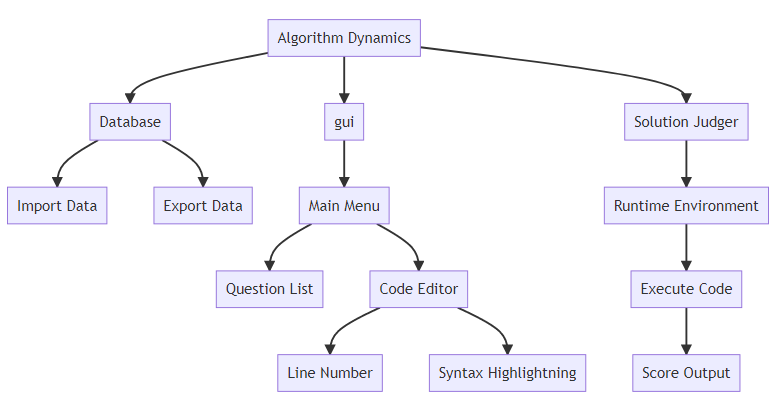
\includegraphics[width=\linewidth]{decomposition-analysis}

\subsection{Thinking concurrently}

When judging the students' solution, many test cases can be executed at the same time to reduce the judging time. The number of parallel judgers needs to be set carefully based on the user's hardware. Running too few test cases concurrently may result in a very long judging time while running too many test cases at the same time may use up computing resources and cause issues.

\section{Interview}

\subsection{Design interview}

\subsubsection{Interview for teachers}

\begin{enumerate}
    \item Do you find your students tend to lose marks on programming questions in exams?
    \item Do you find marking the programming question takes a lot of time and effort?
    \item Compare to the knowledge-based Computer System section, do you find it is more difficult to monitor students' skill level on the Algorithm and Programming section?
    \item Have you ever heard about some online programming platforms?
    \item Have you ever tried some of the online programming platforms?
    \item If yes, what do you think about these platforms? Have you ever considered using them for teaching and training?
    \item Do you think a similar solution can help improve the efficiency of learning and training?
    \item If no, do you think the idea of a software that can mark students' answers on programming questions and provide analysis data can help improve the efficiency of learning and training?
    \item Do you have anything else to add?
\end{enumerate}

Question 1 to 3 is a series of proof-of-concept questions, which I expect my stakeholders to answer `Yes' to all of them. They confirm that the problem I am trying to solve exists and there is a need for such a solution. Question 4 to 5 asks about the teachers' knowledge of existing solutions. Question 6 to 8 ask about their experiences and opinions about these existing solutions, which gives me insights on the problems with existing solutions and how my solution can fit their need better.

\subsubsection{Interview for students}

\begin{enumerate}
    \item Do you find the programming questions difficult?
    \item Do you find yourself lacking efficient practising in algorithm designing and programming?
    \item Have you ever heard about some online programming platforms?
    \item Have you ever tried some of the online programming platforms?
    \item If yes, what do you think about these platforms?
    \item Do you think a similar solution can help you learn and practise?
    \item If no, do you think the idea of software that provides coding questions and marks your answer instantly can help you learn and practice better?
    \item Do you have anything else to add?
\end{enumerate}

Question 1 and 2 are similar proof-of-concept questions to confirm such a problem exists. The following questions ask about students' knowledge of existing solutions. If they have used an existing product before, I ask whether they think it helps. Otherwise, I ask whether they think it will be useful.

\subsection{Conduct the interview}

\subsubsection{Computer Science teacher - Mr Grimwood}

\begin{enumerate}
    \item Do you find your students tend to lose marks on programming questions in exams?

    They do. Many of them don't understand the algorithms.

    \item Do you find marking the programming questions takes a lot of time and effort?

    Yes. Because some students produce partially correct answers, so it takes a lot of time to identify the correct part and award them the corresponding mark. Some students may take completely different approaches which takes a lot of effort to understand and mark them.

    \item Do you find it is more difficult to monitor students' skill level on the Algorithm and Programming section and more difficult to provide sufficient help?

    Yes.

    \item Have you ever heard about some online programming platforms?

    I have. Emm... But I forget the names.

    \item If yes, have you ever tried some of the online programming platforms?

    I have.

    \item If yes, what do you think about these platforms?

    I think the idea is quite interesting and I find them working quite well.

    \item Have you ever considered using them for teaching and practising?

    No. Because most of them require a paid subscription, and their content is more likely to be something like `Learning Python' which is irrelevant to the A Level Computer Science content.

    \item Do you think a similar solution can help improve the efficiency of learning and training?

    Yes. The students can learn at their own pace and they can keep practising by themselves.

    \item Do you have anything else to add?

    No.
\end{enumerate}

Mr Grimwood has several valuable points here. He points out that the `partially correct' answers are the most difficult ones to mark. For my solution, if a student submits a `partially correct' code answer, then its output will certainly not match the expected output. This means my solution might not be able to tell the difference between a `partially correct' answer and an `incorrect' answer. This is a potential limitation I need to watch out for. He also says the price is one of his concerns. My solution will be free and open-source, which will meet his need perfectly. By adding the function to create custom questions and share them with others, users will be able to create and find A Level Computer Science content, or any content easier. It is also a good idea for me to create some A Level Computer Science content that comes with the software to make it easier to use.

\subsubsection{Computer Science student - PCloud}

\begin{enumerate}
    \item Do you find the programming questions difficult?

    I find some of them quite complex and difficult, especially the graph algorithms such as Dijkstra.

    \item Do you find yourself lacking efficient practising in algorithm designing and programming?

    Absolutely. Although I code a lot in my spare time, normal projects are quite different from the exam questions. There are not many past papers and exam-style questions for practising, so I usually don't feel confident of those questions.

    \item Have you ever heard about some online programming platforms?

    Yes. Such as AcWing, LeetCode, and TopCoder.

    \item Have you ever tried some of the online programming platforms?

    Yes. I am an active user of AcWing.

    \item If yes, what do you think about these platforms?

    I enjoy the experience. They can provide instant feedback for my submissions. It provides very strong positive feedback when I solve a new question. I find myself learning faster and more efficiently with such platforms.

    \item Do you think a similar solution can help you learn and practise?

    Absolutely. The existing platforms do not provide A Level related content. So if a software solution can be altered for A Level Computer Science course, that will help a lot.

    \item (*) How do you think it should be optimized for A Level CS content?

    You can add past exam questions practising. Adding a timed practice mode will be helpful.

    \item Do you have anything else to add?

    No.
\end{enumerate}

PCloud confirms that such a solution will help him learn and practise more efficiently. The instant feedback of whether he gets the question correctly is very important to him. Instead of sending the user's submission to a remote server, my solution should judge the user's answer on their computer. This can avoid the instabilities caused by the remote server's availability and the network connection. He also gives me some good ideas about the content. I can add past exam questions for users to do timed practice, which enables users to practice algorithms and exam techniques at the same time.

\subsubsection{Computer Science student - Timofei}

\begin{enumerate}

    \item Do you find the programming questions difficult?

    Yes. I generally lose marks because of some careless syntax mistakes I made.

    \item Do you find yourself lacking efficient practising in algorithm designing and programming?

    Yes. I find I cannot find many materials to practice.

    \item Have you ever heard about some online programming platforms?

    Codewar. Something like that.

    \item Have you ever tried some of the online programming platforms?

    Yes.

    \item If yes, what do you think about these platforms?

    I think they are quite helpful. But I find their marking is too specific, if I get a single character wrong in my output, it gets marked incorrect.

    \item Do you think a similar solution can help you learn and practise?

    Yes.

    \item Do you have anything else to add?

    No.

\end{enumerate}

Timofei points out that the marking system in existing products is not very sensible. This may be a potential limitation of my solution as well. It is easy to directly compare the users' output and the expected output. But if they are different, it is difficult to figure out whether that difference is caused by a wrong code solution or just some formatting error. I can partially solve this by allowing the users to pre-test their code against examples before formal submissions, so they can check the output format.

\section{Research}

There are many coding training websites on the market, most of them share a similar idea, so I will investigate two of the most popular ones.

\begin{itemize}
    \item LeetCode
    \item Codeforces
\end{itemize}

\subsection{LeetCode}

\href{https://leetcode.com/}{LeetCode} is a platform for interview coding training, many large companies (Google, Facebook, ...) use it as a part of their interview.

LeetCode provides a database containing more than 1000 coding questions.

\subsubsection{Main coding layout}
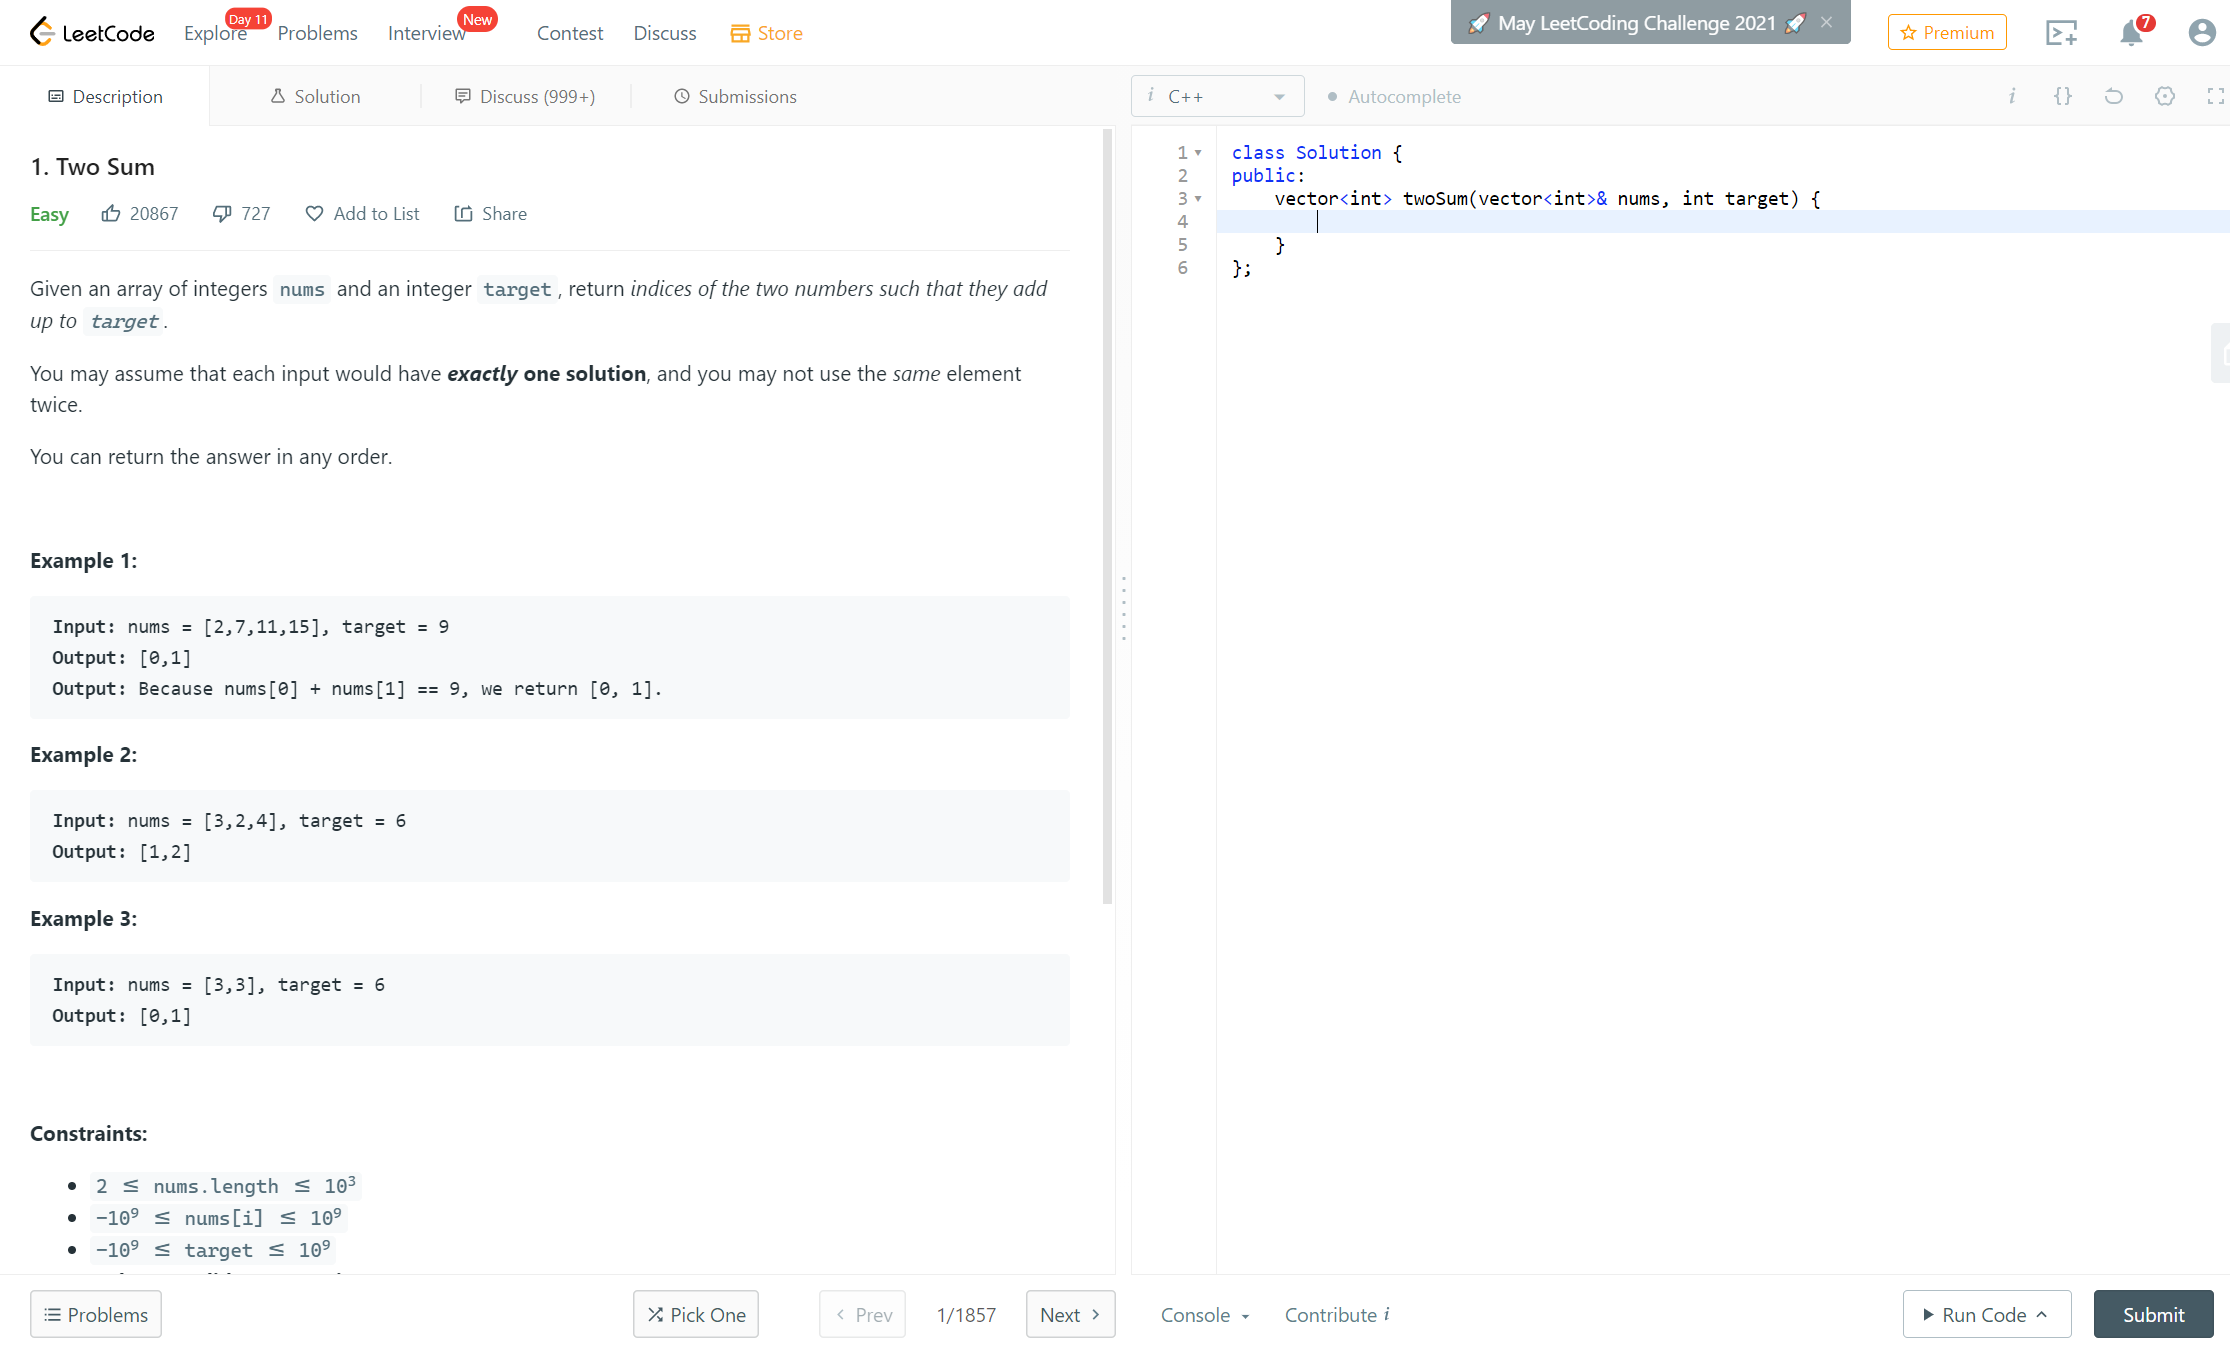
\includegraphics[width=\linewidth]{Two-Sum-LeetCode-Coding}

This is LeetCode's main coding area. The user's screen is split into two parts - the question section and the code editor for inputting answers. Users can drag the splitter in the middle to adjust the size of each section.

The question section contains 4 tabs, `Description' tab displays the content of the question. `Solution' tab displays the solutions from the community. `Discuss' tab displays the discussions in the community. `Submission' tab lists the user's previous submissions. Since I am not adding social functions in my solution, I will ignore the `Solution' and `Discuss' tabs. Under the `Description' tab, LeetCode provides the context of the question, followed by 3 examples, and constraints for this question. The examples allow the user to run and check their solution before formal submission for marking, this can help them avoid silly mistakes. My solution should also provide similar examples for each question. Under the `Submission' tab, LeetCode records every history submission, so the user can revise old questions more efficiently. My solution should provide a similar function as well.

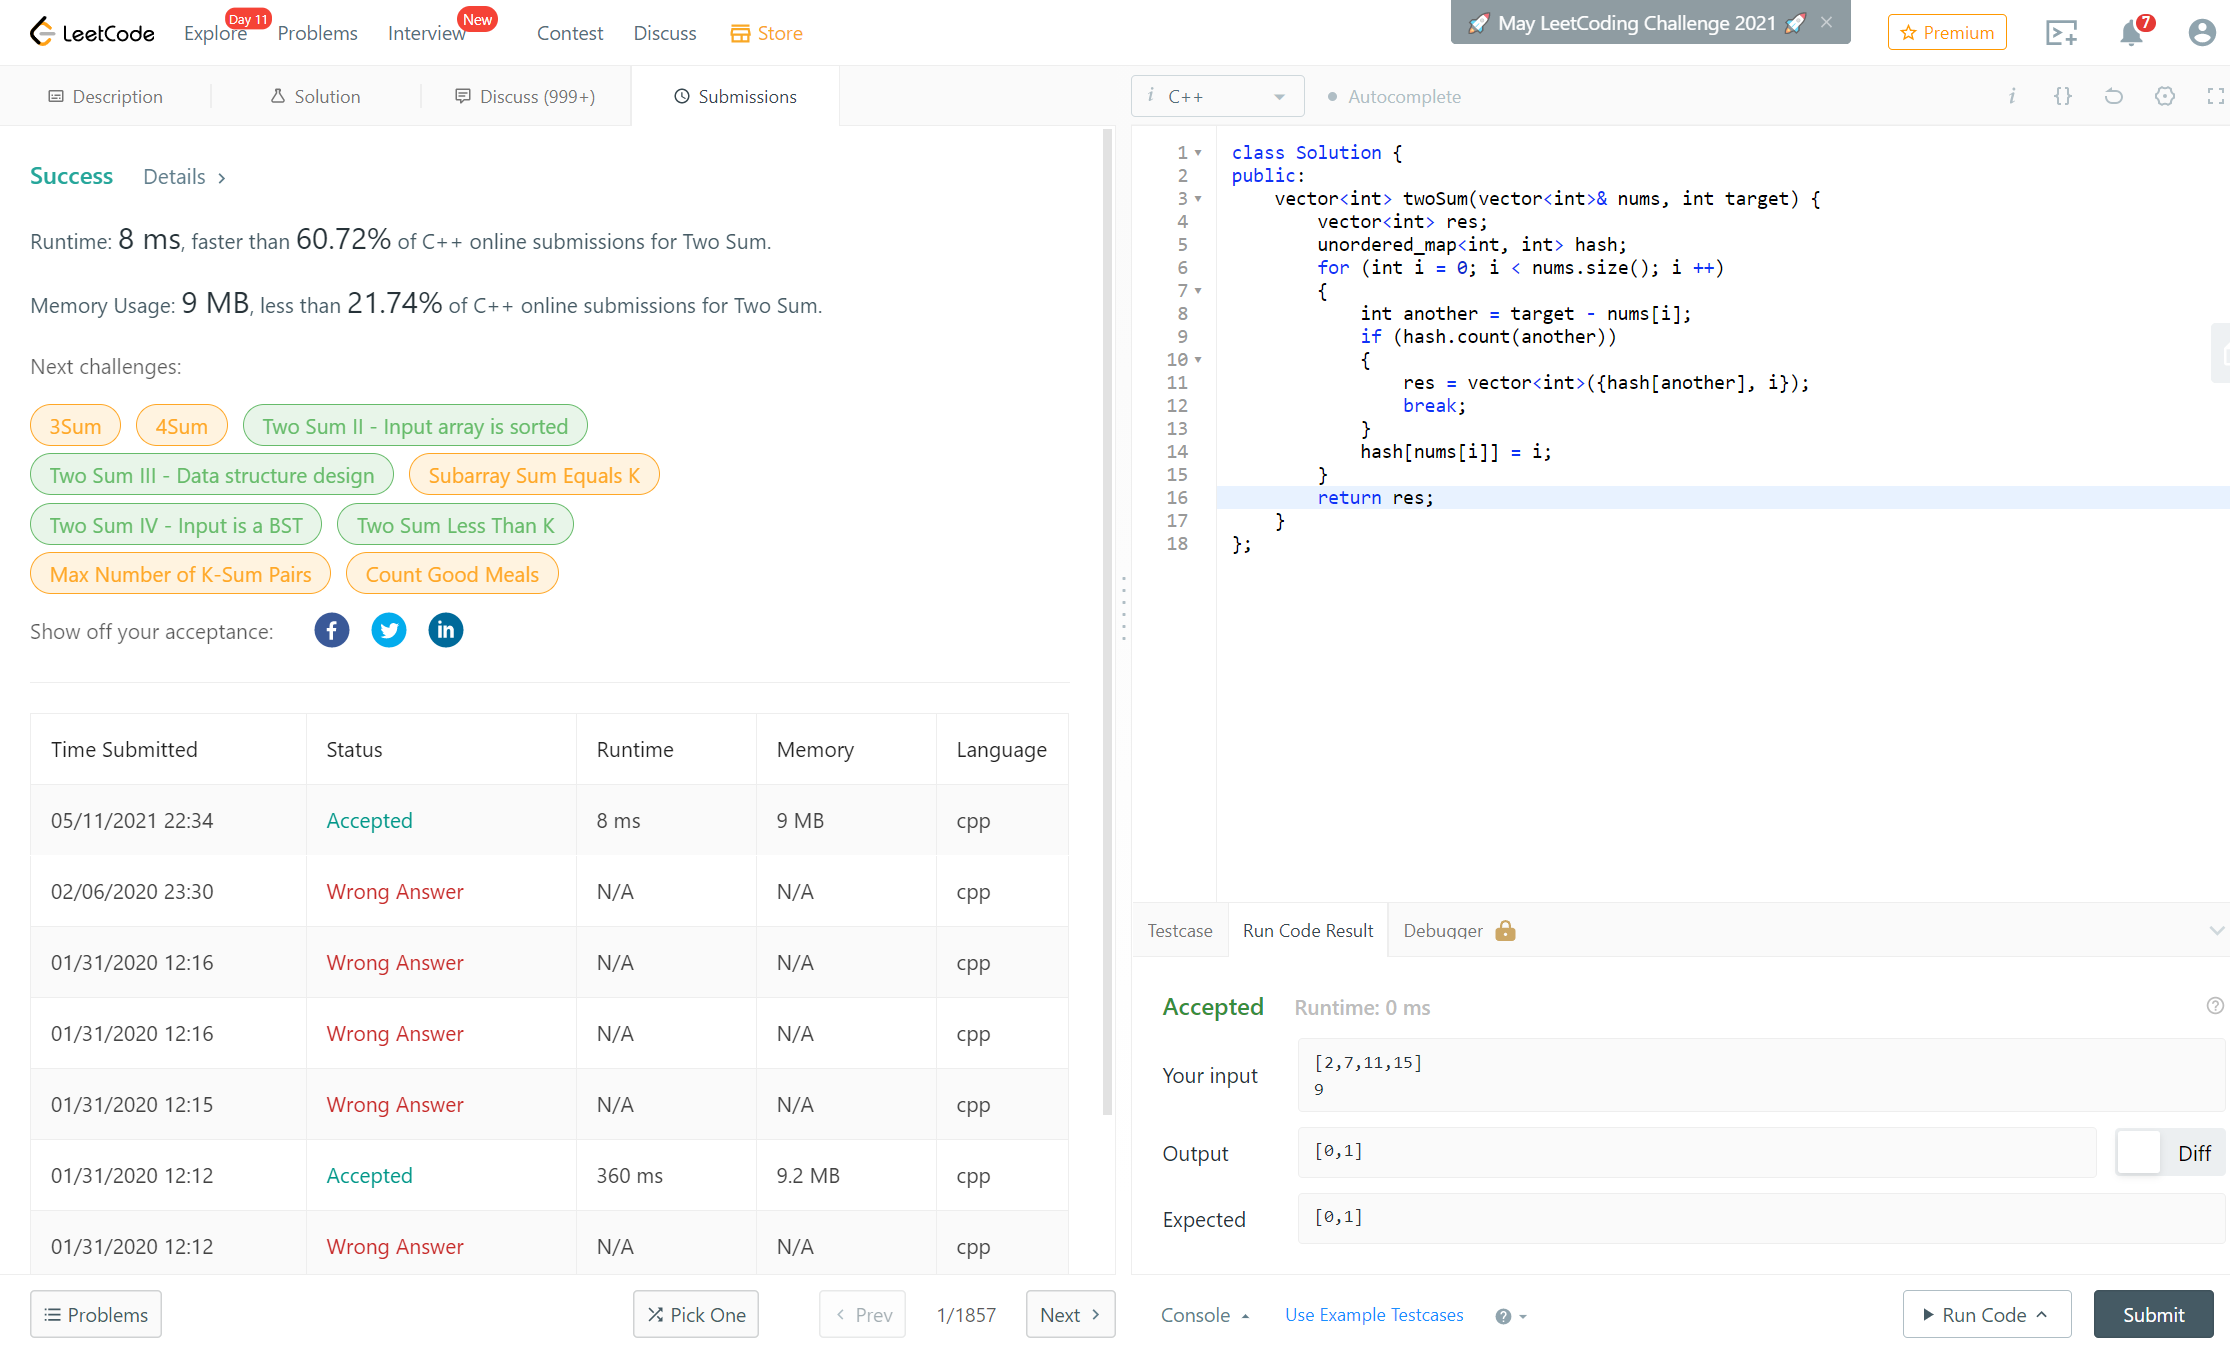
\includegraphics[width=\linewidth]{Two-Sum-LeetCode-Submission}

The code editor provides line number and syntax highlighting functions. User can change their programming language with a drop-down box. LeetCode supports all mainstream programming languages. My solution should be able to support multiple programming languages as well, which allows students with different backgrounds to use them easily.

On the button, the user can `Run Code' to test their code against the examples before submission, and then click the `Submit' button to submit their solution formally.

The split view design is clean and handy. The user can see the question and write their solution on the same page without switching between different windows. The design of examples and the `Run Code' button is useful as well. I can refer to LeetCode's coding layout when designing my solution's interface.

\subsubsection{Question database}

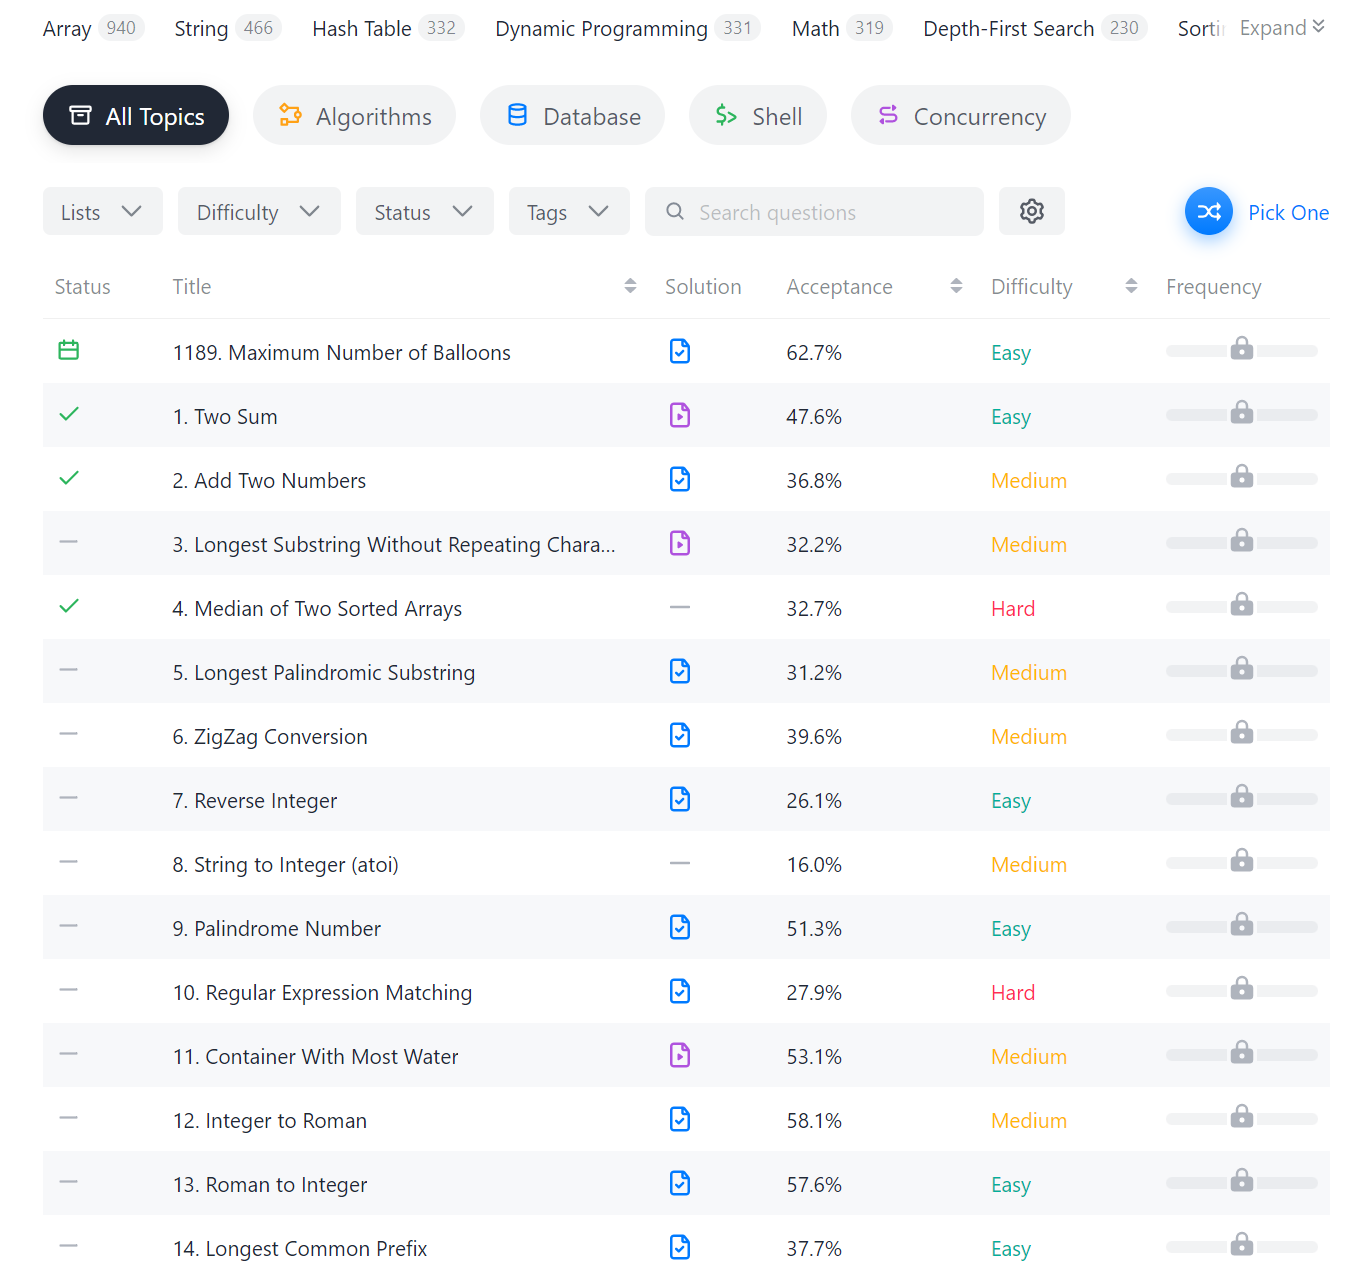
\includegraphics[width=\linewidth]{LeetCode-Problems}

Every question in LeetCode has many different attributes (Lists, Difficulty, Status, Tags, Title, Acceptance), so it is very easy for a user to find a suitable question to practice. My solution can similarly organize the question database and provide a corresponding query interface for a better user experience. The Pick One button on the top right is a very handy feature as well. Users can simply click that button to start working on a quick random question. The idea of a list of questions is great. Users can organize a series of questions to practice and share.

\subsubsection{Pricing}

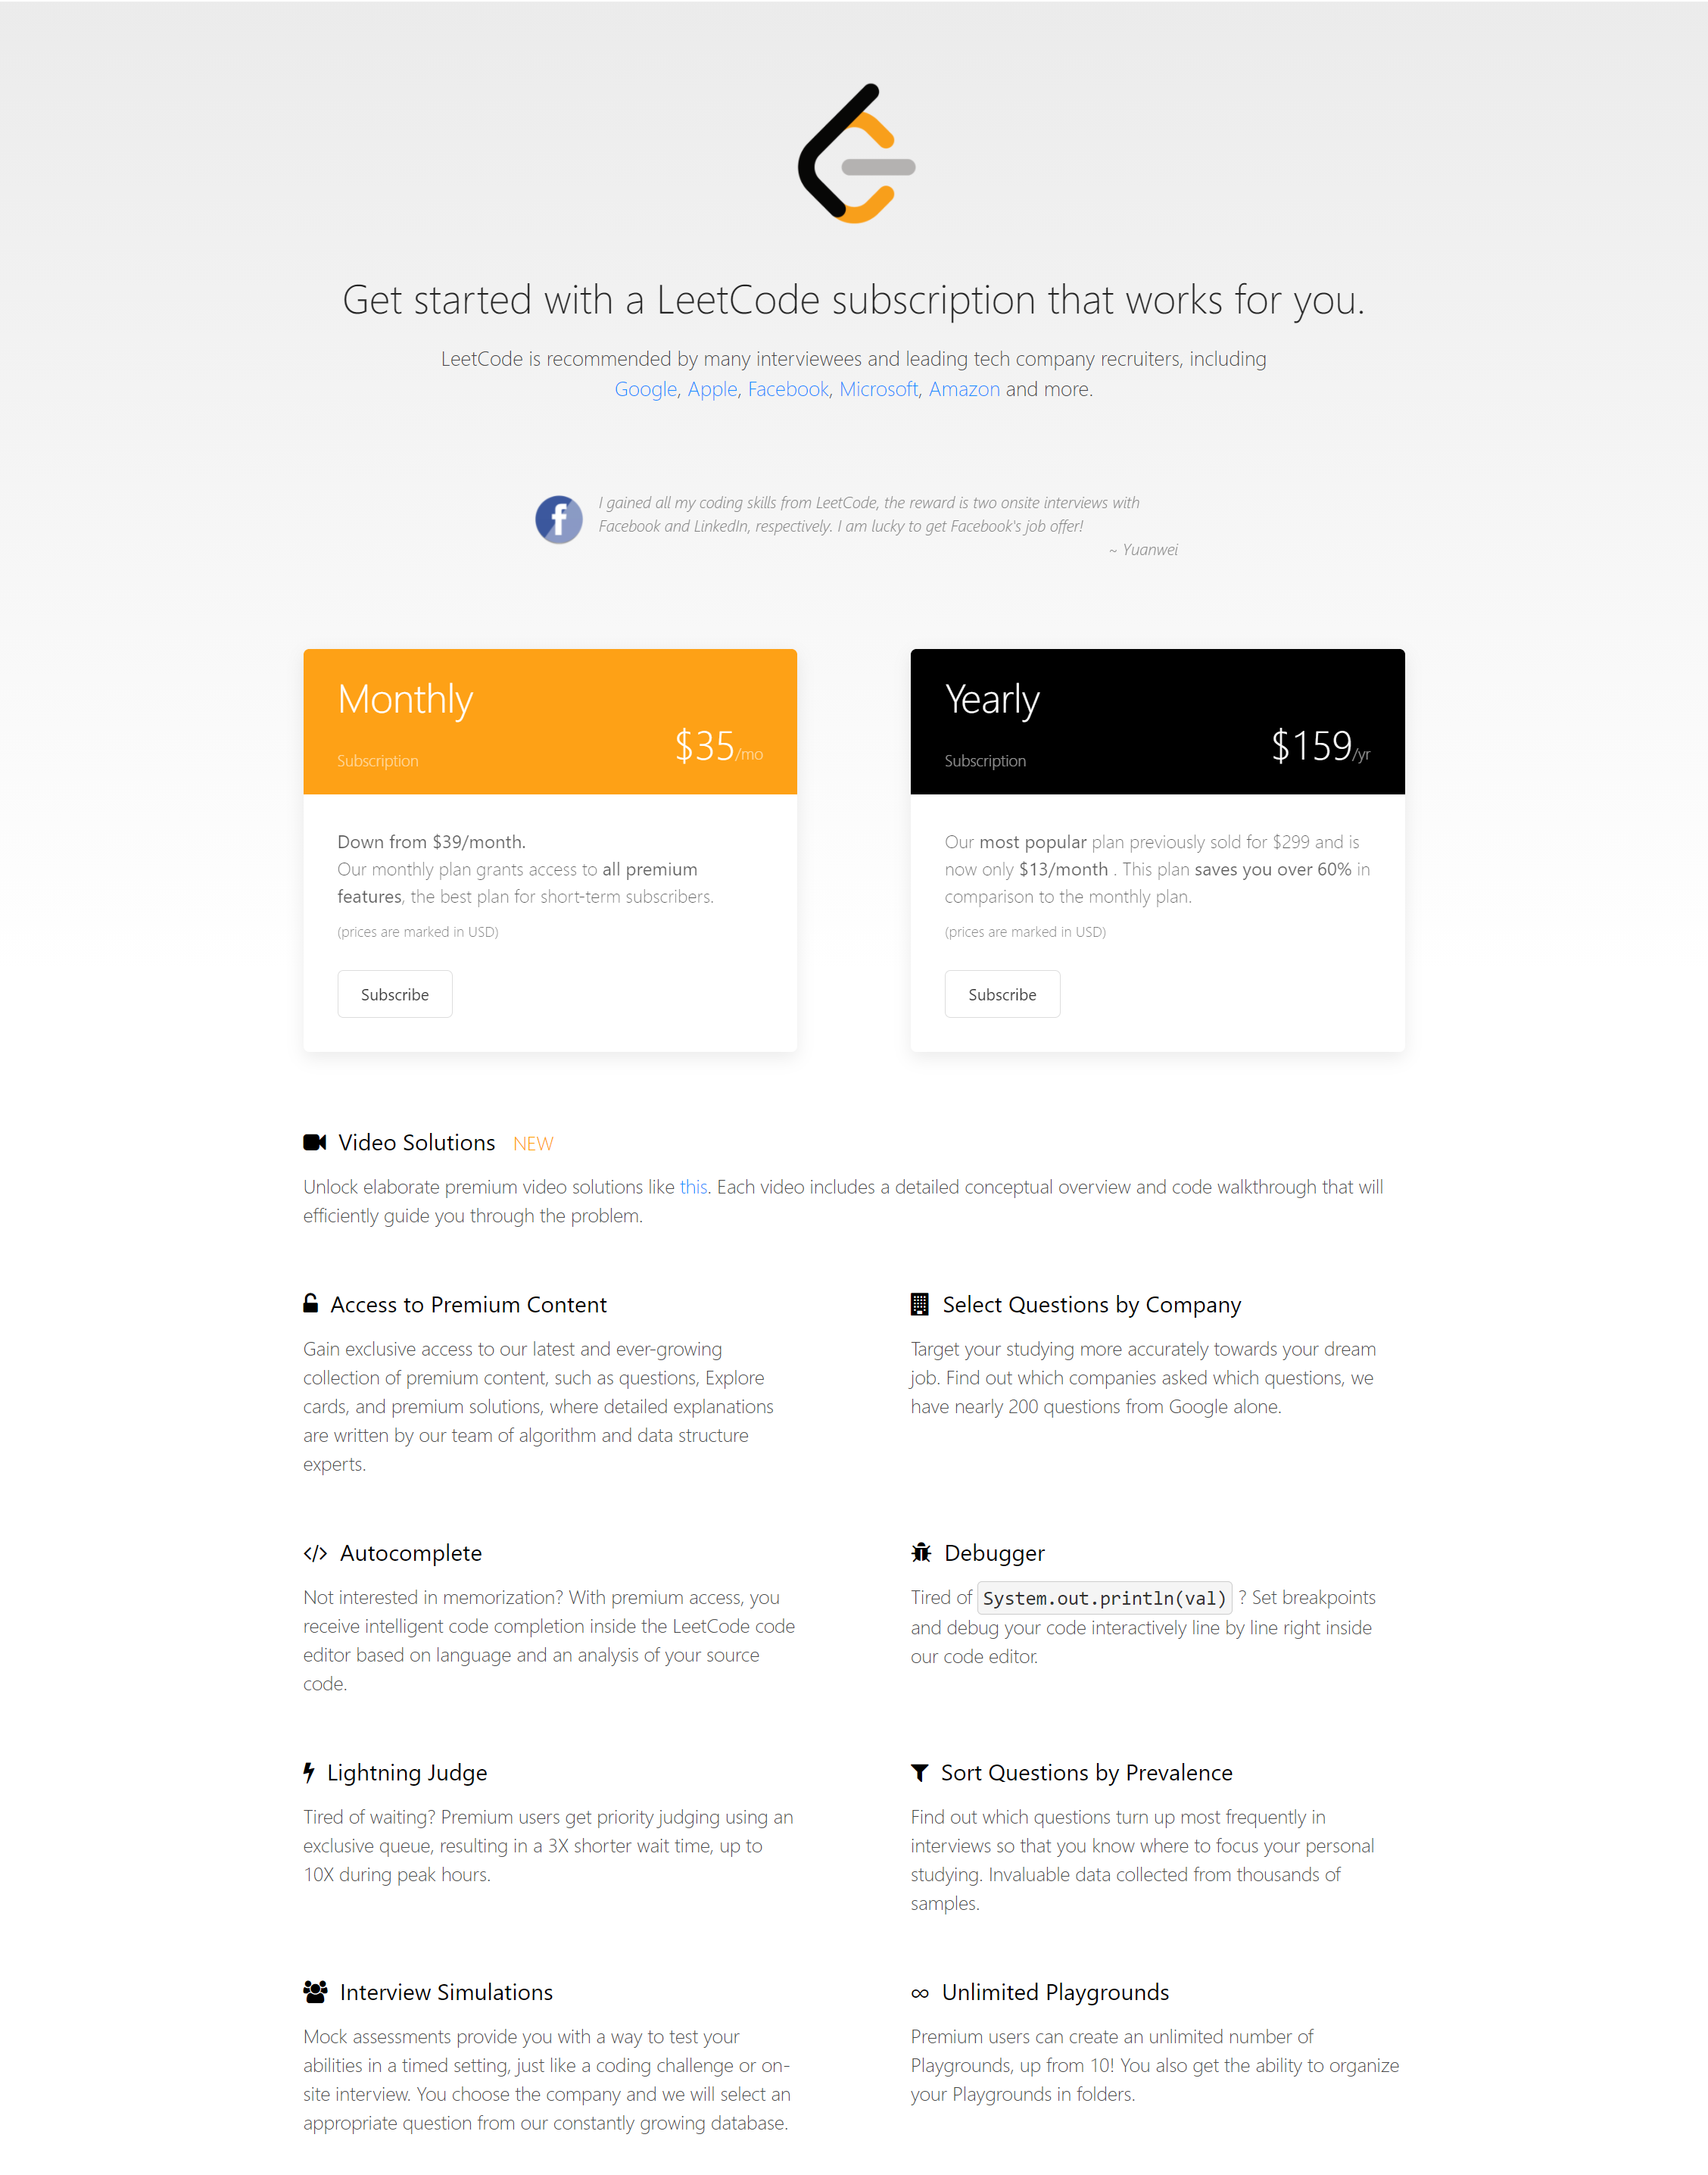
\includegraphics[width=\linewidth]{LeetCode-Premium}

The basic functions of LeetCode are free to use for all users and it charges a fee for premium subscriptions. The premium subscription provides a larger question database, better code editor, faster judger, and more.

\subsubsection{Analysis}

LeetCode is a fully web-based solution, which means it works on any device. However, it also means you will not be able to use it without a stable Internet connection. I decide to make my solution a desktop application since most students practice coding with a computer. It also save me a lot of cost from running and maintaining a server. LeetCode runs a large community for users to discuss questions with each other. I am not adding such a function to my solution. Teachers and students can use existing platforms they have been familiar with, it is unnecessary for me to develop a new platform and for the users to migrate from mature solutions. LeetCode has an easy-to-use graphical interface, which is important so new users can get their hands on very easily.

LeetCode does not support custom questions or any functions for educators. It is mainly designed for self-learners. My solution is designed for school use, so it must support functions like custom questions, custom assignments, statistics data visualizations. LeetCode charges a subscription fee for essential functions. My solution will be free and open-source so everyone can benefit from it.

\subsection{Codeforces}

Codeforces is a competitive coding platform, it is mainly used by people to hold coding competitions.

\subsubsection{Main question layout}

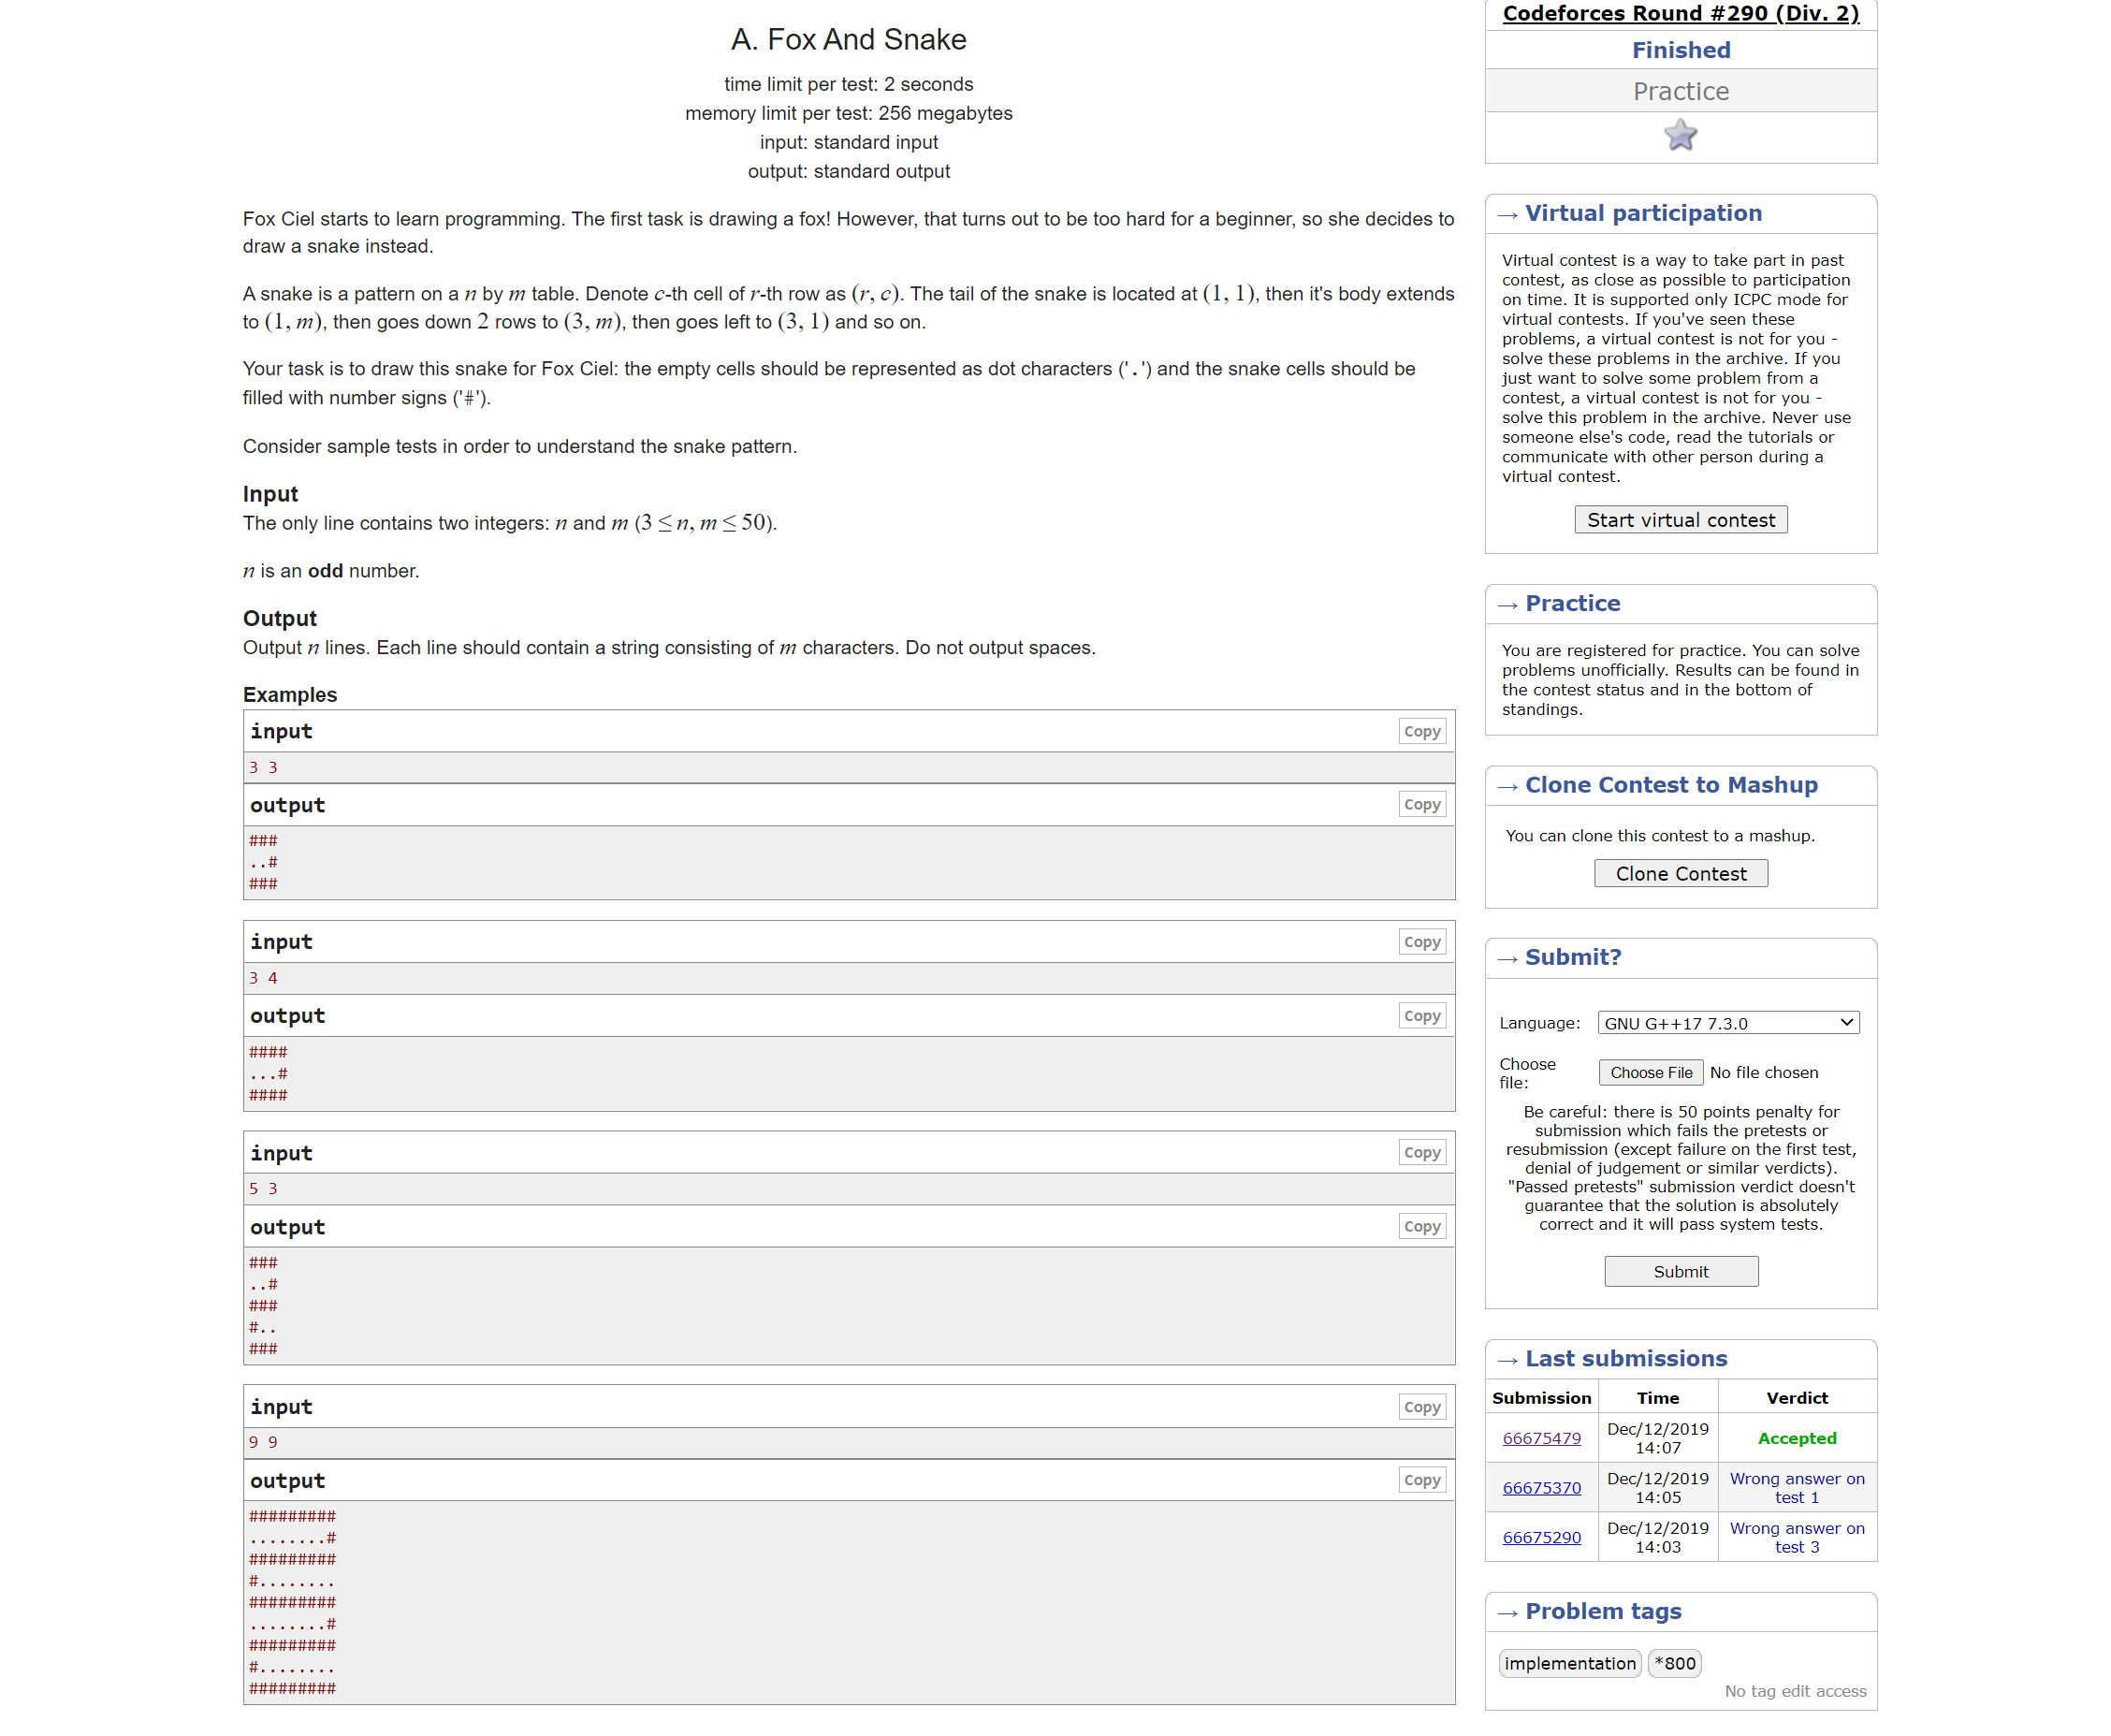
\includegraphics[width=\linewidth]{Problem-A-Codeforces}

The questions and the examples take up nearly all the spaces on the question page. There is no online editor or online runtime environment provided. Users are expected to write and test their code in their IDEs and only submit the solution for judging. Custom IDEs may be more powerful than a built-in one. My solution will provide an editor, it is much more convenient to use. Even if a user decides to use his environment, he can paste his code into the editor for submission. It sets the time and memory limits for users' submissions, if a piece of code takes too long to run, or takes up too much memory while running, it will be terminated and marked wrong.

\subsubsection{Submission}

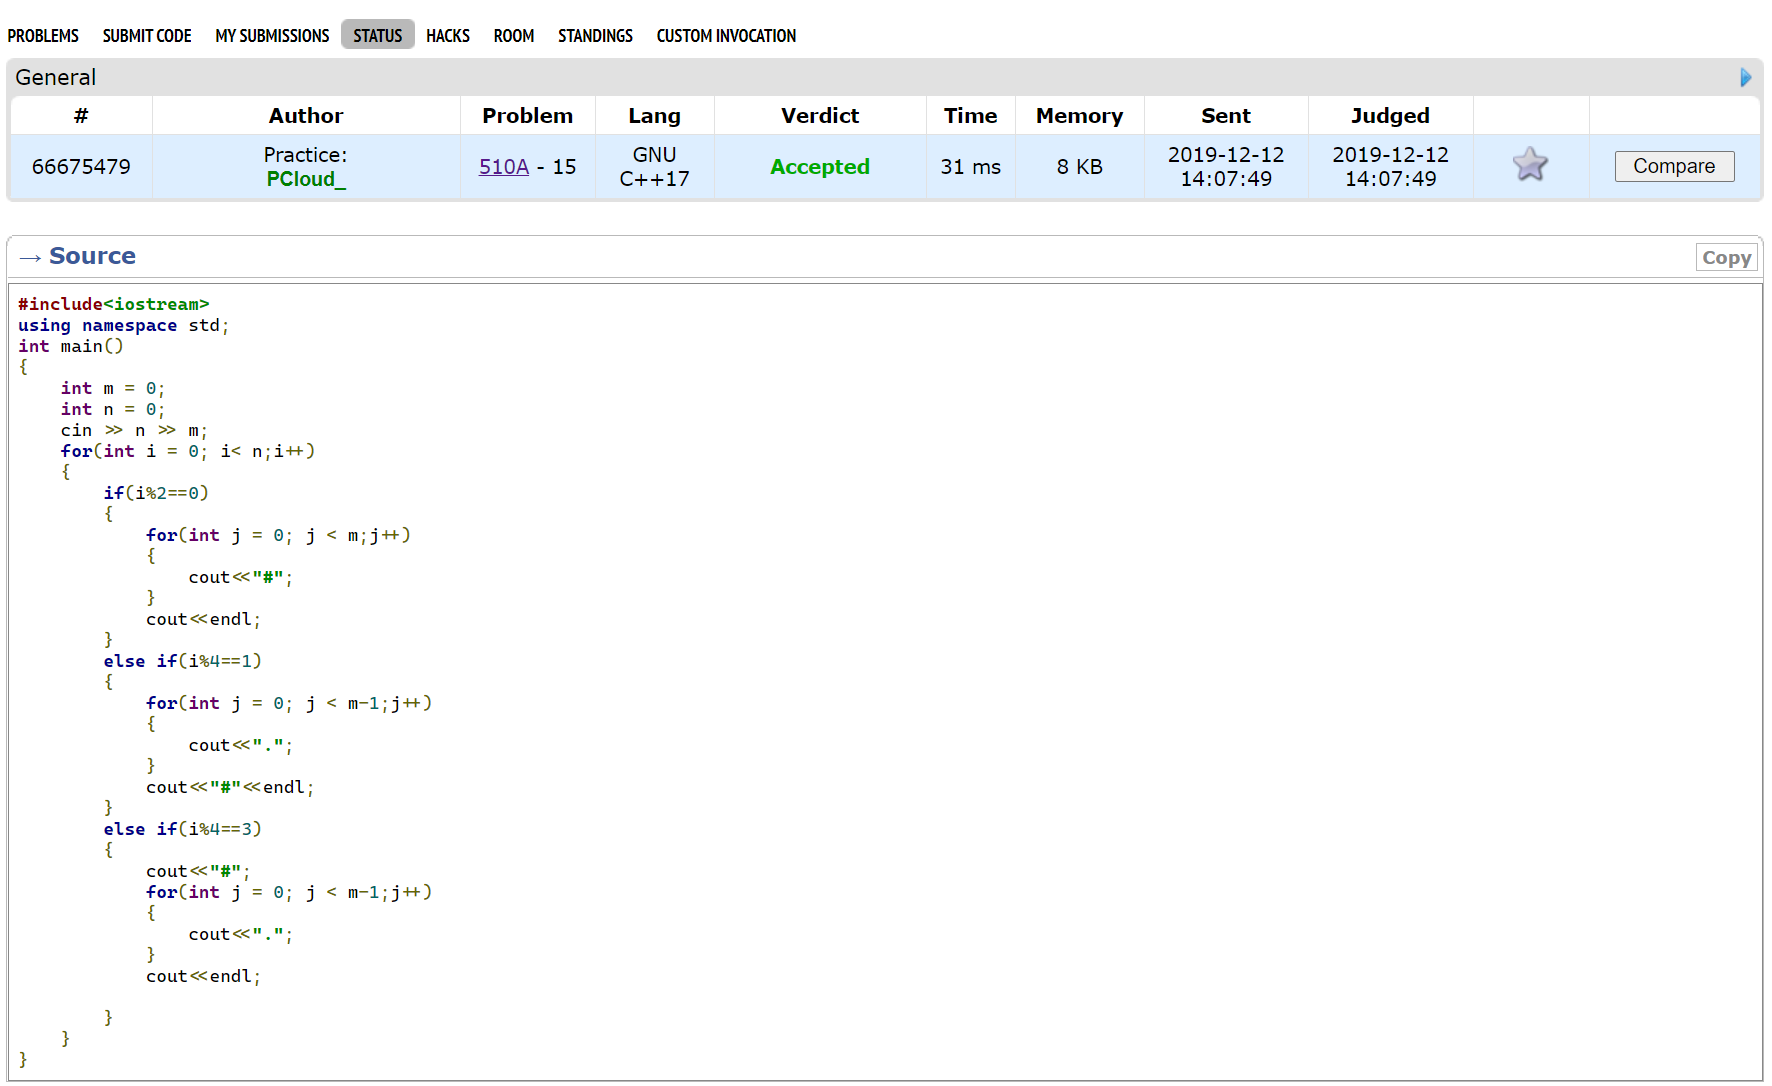
\includegraphics[width=\linewidth]{Submission-66675479-Codeforces}

When the user submits the code, the code enters a queue waiting for judging, then the user can look up their result. Users can check their source code, performance stats, and more importantly, when they have not passed all test cases, they can see what they have got wrong. The judgment protocol provides detailed information about each test case, so users can debug easily.

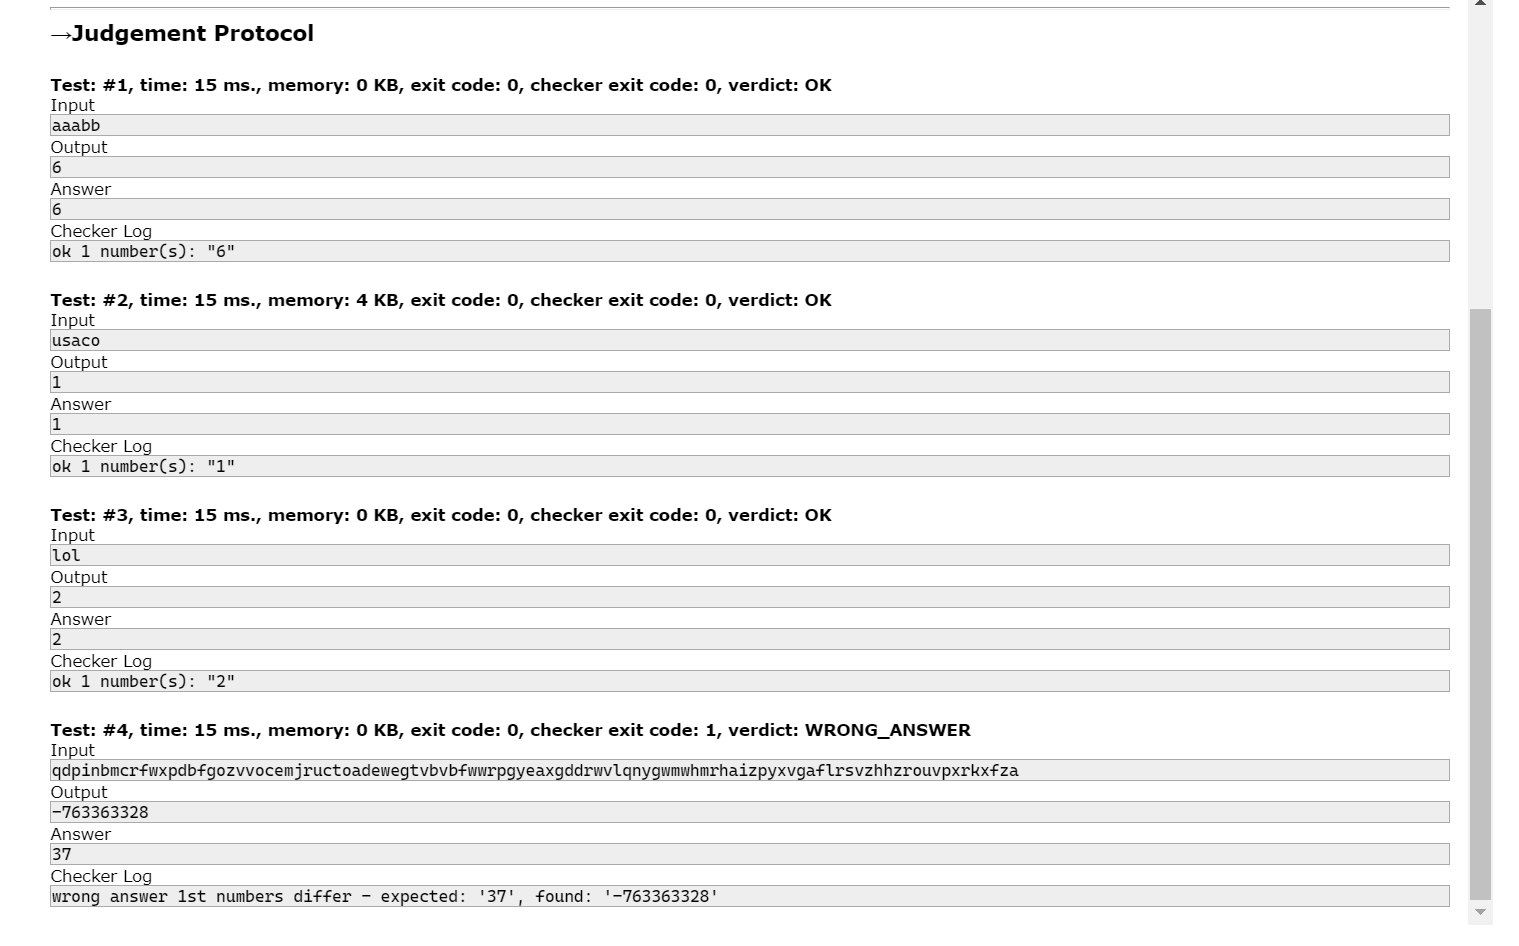
\includegraphics[width=\linewidth]{Judgement-Protocol-Codeforces}

\subsubsection{Analysis}

Codeforces is optimized for coding competition, so it has a lightweight and complex interface for better performance. It is completely free to use. Users can create their questions but it is very complicated to do so. My solution needs to enable users without experience to create questions easily. There is no function for education - there is no way for a teacher to `create a class' and monitor his students. Codeforces is an online platform, so it also works across all devices and requires an Internet connection. Users have to use their IDEs to write and debug their code. Codeforces sends all submissions to a central `judging queue' for marking. My solution will mark all submissions locally, which makes judging a lot faster and save me from running a server. By limiting time and space allowance, Codeforces effectively prevents malicious code from running.

\section{Features}

A useful homepage interface with shortcuts to different functions in the software and other resources outside the software. This allows the user to get into practising faster and makes the software easy to use. Details about the design of the homepage will be discussed in the Design chapter.

A problem database with a graphical user interface. The GUI will have a search box and several drop-down menus for the user to input information to search for a problem. This provides the user with a simple way to find the problems they want, and it also ensures the users can manage and backup the data easily.

An interface for users to create new problems and share them with others. This interface will have multiple text fields for the user to input the descriptions to the problem, the expected input/output data. Then the problem is saved to the database and can be exported to a JSON file allowing the user to share it with others. Users can also create a `list' of problems and export the entire list into a JSON file and share it with others. This enables teachers to create custom problems and share them with the students. It is a core feature that differentiates my solution from the existing ones.

An interface for teachers to create assignments. An assignment is a `list' of problems with some extra data, such as the due date and total mark. It can be exported to a JSON file and shared with students. The student's submission will be exported into a JSON file as well and can be sent back to the teacher. The solution will also integrate with the assignment function in Microsoft Teams for Education, which makes it even easier to do. The students' submissions will be automatically marked by the software and detailed data will be provided to the teacher. A simple data analysis interface will be provided to the teacher so they can have a brief look at the result. The teacher can also export the data into a CSV file so they can import it to their school system or analysis it with professional software. This automates the entire process from creating assignments, distributing assignments, collecting assignments, and marking assignments. Teachers will have more time analysis the student's performance and provide corresponding help timely. It is a core feature that differentiates my solution from the existing ones.

An interface displaying the problem and the code editor. The solution provides a `Run Code' button for the student to pre-run their code before submission, a `Submit' button for the student to submit their code. This allows the students to read the question and write their code solution without switching between different windows. The `Run Code' function also makes it easier to debug their code.

A playground with a code editor and runtime environment. This allows the software to be used in class teaching as well, the students can experiment with different algorithms and programming languages in the playground easily.

A settings page contains all the setting options for the software. Users can adjust settings such as their preferred programming language, syntax highlighting settings, colour themes, and so on. This allows the users to customize the software to fit their needs and allows users with different backgrounds to use it without issues.

\section{Limitations}

The software will be written in C\# instead of web-based which means extra software needs to be downloaded by the user. I plan to use .NET 5 runtime and WinUI 3 library for my solution, so only the Windows 10 1809 or newer Windows operating systems will be supported. This should not cause many compatibility issues since most school computers are running the required version of the operating system. Downloading extra software is inconvenient and may violate the IT security policy of some schools.

The judger can only accept limited programming languages and the user may require to configure their runtime environment. Creating a compiler for `OCR Pseudocode Programming Language' is too complex for this project. I will attempt to allow the user to add their preferred programming language and write documentation for them to make the process easier.

Unlike LeetCode, there are no Discussion pages for users to discuss questions because it is a desktop program instead of a web one. But this is not a big problem, students and teachers should use an existing product such as Microsoft Teams which has very good support in sharing code snippets. It is unnecessary to rebuild the wheel.

Distributing the questions and assignments is still inconvenient. Currently, distributing questions and assignments requires the teacher to first export the questions and assignments, then send them to the students through email or file-sharing platforms. When the students finish working, they need to send their results back through email or other apps. I have attempted to integrate the file-sharing function with the existing platform - the Microsoft Teams Assignment function. But unfortunately, the Graph API required for this operation is still in beta version, which means it can only be tested in the development environment and cannot be used in production. So for now, the users still have to use this inconvenient way to share questions and submissions. But in the future, the integration with some existing platforms may improve the experience. (Update: the Microsoft Teams API is out of beta, now it is possible to integrate with it)

There are no good ways to maintain and distribute a large question database. Computer Science teachers are required to maintain a database for their students. But this is difficult work. Creating good test cases is much time consuming than writing a mark scheme, it is very likely for a wrong solution to pass the judging if the test cases are not good enough. It relies on the teacher who creates the questions to consider everything clearly to minimize its impact.

The judger can only simply compare the students' output with the expected output if there is a format error such as trailing space and extra newline in their output, which will not be considered as a mistake in a real exam, will be marked as a wrong answer by the judger. So students may need to spend extra time debugging their output format. It cannot judge ``partially correct'' answers as well. It does not care which line did the student get correct or wrong, if the final output doesn't match, the submission will be marked wrong.

\section{Hardware and software requirements}

\begin{tabulary}{\linewidth}{|L|L|}
    \hline
    Hardware and software requirements & Justification \\
    \hline
    Standard mouse, keyboard, and monitor. & Standard I/O devices are required for the user to interact with the software. Users need a mouse to navigate around different menus and pages, they need to use a keyboard to input their code solutions and use a monitor to get the output from the software. \\
    \hline
    Operating system: Windows 10 (1809 or later), Windows 11. & The software is designed with the WinUI 3 library and .Net 5 runtimes, which require such an operating system to run. \\
    \hline
    x86 64-bit CPU (Intel / AMD architecture) with 2 or more cores and 1 GHz or higher clock speed. & A modern CPU is required for the software. 1 core will be used to run the main program and at least 1 spare core is required for the judger to judge the submitted code. A clock speed higher than 1 GHz is required to ensure the software is running smoothly. \\
    \hline
    1GB free memory or more. & Around 512MB RAM is required to run the software, and another 512MB RAM is required for the judger to judge the submissions. \\
    \hline
    256MB free disk space or more. & 256MB free disk space is required to store and run the program itself, the user may need extra disk space to store extra cache data and the database. \\
    \hline
    A modern dedicated or integrated graphics card. & The software has very little graphical demand, if the user's graphics card can run their operation system, it should be able to handle software as well. \\
    \hline
\end{tabulary}

\section{Success criteria}

\subsection{User experience criterias}

\subsubsection{Easy navigation around the software}

The user can use different links, menus and buttons to navigate around the software easily. This makes the app easy to use and allows the user to find the function they want quickly. This is also essential for the students and teachers to get their hands on the app right away without the need of reading a long documentation about the software.

\subsubsection{Easy to find data in the database}

The user can use an advanced search tool to search any problems or problem lists from the database easily. This allows the user to quickly find the problem they want from the database and improves their productivity.

\subsubsection{Easy to create new problems}

The users should be able to use a simple but powerful interface to create new problems in the database. The user should only be asked to input necessary data about the new problem, and these data should get validated automatically. The user should be able to see a preview of the data while creating the problem, which allows them to make sure the data is correct before submitting it to the database.

\subsubsection{Easy to create problem lists}

The users should be able to search for problems and add them to a list easily. They should also be able to name the list and add a description to it. This allows the user to group the problems easily and share with others.

\subsubsection{Assignments functionality}

The teachers should be able to create assignments from problems and distribute them to the students. The students should be able to complete the assignments and submit their solutions back to the teacher. The teacher should be able to auto grade the submissions and give feedback to the students. This fully automates the process of algorithm teaching and learning and grading, which is one of the problems the app tries to solve.

\subsubsection{Microsoft Teams integration}

The user should be able to login their Microsoft account, and interact with the assignments through Microsoft Teams. This utlize the existing architecture of digital teaching in the stakeholders' school, which makes the entire process more efficient and less time consuming.

\subsubsection{Playground functionality}

Provide the user with a playground to run code in different programming language quick. This is particularly useful in in-class teaching. The students can practice on writing code for an algorithm immediately after teaching.

\subsubsection{Custom settings options}

Provide the user with a set of customizable settings options. This allows the user to customize the settings of the software to their liking. The settings should be stored on the disk automatically, and should be deleted when the app is uninstalled.

\subsubsection{Account settings}

Provide the user with a set of account settings. This allows the user to change their account information, such as username, password, and email. The account information is attached to submissions and assignments for the interaction between teachers and students.

\subsection{Technical criterias}

\subsubsection{Local Database}

Create and maintain a local database to store all the user data inside. Use custom commands to query the database and return the results to the frontend without any additional setup from the user. The database should also be cleared when the user deletes the software.

\subsubsection{Prevent SQL injection}

Measurements should be taken to prevent SQL injection. This is a common problem in database applications. The software should prevent SQL injection by using prepared statements and parameterized solution. Therefore the database will not be destroyed by improper input.

\subsubsection{Data validation}

All input boxes should be validated when the user is inputing and any data that is invalid should be rejected right away. A clear and concise message should be displayed to the user to explain what has gone wrong.

\subsubsection{Code Editor}

A robust and well-designed code editor needs to be implemented to provide the user the best possible experience writing code inside the app. The code editor should support syntax highlighting for all common programming languages, line numbers and basic editing functions.

\subsubsection{API calls}

The app should handle the APIs of the Microsoft Graph API. It should be able to handle the OAuth2 login, access education data through various endpoints and handle different responses and exceptions gracefully. This provides a robust foundation for the Microsoft Teams intergation.

\subsubsection{Meaningful variale name}

All variables should have sensible names. This helps me understanding my own code in the future developement and make the codebase easy to maintain. The naming convention should follow the Naming Guidline\cite{microsoft:docs:naming-guidelines} from the dotnet framework documentation. 

\subsubsection{Comments}

Comments should be added for every function and any important code. This helps me understanding my own code in the future developement and make the codebase easy to maintain.

\subsubsection{Object Oriented Design}

The object oriented programming should be used across the entire codebase. Every page, window, data model should be abstracted into classes. The app should build on top of the interaction of different instances of data models. This makes the app easy to maintain and enable me to reuse different components and improve developement efficiency.

\subsubsection{Modular design}

The app should be split into different small projects. A main project contains the user interfacen and the integration with other projects. A core project is used to implement all core functionalities. A test project is used to conduct unit testing on the main and core project. Splitting into smaller projects organizes the codebase and make it to be more manageable and easy to maintain.

\subsubsection{Unit testing}

Unit testing is a testing tool that lets me write test cases in code to test different components of my code. These tests can be run automatically after changes to the codebase. This improves the efficiency of the testing significantly comparing to test everything by hand. Which helps eliminating the bugs during developement stage and prevent future features from affecting existing features.

\subsubsection{Continuous integration and continuous delivery}

Continuous integration means after every change to the codebase, the code is send to a remote server. The app is then built and tested on the server, only if the app passes all the tests and build successfully, the change of code can be merged into the codebase. This helps me improving the code quality throughout the developement and eliminating bugs efficiently. Continuous delivery means every time when I create a new release, the app is automatically build and published to the Microsoft Store for the stakeholders to download. This makes delivery faster with better code quality. It also allows the stakeholders to give me feedback instantly after I make any changes, which allows me to work with them better.

\chapter{Design}
\section{Decomposition}

As shown in the decomposition diagram on the next page, the entire problem will be decomposed into 5 main sub-problems: user interface, judger module, database module, data structure design and API module. Each of which will be further decomposed as explained below.

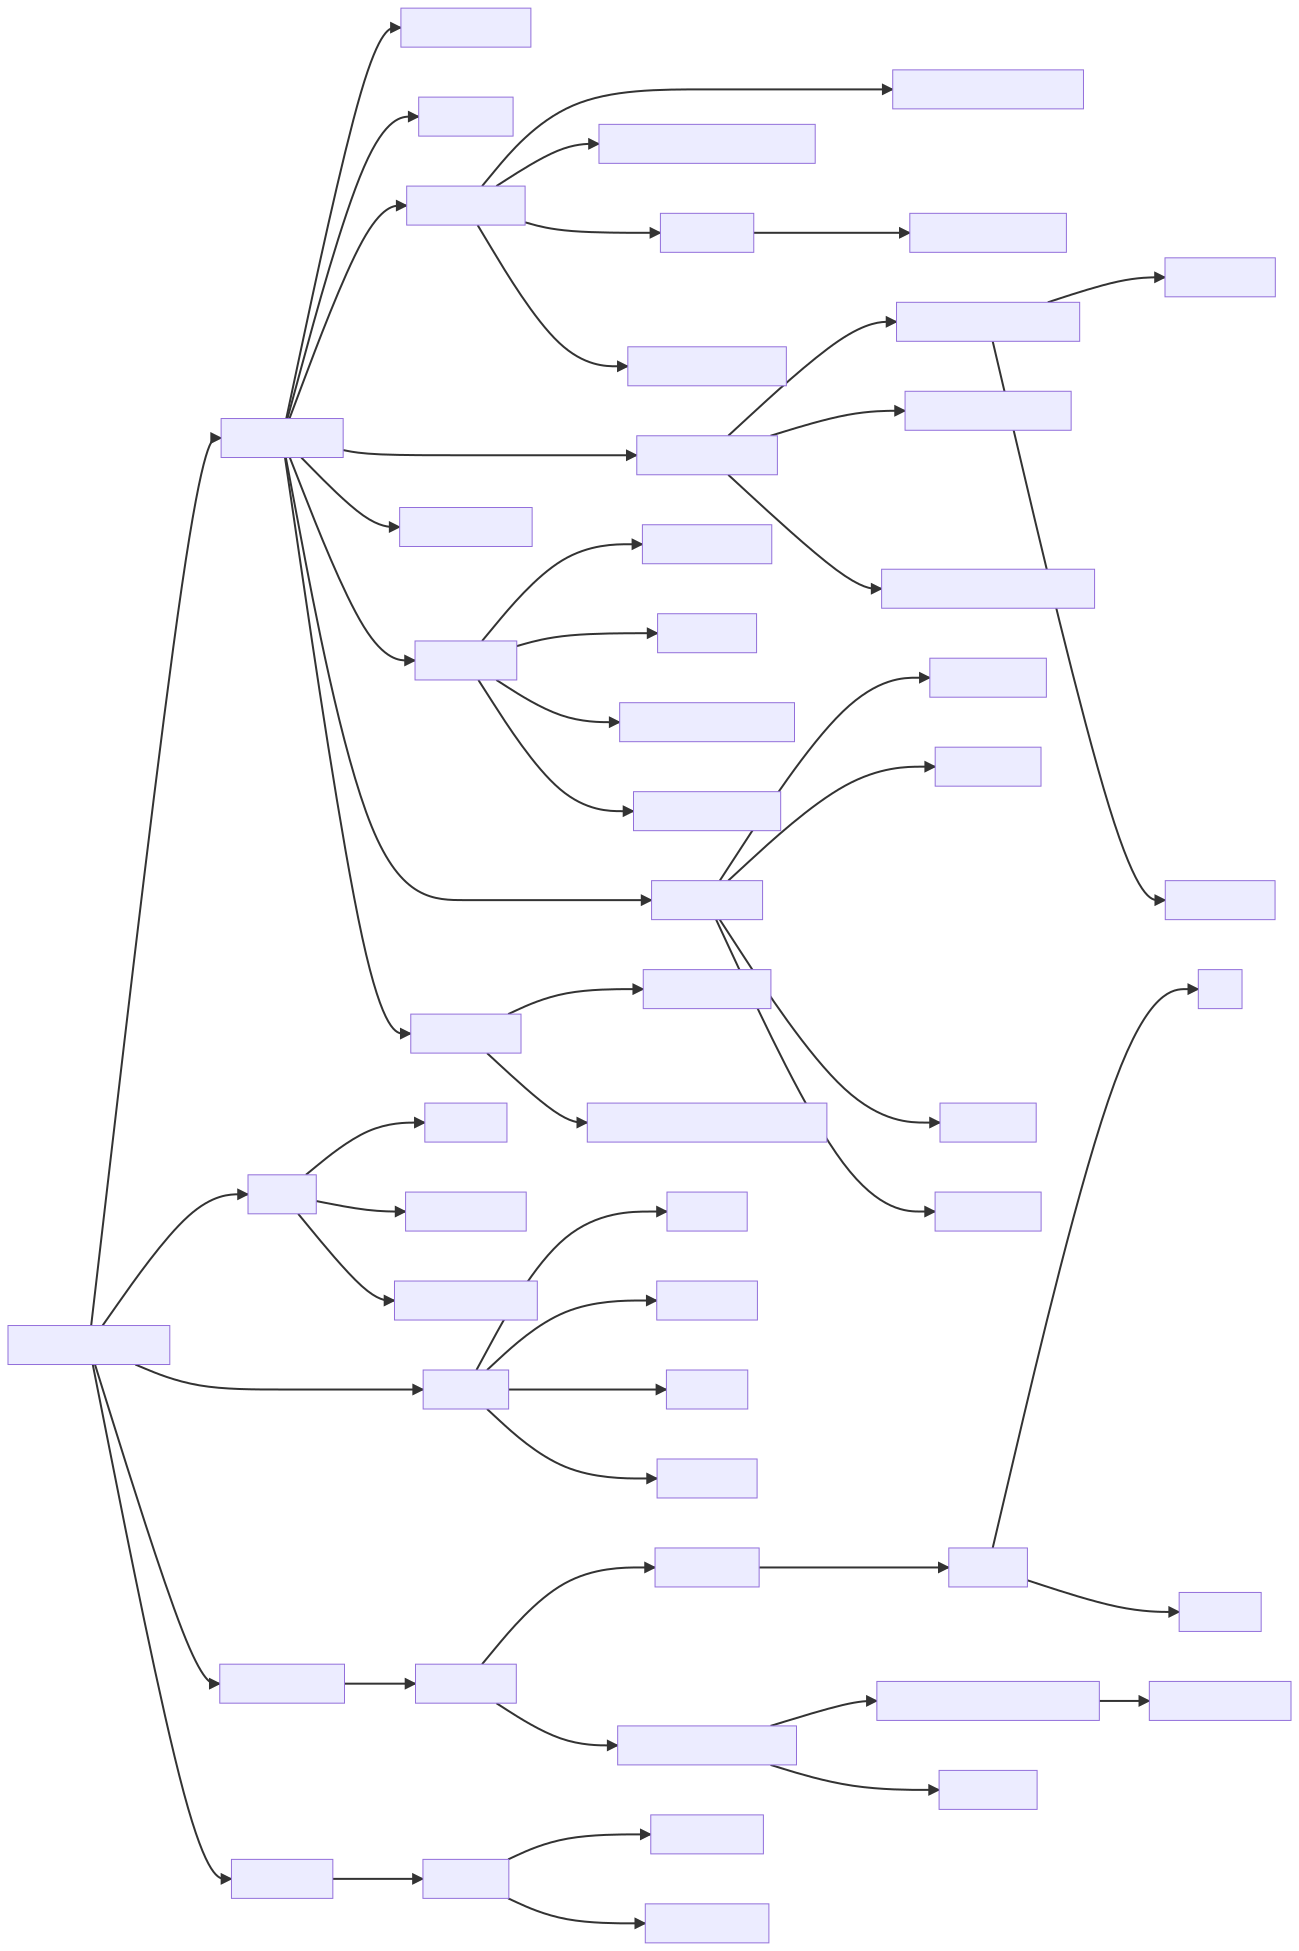
\includepdf[pages=-]{graphs/decomposition-design.pdf}

\subsection{NavigationView}
\label{sec:NavigationViewDesign}

\includegraphics[width=\textwidth, height=\textheight, keepaspectratio]{NavigationView-design}

The NavigationView provides a global menu for the user to navigate between different pages in the software. There are six tabs in the NavigationView, ``Home'', ``Problems'', ``Assignments'', ``Playground'', ``Account'', ``Settings''. By clicking on a different tab, the mainframe will display the corresponding page. The currently selected tab will be highlighted.

\subsubsection{Usability feature}

The entire NavigationView is a usability feature. Users can always look it up by clicking the top left button. They will be able to know where they are and navigate to other pages with one click, which makes the program easier to use.

\subsubsection{Validation}

There are only buttons in the NavigationView for the user to click, so only valid actions can be taken, no further data validation is required.

\subsection{HomePage}
\label{sec:HomePageDesign}

\includegraphics[width=\textwidth, height=\textheight, keepaspectratio]{HomePage-design}

The HomePage is the first page that gets displayed to the user. On the top of the HomePage, there will be a beautiful background image under the `Algorithm Dynamics' title. On the bottom, there are 10 useful buttons link to different functions.

\subsubsection{Usability feature}

The `Random' button starts a random problem for the user. The `Import' button calls the system file explorer for the user to import problems, problem lists, or assignments. The `Playground', `Problems', `Assignments' and `Account' button links the user to the corresponding page. The three buttons at the end link to three useful websites, when users click the button, the default web browser will be called and directed to these websites, which makes it easy for the user to look up specifications and revise content. All the useful functions of the software are grouped on the HomePage, which makes them easily accessible and makes the software easy to use.

\subsubsection{Validation}

There are only buttons in the HomePage for the user to click, so only valid actions can be taken, no further data validation is required.

\subsubsection{Stakeholder feedback}
\label{subsubsec:homepage stakeholder feedback}

Timofei thinks putting the links on the same page makes it messy. He thinks those websites and resources can be easily found on the Internet, so there is no need to put extra links on the HomePage.

PCloud points out that the icon grid needs to be responsive, so when he uses the software on a small screen, all buttons should still be displayed properly.

Mr Grimwood says it will be great if some greeting messages with recommendations can be displayed, such as ``You have 6 assignments to do this week.'' or ``You did pretty bad on data structures problems last time, maybe try this problem list to help you revise better.''

\subsubsection{Response}

Timofei has a good point here, and I decide to remove these links. The UI will be responsive to different window sizes, and this will be tested.

The greeting message and recommendations is a great idea. I will add an additional row below the image to display the greeting and recommendations.

\includegraphics[width=\textwidth, height=\textheight, keepaspectratio]{HomePage-Updated-design}

This is the redesigned HomePage. It adds greeting messages and recommendations. It has a responsive grid and a scroller is displayed when the item does not fit in one page. The useless links are removed.

\subsection{ProblemsPage}
\label{sec:ProblemsPageDesign}


\includegraphics[width=\textwidth, height=\textheight, keepaspectratio]{ProblemsPage-design}

The ProblemsPage displays all problems in the database. The user can search, create, edit, delete, import, export or start working on one or multiple problems on this page.

\subsubsection{Usability feature}

The user can apply the selection condition by either selecting different fields in the dropdown boxes or directly typing into the search box. A scrollable list of problems that match the conditions will be shown below with detailed information. The user can start working on a problem by clicking the start button on the right. They can also right-click the problem to call a context menu that includes more actions for them to delete, edit or export the problem. By clicking the select button on the top, the user can select multiple problems at once and apply the same action to them at once. By clicking the Add button on the top right, a context menu will be displayed, allowing the user to create or import new problems or problem lists. When the user is typing into the search box, a flyout will display matching results to save typing. I will implement an advanced searching algorithm to improve the quality of the search results, and I will explain the algorithm in the \hyperref[sec:algorithm design]{algorithm design section}.

\subsubsection{Validation}

Most components on this page are still buttons, users can only click them and no invalid data can be input. The search box is where the user can input some text only. A flyout will be displayed to promote the user to click the button instead of inputting data themselves. Also, a length check will be applied. The user can only enter a maximum of 32 characters so they cannot crash the search box or the searching algorithm. Instead of passing the search keywords directly to the database, a custom searching algorithm will be used to search and sanitise the search keyword, which prevents SQL injection and provide a better searching experience.

\subsection{CodingPage}
\label{sec:CodingPageDesign}

\includegraphics[width=\textwidth, height=\textheight, keepaspectratio]{CodingPage-design}

The CodingPage is where the user works on a programming problem. It contains a question panel, a code editor and an IO panel.

\subsubsection{Usability feature}

The question is displayed on the left and a code editor will be displayed on the top right. The input, output and error messages will be displayed on the button right, the user can switch between them by clicking the corresponding tab. On the bottom, the user can select programming language using a dropdown menu, run code by clicking the run code button and submit their code for judging by clicking the submit button. The status field shows the status of the judger and 3 navigation buttons on the button right to make it easy to navigate between different problems. There is a progress bar between the IO panel and the navigation buttons, it displays the judging progress.

The code editor will support line numbers, basic syntax highlighting and keyboard shortcuts to make it easy to use.

\subsubsection{Validaton}

Again, most of the components on the page are either read-only (such as the question section) or buttons. The code editor is the only place for the user to input text, and the text inside will be validated by the compiler or the interpreter of the selected programming language. However, the IO panel requires further validation. To prevent the user from printing out a huge amount of data which might result in poor performance, the IO panel will perform a length check and only display the first 2048 characters of the output.

\subsection{AssignmentsPage}
\label{sec:AssignmentsPageDesign}

\includegraphics[width=\textwidth, height=\textheight, keepaspectratio]{AssignmentsPage-design}

The AssignmentsPage is where the user interacts with the assignments. For students, they can work on their assignments; for teachers, they can create and mark assignments.

\subsubsection{Usability feature}

The user can switch between different tabs by clicking the navigation bar at the top. They can enter the detailed view of an assignment by clicking one assignment. A dropdown button is placed on the top right for the user to create or import a new assignment. All assignments will be displayed in a list with their due date.

\subsubsection{Validation}

There are only buttons for the user to click, so only valid actions can be taken, no further data validation is required.

\includegraphics[width=\textwidth, height=\textheight, keepaspectratio]{AssignmentsStudentDetailsPage-design}

This is the assignment details page for students, which gets displayed when a student clicks on an assignment.

\subsubsection{Usability feature}

The descriptions and due date of the assignment are displayed on the top left. A list of problems is displayed below where the user can see their status and start working on one by clicking it. When the user clicks the start button, he will be navigated to the CodingPage and the problems will be loaded. When he finishes all problems, he can click the submit button to either submit it through API or export it to a file to send to the teacher for marking.

\subsubsection{Validation}

There are only buttons for the user to click, so only valid actions can be taken, no further data validation is required.

\includegraphics[width=\textwidth, height=\textheight, keepaspectratio]{AssignmentsTeacherDetailsPage-design}

This is the assignment details page for teachers, which gets displayed when a teacher clicks on an assignment.

\subsubsection{Usability feature}

The teacher can click the Import Submissions button to import students' submissions or click the edit button to edit the assignment, or the export button to distribute the assignment. All student submissions and their status will be listed on the right, the teacher can click the mark button to mark all of them automatically and click the student submission to see the code details in the CodeingPage.

After marking, the teacher can click the export results button to export all student's marks into a CSV file for further data analysis.

\subsubsection{Validation}

There are only buttons for the user to click, so only valid actions can be taken, no further data validation is required.

\subsection{PlaygroundPage}
\label{sec:PlaygroundPageDesign}

\includegraphics[width=\textwidth, height=\textheight, keepaspectratio]{PlaygroundPage-design}

The PlaygroundPage is a free space for the user to run any code quickly. It is essentially the same page as the CodingPage but without a coding problem. The interface is slightly changed with a larger code editor and a separate IO panel for a better user experience.

\subsection{AccountPage}
\label{sec:AccountPageDesign}

\includegraphics[width=\textwidth, height=\textheight, keepaspectratio]{AccountPage-design}

The AccountPage is used to manage the current user and display user statistics.

\subsubsection{Usability feature}

If the user has login into his Microsoft account, the avatar, username, email and role will be managed by his Microsoft Account, the edit button will navigate to the Microsoft account website, and the login button will be replaced with a logout button. If the user has a login locally, he can edit his information by clicking the edit button and log in to Microsoft account by clicking the login button.

Some interesting statistics will be displayed on the button.

\subsubsection{Validation}

When the user edits his local identity, the user name will not be allowed to exceed 32 characters, and a format check will be applied to the email address.

\subsubsection{Stakeholder feedback}
\label{subsubsec:accountpage stakeholder feedback}

Timofei thinks there can be more interesting statistics, such as favourite variable names, and the total time spends in the software.

Mr Grimwood suggests that ``topic needs more revision'' can be added to the statistics.

\subsubsection{Response}
It may be too difficult to implement such statistics but this is an interesting idea. This feature is put in the backlog and will not be implemented for now.

``Topic needs more revision'' will be put as a recommendation, on the HomePage instead, which will make it more useful.

\subsection{SettingsPage}
\label{sec:SettingsPageDesign}

\includegraphics[width=\textwidth, height=\textheight, keepaspectratio]{SettingsPage-design}

The SettingsPage is where the user adjusts software settings.

\subsubsection{Usability feature}

The user can adjust the colour theme of the software to use a light theme, dark theme or system default theme. The user can also change the run code time limit, memory limit and programming language profiles in the SettingsPage.

\subsubsection{Validation}

Radio buttons are used for colour theme selection so it is impossible to enter any invalid data. A number box is used for the time limit and memory limit settings so only positive integers can be input. A dropdown list is used for the programming language setting so only valid input is accepted.

\subsubsection{Stakeholder feedback}
\label{subsubsec:settingspage stakeholder feedback}

Timofei likes the idea of being able to switch between a light theme and a dark theme. He thinks it will be better if users are allowed to create their custom themes. He also suggests that allowing the user to change the font size manually may help a lot.

\subsubsection{Response}

Extra themes take too much time to design, but it is an interesting idea. The font size is managed by the system and it is not very easy to change. Both ideas are great, they are put into the backlog and will not be implemented right away.

\subsection{CreateNewProblemPage}
\label{sec:CreateNewProblemPageDesign}

\includegraphics[width=\textwidth, height=\textheight, keepaspectratio]{CreateNewProblemPage-design}

The CreateNewProblemPage is used to create new problems. It contains multiple text boxes for the user to input problem information.

This page will be reused for editing existing problems. The title will be altered correspondingly.

\subsubsection{Usability feature}

The Tags field will be a tokenizing text box with an auto suggestion dropdown menu to make input faster. The Difficulty field will have a dropdown list for easy selection. The Time Limit and Memory Limit fields will be number boxes. The user can add a new test case by clicking the add button and removing existing ones by clicking the delete button. If the user clicks the cancel button, a flyout will be displayed to confirm cancellation.

\subsubsection{Validation}

There are many input boxes on this page, they will all be validated. For the Problem Name field, the user can enter 32 characters at maximum. In the Tags field, the user can enter 5 tags at maximum. In the Time Limit and Memory Limit fields, the user can only enter numbers.

\subsection{CreateNewProblemListPage}
\label{sec:CreateNewProblemListPageDesign}

\includegraphics[width=\textwidth, height=\textheight, keepaspectratio]{CreateNewProblemListPage-design}

The CreateNewProblemListPage is used to create a new problem list. It contains multiple text boxes for the user to input problem list information.

The page will be reused for editing existing problem lists. The title will be altered correspondingly.

\subsubsection{Usability feature}

There will be an autosuggest box for the user to search for problems and add them to the list. There is an export and a save button at the button for the user to export or save the problem list. If the user clicks the cancel button, a flyout will be displayed to confirm cancellation. The test cases will be a scrollable list to display multiple test cases.

\subsubsection{Validation}

A similar validation is performed just like the CreateNewProblempage. For the List Name field, the user can enter 32 characters at maximum.

\subsection{CreateNewAssignmentsPage}
\label{sec:CreateNewAssignmentsPageDesign}

\includegraphics[width=\textwidth, height=\textheight, keepaspectratio]{CreateNewAssignmentsPage-design}

The CreateNewAssignmentsPage is used to create new assignments. It contains multiple text boxes for the user to input assignment data.

The page will be reused for editing existing assignments as well. The title will be altered correspondingly.

\subsubsection{Usability feature}

The due date will be a DateTime picker, a visual calendar will be displayed for the user to pick a due date. An autosuggest search box will be placed for the user to search for problems easily.

\subsubsection{Validation}

The DateTime picker will prevent invalid dates from being input, the name field will have a maximum of 32 characters limit.

\subsection{Judger module}

The Judger module will handle all the judging and marking tasks. It takes in a \code{Submission}, compile and execute the user's code, judges whether it gives the correct output.

The Judger will take a few seconds to judge each \code{Submission}, while it is judging, the other parts of the software need to keep working on their tasks. So I use concurrent processing to let the Judger run parallel with the main program.

When judging a single \code{TestCase}, the Judger will first start the compiler in a new process to compile the user's code. The Judger redirects the output of the compiler to an internal string variable to store all outputs. When the compiler finishes compiling, an interrupt is triggered and the Judger will be notified that the compilation has been done. It will check the compiler's exit code and its output, if there are any compilation errors, they will be reported back. Otherwise, the Judger will run the compiled executable, and feed the input to its \code{stdin} and redirects all \code{stdout} and \code{stderr} to internal string variables. On top of that, the Judger will start a countdown timer in a different process to track the time. When the countdown reaches zero, an interrupt will be sent to the Judger and it will terminate the user's code and report a time limit exceed error, or if the user's code finishes first, then its output will be compared with the expected output, the result and all statistics will then be reported.

A problem may contain multiple test cases, so all test cases will be first pushed into a judging queue, and the judger will judge them one by one.

Similarly, an assignment may contain multiple problems, all problems will be first pushed into a problem queue, and each problem will be processed one by one.

The detailed judging algorithm will be explained later in the 
\hyperref[sec:algorithm design]{algorithm design section}.

\subsection{Database module}

Because this software will store many complex relational data, a relational database is needed to store all the data. Since the software runs locally, and every user will have different data, instead of a central SQL Server, a local SQL Database engine is required.

I choose to use SQLite to power this software. It is a small, self-contained, high-reliability, full-featured SQL Database engine, which will be enough to handle all the data storing and querying requests.

The SQLite database has some limitations. It only supports five data types. \code{TEXT}, \code{INTEGER}, \code{NULL}, \code{REAL} and \code{BLOB}. So other data types such as \code{DateTime} and \code{Guid} will need to be converted before storing.

I choose to use Microsoft.Data.SQLite for the database interface, which allows me to send SQL requests to the database, handle errors and provide safety features to prevent SQL injection. Details about the design of the database and queries will be described in the \hyperref[subsec:database design]{Database design section}.

\subsection{API module}

The API module will allow the user to log in to their Microsoft Education account, and interact with the Education Assignment function. Users will be able to create and manage assignments using education assignments APIs provided by Microsoft.

When the user clicks the login button in the SettingsPage, the API module will handle the login requests. When a logged-in user opens the AssignmentsPage, the API module will fetch all assignments. The API module will also allow the teachers to distribute assignments directly through API calls and the students to hand in submissions without any kind of exporting.

The API module will be implemented at the end after all local functions are working correctly. The corresponding API calls and endpoints will be discussed later.

\subsection{Stakeholder feedback}

I conduct an interview with each stakeholder after designing all the user interface elements. The statkeholders are generally very satisfying with the design. Suggestions are mainly about the \hyperref[subsubsec:homepage stakeholder feedback]{HomePage design} and the \hyperref[subsubsec:accountpage stakeholder feedback]{AccountPage design}, I have recorded their suggestions and my responses in those sections.

\section{Algorithm design}
\label{sec:algorithm design}

\subsection{Searchbox searching algorithm}

This algorithm will be used to power all the search boxes in the software. It will be packed into a function, taking in a list of items and the searching keyword input by the user, returning a list of results. To make the software easy to use, instead of simply using a linear search and returning all matching results, the algorithm will perform some fuzzy searching, so even the word is not typed in completely, matching results will be returned.

\begin{minted}{text}
function search(sourceList, keyword)
    // Create an empty list to store the results
    resultList = new List<string>()
    // Split the keyword into pieces by space
    splitKeyword = keyword.ToLower().Split(' ')
    // Compare each piece of keyword with the sourceList
    // Add the matching result into resultList
    for i=0 to sourceList.Length - 1
        for j=0 to splitKeyword.Length - 1
        sourceKey = sourceList[i].ToLower()
            if sourceKey.Contains(splitKeyword[j]) then
                resultList.Add(sourceList[i])
            endif
        next j
    next i

    // If no result is found,
    // add an "not found" notice to the resultList
    if resultList.Length == 0 then
          resultList.Add("No results found")
    endif
endfunction
\end{minted}

In this algorithm, I first create an empty list to store the result. Then I split the keyword into a list by space. So the keyword ``A Long Problem Name'' will be splitted into \code{["A", "Long", "Problem", "Name"]}.

Next, I use two nested loops to perform a linear search on each keyword. I choose to use the linear search here because the list is not sorted, so only it will work. The overall time complexity here is $O(nm)$ where $n$ is the length of the \code{sourceList} and $m$ is the length of \code{splitKeyword}. This is not very fast, but in real-world use cases, both $n$ and $m$ will be very small (less than 1000), so this algorithm will be fast enough to handle most of the cases. The increase in complexity brings a better searching experience. In this way, the algorithm will be able to match keywords like ``prob'' to result in ``A Long Problem List'', while normal linear search will not be able to do this.

In the end, if no item is found, a not found notice is added to the list, which will be displayed to the user.

\subsection{Judger RunCode algorithm}

This algorithm is designed for the Judger to run a piece of code, pass input to the code and receive all the output and error. This is the basic function of the Judger and further judging will all base on this algorithm.

Before anything can run, the Judger will need to first write the user's code to a source code file. And before it can do that, it needs to know where it should write to. I will create three private variables \code{_SourceCodeFilePath}, \code{_SourceCodeFolderPath} and \code{_ExecutableFilePath} to store the file paths for the source code file and the executable file. I use the idea of encapsulation here so these variables can only be set by the public method \code{SetSourceCodeFilePath}, so they will not be modified unexpectedly.

\begin{minted}{text}
partial class Judger
    private _SourceCodeFilePath
    private _SourceCodeFolderPath
    private _ExecutableFilePath

    public procedure SetSourceCodeFilePath(FolderPath, FileName)
        _SourceCodeFolderPath = FolderPath
        _SourceCodeFilePath = FolderPath + FileName + ".txt"
        _ExecutableFilePath = FolderPath + FilePath + ".exe"
    endprocedure
endclass
\end{minted}

For compiling programming languages such as C, C++ and Java, the source code needs to be compiled before running. So I need to add a \code{Compile} function to support these programming languages. The compile task needs to be run concurrently in a different process so the main UI can stay responsive. So instead of monitoring the compiler all the time, I will bind two event handlers to the compile process, to process its output data and error data. Those data will then be stored in two private string variables for later use.

\begin{minted}{text}
partial class Judger
    private _CompilationOutput
    private _CompilationError

    private procedure CompileProcess_ErrorDataReceived(sender, e)
        // Validate the data before storing
        if string.IsNullOrEmpty(e.Data) == False then
            _CompilationError += e.Data + '\n'
        endif
    endprocedure

    private procedure CompileProcess_OutputDataReceived(sender, e)
        // Validate the data before storing
        if string.IsNullOrEmpty(e.Data) == False then
            _CompilationOutput += e.Data + '\n
        endif
    endprocedure
endclass
\end{minted}

Now, it is ready to run the compiler. Before it can start compiling, the old outputs need to be cleaned. I design two magic variables in the language configurations allowing more flexible arguments, these magic variables need to be pre-processed before compiling. A process start info needs to be created to let the Judger know how to start the new process. After binding the event handlers, the compiler can start running.

\begin{minted}{text}
partial class Judger
    private function Compile()
        // Clear the old data
        _CompilationOutput = ""
        _CompilationError = ""

        // Pre-process language compile command and arguments
        string fileName = language.CompileCommand.Replace("{SourceCodeFilePath}", _SourceCodeFilePath).Replace("{ExecutableFilePath}", _ExecutableFilePath)
        string arguments = language.CompileArguments.Replace("{SourceCodeFilePath}", _SourceCodeFilePath).Replace("{ExecutableFilePath}", _ExecutableFilePath)
        
        // Create a new process start info
        ProcessStartInfo StartInfo = new ProcessStartInfo
        (
            FileName: fileName,
            Arguments: arguments,
            UseShellExecute: false,
            CreateNoWindow: true,
            RedirectStandardOutput: true,
            RedirectStandardError: true,
        )
        
        // Create a new compile process
        Process CompileProcess = new Process(StartInfo)
        
        // Bind event handlers to the compile process
        CompileProcess.OutputDataReceived += new DataReceivedEventHandler(CompileProcess_OutputDataReceived)
        CompileProcess.ErrorDataReceived += new DataReceivedEventHandler(CompileProcess_ErrorDataReceived)
        
        // Start the compile process
        CompileProcess.Start()
        CompileProcess.BeginOutputReadLine()
        CompileProcess.BeginErrorReadLine()
        CompileProcess.WaitForExitAsync()

        // Return the exit code
        return CompileProcess.ExitCode
    endfunction
endclass
\end{minted}

In the end, an integer exit code will be returned. If the exit code is zero, the Judger will know that the compilation is successful. If it is something else, then the Judger will need to report a compile error with detailed data from \code{_CompilationError}. 

If the user's code is compiled successfully or it does not need to be compiled, the \code{Execute} function is called to run the code or the executable, pass the input to the process and get its output. The \code{Execute} function will also need to kill the running process if it runs too long. So I will use a custom enumeration type \code{StatusCode} to manage the process' status.

\begin{minted}{text}
enum StatusCode
    PENDING,
    RUNNING,
    FINISHED,
    TIME_LIMIT_EXCEEDED,
    MEMORY_LIMIT_EXCEED
endenum

partial class Judger
    private _StatusCode
endclass
\end{minted}

\code{StatusCode} has five possible values, \code{PENDING} is set when the code is waiting to be run. When it starts executing, the status code will be set to \code{RUNNING}. If it finishes in time, its status will be set to \code{FINISHED}. If it exceeds the time limit, the process will be killed by the Judger and a \code{TLE} will be recorded. If it exceeds the memory limit, the process will be killed by the Judger and a \code{MLE} will be recorded.

Similarly, I will use event handlers to record all the outputs from the user's code. I add a third handler to process the exit event, which will determine the \code{_StatusCode} mentioned above.

\begin{minted}{text}
partial class Judger
    private _StandardOutput
    private _StandardError

    private procedure ExecuteProcess_Exited(sender, e)
        // Only successfully finished when the status code is not TLE or MLE
        if _StatusCode != StatusCode.TIME_LIMIT_EXCEEDED and _StatusCode != StatusCode.MEMORY_LIMIT_EXCEED then
            _StatusCode = StatusCode.FINISHED
        endif
    endprocedure

    private procedure ExecuteProcess_OutputDataReceived(sender, e)
        // Validate the data before storing
        if string.IsNullOrEmpty(e.Data) == False then
            _StandardOutput += e.Data + '\n'
        endif
    endprocedure

    private procedure ExecuteProcess_ErrorDataReceived(sender, e)
        // Validate the data before storing
        if string.IsNullOrEmpty(e.Data) == False then
            _StandardError += e.Data + '\n'
        endif
    endprocedure
endclass
\end{minted}

The \code{Execute} function has a similar design with the \code{Compile} function. It configures all the running information and event handlers as usual. However, this time I add two extra processes running concurrently with the execution process. The first one is a timer, which countdown the time limit. When the timer counts to zero, it checks whether the execute process is still running, if it does, then the execution process will be killed and a \code{TLE} will be reported. The second one is a memory monitor, which checks the peak memory usage of the execution process every 10 milliseconds. If the memory usage is larger than the memory limit, then the execution process will be killed and a \code{MLE} will be reported.

\begin{minted}{text}
partial class Judger
    private _WorkingSet64;
    private function Execute(Input, Language, TimeLimit, MemoryLimit)
        // Clear the old data
        _StandardOutput = ""
        _StandardInput = ""
        _WorkingSet64 = 0

        // Initialize status code
        _StatusCode = StatusCode.PENDING

        // Pre-process language run command and arguments
        string fileName = Language.RunCommand.Replace("{SourceCodeFilePath}", _SourceCodeFilePath).Replace("{ExecutableFilePath}", _ExecutableFilePath)
        string arguments = Language.RunArguments.Replace("{SourceCodeFilePath}", _SourceCodeFilePath).Replace("{ExecutableFilePath}", _ExecutableFilePath)

        // Create a new process start info
        ProcessStartInfo StartInfo = new ProcessStartInfo
        (
            FileName: fileName,
            Arguments: arguments,
            UseShellExecute: false,
            CreateNoWindow: true,
            RedirectStandardInput: true,
            RedirectStandardOutput: true,
            RedirectStandardError: true,
        )

        // Create a new execute process
        Process ExecuteProcess = new ExecuteProcess(StartInfo)

        // Bind event handlers to the compile process
        ExecuteProcess.OutputDataReceived += new DataReceivedEventHandler(ExecuteProcess_OutputDataReceived)
        ExecuteProcess.ErrorDataReceived += new DataReceivedEventHandler(ExecuteProcess_ErrorDataReceived)
        ExecuteProcess.Exited += new EventHandler(ExecuteProcess_Exited)
        
        // Start the execute process
        ExecuteProcess.Start()
        ExecuteProcess.BeginOutputReadLine()
        ExecuteProcess.BeginErrorReadLine()
        ExecuteProcess.StandardInput.WriteLine(Input);

        // Set the status code to Running
        _StatusCode = StatusCode.RUNNING
        
       // Start the timer
        Timer timer = new Timer(() => 
        {
            // If the user's code is still running 
            // when the timer has finished
            // Kill the user's code and record a TLE
            if ExecuteProcess.HasExited == false then
                ExecuteProcess.Kill()
                _StatusCode = StatusCode.TIME_LIMIT_EXCEEDED
            endif
        }, null, TimeLimit, Timeout.Infinite)

        // Start the memory monitor
        Thread MemoryMonitor = new Thread(() =>
        {
            while ExecuteProcess.HasExited == false
                ExecuteProcess.Refresh()
                _WorkingSet64 = ExecuteProcess.PeakWorkingSet64
                if _WorkingSet64 > MemoryLimit then
                    ExecuteProcess.Kill()
                    _StatusCode = StatusCode.MEMORY_LIMIT_EXCEEDED
                endif
            endwhile
        });
        MemoryMonitor.Start()

        // Wait the process to finish
        ExecuteProcess.WaitForExitAsync()

        // Return the exit code
        return ExecuteProcess.ExitCode
    endfunction
endclass
\end{minted}

Now I have everything I need to build the \code{RunCode} function. It takes in the user's code, input data, language configuration, time limit and memory limit, outputs a \code{RunCodeResult} containing all the running information. I also need to set up a stopwatch to measure how long the code has been executed, unlike the timer before, this stopwatch only provides data for statistics records. In the end, the \code{RunCode} function will handle some basic errors, it will judge whether the user's code run, but it will not judge whether the user's code provides the correct output. The \code{RunCode} algorithm only runs the code and further judging will be handed over to other algorithms.

\begin{minted}{text}
partial class Judger
    public function RunCode(UserCode, Input, Language, TimeLimit, MemoryLimit)
        // Create a new TestCaseResult
        RunCodeResult result = new RunCodeResult()

        // Write the source code to file
        sourceCodeFile = openWrite(_SourceCodeFilePath)
        sourceCodeFile.write(UserCode)
        sourceCodeFile.close()

        // Compile if needed
        if Language.NeedCompile then
            // Compile and record the exit code
            exitCode = Compile(Language)

            // If compile failed then return a COMPILE_ERROR
            if exitCode != 0 then
                result.StandardOutput = _CompilationOutput
                result.StandardError = _CompilationError
                result.ResultCode = ResultCode.COMPILE_ERROR
                return result
            endif
        endif

        // Set up a Stopwatch to record the running time
        Stopwatch watch = new Stopwatch()
        watch.Start()

        // Execute the code
        exitCode = Execute(Input, Language, TimeLimit)

        watch.Stop()

        // Store the stats to the result
        result.StandardOutput = _StandardOutput
        result.StandardError = _StandardError
        result.CPUTime = watch.ElapsedMilliseconds

        // If time limit exceed, return TLE
        if _StatusCode == StatusCode.TIME_LIMIT_EXCEEDED then
            result.ResultCode = ResultCode.TIME_LIMIT_EXCEEDED
            return result
        endif

        // If memory limit exceed, return MLE
        if _StatusCode == StatusCode.MEMORY_LIMIT_EXCEEDED then
            result.ResultCode = ResultCode.MEMORY_LIMIT_EXCEEDED
            return result
        endif

        // If receive a error or exit code is not zero
        // Return a runtime error
        if string.IsNullOrEmpty(result.StandardError) == False or exitCode != 0 then
            result.ResultCode = ResultCode.RUNTIME_ERROR
            return result
        endif

        // Otherwise, return success
        result.ResultCode = ResultCode.SUCCESS
        return result
    endfunction
endclass
\end{minted}

\subsection{Judger Judge TestCase algorithm}

This algorithm is designed to allow the Judger to judge a test case. On top of the \code{RunCode} function, this algorithm compare the user's output with the expected output, so it can judge whether the user's code works correctly. The \code{JudgeTestCase} function returns a \code{TestCaseResult} containing more information.

\begin{minted}{text}
partial class Judger
    public function JudgeTestCase(UserCode, TestCase, Language, TimeLimit)
        // Run the code with RunCode and get the result
        TestCaseResult result = (TestCaseResult)RunCode(UserCode, TestCase.Input, Language, TimeLimit)
        result.TestCase = TestCase

        // If the code is executed successfully
        // Judge whether its output matches the expected output
        if result.ResultCode == ResultCode.SUCCESS then

            // Trim the trailing spaces before comparing
            userOutput = result.StandardOutput.Trim()
            expectedOutput = TestCase.Output.Trim()

            // If they are not matched
            // Report wrong answer
            if userOutput != expectedOutput then
                result.ResultCode = ResultCode.WRONG_ANSWER
            endif
        endif
        return result
    endfunction
endclass  
\end{minted}

\subsection{Judger Judge Problem algorithm}

This algorithm is designed to judge a submission. I set up a judging queue and push all test cases into the queue. Then I take them out and judge them one by one. A queue is suitable for this use case because I want the first test case entered to be judged first. A submission result will be returned at the end.

\begin{minted}{text}
partial class Judger
    public function JudgeProblem(Submission)
        // Create the submission result
        SubmissionResult result = new SubmissionResult()
        result.Submission = Submission

        // Create the judging queue
        Queue JudgeQueue = new Queue(Submission.Problem.TestCases)

        // Keep judging until the queue is empty
        while len(JudgeQueue) > 0
            Code = Submission.Code
            TestCase = JudgeQueue.Dequeue()
            Language = Submission.Language
            TimeLimit = Submission.Problem.TimeLimit
            MemoryLimit = Submission.Problem.MemoryLimit
            TestCaseResult = JudgeTestCase(Code, TestCase, Language, TimeLimit, MemoryLimit)
            result.Add(TestCaseResult)
        endwhile
        return result
    endfunction
endclass
\end{minted}

\subsection{Judger Judge Assignment algorithm}

This algorithm is designed to judge an assignment submission. I set up a judging queue and push all problems into the queue. Then I take them out and judge them one by one. A queue is suitable for this use case because I want the first problem entered to be judged first. An assignment submission result will be returned at the end.

\begin{minted}{text}
partial class Judger
    public function JudgeAssignment(AssignmentSubmission)
        // Create the assignment submission result
        AssignmentSubmissionResult result = new AssignmentSubmissionResult()
        result.AssignmentSubmission = AssignmentSubmission

        // Create the judging queue
        Queue JudgeQueue = new Queue(AssignmentSubmission.Submissions)

        // Keep judging until the queue is empty
        while len(JudgeQueue) > 0
            Submission = JudgeQueue.Dequeue()
            SubmissionResult = JudgeProblem(Submission)
            result.Add(SubmissionResult)
        endwhile
        return result
    endfunction
endclass
\end{minted}

\section{Data structure design}

\subsection{Class design}

I am taking an object-oriented approach to the design of the software. This is the class diagram for all classes with their attributes and methods.

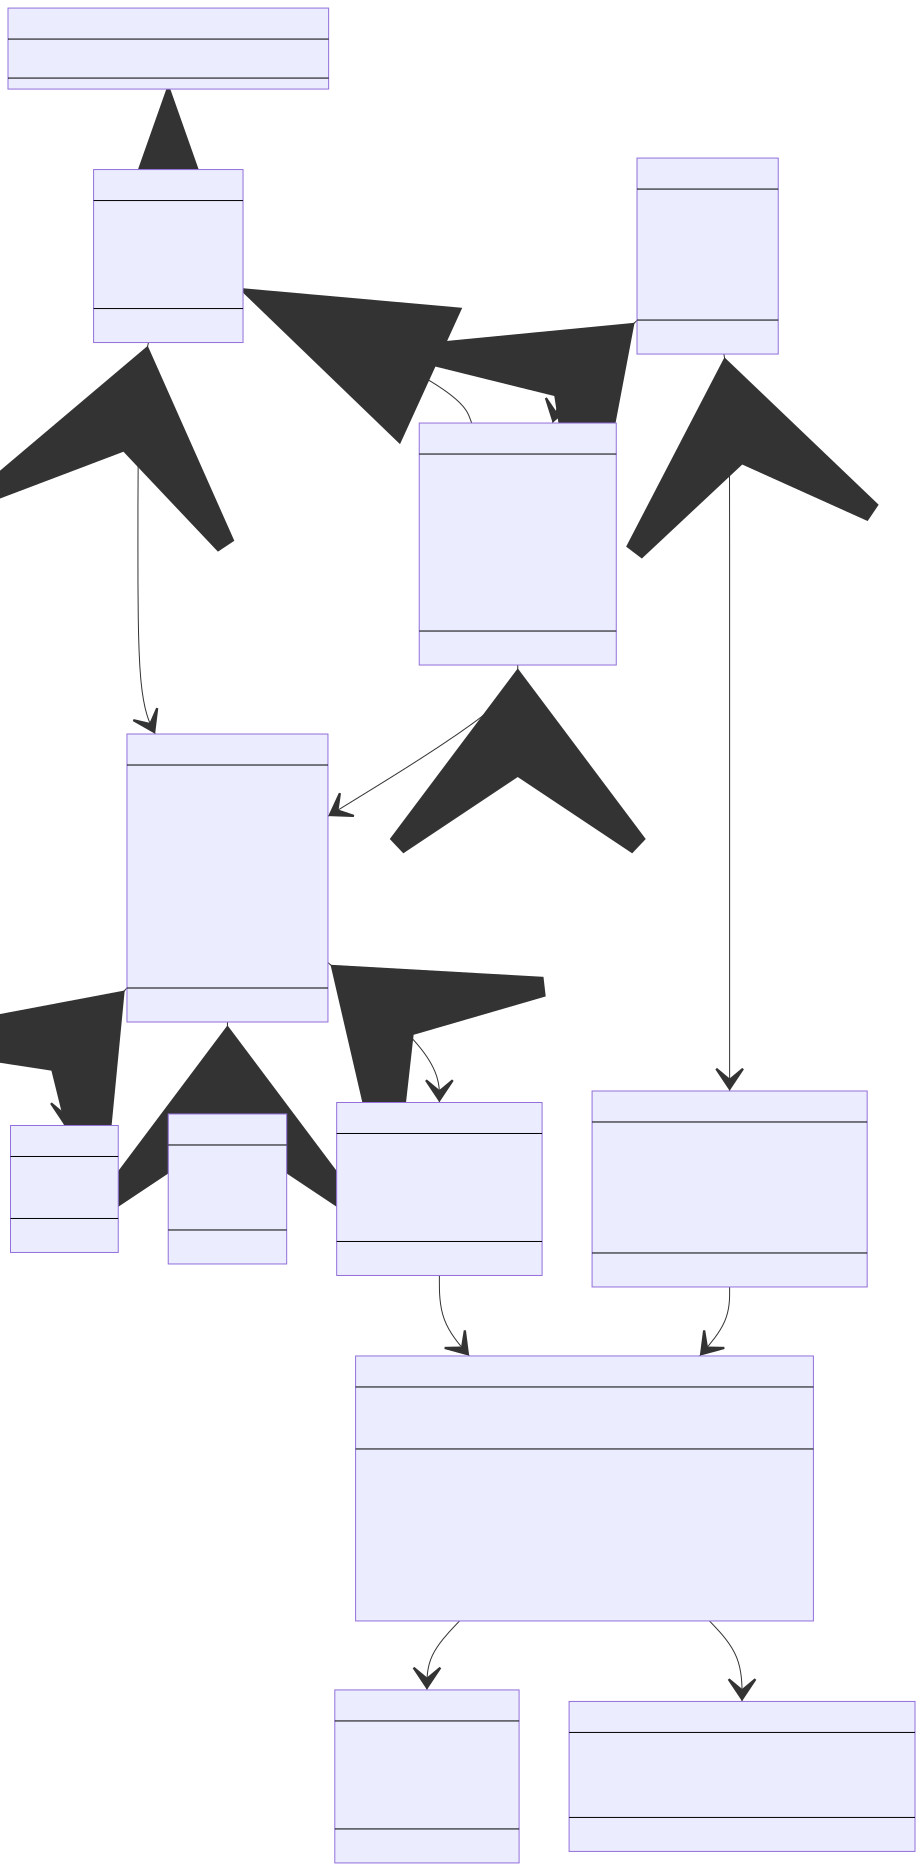
\includegraphics[width=\textwidth, height=\textheight, keepaspectratio]{classDiagram}

\subsubsection{User}

\code{User} is an object used to represent the current user. Its data will be attached to each \code{Submission}, \code{Assignment} and \code{AssignmentSubmission}, so the user can track identities and manage the data easily. Users will be asked to enter this information when they first open the software, an instance of \code{User} will be created and stored in the database.

\begin{tabulary}{\textwidth}{|l|l|L|}
    \hline
    Variable & Data type & Justification \\
    \hline
    \code{Uid} & \code{Guid} & The \code{User} uses a \code{Guid} value for its \code{Uid} instead of a normal \code{int} value to ensure the \code{Uid} is unique globally. Every user will have a unique \code{Uid}. \\
    \hline
    \code{Name} & \code{string} & \code{Name} stores the user's name. \\
    \hline
    \code{Email} & \code{string} & \code{Email} stores the user's Email address. \\
    \hline
    \code{Role} & \code{enum Role} & \code{Role} is a custom enumeration type which has two possible values, \code{Student} or \code{Teacher}. It is used to determine the role of the current user, and the user interface will be adjusted accordingly. I choose to use a custom enumeration type instead of some magic numbers to make the code more readable and easier to maintain. \\
    \hline
\end{tabulary}

\subsubsection{Tag}

A \code{Tag} is a label used to categorize a \code{Problem}.

\begin{tabulary}{\textwidth}{|l|l|L|}
    \hline
    Variable & Data type & Justification \\
    \hline
    \code{Id} & \code{int} & The \code{Id} is the local unique identifier for a \code{Tag}. It is used to uniquely determine a \code{Tag} in the local database. \\
    \hline
    \code{Name} & \code{string} & \code{Name} stores the name of the \code{Tag}. A \code{Name} must be unique, so data needs to be validated and two \code{Tags} with the same \code{Name} is not allowed. \\
    \hline
\end{tabulary}

\subsubsection{TestCase}

A \code{TestCase} is one set of test input and output, which will be used by the \code{Judger} to judge the user's submission.

\begin{tabulary}{\textwidth}{|l|l|L|}
    \hline
    Variable & Data type & Justification \\
    \hline
    \code{Id} & \code{int} & The \code{Id} is the local unique identifier for a \code{TestCase}. It is used to uniquely determine a \code{TestCase} in the database. \\
    \hline
    \code{Input} & \code{string} & The \code{Input} will be feed to the user's submission code by the \code{Judger}. \\
    \hline
    \code{Output} & \code{string} & \code{Output} stores the expected \code{Output} of the corresponding \code{Input}. The \code{Judger} will compare user's output with the \code{Output} to judge whether the user's code is correct. \\
    \hline
    \code{IsExample} & \code{bool} & Define whether this \code{TestCase} is an example. An example \code{TestCase} will be displayed to the user for debugging, and distribute with an \code{Assignment}. A non-example \code{TestCase} will be used to judge the solution and will not be displayed to the user or distribute with an \code{Assignment}. A boolean value is suitable to store the two-state data. \\
    \hline
\end{tabulary}

\subsubsection{Problem}

The \code{Problem} is used to store and organize the data for each programming question.

\begin{tabulary}{\textwidth}{|l|l|L|}
    \hline
    Variable & Data type & Justification \\
    \hline
    \code{Id} & \code{int} & The \code{Id} is the local unique identifier for a \code{Problem}. It is used to uniquely determine a \code{Problem} in the database. When a \code{Problem} is imported in to the database, a new \code{Id} is given. \\
    \hline
    \code{Name} & \code{string} & The \code{Name} is a string contains the name of a \code{Problem}. \\
    \hline
    \code{SourceHash} & \code{string} & This field is \code{null} for all normal \code{Problem}. It is only set for \code{Problem} which comes with an \code{Assignment}, and it is set to the hash value of the original \code{Problem}. This value will be recorded for \code{Submission}. \\
    \hline
\end{tabulary}

\begin{tabulary}{\textwidth}{|l|l|L|}
    \hline
    Variable & Data type & Justification \\
    \hline
    \code{Description} & \code{string} & The \code{Description} is a string storing the detailed description of a \code{Problem}. Markdown syntax is supported for a better user experience. \\
    \hline
    \code{Status} & \code{enum Status} & \code{Status} is an enumeration type containing 3 possible status: \code{Todo}, \code{Solved} and \code{Attempted}. This is used to collect user statistics data. I choose to use a custom enumeration type instead of some magic numbers to make the code more readable and easier to maintain. \\
    \hline
    \code{Difficulty} & \code{enum Difficulty} & \code{Difficulty} is an enumeration type containing 3 possible difficulties: \code{Easy}, \code{Medium} and \code{Hard}. This provdes a way for the user to search and select problems by their difficulties. \\
    \hline
    \code{TimeLimit} & \code{int} & \code{TimeLimit} sets the max time allowed for the user code to run in millisecond. When the running time exceed the \code{TimeLimit}, the running code will be killed and a Time Limit Exceed error will be recorded. This prevents infinite loop from using up all computing resources and rejects inefficient algorithms. \\
    \hline
    \code{MemoryLimit} & \code{int} & \code{MemoryLimit} sets the max memory allowed for the user's code to consume in bytes. When the memory usage exceed the memory limit, the running code will be killed and a Memory Limit Exceed Error will be recorded. This prevents incorrect code from using up all memory space and rejects inefficient algorithms. \\
    \hline
    \code{TestCases} & \code{List<TestCase>} & \code{TestCases} is a list containing all \code{TestCase} for the problem. A list is more appropriate than an array because it allows new \code{TestCase} to be added or remove existing ones during runtime. \\
    \hline
    \code{Tags} & \code{List<Tags>} & \code{Tags} is a list containing all \code{Tags} for a \code{Problem}. Similarly, I use a list for \code{Tags} so it can be added or removed during runtime. \\
    \hline
\end{tabulary}

\subsubsection{Language}

\code{Language} defines the compiling and running configurations for different programming languages. Language configurations are not stored in the database, instead, they are stored in the settings file, so users can add their custom configurations easily.

\begin{tabulary}{\textwidth}{|l|l|L|}
    \hline
    Variable & Data type & Justification \\
    \hline
    \code{Name} & \code{string} & \code{Name} stores the name of each programming language. The \code{Name} will be displayed in the drop down menu for the user to select their preferred programming language. \\
    \hline
    \code{NeedCompile} & \code{bool} & Some programming languages need to be compiled before running, such as C, C++ and Java. This attribute is used to tell the \code{Judger} to compile the code before executing. \\
    \hline
    \code{CompileCommand} & \code{string} & If a programming language requires compilation, this command is executed to call the compiler. \\
    \hline
    \code{CompileArguments} & \code{string} & If a programming language requires compilation, this arguments is passed to the compiler to specify file path and related compile arguments. \\
    \hline
    \code{RunCommand} & \code{string} & The \code{Judger} uses this command to run the executable or call the intrepreter. \\
    \hline
    \code{RunArguments} & \code{string} & This \code{Judger} pass this arguments to the executable or the intrepreter. \\
    \hline
\end{tabulary}

\subsubsection{Submission}

A \code{Submission} is created when the user submits a code solution to the \code{Judger}. The \code{Submission} will contain all the information including the time, the source code, the programming language selected and the corresponding \code{Problem} for the \code{Judger} to judge.

\begin{tabulary}{\textwidth}{|l|l|L|}
    \hline
    Variable & Data type & Justification \\
    \hline
    \code{Id} & \code{int} & The \code{Id} is the local unique identifier for a \code{Submission}. It is used to uniquely determine a \code{Submission} in the database. \\
    \hline
    \code{Problem} & \code{Problem} & The \code{Problem} contains the corresponding \code{Problem} of this \code{Submission}, which also contains the \code{TestCases} for the \code{Judger} to judge the \code{Submission}. Before storing a \code{Submission} into the database, this value needs to be normalized to the \code{Id} of that \code{Problem}. \\
    \hline
    \code{Code} & \code{string} & \code{Code} stores the submitted code, which will be executed and judged by the \code{Judger}. \\
    \hline
    \code{SubmittedTime} & \code{DateTime} & \code{SubmittedTime} stores the time the \code{Submission} is created. Instead of using a \code{string} or an \code{int} value, I decide to use the native data type \code{DateTime} provided by C\#, which makes it easier to process date time, and prevent any formating issues. \\
    \hline
    \code{Language} & \code{Language} & \code{Language} stores the programming language selected by the user, so the \code{Judger} knows how to run the code.\\
    \hline
    \code{Submitter} & \code{User} & \code{Submitter} stores the \code{User} who submits this \code{Submission}. This field will be normalized to the \code{User.Uid} before storing into the database. \\
    \hline
\end{tabulary}

\subsubsection{ProblemList}

A \code{ProblemList} is a list of \code{Problem}, which allows the user to share multiple \code{Problem} easily. It is also the parent of \code{Assignment} and provides basic functions for it. The \code{ProblemList} contains a \code{List<Problem>} variable, which provides all basic functions for a list, such as add, remove, sort and find, so I don't need to reinvent the wheel. I choose a list instead of an array because the number of \code{Problem} inside the list will be changed during runtime, so a list is more appropriate for my use case.

\begin{tabulary}{\textwidth}{|l|l|L|}
    \hline
    Variable & Data type & Justification \\
    \hline
    \code{Id} & \code{int} & The \code{Id} is the local unique identifier for a \code{ProblemList}. It is used to uniquely determine a \code{ProblemList} in the database. \\
    \hline
    \code{Name} & \code{string} & \code{Name} stores the name of the \code{Problem List}. \\
    \hline
    \code{Description} & \code{string} & \code{Description} stores the description of the \code{ProblemList}. \\
    \hline
    \code{Problems} & \code{List<Problem>} & \code{Problems} is a list of \code{Problem}, which supports basic functions to manipulate a list of data. \\
    \hline
\end{tabulary}

\subsubsection{Assignment}

An \code{Assignment} is a \code{ProblemList} which gets distributed to students. When an \code{Assignment} is distributed, a copy of that \code{Assignment} is created. All \code{TestCases} with \code{IsExample} set to \code{false} will be removed to prevent students from cheating. The \code{Type} of the \code{Assignment} will be set to \code{Copy} to indicate it is a distributed copy. The \code{Judger} will reject to judge a distributed \code{Assignment} and the \code{AssignmentsPage} will show the \code{Assignment} under the Assigned tab instead of the Created tab.

\code{Assignment} is inheriate from the \code{ProblemList}, so it can reuse the \code{Name} and \code{Description} attributes and all methods to manage a list of \code{Problem}. Upon that, new attributes and methods are added to make it functional.

\begin{tabulary}{\textwidth}{|l|l|L|}
    \hline
    Variable & Data type & Justification \\
    \hline
    \code{Uid} & \code{Guid} & The \code{Assignment} uses a \code{Guid} value for its \code{Uid} instead of a normal \code{int} value to ensure the \code{Uid} is unique globally. So when the user import an \code{Assignment} into their database, the \code{Uid} will not conflict with any existing values, and it will not be changed (Unlike a \code{ProblemList}, for which will be assigned a new \code{Id} when importing). The \code{Uid} will be referenced by the \code{AssignmentSubmission} so the \code{Judger} will be able to know which \code{Assignment} it is judging. \\
    \hline
    \code{DueDate} & \code{DateTime} & The \code{DueDate} stores the time for the due date of the \code{Assignment}. Instead of using a \code{string} or an \code{int} value, I decide to use the native data type \code{DateTime} provided by C\#, which makes it easier to process date time, and prevent all formating issues. \\
    \hline
    \code{Status} & \code{enum Status} & \code{Status} is an enumeration type containing 4 possible status for a source \code{Assignment}: \code{Draft}, \code{Scheduled}, \code{Published} and \code{Assigned} for the teacher to manage the lifecycle of an \code{Assignment}. For a distributed \code{Assignment}, there are 4 possible \code{Status}, \code{NotStarted}, \code{InProgress}, \code{Completed} and \code{OverDue}, which helps the student to manage the lifecycle of an \code{Assignment}. I choose to use a custom enumeration type instead of some magic numbers to make the code more readable and easier to maintain.\\
    \hline
    \code{Type} & \code{enum Type} & \code{Type} is an enumeration type containing 2 possible types, \code{Source} or \code{Copy}. It is used to manage the distribution of an \code{Assignment} as described above. \\
    \hline
    \code{Assigner} & \code{User} & \code{Assigner} stores the \code{User} who assigns the \code{Assignment}. This field will be normalized into the \code{User.Uid} before storing into the database. \\
    \hline
\end{tabulary}

\subsubsection{AssignmentSubmission}

When a student finishes an \code{Assignment}, an \code{AssignmentSubmission} is created for the \code{Judger} to judge. The \code{AssignmentSubmission} can either be exported to file and sent to the teacher, or it can be uploaded using API. The teacher imports the \code{AssignmentSubmission} or uses API to load it, and the \code{Judger} will be able to mark it and return the result.

\begin{tabulary}{\textwidth}{|l|l|L|}
    \hline
    Variable & Data type & Justification \\
    \hline
    \code{Uid} & \code{Guid} & The \code{AssignmentSubmission} uses a \code{Guid} value for its \code{Uid} instead of a normal \code{int} value to ensure the \code{Uid} is unique globally. So when teachers import an \code{AssignmentSubmission} into their database, the \code{Uid} will not conflict with any existing values, and it will not be changed. \\
    \hline
    \code{Submitter} & \code{User} & The user information is collected when exporting an \code{AssignmentSubmission}, so the teacher will be able to know who is the \code{Submitter}. This field needs to be normalized into \code{User.Uid} before storing into the database. \\
    \hline
    \code{Assignment} & \code{Assignment} & The \code{Assignment} corresponding to this \code{AssignmentSubmission} is recorded, so the \code{Judger} knows how to judge it. This field needs to be normalized into \code{Assignment.Uid} before storing into the database. \\
    \hline
    \code{Submissions} & \code{List<Submission>} & \code{Submissions} stores a list of \code{Submission}, which contains the user's \code{Submission} for each \code{Problem} assigned. \\
    \hline
    \code{Status} & \code{enum Status} & \code{Status} is an enumeration type containing 3 possible types, \code{NotJudged}, \code{Judged} and \code{Returned} for the teacher to keep track of each submission. \\
    \hline
\end{tabulary}

\subsubsection{Judger}

The \code{Judger} is a static class, only eposes 5 functions to run and judge user's code. The \code{Judger} takes a \code{Submission} as an input, and outputs a \code{SubmissionResult}. No variable is exposed. The private attributes and methods are discussed in the \hyperref[sec:algorithm design]{algorithm design section}.

\subsubsection{RunCodeResult}

\code{RunCodeResult} stores the judging result for a piece of code. It does not store the information about whether the output is correct, it only stores the runtime statistics and whether the code has been compiled and executed correctly. This result will not be stored in the database, so there is no \code{Id} attribute.

\begin{tabulary}{\textwidth}{|l|l|L|}
    \hline
    Variable & Data type & Justification \\
    \hline
    \code{StandardOutput} & \code{string} & \code{StandardOutput} stores the content output by the user's code. \\
    \hline
    \code{StandardError} & \code{string} & \code{StandardError} stores the error messages received (if any) when executing the user's code. \\
    \hline
    \code{ExitCode} & \code{int} & \code{ExitCode} stores the exit code of the user's code. \\
    \hline
    \code{CPUTime} & \code{int} & \code{CPUTime} stores the time it takes for the user's code to execute. \\
    \hline
    \code{MemoryUsage} & \code{int} & \code{MemoryUsage} stores the memory usage record for the user's code. \\
    \hline
    \code{ResultCode} & \code{enum ResultCode} & \code{ResultCode} is a custom enumeration type storing the judging result. It has 7 possible values, \code{WRONG_ANSWER}, \code{SUCCESS}, \code{COMPILE_ERROR}, \code{TIME_LIMIT_EXCEEDED}, \code{MEMORY_LIMIT_EXCEEDED}, \code{RUNTIME_ERROR} or \code{SYSTEM_ERROR}. \\
    \hline
\end{tabulary}

\subsubsection{TestCaseResult}

\code{TestCaseResult} stores the judging result for each individual \code{TestCase}. It is inheriated from the \code{RunCodeResult} to inheriate all the statistics.

\begin{tabulary}{\textwidth}{|l|l|L|}
    \hline
    Variable & Data type & Justification \\
    \hline
    \code{Id} & \code{int} & The \code{Id} is the local unique identifier for a \code{TestCaseResult}. It is used to uniquely determine a \code{TestCaseResult} in the database. \\
    \hline
    \code{TestCase} & \code{TestCase} & \code{TestCase} stores the corresponding \code{TestCase} that produces this result. This field will be normalized into \code{TestCase.Id} before storing into the database. \\
    \hline
\end{tabulary}

\subsubsection{SubmissionResult}

When the \code{Judger} finishes judging a \code{Submission}, a \code{SubmissionResult} is created and stored. It includes the result and statistics about the \code{Submission}.

\begin{tabulary}{\textwidth}{|l|l|L|}
    \hline
    Variable & Data type & Justification \\
    \hline
    \code{Id} & \code{int} & The \code{Id} is the local unique identifier for a \code{SubmissionResult}. It is used to uniquely determine a \code{Submission} in the database.\\
    \hline
    \code{Submission} & \code{Submission} & \code{Submission} stores the corresponding \code{Submission} of this result. It needs to be normalized into the \code{Submission.Id} before storing into the database. \\
    \hline
    \code{TestCaseResults} & \code{List<TestCaseResult>} & \code{TestCaseResults} is a list of \code{TestCaseResult}, storing result of each individual \code{TestCase}. \\
    \hline
 \end{tabulary}

\subsubsection{AssignmentSubmissionResult}

When the \code{Judger} finishes judging, a \code{AssignmentSubmissionResult} is created and stored.

It includes the result and statistics about the \code{AssignmentSubmission}.

\begin{tabulary}{\textwidth}{|l|l|L|}
    \hline
    Variable & Data type & Justification \\
    \hline
    \code{Uid} & \code{Guid} & It uses a \code{Guid} value for its \code{Uid} instead of a normal \code{int} value to ensure the \code{Uid} is unique globally. \\
    \hline
    \code{AssignmentSubmission} & \code{AssignmentSubmission} & It stores the corresponding submission of this result. It needs to be normalized into the \code{Id} before storing into the database. \\
    \hline
    \code{SubmisionResults} & \code{List<SubmissionResult>} & It is a list of \code{SubmissionResult}, storing result of each individual \code{Submission}. \\
    \hline
\end{tabulary}

\subsection{Settings design}

The settings will be stored in a JSON file.

\begin{minted}{json}
{
    "Theme": "Light",
    "RunCodeTimeLimit": 1000,
    "RunCodeMemoryLimit": 67108864,
    "SelectedLanguage": "Python",
    "LanguageConfiguration": 
    [
        {
            "Name": "C++",
            "NeedCompile": true,
            "CompileCommand": "g++",
            "CompileArguments": "-x c++ {SourceCodeFilePath} -o {ExecutableFilePath}",
            "RunCommand": "{ExecutableFilePath}",
            "RunArguments": ""
        },
        {
            "Name": "Python",
            "NeedCompile": false,
            "CompileCommand": "",
            "CompileArguments": "",
            "RunCommand": "python",
            "RunArguments": "{SourceCodeFilePath}"
        }
    ],
    "CurrentUser": "6ee2ebef-3f50-43b7-adf4-78c460339fd0"
}
\end{minted}

The \code{Theme} field stores the current color theme. There are three possible values, \code{Light}, \code{Dark} or \code{Default}. The data will be validated before applying, if it is empty or invalid, the \code{Default} theme will be applyed and write back to this field.

The \code{RunCodeTimeLimit} field stores the max time allowed for the run code function. The data will be validated before applying, if it is not a positive integer, then a default 1000 will be applied and written back to this field. 

The \code{RunCodeMemoryLimit} field stores the max memory allowed for the run code function. The data will be validated before applying, if it is not a positive integer, then a default 67108864, which is 64MB will be applied and written back to this field.

The \code{SelectedLanguage} field stores the default programming language selected by the user. The value will be validated before applying, if it is empty or invalid, the internal default Python programming language configuration will be applied and written back to this field.

The \code{LanguageConfiguration} is a list of dictionaries allowing the user to configure custom programming languages. The data will be validated before applying, if a configuration is invalid, it will be ignored.

The \code{CurrentUser} field stores the \code{Uid} of the \code{User}. The data will be validated. If the \code{Uid} is not found in the database or the field is empty, the user will be asked to log in and a new value will be generated and written back to this field.

The entire JSON file will be validated before any data is fetched. If the file does not exist, a default template will be created. If the format or the encoding is wrong, a default template will override the incorrect file.

\subsection{Database design}
\label{subsec:database design}

\subsubsection{User table}

The User table will have \code{Uid} as its primary key. Since SQLite does not support \code{Guid} data type natively, it will be converted into a string for storage. The same reason why the Role is stored in integer, and because the enumeration type is implemented in integer under the hood, there is no data conversion issue.

All fields will be validated and no empty field is allowed.

The \code{GUID} will look like this: \code{149f3e41-dcdb-43d5-8964-75249489f6cf}. It is a long random unique string of characters. Because it is too long, in this section, a placeholder \code{<GUID>} will be used to represent a string of \code{GUID}.

\begin{tabulary}{\textwidth}{|L|L|L|L|L|}
    \hline
    Uid & Name & Email & Role \\
    \hline
    \code{<GUID>} & ``UserName'' & ``UserName@test.com'' & 0 \\
    \hline
\end{tabulary}

\begin{minted}{sql}
CREATE TABLE User
(
    Uid TEXT PRIMARY KEY NOT NULL,
    Name TEXT NOT NULL,
    Email TEXT NOT NULL,
    Role INTEGER NOT NULL
)
\end{minted}

\subsubsection{Problem table}

The Problem table will have \code{Id} as its primary key. Both \code{Status} and \code{Difficulty} will be stored in integer for the same reason before.

All fields will be validated and only the \code{SourceHash} is allowed to be null as explained in the data structure design section.

\begin{tabulary}{\textwidth}{|L|L|L|L|}
    \hline
    Uid & Name & Description & Status  \\
    \hline
    \code{<GUID>} & ``name'' & ``Problem description'' & 0 \\
    \hline
\end{tabulary}

\begin{tabulary}{\textwidth}{|L|L|L|L|}
    \hline
    Difficulty & TimeLimit & MemoryLimit & SourceHash \\
    \hline
    0 & 1000 & 1000 & null \\
    \hline
\end{tabulary}

\begin{minted}{sql}
CREATE TABLE Problem
(
    Uid TEXT PRIMARY KEY NOT NULL,
    Name TEXT NOT NULL,
    Description TEXT NOT NULL,
    Status INTEGER NOT NULL,
    Difficulty INTEGER NOT NULL,
    TimeLimit INTEGER NOT NULL,
    MemoryLimit INTEGER NOT NULL,
    SourceHash TEXT
)
\end{minted}

\subsubsection{Tag table}

The Tag table will have an auto-increment integer \code{Id} as its primary key.

All fields will be validated and no empty field is allowed.

\begin{tabulary}{\textwidth}{|L|L|}
    \hline
    Id & Name \\
    \hline
    1 & ``Tag1'' \\
    \hline
\end{tabulary}

\begin{minted}{sql}
CREATE TABLE Tag
(
    Id INTEGER PRIMARY KEY AUTOINCREMENT NOT NULL,
    Name TEXT NOT NULL UNIQUE
)
\end{minted}

\subsubsection{TagRecord table}

The \code{Tag} has a many-to-many relation with the \code{Problem}. A \code{Problem} can have multiple \code{Tags} and a \code{Tag} can be assigned to multiple \code{Problems}. So a link table is required to normalize the data.

\begin{tabulary}{\textwidth}{|L|L|L|}
    \hline
    Id & ProblemId & TagId \\
    \hline
    1 & 1 & 1 \\
    \hline
    2 & 1 & 2 \\
    \hline
\end{tabulary}

\begin{minted}{sql}
CREATE TABLE TagRecord
(
    PRIMARY KEY (Id) INTEGER NOT NULL AUTO_INCREMENT,
    FOREIGN KEY (ProblemId) REFERENCES Problem(Id),
    FOREIGN KEY (TagId) REFERENCES Tag(Id),
)
\end{minted}

\subsubsection{TestCase table}

The TestCase table will have an auto-increment integer \code{Id} as its primary key. Since SQLite does not support boolean data type, an integer will be used to store the data of \code{IsExample}, 0 will represent false and 1 will represent true.

The \code{TestCase} has a many-to-one relation to the \code{Problem}, one \code{Problem} can have multiple \code{TestCase} while one \code{TestCase} can only belong to one \code{Problem}. So, a foreign key \code{ProblemId} is enabled for the \code{TestCase} to store its corresponding \code{Problem}.

All fields will be validated and no empty field is allowed.

\begin{tabulary}{\textwidth}{|L|L|L|L|L|}
    \hline
    Id & Input & Output & IsExample & ProblemId \\
    \hline
    1 & ``Input1'' & ``Output1'' & 1 & 1 \\
    \hline
\end{tabulary}

\begin{minted}{sql}
CREATE TABLE TestCase
(
    PRIMARY KEY (Id) INTEGER NOT NULL AUTO_INCREMENT,
    Input TEXT NOT NULL,
    Output TEXT NOT NULL,
    IsExample INTEGER NOT NULL,
    FOREIGN KEY (ProblemId) REFERENCES Problem(Id)
)
\end{minted}

\subsubsection{Submission table}

The Submission table will have an auto-increment integer \code{Id} as its primary key. Since SQLite does not support the \code{DateTime} data type, the time will be converted to a string before storing. Similarly, the conversion will be done for Language and UserUid.

A \code{Submission} has a one-to-many relationship with a \code{Problem}, a \code{Problem} can have multiple \code{Submission} while a \code{Submission} can only be submitted to one \code{Problem}. It also has a many-to-one relationship with a \code{User}. A \code{User} can create multiple \code{Submission} while a \code{Submission} can only be created by one \code{User}. It also has a many-to-one relationship with a \code{AssignmentSubmission}. So it will have three foreign keys to establish such relationships.

All fields will be validated and no empty field is allowed, except for the Code, empty \code{Submission} is allowed and for the AssignmentSubmissionResultUid, if the \code{Submission} does not belong to an \code{Assignment}, a null value is allowed.

\begin{tabulary}{\textwidth}{|L|L|L|L|}
    \hline
    Id & ProblemId & Code & Time \\
    \hline
    1 & 1 & ``source code'' & ``11/11/2021 14:20:04`` \\
    \hline
\end{tabulary}

\begin{tabulary}{\textwidth}{|L|L|L|}
    \hline
    Language & UserUid & AssignmentSubmissionUid \\
    \hline
    ``Python'' & \code{<GUID>} & \code{<GUID>} \\
    \hline
\end{tabulary}

\begin{minted}{sql}
CREATE TABLE Submission
(
    PRIMARY KEY (Id) INTEGER NOT NULL AUTO_INCREMENT,
    FOREIGN KEY (ProblemId) REFERENCES Problem(Id),
    Code TEXT,
    Time TEXT NOT NULL,
    Language TEXT NOT NULL,
    FOREIGN KEY (UserUid) REFERENCES User(Uid),
    FOREIGN KEY (AssignmentSubmissionResultUid) REFERENCES AssignmentSubmission(Uid),
)
\end{minted}

\subsubsection{ProblemList table}

The ProblemList table will have an auto-increment \code{Id} as its primary key.

All fields will be validated and no null field is allowed.

\begin{tabulary}{\textwidth}{|L|L|L|}
    \hline
    Id & Name & Description \\
    \hline
    1 & ``ProblemList 1'' & ``Description for ProblemList 1'' \\
    \hline
\end{tabulary}

\begin{minted}{sql}
CREATE TABLE Submission
(
    PRIMARY KEY (Id) INTEGER NOT NULL AUTO_INCREMENT,
    Name TEXT NOT NULL,
    Description TEXT NOT NULL
)
\end{minted}

\subsubsection{ProblemListRecord table}

The \code{ProblemList} and \code{Problem} has a many-to-many relationship, so a ProblemListRecord table is used to normalize the data.

\begin{tabulary}{\textwidth}{|L|L|L|}
    \hline
    Id & ProblemId & ProblemListId \\
    \hline
    1 & 1 & 1 \\
    \hline
\end{tabulary}

\begin{minted}{sql}
CREATE TABLE ProblemListRecord
(
    PRIMARY KEY (Id) INTEGER NOT NULL AUTO_INCREMENT,
    FOREIGN KEY (ProblemId) REFERENCES Problem(Id),
    FOREIGN KEY (ProblemListId) REFERENCES ProblemList(Id)
)
\end{minted}

\subsubsection{Assignment table}

The Assignment table will have \code{Uid} as its primary key. It has a one-to-many relationship with a User, so a \code{UserUid} field is used to record this relationship.

All fields will be validated and no null field is allowed.

\begin{tabulary}{\textwidth}{|L|L|L|L|L|}
    \hline
    Uid & DueDate & Status & Type & UserUid \\
    \hline
    \code{<GUID>} & ``11/11/2021 14:20:04`` & 1 & 0 & \code{<GUID>} \\
    \hline
\end{tabulary}

\begin{minted}{sql}
CREATE TABLE Assignment
(
    PRIMARY KEY (Uid) TEXT NOT NULL,
    DueDate TEXT NOT NULL,
    Status INTEGER NOT NULL,
    Type INTEGER NOT NULL,
    FOREIGN KEY (UserUid) REFERENCES User(Uid)
)
\end{minted}

\subsubsection{AssignmentRecord table}

\code{Assignment} has a many-to-many relationship with the \code{Problem} so an AssignmentRecord table is used to normalize the data.

\begin{tabulary}{\textwidth}{|L|L|L|L|}
    \hline
    Id & AssignmentUid & ProblemId & SourceHash \\
    \hline
    1 & \code{<GUID>} & 1 & \code{<Hash>} \\
    \hline
\end{tabulary}

\begin{minted}{sql}
CREATE TABLE AssignmentRecord
(
    PRIMARY KEY (Id) INTEGER NOT NULL AUTO_INCREMENT,
    FOREIGN KEY (AssignmentUid) REFERENCES Assignment(Uid),
    FOREIGN KEY (ProblemId) REFERENCES Problem(Id),
    SourceHash TEXT NOT NULL
)
\end{minted}

\subsubsection{AssignmentSubmission table}

The AssignmentSubmission table will have \code{Uid} as its primary key. It has a many-to-one relationship with an Assignment, so a \code{AssignmentUid} field is used to record this relationship. It has a many-to-one relationship with a User, so a \code{UserUid} field is used to record this relationship.

\begin{tabulary}{\textwidth}{|L|L|L|L|}
    \hline
    Uid & AssignmentUid & UserUid & Status \\
    \hline
    \code{<GUID>} & \code{<GUID>} & \code{<GUID>} & 0 \\
    \hline
\end{tabulary}

\begin{minted}{sql}
CREATE TABLE AssignmentSubmission
(
    Uid TEXT PRIMARY KEY NOT NULL,
    FOREIGN KEY (AssignmentUid) REFERENCES Assignment(Uid),
    FOREIGN KEY (UserUid) REFERENCES User(Uid),
    Status INTEGER NOT NULL
)
\end{minted}

\subsubsection{TestCaseResult table}

The TestCaseResult table will have an auto-increment \code{Id} as its primary key.

It has a many-to-one relationship with a TestCase, so a \code{TestCaseId} field is used to record this relationship. It has a many-to-one relationship with a SubmissionResult, so a \code{SubmissionResultId} field is used to record this relationship.

All fields will be validated and no null field is allowed.

\begin{tabulary}{\textwidth}{|L|L|L|L|L|}
    \hline
    Id & TestCaseId & StandardOutput & StandardError & ExitCode \\
    \hline
    1 & 1 & ``Standard output'' & ``Standard error'' & 0 \\
    \hline
\end{tabulary}


\begin{tabulary}{\textwidth}{|L|L|L|L|}
    \hline
    CPUTime & MemoryUsage & ResultCode & SubmissionResultId \\
    \hline
    1000 & 1000 & 0 & 1 \\
    \hline
\end{tabulary}

\begin{minted}{sql}
CREATE TABLE TestCaseResult
(
    PRIMARY KEY (Id) INTEGER NOT NULL AUTO_INCREMENT,
    FOREIGN KEY (TestCaseId) REFERENCES TestCase(Id),
    StandardOutput TEXT NOT NULL,
    StandardError TEXT NOT NULL,
    ExitCode INTEGER NOT NULL,
    CPUTime INTEGER NOT NULL,
    MemoryUsage INTEGER NOT NULL,
    ResultCode INTEGER NOT NULL,
    FOREIGN KEY (SubmissionResultId) REFERENCES SubmissionResult(Id),
)
\end{minted}

\subsubsection{SubmissionResult table}

The SubmissionResult table will have an auto-increment \code{Id} as its primary key.

It has a one-to-one relationship with a Submission, so a \code{SubmissionId} field is used to record this relationship. It may have a many-to-one relationship with an AssignmentSubmissionResult, so an AssignmentSubmissionResultUid field is used to record this relationship. 

\begin{tabulary}{\textwidth}{|L|L|L|}
    \hline
    Id & SubmissionId & AssignmentSubmissionResultUid \\
    \hline
\end{tabulary}

\begin{minted}{sql}
CREATE TABLE SubmissionResult
(
    PRIMARY KEY (Id) INTEGER NOT NULL AUTO_INCREMENT,
    FOREIGN KEY (SubmissionId) REFERENCES Submission(Id),
    FOREIGN KEY (AssignmentSubmissionResultUid) REFERENCES AssignmentSubmissionResult(Uid)
)
\end{minted}

\subsubsection{AssignmentSubmissionResult table}

The AssignmentSubmission table will have \code{Uid} as its primary key. It has a one-to-one relationship with a AssignmentSubmission, so a \code{Id} field is used to record this relationship.

\begin{tabulary}{\textwidth}{|L|L|}
    \hline
    Uid & AssignmentSubmissionUid \\
    \hline
    \code{<GUID>} & \code{<GUID>} \\
    \hline
\end{tabulary}

\begin{minted}{sql}
CREATE TABLE AssignmentSubmissionResult
(
    Uid TEXT PRIMARY KEY NOT NULL,
    FOREIGN KEY (AssignmentSubmissionUid) REFERENCES AssignmentSubmission(Uid)
)
\end{minted}

\subsection{Import/Export design}

All data will be exported into JSON files.

\begin{minted}{json}
{
    "FileType": "Algorithm Dynamics Exported Data",
    "DataType": "Problem",
    "Data": ...
}
\end{minted}

Apart from the raw data, two extra fields are added to help validate the JSON file. The \code{FileType} will always be ``Algorithm Dynamics Exported Data''. This field will be validated first to make sure the correct file is imported. The \code{DataType} determines the type of the \code{Data} and helps the module to deserialize the data.

\subsubsection{Import/Export a Problem}

When the user exports a problem, the problem instance will be serialized. The test cases and tags associated with the problem will be converted into a list, and their Ids will be removed.

This is a sample exported file.

\begin{minted}{json}
{
    "FileType": "Algorithm Dynamics Exported Data",
    "DataType": "Problem",
    "Data": {
        "Name": "Problem 1",
        "SourceHash": null,
        "Difficulty": 2,
        "Description": "Problem description 1",
        "TimeLimit": 1000,
        "MemoryLimit": 1000,
        "TestCases": [
            {
                "Input": "3 4",
                "Output": "5",
                "IsExample": true
            },
            {
                "Input": "echo",
                "Output": "echo",
                "IsExample": false
            }
        ],
        "Tags": [
            {
                "Name": "Tag1"
            },
            {
                "Name": "Tag2"
            }
        ]
    }
}
\end{minted}

When the problem is imported, a new Id will be created for it.

The problem and test cases are imported first.

\begin{minted}{sql}
INSERT OR REPLACE INTO Problem VALUES (Name, Difficulty, Description, TimeLimit, MemoryLimit, SourceHash)
INSERT OR REPLACE INTO TestCase VALUES (Input, Output, IsExample, last_insert_rowid)
\end{minted}

After that, the tags are imported and the corresponding TagRecord table is updated.

\begin{minted}{sql}
INSERT OR REPLACE INTO Tag VALUES (Name)
INSERT INTO TagRecord VALUES (Problem.last_insert_rowid, Tag.last_insert_rowid)
\end{minted}

\subsubsection{Import/Export a ProblemList}

When the user exports a problem list, several problems are wrapped into a list and additional information is added. The Id of the original problem list is not included in the exported file, a new Id will be assigned when the list is imported.

This is a sample exported file.

\begin{minted}{json}
{
    "FileType": "Algorithm Dynamics Exported Data",
    "DataType": "ProblemList",
    "Data": {
        "Name": "Problem List 1",
        "Description": "Problem list description 1",
        "Problems": [
            {
                "Name": "Problem 1",
                "SourceHash": null,
                "Difficulty": 2,
                "Description": "Problem description 1",
                "TimeLimit": 1000,
                "MemoryLimit": 1000,
                "TestCases": [
                    {
                        "Input": "3 4",
                        "Output": "5",
                        "IsExample": true
                    },
                    {
                        "Input": "echo",
                        "Output": "echo",
                        "IsExample": false
                    }
                ],
                "Tags": [
                    {
                        "Name": "Tag1"
                    },
                    {
                        "Name": "Tag2"
                    }
                ]
            },
            {
                "Name": "Problem 2",
                "SourceHash": null,
                "Difficulty": 0,
                "Description": "Problem description 2",
                "TimeLimit": 2000,
                "MemoryLimit": 2000,
                "TestCases": [
                    {
                        "Input": "",
                        "Output": "Hello world",
                        "IsExample": true
                    }
                ],
                "Tags": []
            }
        ],
        "Count": 2
    }
}
\end{minted}

When a problem list is imported, all problems are imported as individual problems. Then the information about the problem list itself is imported and the ProblemListRecord table is updated.

\begin{minted}{sql}
INSERT OR REPLACE INTO ProblemList VALUES (Name, Description)
INSERT OR REPLACE INTO ProblemListRecord VALUES (Problem.last_insert_rowid, ProblemList.last_insert_rowid)
\end{minted}

\subsubsection{Import/Export an Assignment}

When an assignment is exported, a SourceHash value is computed and attached to each problem, all test cases that are not examples are removed. Data about the assigner, due date, status and type are also attached to the exported file.

This is a sample exported file.

\begin{minted}{json}
{
    "FileType": "Algorithm Dynamics Exported Data",
    "DataType": "Assignment",
    "Data": {
        "Uid": "b527fe24-e872-4ef6-b1a7-7b78c9ebe110",
        "DueDate": "2021-11-19T00:00:00+00:00",
        "Status": 0,
        "Type": 0,
        "Assigner": {
            "Uid": "359a2d2b-d1c1-4169-a255-9289fcfff4e6",
            "Name": "User1",
            "Email": "user1@example.com",
            "Role": 1
        },
        "Name": "Assignment 1",
        "Description": "Assignmet description 1",
        "Problems": [
            {
                "Name": "Problem 1",
                "SourceHash": "DFEFB848F705D65C7A861D36BD358F3F",
                "Difficulty": 2,
                "Description": "Problem description 1",
                "TimeLimit": 1000,
                "MemoryLimit": 1000,
                "TestCases": [
                    {
                        "Input": "3 4",
                        "Output": "5",
                        "IsExample": true
                    }
                ],
                "Tags": [
                    {
                        "Name": "Tag1"
                    },
                    {
                        "Name": "Tag2"
                    }
                ]
            },
            {
                "Name": "Problem 2",
                "SourceHash": "F9B9B7578BFA6C949A146821C8F78DD3",
                "Difficulty": 0,
                "Description": "Problem description 2",
                "TimeLimit": 2000,
                "MemoryLimit": 2000,
                "TestCases": [
                    {
                        "Input": "",
                        "Output": "Hello world",
                        "IsExample": true
                    }
                ],
                "Tags": []
            }
        ]
    }
}
\end{minted}

When an assignment gets imported, the assigner is first added to the User table.

\begin{minted}{sql}
INSERT OR REPLACE INTO User VALUES (Uid, Email, Name, Role)
\end{minted}

Next, the record of the assignment is inserted into the Assignment table.

\begin{minted}{sql}
INSERT OR REPLACE INTO Assignment VALUES (Uid, DueDate, Status, Type, UserUid)
\end{minted}

Finally, all the problems are imported as individual problems and the ProblemListRecord table is updated.

\begin{minted}{sql}
INSERT OR REPLACE INTO ProblemListRecord VALUES (Uid, Problem.last_insert_rowid, SourceHash)
\end{minted}

\subsubsection{Import/Export an AssignmentSubmission}

When an AssignmentSubmission is exported, the Assignment field will be normalized and only the Uid field will be kept. The Problem field will be normalized and only the SourceHash will be kept. The Language field will be normalized and only the language name will be kept. So the exported file will not contain any redundant information and at have an optimal size.

This is a sample exported file.

\begin{minted}{json}
{
    "FileType": "Algorithm Dynamics Exported Data",
    "DataType": "AssignmentSubmission",
    "Data": {
        "Uid": "5872e4f1-731d-4e49-ab28-37971827fabe",
        "Submitter": {
            "Uid": "f84b5ec9-6156-4278-a9b1-d097e24409c1",
            "Name": "student1",
            "Email": "student1@example.com",
            "Role": 0
        },
        "Assignment": {
            "Uid": "977255d2-523b-4538-a472-872109bd1fc2",
        },
        "Status": 0,
        "Submissions": [
            {
                "Problem": {
                    "SourceHash": "DFEFB848F705D65C7A861D36BD358F3F"
                },
                "Code": "print(7)",
                "SubmittedTime": "2021-11-20T22:21:07.0812049+00:00",
                "Language": {
                    "Name": "Python",
                }
            }
        ]
    }
}
\end{minted}

When the AssignmentSubmission is imported into the database, the Submitter will be imported first.

\begin{minted}{sql}
INSERT OR REPLACE INTO User VALUES (Uid, Email, Name, Role)
\end{minted}

Next, the problem Id is determined using the SourceHash, and the list of submissions will be imported to the Submission table.

\begin{minted}{sql}
INSERT INTO Submission VALUES (ProblemId, Code, Time, Language, UserUid, AssignmentUid)
\end{minted}

In the end, the record in the AssignmentSubmission table will be updated.

\begin{minted}{sql}
INSERT INTO AssignmentSubmission VALUES (Uid, AssignmentUid, UserUid, Status)
\end{minted}

\subsubsection{Import/Export an AssignmentSubmissionResult}

When an AssignmentSubmissionResult is exported, the AssignmentSubmission field is normalized so only the Uid is left. For each SubmissionResult, the SourceHash of the Problem is kept to determine the Submission.

This is a sample exported file.

\begin{minted}{json}
{
    "FileType": "Algorithm Dynamics Exported Data",
    "DataType": "AssignmentSubmissionResult",
    "Data": {
        "Uid": "8593d2cd-1b0e-4b26-aed0-37d4dc54a5a2",
        "AssignmentSubmission": {
            "Uid": "a2a9062c-18eb-48ad-bee8-ccb37f208bf5"
        },
        "Results": [
            {
                "Submission": {
                    "Problem": {
                        "SourceHash": "DFEFB848F705D65C7A861D36BD358F3F"
                    }
                },
                "Results": [
                    {
                        "StandardOutput": "7",
                        "StandardError": "",
                        "ExitCode": 0,
                        "CPUTime": 1000,
                        "MemoryUsage": 1000,
                        "ResultCode": 1
                    }
                ]
            }
        ]
    }
}
\end{minted}

When the AssignmentSubmissionResult is imported into the database, the AssignmentSubmissionResult table is updated first.

\begin{minted}{sql}
INSERT INTO AssignmentSubmissionResult VALUES (Uid, AssignmentSubmissionResultUid)
\end{minted}

Next, each SubmissionResult is imported into the SubmissionResult table. The SubmissionId can be determined by the SourceHash.

\begin{minted}{sql}
INSERT INTO SubmissionResult VALUES (SubmissionId, AssignmentSubmissionResultUid)
\end{minted}

In the end, the TestCaseResult table is updated. The TestCaseId will be left null.

\begin{minted}{sql}
INSERT INTO TestCaseResult VALUES (null, StandardOutput, StandardError, ExitCode, CPUTime, MemoryUsage, ResultCode, SubmissionId)
\end{minted}

\section{Development testing}

\subsection{Milestones}

There are seven major milestones for the development of the solution.

\begin{enumerate}
    \item Create the UI
    \item Implement data structures
    \item Implement the Judger
    \item Create the database
    \item Handle data import/export
    \item Handle settings
    \item Handle API calls
\end{enumerate}

\subsection{Milestone 1: Create the UI}

The user interface is created first. At this stage, all buttons and layouts are created, but there is no code behind them. So I will do dry run tests to see whether the rendering, navigation and input box validation works correctly.

The SettingsPage will be tested after the settings module is implemented. The Create pages will be tested after the Database is implemented. The AccountPage will be tested after the API handler is implemented. 

\begin{tabulary}{\textwidth}{|L|L|L|}
    \hline
    Test input & Expect output & Justification \\
    \hline
    Click different buttons on the NavigationView. & The mainframe switches to the correct page. & A normal test to make sure the NavigationView is working correctly. \\
    \hline
    Click different buttons on the MainPage. & The mainframe switches to different functions correctly. & A normal test to make sure the HomePage is working correctly. \\
    \hline
    Input a long string to the search box. & Only the first 32 characters are registered. & An erroneous test to make sure the length limit is working. Since at this stage, the searching algorithm is not implemented yet, the search result is not tested. \\ 
    \hline
    Select different items in the difficulty, list, tag dropdown boxes. & Items can be selected correctly. & A normal test to make sure the dropdown boxes are working. \\
    \hline
    Click the start button on the problem. & Navigate to the CodingPage correctly. & A normal test to make sure the start navigation is working correctly. \\
    \hline
    Input the Markdown test data below to the Problem section. & The Markdown text should be rendered and formatted correctly. & A normal test to see whether the Markdown text can be rendered correctly. \\
    \hline
    Input the Code test data below to the code editor. & The line number shows up correctly. The syntax highlighting works correctly. The shortcuts work correctly. & A normal test to make sure the code editor is working correctly. \\
    \hline
\end{tabulary}

\subsubsection{Markdown test data}

\begin{minted}{markdown}
# Markdown Tests

## Headers

### heading 3

Under heading 3

#### heading 4

Under heading 4

##### heading 5

Under heading 5

###### heading 6

Under heading 6

## Comment

<!-- You cannot see this comment -->

## Horizontal Rules

---

___

***

## Emphasis

*This text will be italic*

_This will also be italic_

**This text will be bold**

__This will also be bold__

~~Strike through this text.~~

_You **can** combine them_

***bold and italics***

~~**strikethrough and bold**~~

~~*strikethrough and italics*~~

~~***bold, italics and strikethrough***~~

## Blockquotes

> Donec massa lacus, ultricies a ullamcorper in, fermentum sed augue.
Nunc augue augue, aliquam non hendrerit ac, commodo vel nisi.
>> Sed adipiscing elit vitae augue consectetur a gravida nunc vehicula. Donec auctor
odio non est accumsan facilisis. Aliquam id turpis in dolor tincidunt mollis ac eu diam.


## Lists

* Item 1
* Item 2
  * Item 2a
  * Item 2b

1. Item 1
1. Item 2
1. Item 3
   1. Item 3a
   1. Item 3b

- [x] Task 1
- [ ] Task 2
- [ ] Task 3

## Code

`Inline Code`

```cpp
#include <iostream>
int main()
{
    std::cout << "Hello world!" << endl;
    return 0;
}
```

## Tables

| Option | Description |
|:------:| -----------:|
| data   | path to data files to supply the data that will be passed into templates. |
| engine | engine to be used for processing templates. Handlebars is the default. |
| ext    | extension to be used for dest files. |

## Links

<https://assemble.io>

<contact@revolunet.com>

[Assemble](https://assemble.io)

[Upstage](https://github.com/upstage/ "Visit Upstage!")

* [Chapter 1](#headers)
* [Chapter 2](#comment)
* [Chapter 3](#horizontal-rules)

## Footnotes

This is a digital footnote[^1].
This is a footnote with "label"[^label]

[^1]: This is a digital footnote
[^label]: This is a footnote with "label"

## Images

![Minion](https://octodex.github.com/images/minion.png)

![Alt text](https://octodex.github.com/images/stormtroopocat.jpg "The Stormtroopocat")

\end{minted}

\subsubsection{Code test data}

\begin{minted}{cpp}
#include <iostream>
using namespace std;
int main()
{
    int a, b;
    cin >> a >> b;
    cout << a + b << endl;
    return 0;
}
\end{minted}

\subsection{Milestone 2: Implement data structures}

At this milestone, the data structure is implemented. Testing the data structure itself is meaningless because it is just some structures used to store data, but whether the design of the data structure is appropriate will be tested throughout further development.

\subsection{Milestone 3: Implement the Judger}

At this milestone, the Judger is implemented. A series of tests are designed to test whether the Judger works correctly.

\begin{tabulary}{\textwidth}{|L|L|L|}
    \hline
    Test input & Expect output & Justification \\
    \hline
    The Normal RunCode test data below. & The number 7 gets output. No error gets reported. & A normal test to make sure the Judger can compile and execute the user's code correctly. \\
    \hline
    The CE RunCode test data below. & A compile error is reported. & An erroneous test to make sure if the user's code does not compile, the correct error is reported. \\
    \hline
    The TLE RunCode test data below. & A time limit exceed error is reported. The process is terminated. & An erroneous test to make sure if the user's code exceeds the time limit, it gets terminated and the error is reported correctly. \\
    \hline
    The MLE RunCode test data below. & A memory limit exceed error is reported. The process is terminated. & An erroneous test to make sure if the user's code exceeds the memory limit, it gets terminated and the error is reported correctly. \\
    \hline
    The RE RunCode test data below. & A runtime error is reported. & An erroneous test to make sure if the user's code crashes itself, the error can be identified and reported correctly. \\
    \hline
    The Normal Submission test data below. & The user's code is executed correctly, and success is returned. & A normal test to make sure the Judger can judge a Submission. \\
    \hline
    The WA Submission test data below. & The user's code is executed correctly, and a wrong answer is returned. & A erroneous test to make sure if the user's output does not match the expected one, an error is reported correctly. \\
    \hline
\end{tabulary}

\subsubsection{Normal RunCode test data}

\begin{minted}{text}
Input:
3 4    
\end{minted}

\begin{minted}{cpp}
#include <iostream>
using namespace std;
int main()
{
    int a, b;
    cin >> a >> b;
    cout << a + b << endl;
}
\end{minted}

\subsubsection{CE RunCode test data}

\begin{minted}{cpp}
int main()
{
    a
}
\end{minted}

\subsubsection{TLE RunCode test data}

\begin{minted}{cpp}
int main()
{
    while (true) {}
}
\end{minted}

\subsubsection{MLE RunCode test data}

\begin{minted}{cpp}
int a[100000000];
int main()
{
    for (int i = 0; i < 100000000; i ++)
        a[i] = i;
}
\end{minted}

\subsubsection{RE RunCode test data}

\begin{minted}{cpp}
int main()
{
    return -1;
}
\end{minted}

\subsubsection{Normal Submission test data}

\begin{minted}{text}
Input:
3 4
Expected Output:
7 
\end{minted}

\begin{minted}{cpp}
#include <iostream>
int main()
{
    std::cout << 7;
}
\end{minted}

\subsubsection{WA Submission test data}

\begin{minted}{text}
Input:
3 4
Expected Output:
7 
\end{minted}

\begin{minted}{cpp}
#include <iostream>
int main()
{
    std::cout << 8;
}
\end{minted}

\subsection{Milestone 4: Create database}

At this milestone, the database is implemented. A series of tests are designed to query, insert, update and delete data from the database to see whether it works correctly.

\begin{tabulary}{\textwidth}{|L|L|L|}
    \hline
    Test input & Expect output & Justification \\
    \hline
    Search an existing problem in the ProblemsPage. Set the List, Tag, Status and Difficulty to their values. & The matching problems show up correctly. & A normal test to make sure database query is working correctly. \\
    \hline
    Create/Edit a Problem in the CreateNewProblemPage & The Problem is created successfully. & A normal test to make sure the database insert/update is working correctly. \\
    \hline
    Create/Edit a Problem with invalid data & The change is rejected. & A erroneous test to make sure the data validation is working correctly. \\
    \hline
    Create/Edit a ProblemList in the CreateNewProblemListPage & The ProblemList is created successfully. & A normal test to make sure the database insert/update is working correctly. \\
    \hline
    Create/Edit a ProblemList with invalid data & The change is rejected. & A erroneous test to make sure the data validation is working correctly. \\
    \hline
    Create/Edit an Assignment in the CreateNewAssignmentsPage & The Assignment is created successfully. & A normal test to make sure the database insert/update is working correctly. \\
    \hline
    Create/Edit an Assignment with invalid data & The change is rejected. & A erroneous test to make sure the data validation is working correctly. \\
    \hline
    Delete a Problem/ProblemList/Assignment & The data is deleted from the database successfully. & A normal test to make sure the database delete is working correctly. \\
    \hline
\end{tabulary}

\subsection{Milestone 5: Handle data import/export}

At this milestone, the data import/export module is implemented. A series of tests designed to test whether the software can export and import data correctly.

\begin{tabulary}{\textwidth}{|L|L|L|}
    \hline
    Test input & Expect output & Justification \\
    \hline
    Export/Import a Problem. & The Problem gets exported to a JSON file correctly/The Problem is imported correctly. & A normal test to make sure the export/import function is working correctly. \\
    \hline
    Export/Import a ProblemList. & The ProblemList gets exported to a JSON file correctly/The ProblemList is imported correctly. & A normal test to make sure the export/import function is working correctly. \\
    \hline
    Export/Import a Assignment. & The Assignment gets exported to a JSON file correctly/The Assignment is imported correctly. & A normal test to make sure the export/import function is working correctly. \\
    \hline
    Export/Import an AssignmentSubmission. & The AssignmentSubmission gets exported to a JSON file correctly/The AssignmentSubmission is imported correctly. & A normal test to make sure the export/import function is working correctly. \\
    \hline
    Export/Import a AssignmentSubmissionResult. & The AssignmentSubmissionResult gets exported to a JSON file correctly/The AssignmentSubmissionResult is imported correctly. & A normal test to make sure the export/import function is working correctly. \\
    \hline
    Import a blank file. & Refuse to import. & A erroneous test to make sure any invalid data are rejected. \\
    \hline
    Import a non-JSON file. & Refuse to import. & A erroneous test to make sure any invalid data are rejected. \\
    \hline
\end{tabulary}

\subsection{Milestone 6: Handle settings}

At this milestone, the settings in the SettingsPage are implemented. A series of settings are designed to test whether the software can process the settings correctly.

\begin{tabulary}{\textwidth}{|L|L|L|}
    \hline
    Test input & Expect output & Justification \\
    \hline
    A normal settings file. & The settings can be loaded and processed correctly. & A normal test to make sure the settings can be loaded correctly. \\ 
    \hline
    Adjust the settings in the SettingsPage. & The settings file has been updated correctly. & A normal test to make sure the settings can be saved correctly. \\
    \hline
    No settings file. & A default settings file is generated. & An extreme test simulates the situation when the software is first installed and there is no existing settings file. A correct default settings file must be created correctly. \\
    \hline
    Settings file with incorrect JSON format. & A default settings file overrides the incorrect file. & An erroneous test to make sure the settings module can process files with an incorrect format. \\
    \hline
    A settings file with incorrect or missing values. & A default value is written back to all incorrect or missing fields. The correct fields are not affected. & An erroneous test to make sure the settings module can deal with incorrect or missing values. \\
    \hline
\end{tabulary}

\subsubsection{Normal settings file}

\begin{minted}{json}
{
    "Theme": "Light",
    "RunCodeTimeLimit": 1000,
    "RunCodeMemoryLimit": 67108864,
    "SelectedLanguage": "Python",
    "LanguageConfiguration": 
    [
        {
            "Name": "C++",
            "NeedCompile": true,
            "CompileCommand": "g++",
            "CompileArguments": "-x c++ {SourceCodeFilePath} -o {ExecutableFilePath}",
            "RunCommand": "{ExecutableFilePath}",
            "RunArguments": ""
        },
        {
            "Name": "Python",
            "NeedCompile": false,
            "CompileCommand": "",
            "CompileArguments": "",
            "RunCommand": "python",
            "RunArguments": "{SourceCodeFilePath}"
        }
    ],
    "CurrentUser": "6ee2ebef-3f50-43b7-adf4-78c460339fd0"
}
\end{minted}

\subsubsection{A settings file with incorrect format}
\begin{minted}{json}
{
    "Theme": "Light,
\end{minted}

\subsubsection{A settings file with incorrect and missing fields}

\begin{minted}{json}
{
    "Theme": "RandomTheme",
    "RunCodeTimeLimit": 1000,
    "RunCodeMemoryLimit": 67108864,
    "SelectedLanguage": "Python"
}
\end{minted}

\subsection{Milestone 7: Handle API calls}

At this milestone, the API calls are implemented. A series of test data is designed to test whether the software can handle API calls correctly.

\begin{tabulary}{\textwidth}{|L|L|L|}
    \hline
    Test input & Expect output & Justification \\
    \hline
    Click the login button on the Account page, and input the correct email and password. & Login successfully, the information on the Account page is updated correctly. & A normal test to make sure the software can process the login API correctly. \\
    \hline
    Click the login button on the Account page, and input the wrong email and password. & Login failed with correct error message displayed. & A erroneous test to make sure the software handles login failure correctly. \\
    \hline
    Login with a teacher account, navigate to the assignment page. & All local assignments and remote assignments created by the teacher show up correctly. & A normal test to make sure the assignments can be fetched correctly. \\
    \hline
    Login with a teacher account, publish a new assignment. & The assignment gets published correctly. & A normal test to make sure the assignments can be distributed through API correctly. \\
    \hline
    Login with a teacher account, enter a published assignment, click the mark button to mark all submissions. & All submissions are marked automatically. & A normal test to make sure all submissions can be processed correctly. \\
    \hline
    Login with a student account, navigate to the assignment page. & All local assignments and remote assignments show up correctly. & A normal test to make sure the assignments can be fetched correctly. \\
    \hline
    Login with a student account, submit a submission to an assignment. & The submission gets submitted successfully. & A normal test to make sure the submission API works correctly. \\
    \hline
    Click the logout button on the Account page. & The user gets logged out correctly. & A normal test to make sure the user can log out correctly. \\
    \hline
\end{tabulary}

\section{Post-development testing}

\subsection{Alpha testing}

During the alpha testing, I will test the code myself. I will create a unit test project and write unit test cases to test the data structures, database, judger and data import and export automatically by creating a set of test problems, test problem lists and test assignments. The unit test will execute as a black-box test, creating some test input and testing whether the output matches. By automating the testing process, it will save me a lot of time hand inputting all the test data and comparing the output, which improves the development speed and the code quality.

I will use the code coverage to measure whether the code is well tested. The code coverage calculates how many codes are executed during the unit test. A higher code coverage indicates the code is better tested.

To test the APIs, I will need to create a Microsoft Education Organization and several students and teachers account for testing. These testing accounts will be connected to the application to 
simulate API usages from real users.

Any failed tests will be investigated and at the end of the alpha testing, all unit tests must be passed with a code coverage higher than 90\%.

\subsection{Beta testing}

During the beta testing stage. I will invite my stakeholders to use the software. First, the deployment of the software is tested. I will test how difficult it is for my stakeholders to download and install the software on their computer, identify and fix any compatibility issues that occur during this process.

I will create some test coding problems for the students to import and practice on. During this process, the import function, the coding page, the judger and the user interface is tested. After that, I will invite the students to play with the software themselves and identify and fix any issues they meet.

I will guide the teacher to create test problems, problem lists and assignments to test the user interface and the database. Then export all the problems and assignments created to test the export function. I will provide some test assignment submissions for the teacher to test the assignment management function. After that, I will invite the teacher to play with the software himself and identify and fix any issues he meets.

In the end, I will conduct an integration test by inviting the teacher and the students to work on a real programming assignment using this software. All functions of the software are tested during this stage and any issues identified during this stage will be fixed.

\chapter{Development}

\section{Milestone 1: Create the UI}

\subsection{Objective}

During this milestone, a basic prototype with user interface will be created. The prototype needs to compile and run and the user should be able to navigate around the app to see different UI elements.

\subsection{Create a minimal running prototype}

\subsubsection{Implementation}

TODO: CI

I will create a prototype with a minimal user interface to test run the development environment and building tools.\cite{microsoft:docs:create-your-first-winui3-app}

I create the \code{App.xaml} file, which will include all application resources. Right now, the only resources imported is the \code{XamlControlsResource}, which provides the resources for the all controls. Later on, I will create and import new resources in this file.

\begin{minted}{xml}
<Application
    x:Class="Algorithm_Dynamics.App"
    xmlns="http://schemas.microsoft.com/winfx/2006/xaml/presentation"
    xmlns:x="http://schemas.microsoft.com/winfx/2006/xaml"
    xmlns:local="using:Algorithm_Dynamics">
    <Application.Resources>
        <ResourceDictionary>
            <ResourceDictionary.MergedDictionaries>
                <XamlControlsResources xmlns="using:Microsoft.UI.Xaml.Controls" />
                <!-- Other merged dictionaries here -->
            </ResourceDictionary.MergedDictionaries>
            <!-- Other app resources here -->
        </ResourceDictionary>
    </Application.Resources>
</Application>
\end{minted}

I then create the \code{App.xaml.cs} file, which will include the main entry point of the application. It inheriates from the \code{Application} class, and create a \code{Window} object to show the main window. The \code{App} class will activate the main window when it is launched.

\begin{minted}{csharp}
using Microsoft.UI.Xaml;

namespace Algorithm_Dynamics
{
    /// <summary>
    /// Provides application-specific behavior to supplement the default Application class.
    /// </summary>
    public partial class App : Application
    {
        /// <summary>
        /// Initializes the singleton application object.  This is the first line of authored code
        /// executed, and as such is the logical equivalent of main() or WinMain().
        /// </summary>
        public App()
        {
            InitializeComponent();
        }

        /// <summary>
        /// Invoked when the application is launched normally by the end user.  Other entry points
        /// will be used such as when the application is launched to open a specific file.
        /// </summary>
        /// <param name="args">Details about the launch request and process.</param>
        protected override void OnLaunched(LaunchActivatedEventArgs args)
        {
            m_window = new MainWindow();
            m_window.Activate();
        }

        private Window m_window;
    }
}
\end{minted}

Next, I create the \code{MainWindow.xaml} file, which includes the layout of the main window. Right now, it only has a stack panel and a button inside to test everything is working.

\begin{minted}{xml}
<Window
    x:Class="Algorithm_Dynamics.MainWindow"
    xmlns="http://schemas.microsoft.com/winfx/2006/xaml/presentation"
    xmlns:x="http://schemas.microsoft.com/winfx/2006/xaml"
    xmlns:local="using:Algorithm_Dynamics"
    xmlns:d="http://schemas.microsoft.com/expression/blend/2008"
    xmlns:mc="http://schemas.openxmlformats.org/markup-compatibility/2006"
    mc:Ignorable="d">

    <StackPanel 
        Orientation="Horizontal" 
        HorizontalAlignment="Center" 
        VerticalAlignment="Center">
        <Button 
            x:Name="myButton"
            Click="myButton_Click"
            Content="Click Me"/>
    </StackPanel>
</Window>
\end{minted}

Finally, I create the \code{MainWindow.xaml.cs} file. It contains all the UI logic. In this prototype, when the button in the UI is clicked, its text will be changed to ``Clicked''.

\begin{minted}{csharp}
using Microsoft.UI.Xaml;

namespace Algorithm_Dynamics
{
    /// <summary>
    /// The main window object that is used to display all other elements
    /// </summary>
    public sealed partial class MainWindow : Window
    {
        public MainWindow()
        {
            InitializeComponent();
        }

        private void myButton_Click(object sender, RoutedEventArgs e)
        {
            myButton.Content = "Clicked";
        }
    }
}
\end{minted}

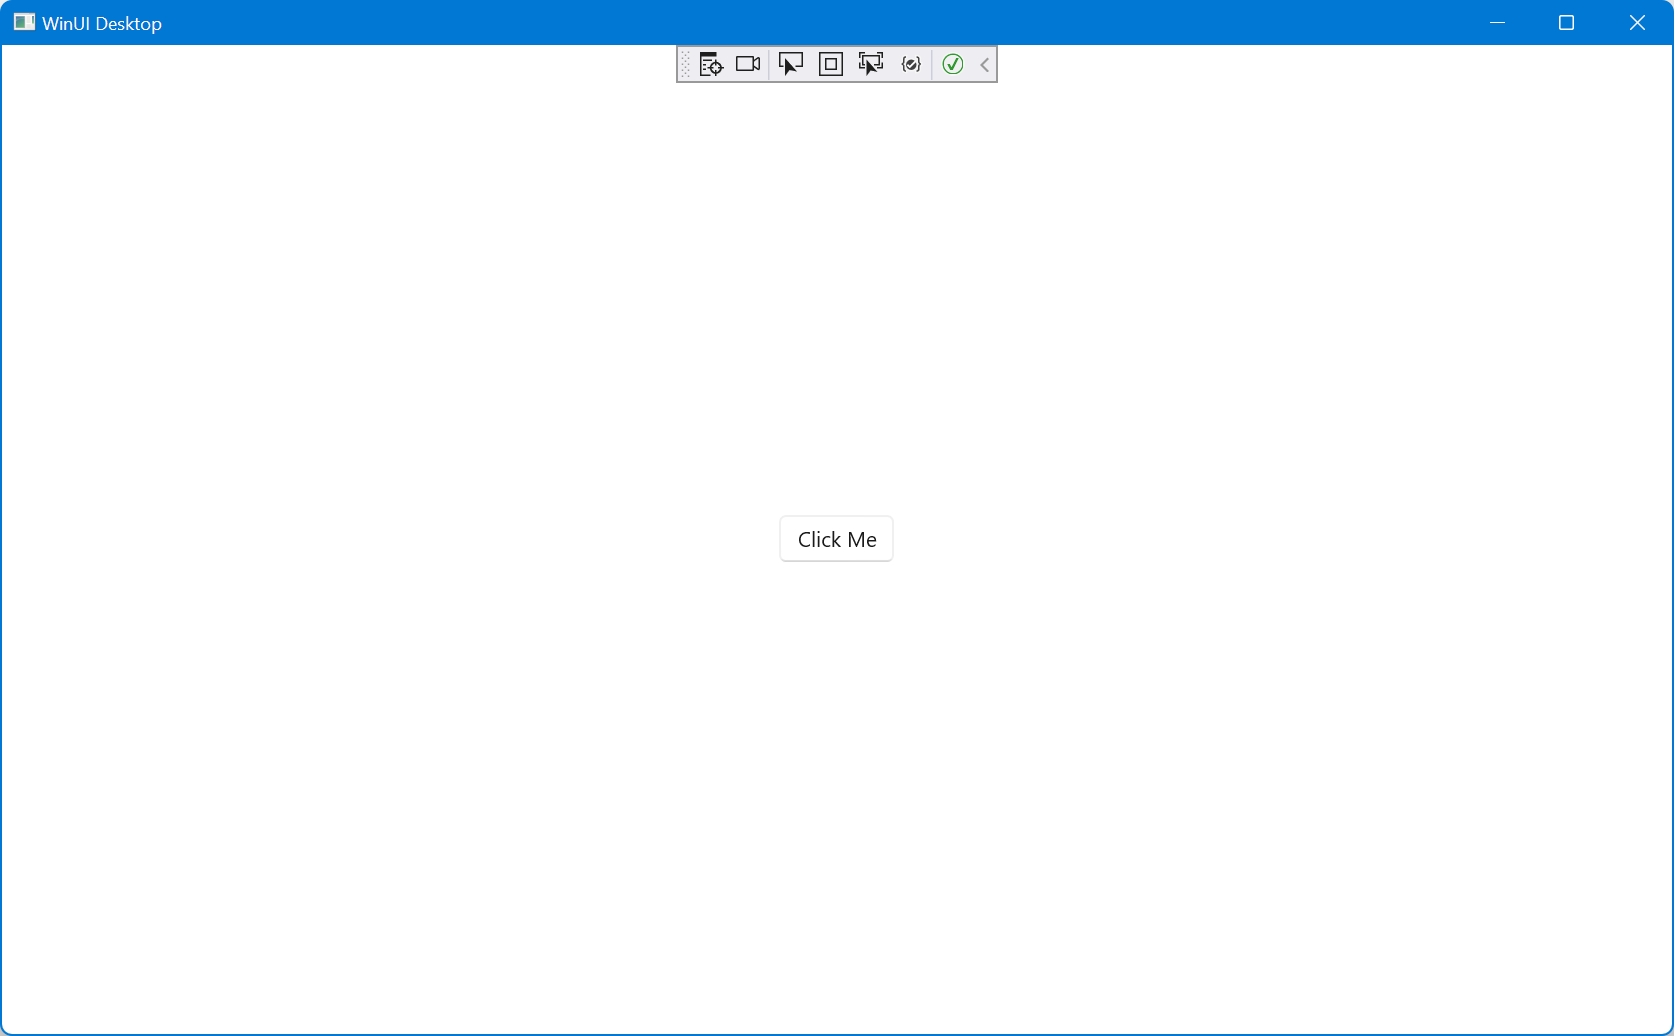
\includegraphics[width=\textwidth, height=\textheight, keepaspectratio]{Prototype-Button-Click-Me.png}

As expected, a window with a button shows up correctly. After clicking the button, the content in the button is changed to ``Clicked'' correctly.

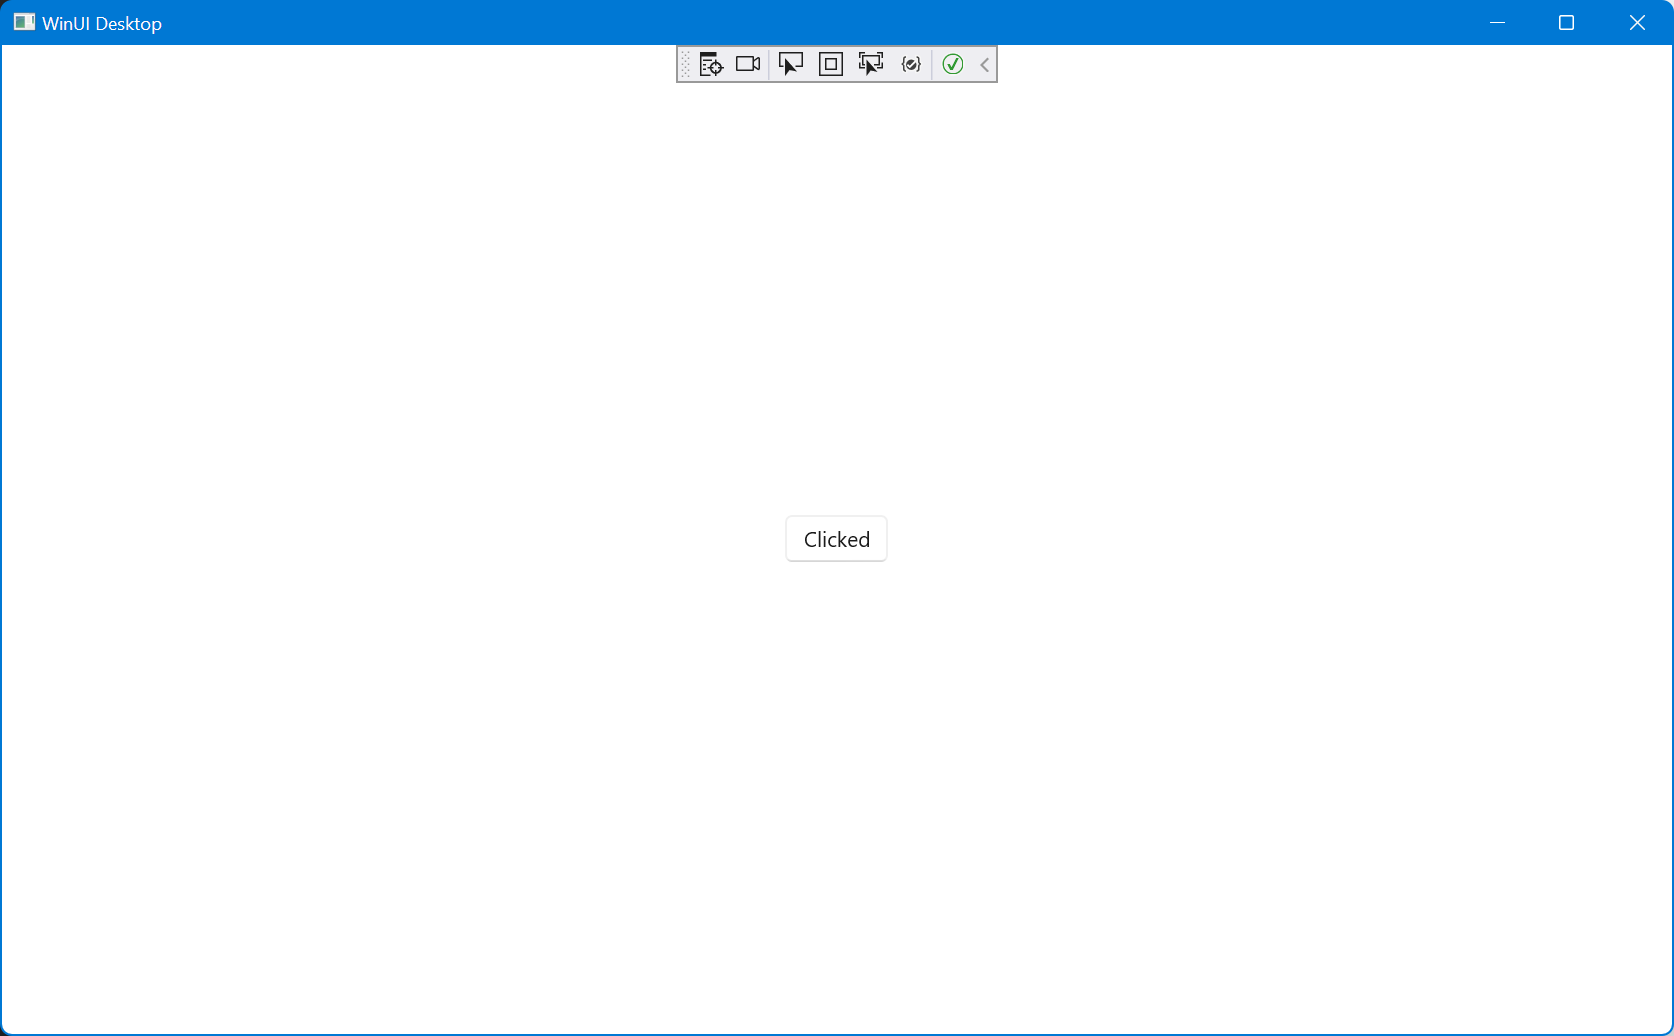
\includegraphics[width=\textwidth,height=\textheight,keepaspectratio]{Prototype-Button-Clicked.png}

\subsubsection{Testing and validation}

\begin{tabulary}{\linewidth}{|L|l|L|}
    \hline
    Test & Result & Remark \\
    \hline
    Does it compile & Pass & \\
    \hline
    Does it deploy & Pass & \\
    \hline
    Does it run & Pass & \\
    \hline
    Does the button work & Pass & \\
    \hline
\end{tabulary}

This is the simplest prototype, and its successful running means the development environment and the building tools are set up correctm, and I can start developing a more complex user interface.

\subsection{Create the NavigationView}

\subsubsection{Implementation}

First, I will implement the NavigationView as \hyperref[sec:NavigationViewDesign]{designed}. In the MainWindow.xaml file, I add the NavigationView control.

\begin{minted}{xml}
<NavigationView 
    x:Name="MainNavView"
    x:FieldModifier="public"
    IsBackButtonVisible="Collapsed"
    SelectionChanged="MainNavView_SelectionChanged">
</NavigationView>
\end{minted}

I assign a name \code{MainNavView} to the control so I can call it later in the code behind. I decide to hide the back button, which prevent the user to navigate the page in an unintended way. I also assign a \code{SelectionChanged} event handler to the control, which will be used to handle the navigation.

I then need to add different options to the navigation menu.

\begin{minted}{xml}
<NavigationView.MenuItems>
    <NavigationViewItem 
        x:Name="HomePageNavViewItem"
        Icon="Home"
        Content="Home"
        Tag="HomePage" />
    <NavigationViewItem
        x:Name="ProblemsPageNavViewItem"
        Icon="List"
        Content="Problems"
        Tag="ProblemsPage" />
    <NavigationViewItem
        x:Name="AssignmentsPageNavViewItem"
        Icon="Library"
        Content="Assignments"
        Tag="AssignmentsPage"/>
    <NavigationViewItem
        x:Name="PlaygroundPageNavViewItem"
        Icon="Edit"
        Content="Playground"
        Tag="PlaygroundPage"/>
</NavigationView.MenuItems>
\end{minted}

There are four options in the menu as designed. Each of which is assigned a name, icon, content and tag. The content and icon will be displayed to the user. The tag is used to identify the page that will be displayed when the option is clicked.

I add the account option to the footer.

\begin{minted}{xml}
<NavigationView.FooterMenuItems>
    <NavigationViewItem
        x:Name="AccountNavItem"
        Icon="Contact"
        Content="Account"
        Tag="AccountPage"/>
</NavigationView.FooterMenuItems>
\end{minted}

I add the content frame used to contain different pages.

\begin{minted}{xml}
<Frame
    x:Name="ContentFrame"
    Padding="0"
    Visibility="Visible"/>
\end{minted}

Now the layout of the NavigationView is finished. I need to add the code to initialize the control and handle the navigation.

When the main window is first initialized, the HomePage should be selected, and the title of the window should be set correctly. So I update the constructor of the main window to set the values.

\begin{minted}{csharp}
public MainWindow()
{
    InitializeComponent();
    Title = "Algorithm Dynamics";
    // Select HomePage when first loaded
    MainNavView.SelectedItem = MainNavView.MenuItems[0];
}
\end{minted}

Next, I need to handle the \code{SelectionChanged} event, this event gets triggered when the user clicks on a navigation item, and it will update the content frame to display the corresponding page.

\begin{minted}{csharp}
/// <summary>
/// Handle the SelectionChanged event of the MainNavView
/// Navigate to the corresponding page when the selection is changed
/// </summary>
/// <param name="sender"></param>
/// <param name="args"></param>
private void MainNavView_SelectionChanged(NavigationView sender, NavigationViewSelectionChangedEventArgs args)
{
    if (args.IsSettingsSelected)
    {
        // If the settings is selected, navigate to the settings page
        ContentFrame.Navigate(typeof(Pages.SettingsPage));
    }
    else
    {
        // Otherwise, get the selected item. If it is not null, get its Tag
        // Navigate to Algorithm_Dynamics.Pages.<Tag>
        NavigationViewItem selectedItem = args.SelectedItem as NavigationViewItem;
        if (selectedItem != null)
        {
            string tag = selectedItem.Tag as string;
            string pageName = "Algorithm_Dynamics.Pages." + tag;
            Type pageType = Type.GetType(pageName);
            ContentFrame.Navigate(pageType);
        }
    }
}
\end{minted}


Now, if I build and run the application, I should see the \code{NavigationView} works correctly. However, I get a runtime exception.

\begin{minted}{text}
System.NullReferenceException
  HResult=0x80004003
  Message=Object reference not set to an instance of an object.
  Source=WinRT.Runtime
  StackTrace:
   at ABI.System.Type.ToAbi(Type value)
   at ABI.System.Type.CreateMarshaler(Type value)
   at ABI.Microsoft.UI.Xaml.Controls.INavigate.global::Microsoft.UI.Xaml.Controls.INavigate.Navigate(Type sourcePageType)
   at Microsoft.UI.Xaml.Controls.Frame.Navigate(Type sourcePageType)
   at Algorithm_Dynamics.MainWindow.MainNavView_SelectionChanged(NavigationView sender, NavigationViewSelectionChangedEventArgs args) in C:\Algorithm-Dynamics\src\Algorithm Dynamics\MainWindow.xaml.cs:line 43
\end{minted}


It says object reference not set to an instance of an object when executing \code{ContentFrame.Navigate(pageType);}. This means the \code{pageType} does not exist. This is because I forget to create an actual HomePage, so it attempts to load a null object, failed, and throws the exception.  

I create all pages under the \code{Algorithm_Dynamics.Pages} namespace. For now, all of them will only contain a text block showing their name. Here is an example of the HomePage.

\begin{minted}{xml}
<Page
    x:Class="Algorithm_Dynamics.Pages.HomePage"
    xmlns="http://schemas.microsoft.com/winfx/2006/xaml/presentation"
    xmlns:x="http://schemas.microsoft.com/winfx/2006/xaml"
    xmlns:local="using:Algorithm_Dynamics.Pages"
    xmlns:d="http://schemas.microsoft.com/expression/blend/2008"
    xmlns:mc="http://schemas.openxmlformats.org/markup-compatibility/2006"
    mc:Ignorable="d"
    Background="{ThemeResource ApplicationPageBackgroundThemeBrush}">

    <Grid>
        <TextBlock Text="HomePage"/>
    </Grid>
</Page>
\end{minted}


\begin{minted}{csharp}
using Microsoft.UI.Xaml.Controls;

namespace Algorithm_Dynamics.Pages
{
    public sealed partial class HomePage : Page
    {
        public HomePage()
        {
            this.InitializeComponent();
        }
    }
}
\end{minted}

Now, the software build and run successfully. The HomePage is correctly selected when it is launched and the TextBlock HomePage shows up correctly means that the right page is loaded.

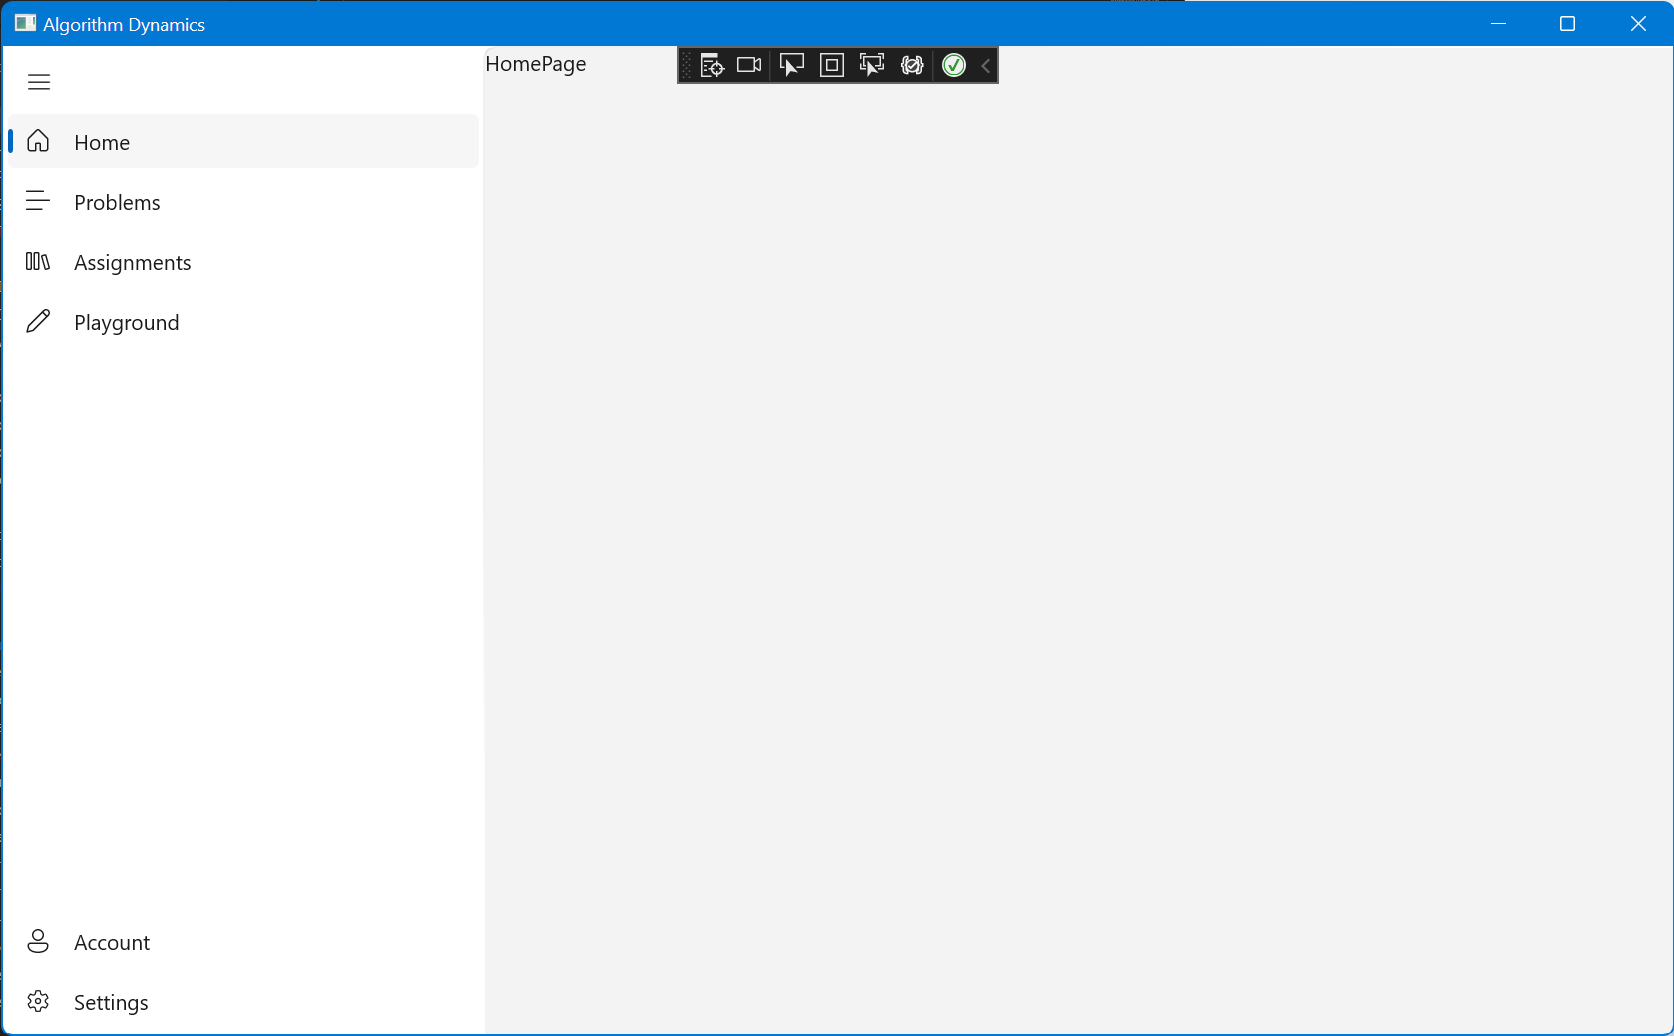
\includegraphics[width=\textwidth, height=\textheight, keepaspectratio]{HomePage-Draft-TextBlock}

When I click on other tabs on the NavigationView, the corresponding page is loaded correctly as well.

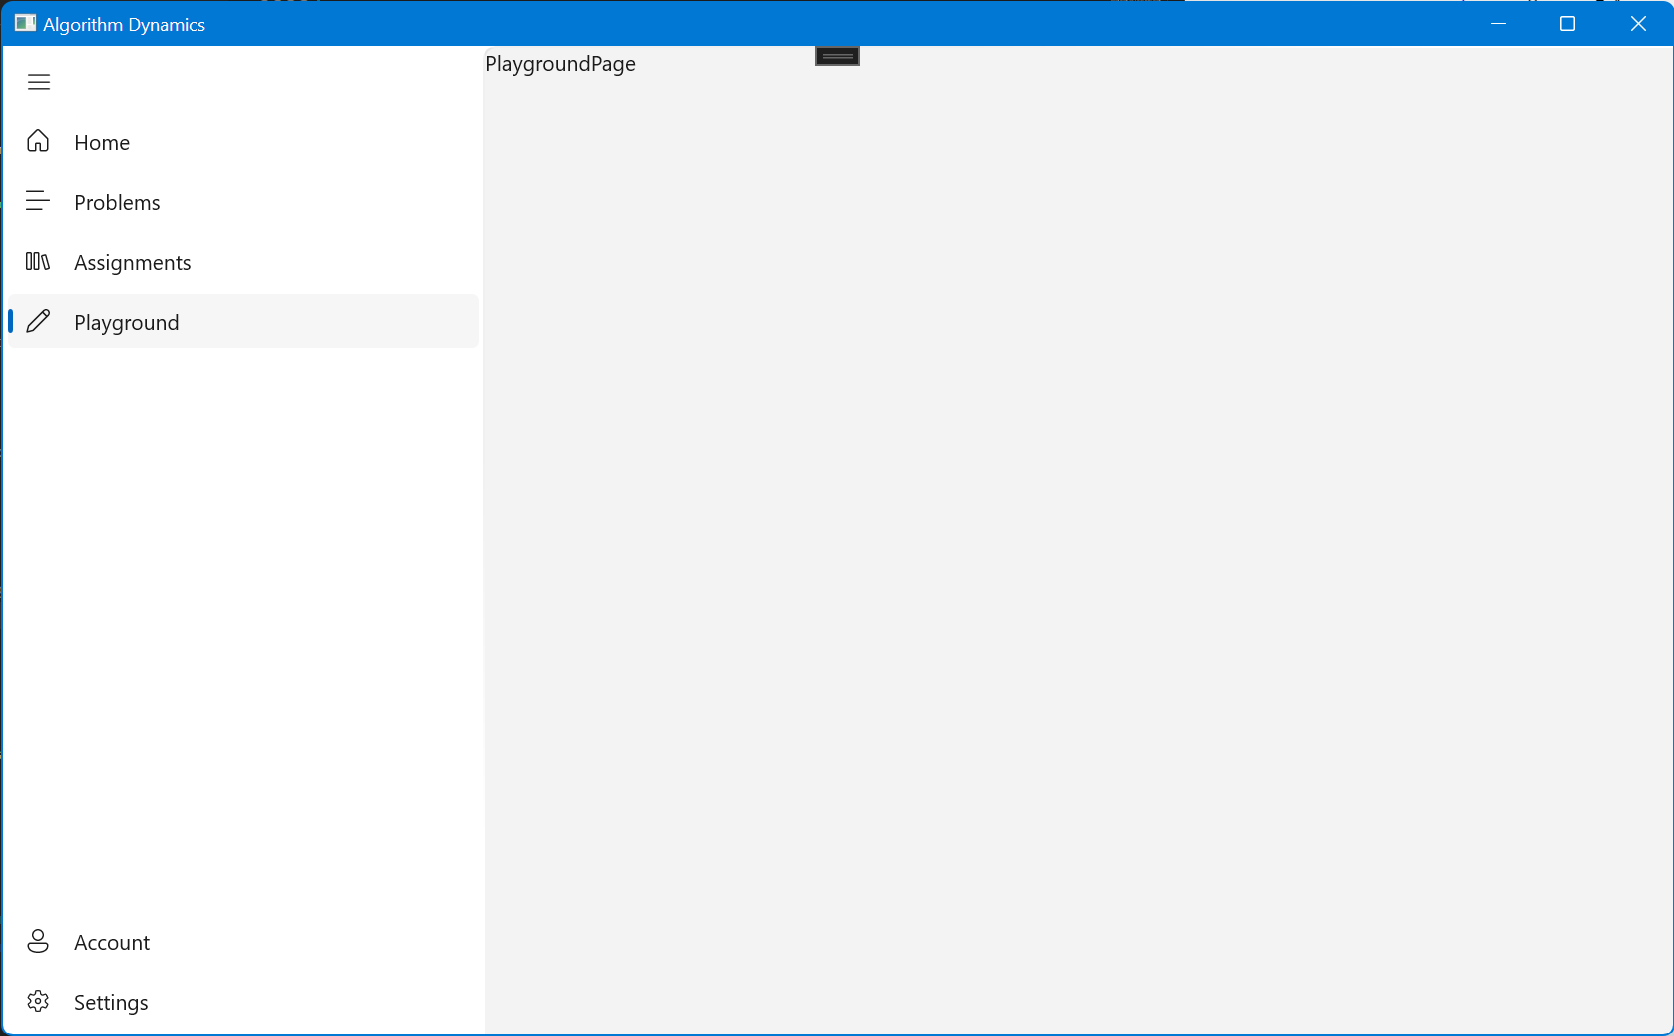
\includegraphics[width=\textwidth, height=\textheight, keepaspectratio]{PlaygroundPage-Draft-TextBlock}

\subsubsection{Testing and validation}

\begin{tabulary}{\linewidth}{|L|l|L|}
    \hline
    Test & Result & Remark \\
    \hline
    Does it load & Pass & \\
    \hline
    Does the button work & Pass & \\
    \hline
    Does it response to different screen size & Pass & \\
    \hline
\end{tabulary}

Now the NavigationView is built and tested. I will continue to build other components in the next section.

\subsection{Create the HomePage}

\subsubsection{Implementation}

The HomePage is made of three components, the background image, the quick access tools and the recommendations. They are wrapped by a scroller so they can be accessed on any size screen. I place a grid with two rows inside the \code{ScrollViewer}, the first row contains the background image, the second row contains the remaining tools. 

\begin{minted}{xml}
<Page
    x:Class="Algorithm_Dynamics.Pages.HomePage"
    xmlns="http://schemas.microsoft.com/winfx/2006/xaml/presentation"
    xmlns:x="http://schemas.microsoft.com/winfx/2006/xaml"
    xmlns:local="using:Algorithm_Dynamics.Pages"
    xmlns:models="using:Algorithm_Dynamics.Models"
    xmlns:controls="using:CommunityToolkit.WinUI.UI.Controls"
    xmlns:d="http://schemas.microsoft.com/expression/blend/2008"
    xmlns:mc="http://schemas.openxmlformats.org/markup-compatibility/2006"
    mc:Ignorable="d"
    Background="{ThemeResource ApplicationPageBackgroundThemeBrush}">
    <ScrollViewer>
        <Grid>
            <Grid.RowDefinitions>
                <RowDefinition Height="auto"/>
                <RowDefinition Height="auto"/>
            </Grid.RowDefinitions>
            <Grid Grid.Row="0">
                <!-- Background Image -->
            </Grid>
            <Grid 
                Margin="24"
                Grid.Row="1">
                <!-- Quick Access tools and Recommendations -->
            </Grid>
        </Grid>
    </ScrollViewer>
</Page>
\end{minted}

Inside the background image grid, I place a \code{Image} control with the source of the background image. It is stretched to fill the entire grid so \code{Strecth} is set to \code{UniformToFill}.

\begin{minted}{xml}
<Image 
    Source="/Assets/HomePageBackgroundImage.jpg" 
    Height="256"
    Stretch="UniformToFill"/>
<TextBlock 
    Text="{x:Bind WelcomeMessage, Mode=OneTime, FallbackValue='Welcome User'}"
    HorizontalAlignment="Right"
    VerticalAlignment="Bottom"
    Margin="8"
    Foreground="White"
    Style="{ThemeResource TitleTextBlockStyle}"/>
\end{minted}

The \code{TextBlock} is used to display a greeting message. It is placed on the bottom right. Because its content needs to be adjusted by the current time and the current user, it is binded to the a variable \code{WelcomeMessage} so I can change its value programmatically.

\begin{minted}{csharp}
namespace Algorithm_Dynamics.Pages
{
    public sealed partial class HomePage : Page
    {
        /// <summary>
        /// The WelcomeMessage is displayed to the user on the HomePage
        /// </summary>
        public string WelcomeMessage { get; set; }
        public HomePage()
        {
            InitializeComponent();
        }
    }
}
\end{minted}

The welcome message is adjusted by different time in the day. It should also display the user name, but since the settings module is not implemented yet, I use a placeholder for the user name.

\begin{minted}{csharp}
/// <summary>
/// Set the WelcomeMessage based on the current time.
/// Morning: 00:00-12:00
/// Afternoon: 12:00-17:00
/// Evening 17:00-0:00
/// TODO Add the username after it is implemented
/// </summary>
private void SetWelcomeMessage()
{
    TimeSpan now = DateTime.Now.TimeOfDay;
    if (now >= new TimeSpan(00, 00, 00) && now < new TimeSpan(12, 00, 00))
    {
        WelcomeMessage = "Good morning, user!";
    }
    else if (now >= new TimeSpan(12, 00, 00) && now < new TimeSpan(17, 00, 00))
    {
        WelcomeMessage = "Good afternoon, user!";
    }
    else if (now >= new TimeSpan(17, 00, 00) && now <= new TimeSpan(23, 59, 59))
    {
        WelcomeMessage = "Good evening, user!";
    }
}
\end{minted}

Now I just need to set the welcome message in the constructor. Notice that it needs to be called before all components are initialized, so the text block can bind to the updated value.

\begin{minted}{csharp}
public HomePage()
{
    SetWelcomeMessage();
    InitializeComponent();
}
\end{minted}

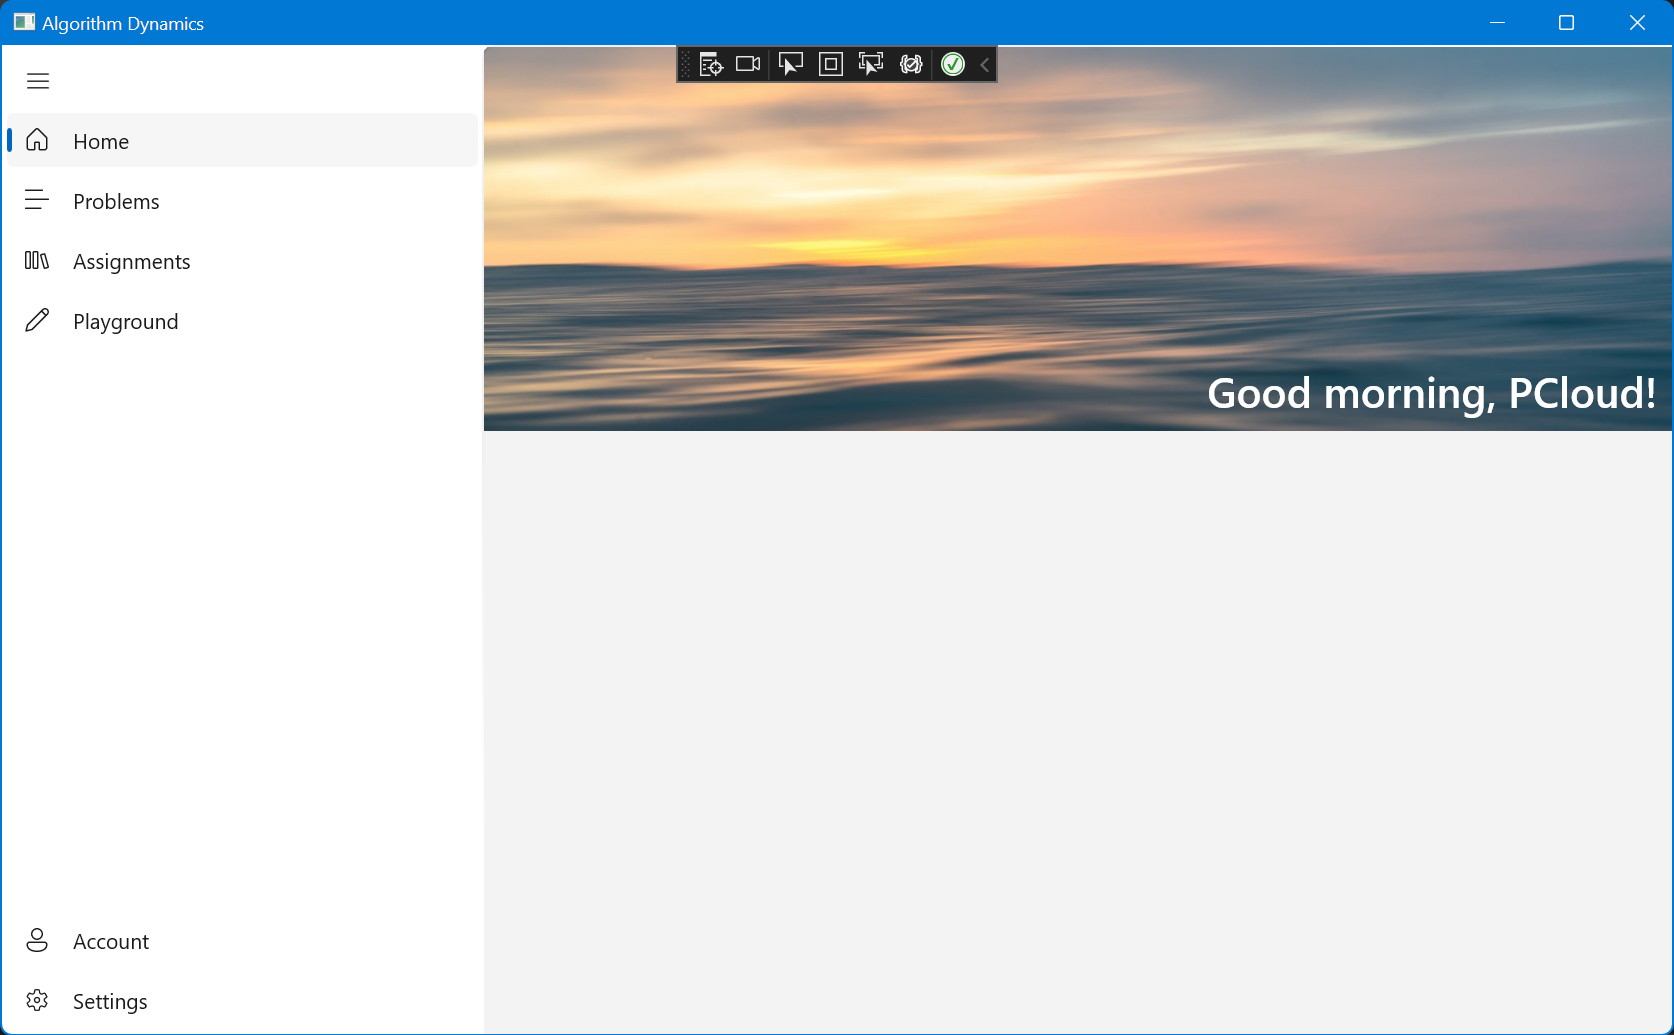
\includegraphics[width=\textwidth, height=\textheight, keepaspectratio]{HomePage-Image}

The image and the greeting message show up correctly, and because I am writing this in the morning, the correct greeting message is displayed.

For the quick access toolbar, I choose to use the \code{AdaptiveGridView} control for its \code{OneRowMode} function, which allows the toolbar to scroll horizontally on small screens. The controls in the quick access toolbar should be loaded dynamically, so they can be changed easily in the future. So I create a \code{QuickAccessItem} helper class. Each object will contain a name, an icon and an action. The name and the icon will be displayed to the user, and the action will be invoked when the user clicks on the control.

\begin{minted}{csharp}
using Microsoft.UI.Xaml.Controls;
using System;

namespace Algorithm_Dynamics.Models
{
    public class QuickAccessItem
    {
        public string Name { get; set; }
        public Symbol Icon { get; set; }
        public Action<MainWindow> Action { get; set; }
        public QuickAccessItem(string name, Symbol icon, Action<MainWindow> action)
        {
            Name = name;
            Icon = icon;
            Action = action;
        }
    }
}
\end{minted}

Then I create a \code{ObserableCollection} of \code{QAItems} that binds to the grid.

\begin{minted}{csharp}
public ObservableCollection<QuickAccessItem> QAItems { get; } = new ObservableCollection<QuickAccessItem>();
\end{minted}

\begin{minted}{xml}
<TextBlock 
    Text="Quick Access"
    Grid.Row="0"
    Style="{ThemeResource SubtitleTextBlockStyle}"/>
<controls:AdaptiveGridView 
    Grid.Row="1"
    Margin="4"
    ItemsSource="{x:Bind QAItems}"
    StretchContentForSingleRow="True"
    OneRowModeEnabled="True"
    ItemHeight="160"
    DesiredWidth="160"
    SelectionMode="None"
    IsItemClickEnabled="True">
    <GridView.ItemTemplate>
        <DataTemplate x:DataType="models:QuickAccessItem">
            <StackPanel 
                VerticalAlignment="Center"
                HorizontalAlignment="Center"
                Orientation="Vertical">
                <SymbolIcon 
                    x:Name="ItemIcon"
                    Symbol="{x:Bind Icon}"/>
                <TextBlock Text="{x:Bind Name}" />
            </StackPanel>
        </DataTemplate>
    </GridView.ItemTemplate>
</controls:AdaptiveGridView>
\end{minted}

I need to add the items to the collection when the HomePage is loaded. I create a procedure \code{InitializeQAItems}. Because I have passed the MainWindow object to the function, the MainNavView can be called inside. Because the CodingPage and the import/export logic is not completed yet, the Random Problem and Import function will be implemented later.

\begin{minted}{csharp}
public HomePage()
{
    SetWelcomeMessage();
    InitializeQAItems();
    InitializeComponent();
}
private void InitializeQAItems()
{
    QAItems.Clear();
    QAItems.Add(new QuickAccessItem("Random Problem", Symbol.Shuffle, (m_window) =>
    {
        m_window.MainNavView.SelectedItem = null;
        // TODO Navigate the ContentFrame to the Coding page manually
        throw new NotImplementedException("[Blocking]: The CodingPage has not been implemented yet.");
    }));
    QAItems.Add(new QuickAccessItem("Playground", Symbol.Edit, (m_window) =>
        m_window.MainNavView.SelectedItem = m_window.MainNavView.MenuItems[1]));
    QAItems.Add(new QuickAccessItem("Assignments", Symbol.Library, (m_window) =>
        m_window.MainNavView.SelectedItem = m_window.MainNavView.MenuItems[2]));
    QAItems.Add(new QuickAccessItem("Problems", Symbol.List, (m_window) =>
        m_window.MainNavView.SelectedItem = m_window.MainNavView.MenuItems[3]));
    QAItems.Add(new QuickAccessItem("Settings", Symbol.Setting, (m_window) =>
        m_window.MainNavView.SelectedItem = m_window.MainNavView.SettingsItem));
    QAItems.Add(new QuickAccessItem("Account", Symbol.Contact, (m_window) =>
        m_window.MainNavView.SelectedItem = m_window.MainNavView.FooterMenuItems[0]));
    QAItems.Add(new QuickAccessItem("Import", Symbol.Import, (m_window) =>
    {
        m_window.MainNavView.SelectedItem = null;
        // TODO Handle the import logic
        throw new NotImplementedException("[Blocking]: The import logic has not been implemented yet.");
    }));
}
\end{minted}

I need to handle the click event of the quick access toolbar. I create a procedure \code{QAGridView_ItemClick}, which will invoke the action of the item.

\begin{minted}{csharp}
/// <summary>
/// Handle the QAGridView click event. The Action will be invoked.
/// </summary>
/// <param name="sender"></param>
/// <param name="e"></param>
private void QAGridView_ItemClick(object sender, ItemClickEventArgs e)
{
    MainWindow m_window = (MainWindow)((App)Application.Current).m_window;
    if (e.ClickedItem is QuickAccessItem item)
    {
        item.Action(m_window);
    }
}
\end{minted}

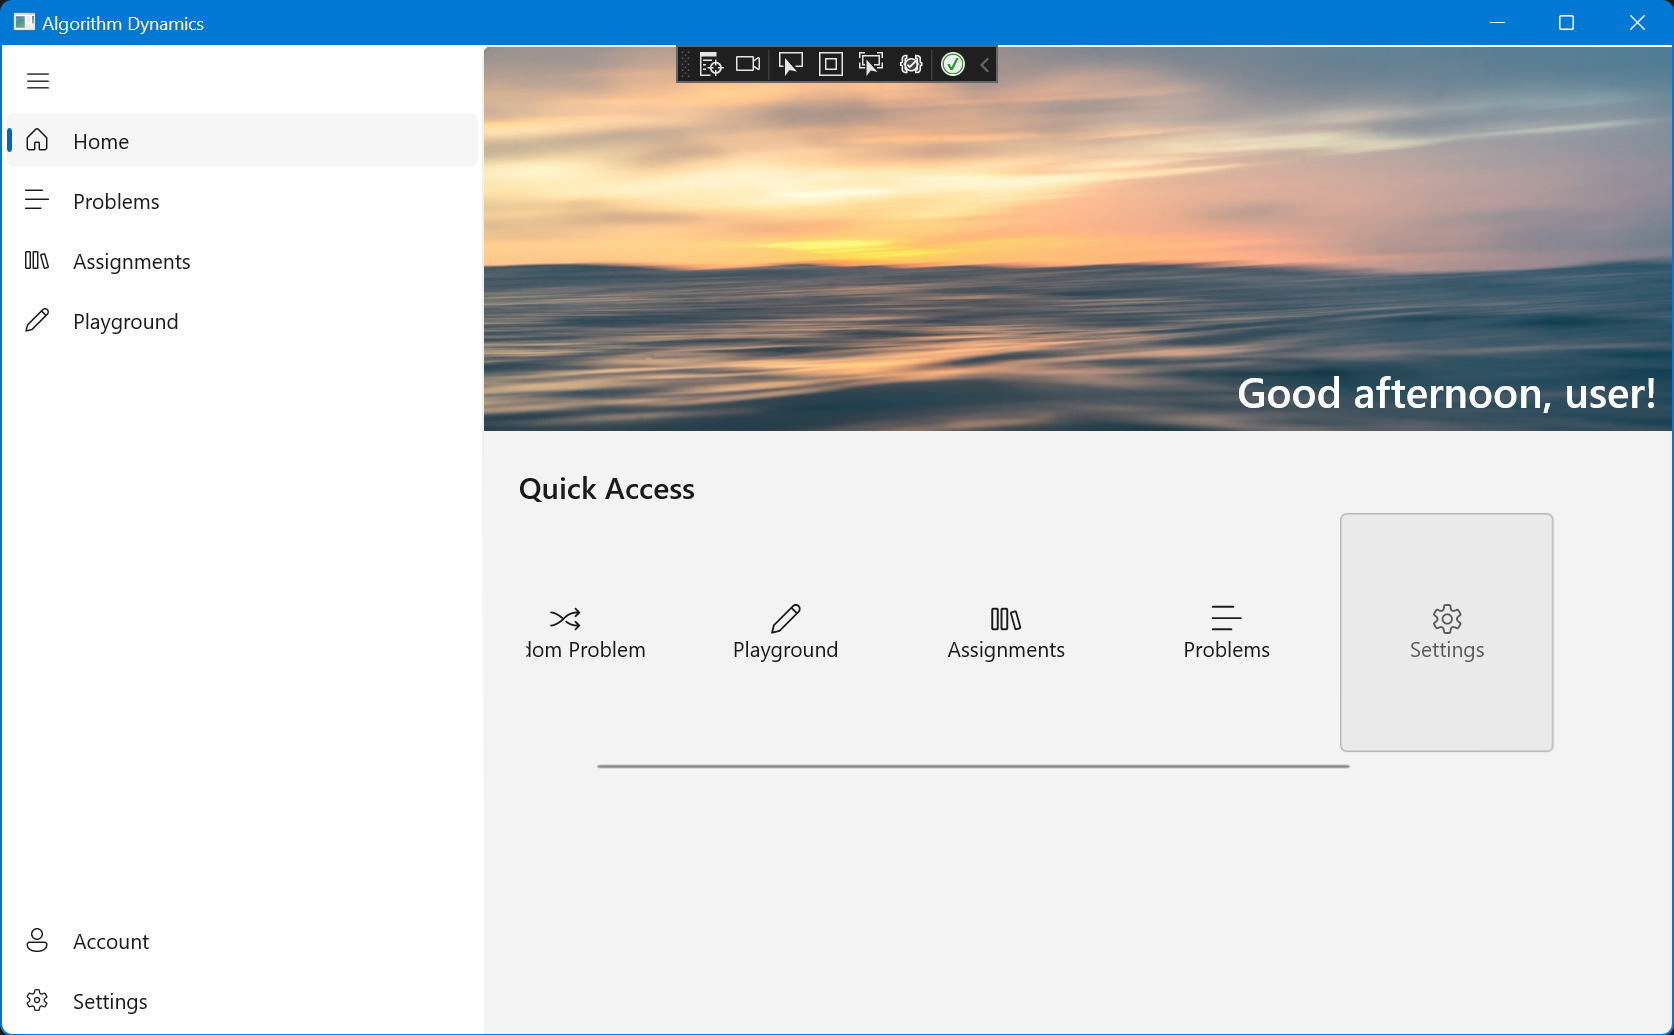
\includegraphics[width=\textwidth, height=\textheight, keepaspectratio]{HomePage-QuickAccessToolbar.png}

Now, when I build and run the application, the quick access toolbar shows up correctly and scroll horizontally as expected. When I click the different buttons, it navigates to the corresponding page correctly. When I click the Random Problem button, the software panic and a NotImplementedException is thrown with the correct error message.

\begin{minted}{text}
System.NotImplementedException
  HResult=0x80004001
  Message=[Blocking]: The CodingPage has not been implemented yet.
  Source=Algorithm Dynamics
  StackTrace:
   at Algorithm_Dynamics.Pages.HomePage.<>c.<InitializeQAItems>b__13_0(MainWindow m_window) in C:\Algorithm-Dynamics\src\Algorithm Dynamics\Pages\HomePage.xaml.cs:line 70
   at Algorithm_Dynamics.Pages.HomePage.QAGridView_ItemClick(Object sender, ItemClickEventArgs e) in C:\Algorithm-Dynamics\src\Algorithm Dynamics\Pages\HomePage.xaml.cs:line 59
   at WinRT._EventSource_global__Microsoft_UI_Xaml_Controls_ItemClickEventHandler.EventState.<GetEventInvoke>b__1_0(Object sender, ItemClickEventArgs e)
   at ABI.Microsoft.UI.Xaml.Controls.ItemClickEventHandler.<>c__DisplayClass10_0.<Do_Abi_Invoke>b__0(ItemClickEventHandler invoke)
   at ABI.Microsoft.UI.Xaml.Controls.ItemClickEventHandler.Do_Abi_Invoke(IntPtr thisPtr, IntPtr sender, IntPtr e)
\end{minted}

The recommendation control is similar. I create the \code{RecommendItem} class and add the items to the collection.

\begin{minted}{csharp}
namespace Algorithm_Dynamics.Models
{
    public class RecommendItem
    {
        public string Title { get; set; }
        public string Description { get; set; }
        public RecommendItem(string title, string description)
        {
            Title = title;
            Description = description;
        }
    }
}
\end{minted}

\begin{minted}{csharp}
public ObservableCollection<RecommendItem> RecItems { get; } = new ObservableCollection<RecommendItem>();
\end{minted}

Then bind the AdaptiveGridView to the collection.

\begin{minted}{csharp}
<TextBlock 
    Text="Recommended"
    Grid.Row="2"
    Style="{ThemeResource SubtitleTextBlockStyle}"/>
<controls:AdaptiveGridView
    x:Name="RecGridView"
    Grid.Row="3"
    Margin="4"
    ItemsSource="{x:Bind RecItems}"
    StretchContentForSingleRow="False"
    OneRowModeEnabled="False"
    ItemHeight="80"
    DesiredWidth="320"
    SelectionMode="None"
    IsItemClickEnabled="True"
    ItemClick="RecGridView_ItemClick">
    <GridView.ItemTemplate>
        <DataTemplate x:DataType="models:RecommendItem">
            <Grid HorizontalAlignment="Stretch">
                <StackPanel 
                    VerticalAlignment="Center"
                    HorizontalAlignment="Left"
                    Orientation="Vertical"
                    Margin="8">
                    <TextBlock Text="{x:Bind Title}"
                                Style="{ThemeResource BodyStrongTextBlockStyle}"/>
                    <TextBlock Text="{x:Bind Description}"/>
                </StackPanel>
            </Grid>
        </DataTemplate>
    </GridView.ItemTemplate>
</controls:AdaptiveGridView>
\end{minted}

For now, because the database and the data structure are not ready, I just add some dummy data to the collection. The recommendation logic will be added later.

\begin{minted}{csharp}
public HomePage()
{
    SetWelcomeMessage();
    InitializeQAItems();
    InitializeRecItems();
    InitializeComponent();
}
/// <summary>
/// TODO Generate Recommendation from database.
/// </summary>
private void InitializeRecItems()
{
    RecItems.Clear();
    RecItems.Add(new RecommendItem("Problem 1", "Easy | Data structure"));
    RecItems.Add(new RecommendItem("Problem 2", "Medium | Sorting"));
    RecItems.Add(new RecommendItem("Problem 3", "Hard | Graph"));
    RecItems.Add(new RecommendItem("Problem 4", "Easy | Data structure"));
    RecItems.Add(new RecommendItem("Assignment 1", "Due in 2 days"));
    RecItems.Add(new RecommendItem("Assignment 2", "Due in 3 days"));
    RecItems.Add(new RecommendItem("Assignment 3", "Due in 4 days"));
    RecItems.Add(new RecommendItem("Assignment 4", "Due in 5 days"));
}
\end{minted}

I need to handle the click event as well. And because neither the AssignmentsPage nor the CodingPage is ready, it will throw an NotImplementedException too.

\begin{minted}{csharp}
/// <summary>
/// Handle the RecGridView click event.
/// Navigate to the corresponding Problem or Assignment
/// </summary>
/// <param name="sender"></param>
/// <param name="e"></param>
private void RecGridView_ItemClick(object sender, ItemClickEventArgs e)
{
    // TODO Handle the navigation.
    throw new NotImplementedException("[Blocking]: The CodingPage or the AssignmentsPage has not been implemented yet.");
}
\end{minted}

Now, the HomePage is implemented. I run the application and test it.

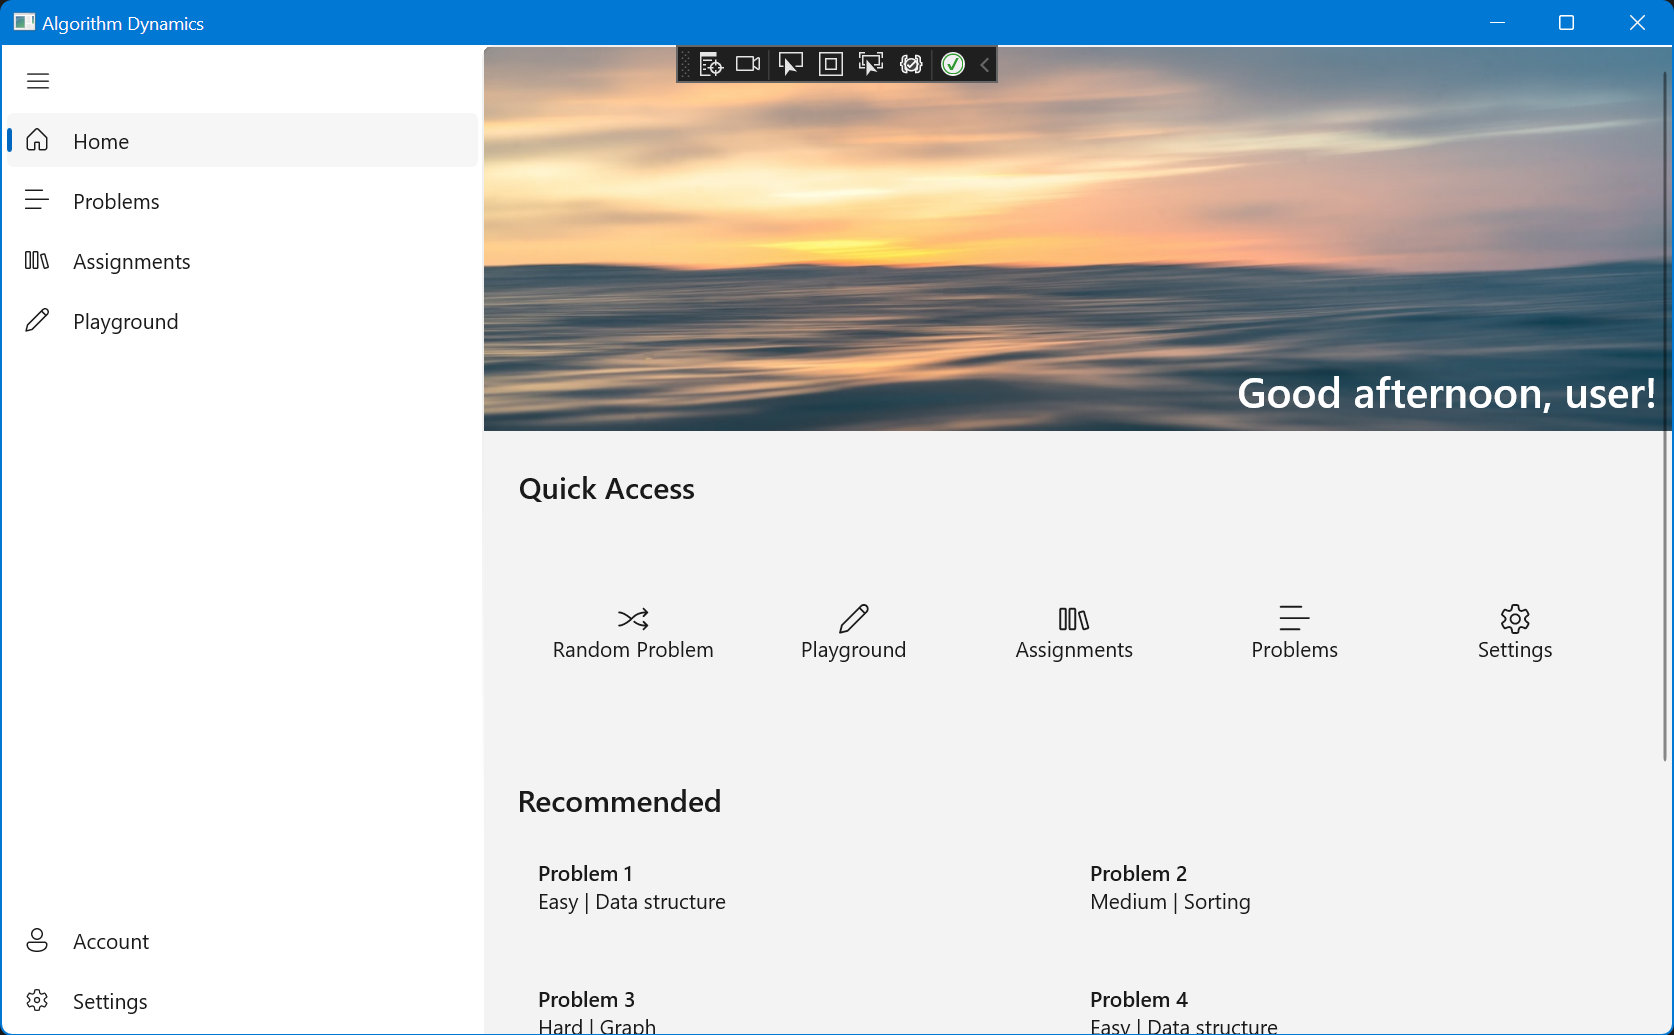
\includegraphics[width=\textwidth, height=\textheight, keepaspectratio]{HomePage-Finished}

All components show up correctly. The image is loaded and the greeting message is correct. The Quick Access Toolbar navigates correctly. When I click the recommended item, the correct exception is thrown.

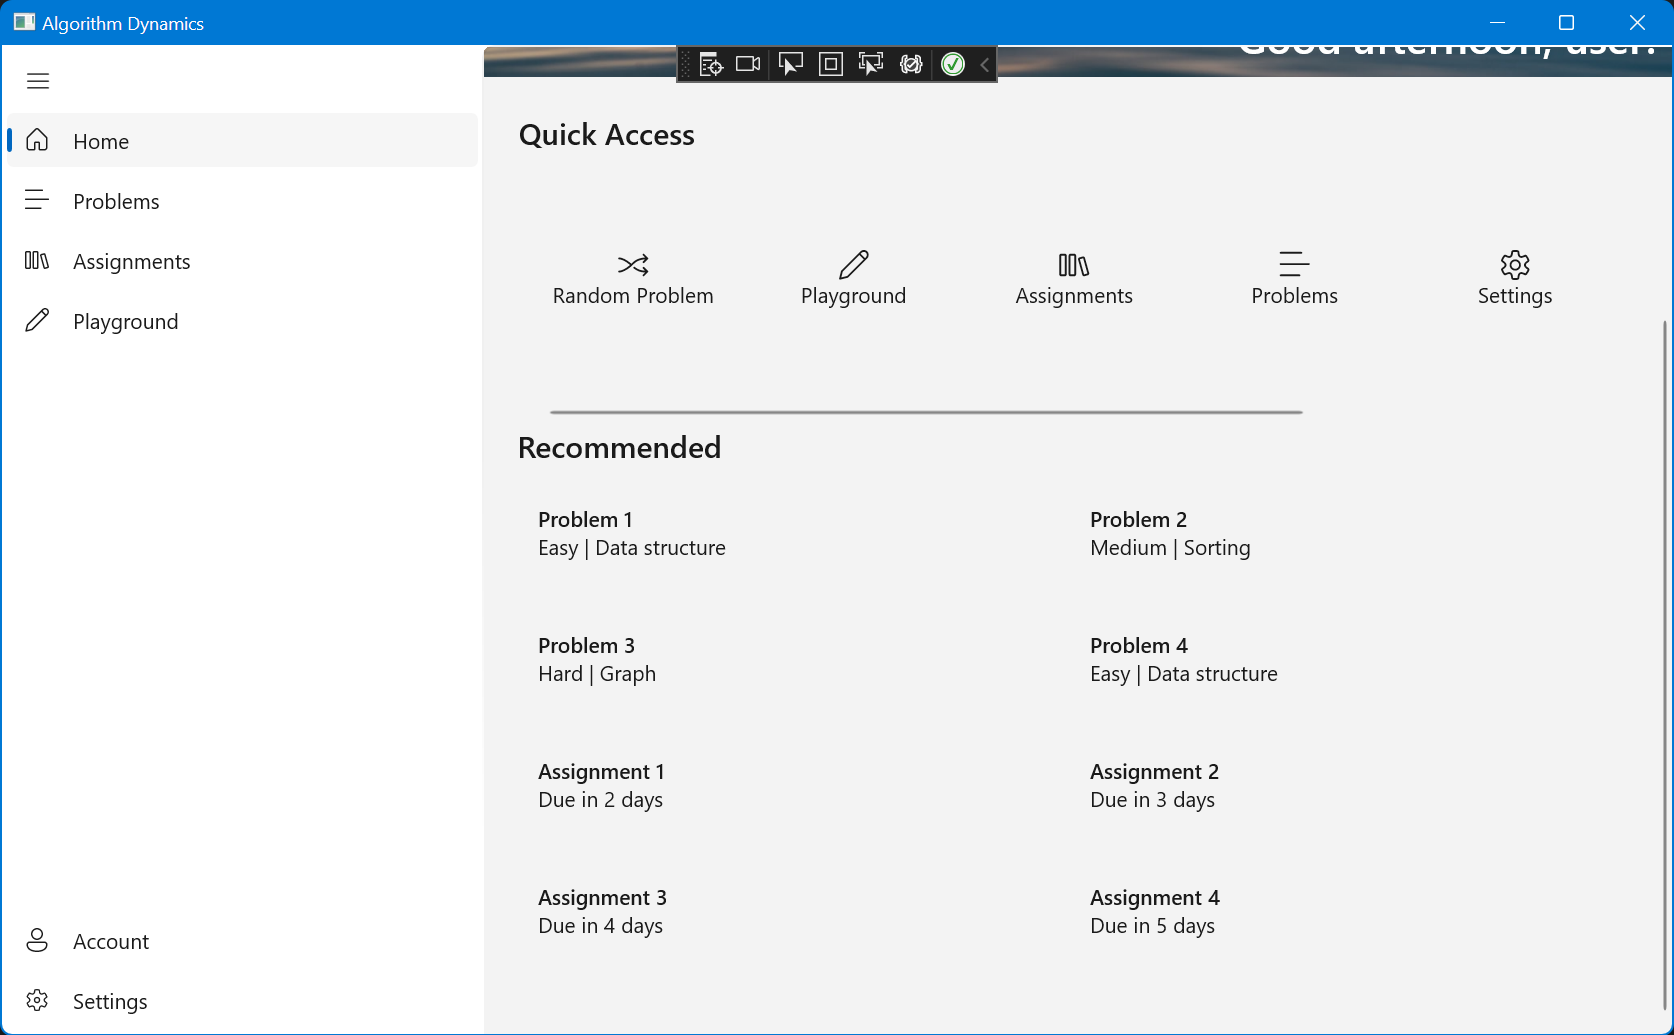
\includegraphics[width=\textwidth, height=\textheight, keepaspectratio]{HomePage-Finished-Scroll}

The scroller is working as well, so I can scroll down on a small window to see the recommendation items.

\subsubsection{Testing and validation}

\begin{tabulary}{\linewidth}{|L|l|L|}
    \hline
    Test & Result & Remark \\
    \hline
    Does it load & Pass & \\
    \hline
    Does the background image show up correctly & Pass & \\
    \hline
    Does the greeting message show up correctly & Pass & \\
    \hline
    Does the Quick Access Toolbar show up correctly & Pass & \\
    \hline
    Does the Quick Access Toolbar work correctly & Failed & The Random Problems and data import function is not implemented and will be implemented in the future. This test case will be reviewed then. \\
    \hline
    Does the Recommendation show up correctly & Pass &  \\
    \hline
    Does the Recommendation work correctly & Failed & The database and the data structure will be implemented in the future. This test case will be reviewed then. \\
    \hline
    Is the page responsive & Pass & \\
    \hline
\end{tabulary}

\subsection{Create the ProblemsPage}

\subsubsection{Implementation}

I move on to design the ProblemsPage. It contains two parts, the toolbar at the top and the problem list below. I will use a grid containing two rows to hold these two components.

\begin{minted}{xml}
<Page
    x:Class="Algorithm_Dynamics.Pages.ProblemsPage"
    xmlns="http://schemas.microsoft.com/winfx/2006/xaml/presentation"
    xmlns:x="http://schemas.microsoft.com/winfx/2006/xaml"
    xmlns:local="using:Algorithm_Dynamics.Pages"
    xmlns:d="http://schemas.microsoft.com/expression/blend/2008"
    xmlns:mc="http://schemas.openxmlformats.org/markup-compatibility/2006"
    mc:Ignorable="d"
    Background="{ThemeResource ApplicationPageBackgroundThemeBrush}">
    <Grid>
        <Grid.RowDefinitions>
            <RowDefinition Height="auto"/>
            <RowDefinition Height="*"/>
        </Grid.RowDefinitions>
        <Grid
            Grid.Row="0"
            HorizontalAlignment="Stretch">
            <!-- Toolbar -->
        </Grid>
        <Grid
            Grid.Row="1"
            HorizontalAlignment="Stretch">
            <!-- Problem List -->
        </Grid>
    </Grid>
</Page>
\end{minted}

For the toolbar, I use a grid with 6 columns to hold the search box and the ComboBoxes.

\begin{minted}{xml}
<Grid.ColumnDefinitions>
    <ColumnDefinition Width="2*"/>
    <ColumnDefinition Width="*"/>
    <ColumnDefinition Width="*"/>
    <ColumnDefinition Width="*"/>
    <ColumnDefinition Width="*"/>
    <ColumnDefinition Width="*"/>
</Grid.ColumnDefinitions>
<AutoSuggestBox 
    Grid.Column="0"
    Margin="4"
    PlaceholderText="Search..."
    x:Name="ProblemsSearchBox"
    HorizontalAlignment="Stretch"/>
<ComboBox 
    PlaceholderText="Difficulty"
    Grid.Column="1"
    Margin="4"
    ItemsSource="{x:Bind Difficulties}"
    HorizontalAlignment="Stretch"/>
<ComboBox 
    PlaceholderText="Status"
    Grid.Column="2"
    Margin="4"
    ItemsSource="{x:Bind Statuses}"
    HorizontalAlignment="Stretch"/>
<ComboBox 
    PlaceholderText="Tag"
    Grid.Column="3"
    Margin="4"
    ItemsSource="{x:Bind Tags}"
    HorizontalAlignment="Stretch"/>
<ComboBox 
    PlaceholderText="List"
    x:Name="ListComboBox"
    Grid.Column="4"
    Margin="4"
    ItemsSource="{x:Bind Lists}"
    HorizontalAlignment="Stretch"/>
<DropDownButton 
    Content="Add"
    Grid.Column="6"
    Margin="4"
    HorizontalAlignment="Stretch">
    <DropDownButton.Flyout>
        <MenuFlyout Placement="Bottom">
            <MenuFlyoutItem Text="New Problem"/>
            <MenuFlyoutItem Text="New Problem List"/>
            <MenuFlyoutItem Text="Import"/>
        </MenuFlyout>
    </DropDownButton.Flyout>
</DropDownButton>
\end{minted}

The ItemsSource of the ComboBox is binded to the corresponding variable, which allows me to set their value programmatically. Because the database is not implemented yet, I will use some dummy data to test the UI.

\begin{minted}{csharp}
using Microsoft.UI.Xaml.Controls;
using System.Collections.ObjectModel;

namespace Algorithm_Dynamics.Pages
{
    public sealed partial class ProblemsPage : Page
    {
        public ProblemsPage()
        {
            this.InitializeComponent();
        }
        private readonly ObservableCollection<string> Difficulties = new() { "Easy", "Medium", "Hard" };
        private readonly ObservableCollection<string> Statuses = new() { "Todo", "Attempted", "Done" };
        public ObservableCollection<string> Lists = new() { "List 1", "List 2", "List 3" };
        public ObservableCollection<string> Tags = new() { "Tag 1", "Tag 2", "Tag 3"};
    }
}
\end{minted}

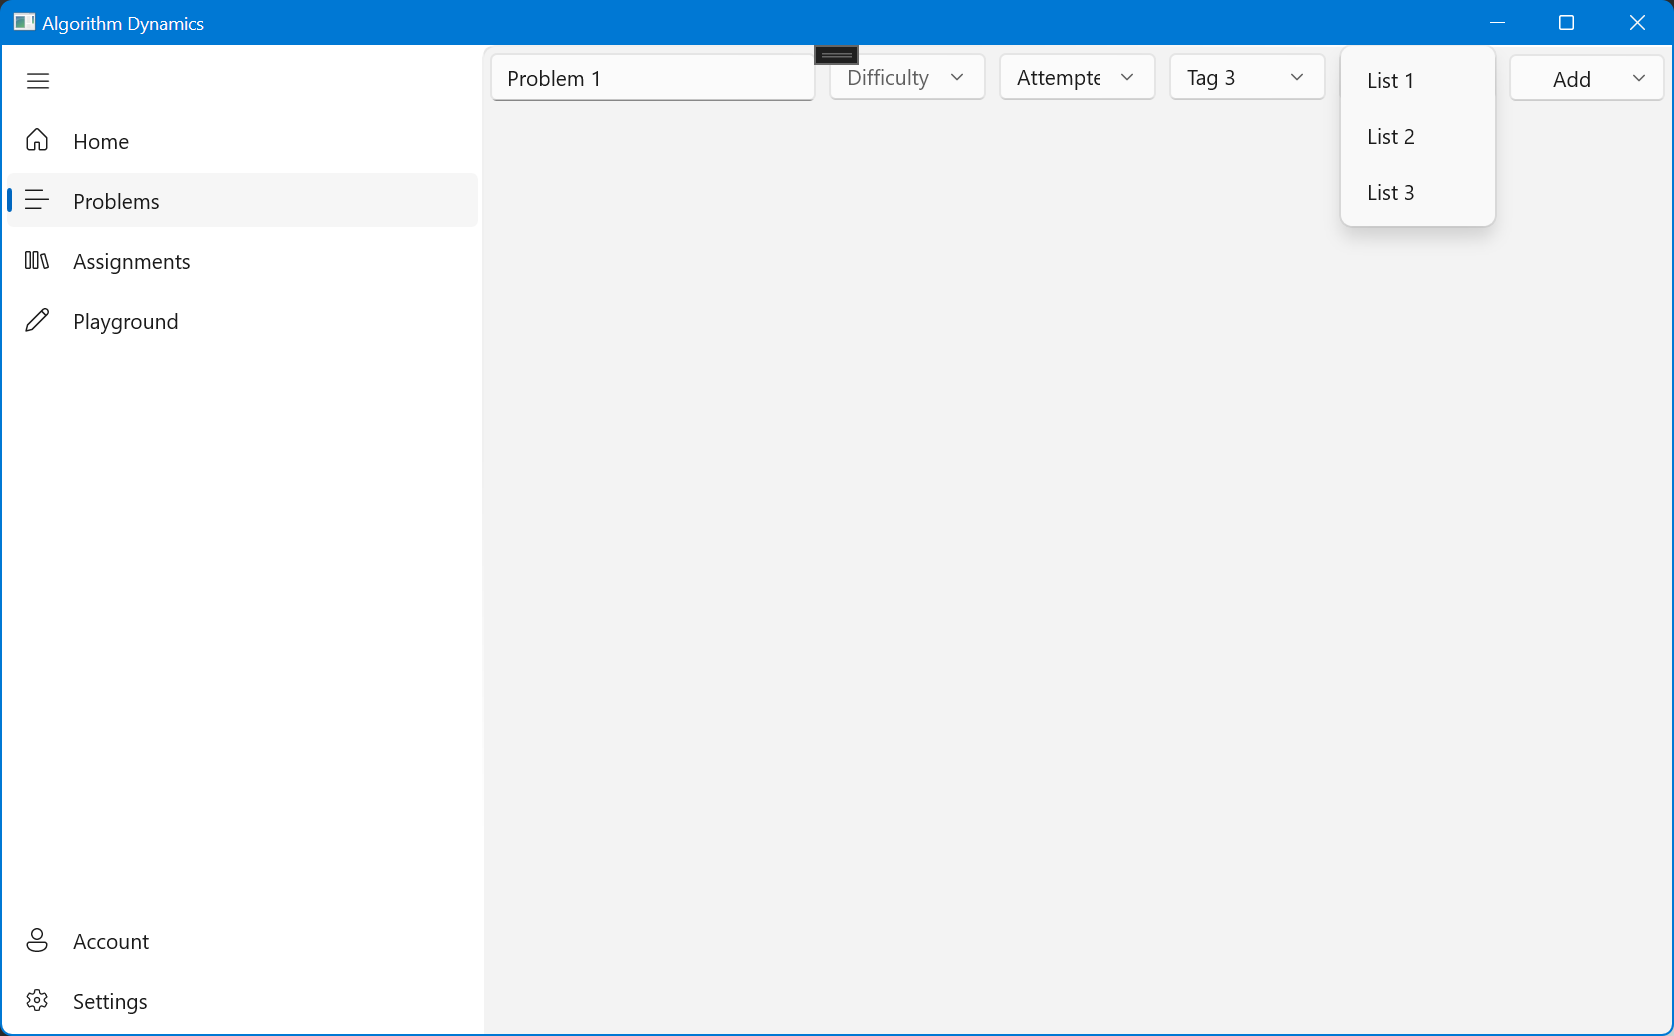
\includegraphics[width=\textwidth, height=\textheight, keepaspectratio]{ProblemsPage-Toolbar}

The toolbar shows up with all data loaded correctly. I can select an item correctly, but I cannot clear the selection. I need to empty the ComboBox when the user right clicks it. For the list ComboBox, I also need to allow the user to edit and delete an existing list, so when the user right click the list ComboBox, a menu flyout needs to show up with all options. I create a \code{ClearComboBox} procedure to handle the right click event.

\begin{minted}{csharp}
/// <summary>
/// Clear the <see cref="ComboBox"/>
/// </summary>
/// <param name="sender"></param>
/// <param name="e"></param>
private void ClearComboBox(object sender, RightTappedRoutedEventArgs e)
{
    ComboBox comboBox = (ComboBox)sender;
    comboBox.SelectedIndex = -1;
}
\end{minted}

And then bind the right clicked event to the procedure.

\begin{minted}{xml}
<ComboBox
    x:Name="DifficultyComboBox"
    RightTapped="ClearComboBox"/>
<ComboBox
    x:Name="StatusComboBox"
    RightTapped="ClearComboBox"/>
<ComboBox
    x:Name="TagComboBox"
    RightTapped="ClearComboBox"/>
\end{minted}

For the list ComboBox, I need to create the layout for the menu flyout first.

\begin{minted}{xml}
<ComboBox.Resources>
    <MenuFlyout x:Name="ListMenuFlyout">
        <MenuFlyout.Items>
            <MenuFlyoutItem 
                Text="Edit"
                Icon="Edit"/>
            <MenuFlyoutItem
                Text="Delete"
                Icon="Delete"/>
            <MenuFlyoutSeparator/>
            <MenuFlyoutItem
                Text="Clear"
                Icon="Clear"
                Click="ClearComboBox"/>
        </MenuFlyout.Items>
    </MenuFlyout>
</ComboBox.Resources>
\end{minted}

There are three items in the menu, edit, delete, and clear. The edit and delete function has not been implemented yet, so they will not be handled for now. Because the clear event is sent by the menu button instead of the ComboBox, I overload the \code{ClearComboBox} procedure to handle the clear event.

\begin{minted}{csharp}
/// <summary>
/// Clear the <see cref="ListComboBox"/>
/// </summary>
/// <param name="sender"></param>
/// <param name="e"></param>
private void ClearComboBox(object sender, RoutedEventArgs e)
{
    ListComboBox.SelectedIndex = -1;
}
\end{minted}

The menu flyout needs to be displayed when the list ComboBox is right clicked.

\begin{minted}{xml}
<ComboBox 
    x:Name="ListComboBox"
    RightTapped="ListComboBox_RightTapped">
\end{minted}

\begin{minted}{csharp}
/// <summary>
/// Display the <see cref="ListMenuFlyout"/> when the <see cref="ListComboBox"/> is right tapped
/// </summary>
/// <param name="sender"></param>
/// <param name="e"></param>
private void ListComboBox_RightTapped(object sender, RightTappedRoutedEventArgs e)
{
    ComboBox comboBox = (ComboBox)sender;
    ListMenuFlyout.ShowAt(comboBox, e.GetPosition(comboBox));
}
\end{minted}

Now, I build and run the code again. When I right-click the difficulty, status and tag ComboBox, their content is cleared correctly. When I click the list ComboBox, the menu flyout shows up. When I click the clear option, the selected list is cleared correctly. When I right-click other ComboBoxes, the content is cleared correctly as well.

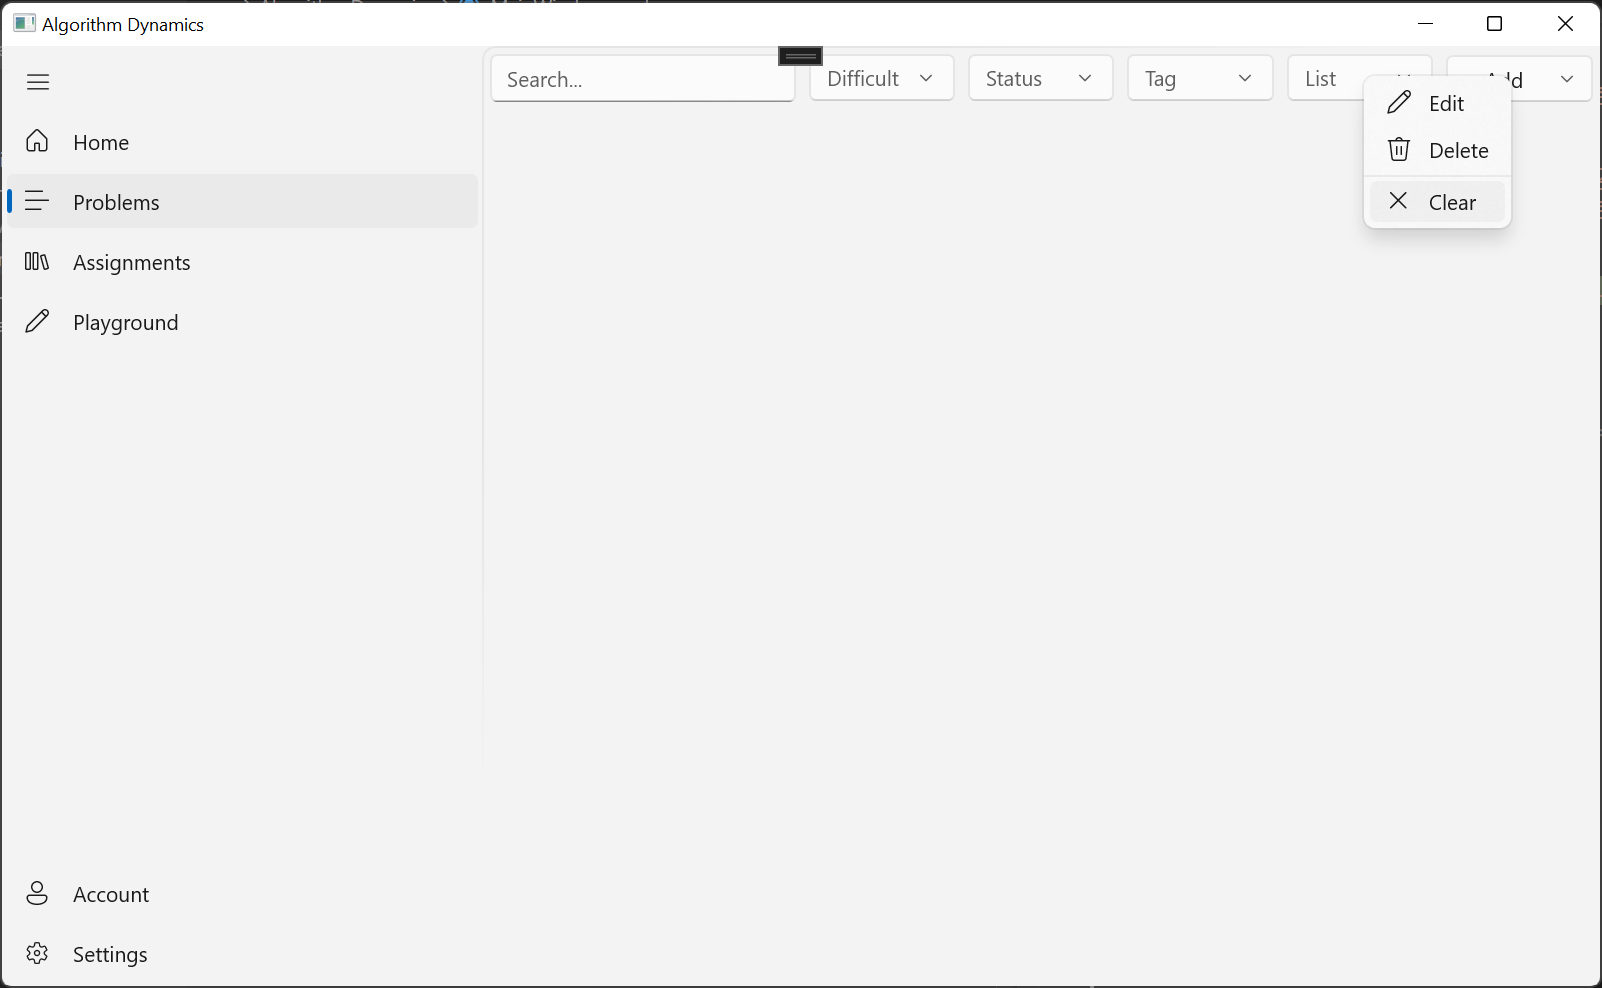
\includegraphics[width=\textwidth, height=\textheight, keepaspectratio]{ProblemsPage-ListComboBox-FlyoutMenu}

But there is a potential issue with the current implementation. When I right-click the list ComboBox, the menu flyout will show up even when no list is selected. Clear the box does not result in any problem because it is empty anyway, but in the future, when the edit and delete function is implemented, attempting to edit or delete an empty list will cause a problem. So I need to change the logic of the menu flyout so that it only shows up when there is something selected. I only need to modify the original function, and only show the flyout when the selected index is -1.

\begin{minted}{csharp}
private void ListComboBox_RightTapped(object sender, RightTappedRoutedEventArgs e)
{
    ComboBox comboBox = (ComboBox)sender;
    if (comboBox.SelectedIndex != -1)
    {
        ListMenuFlyout.ShowAt(comboBox, e.GetPosition(comboBox));
    }
}
\end{minted}

Now, the menu flyout does not show up when no list is selected, which fixes a potential issue in the future.

Next, I need to handle the delete and edit event for the list ComboBox. Because the actual database and data structures have not been implemented yet, I will only create the UI for these events and implement their functions later. For the edit event, the content frame should navigate to the edit page. For the delete event, a content dialog will show up to confirm the deletion. I create two procedures to handle these events.

\begin{minted}{csharp}
/// <summary>
/// Navigate to the edit ProblemList page
/// </summary>
/// <param name="sender"></param>
/// <param name="e"></param>
/// <exception cref="NotImplementedException"></exception>
private void EditProblemList(object sender, RoutedEventArgs e)
{
    // TODO Navigate to edit page
    throw new NotImplementedException();
}

/// <summary>
/// Show a content dialog to confirm the deletion of a ProblemList
/// </summary>
/// <param name="sender"></param>
/// <param name="e"></param>
/// <exception cref="NotImplementedException"></exception>
private async void DeleteProblemList(object sender, RoutedEventArgs e)
{
    ContentDialog dialog = new ContentDialog();
    dialog.Title = "Delete Problem List";
    dialog.PrimaryButtonText = "Delete";
    dialog.CloseButtonText = "Cancel";
    dialog.Content = $"Are you sure that you want to permanently delete {ListComboBox.SelectedItem}?";
    dialog.DefaultButton = ContentDialogButton.Close;
    dialog.XamlRoot = this.Content.XamlRoot;
    var result = await dialog.ShowAsync();
    if (result == ContentDialogResult.Primary)
    {
        // TODO Delete the selected problem list
        throw new NotImplementedException();
    }
}
\end{minted}

Now, when I click the delete button, a popup shows up correctly to confirm deletion.

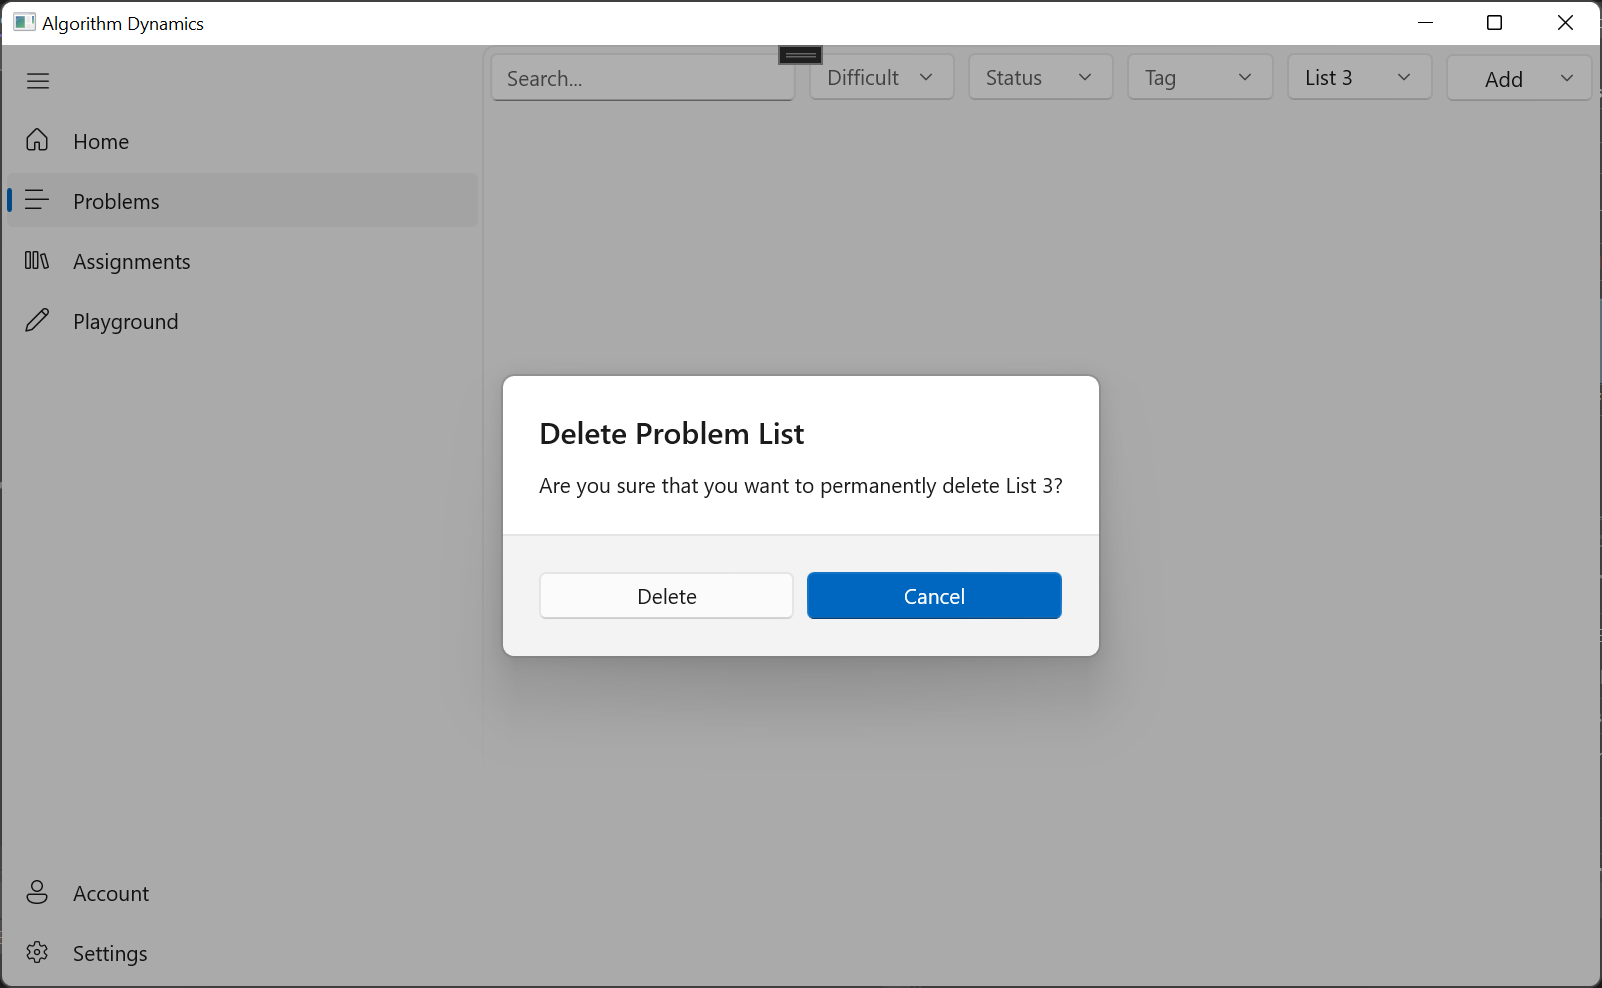
\includegraphics[width=\textwidth, height=\textheight, keepaspectratio]{ProblemsPage-ContentDialog}

I then implement the problem list below the toolbar. I use a \code{ListView} to display the problem list. Similarly, I bind the data source to a variable Problems which contains a list of Problem. For each problem, its name, difficulty, status and tags are displayed.

\begin{minted}{xml}
<ListView x:Name="ProblemsListView"
    Grid.Row="1"
    SelectionMode="Extended"
    Width="auto"
    ItemsSource="{x:Bind Problems, Mode=OneWay}">
    <ListView.ItemContainerStyle>
        <Style TargetType="ListViewItem">
            <Setter Property="HorizontalContentAlignment" Value="Stretch"/>
        </Style>
    </ListView.ItemContainerStyle>
    <ListView.ItemTemplate>
        <DataTemplate x:DataType="local:Problem">
            <Grid>
                <Grid.ColumnDefinitions>
                    <ColumnDefinition Width="2*"/>
                    <ColumnDefinition Width="*"/>
                    <ColumnDefinition Width="*"/>
                    <ColumnDefinition Width="2*"/>
                    <ColumnDefinition Width="*"/>
                </Grid.ColumnDefinitions>
                <TextBlock
                    Text="{x:Bind Name}"
                    Grid.Column="0"
                    HorizontalAlignment="Left"
                    VerticalAlignment="Center"
                    Margin="4 0 0 0"/>
                <TextBlock
                    Text="{x:Bind Difficulty}"
                    Grid.Column="1"
                    HorizontalAlignment="Left"
                    VerticalAlignment="Center"
                    Margin="10 0 0 0"/>
                <TextBlock
                    Text="{x:Bind Status}"
                    Grid.Column="2"
                    HorizontalAlignment="Left"
                    VerticalAlignment="Center"
                    Margin="14 0 0 0"/>
                <TextBlock
                    Text="{x:Bind Tags}"
                    Grid.Column="3"
                    HorizontalAlignment="Left"
                    VerticalAlignment="Center"
                    TextTrimming="CharacterEllipsis"
                    Margin="17 0 0 0"/>
                <Button
                    Content="Start"
                    Grid.Column="4"
                    HorizontalAlignment="Stretch"
                    Margin="12 0 0 0"/>
            </Grid>
        </DataTemplate>
    </ListView.ItemTemplate>
</ListView>
\end{minted}

Because the data structure for Problem has not been implemented yet, I create a sample class for the Problem. It only contains the four attributes that matters and a constructor to initialize the values.

\begin{minted}{csharp}
public class Problem
{
    public Problem(string name, string difficulty, string status, string tags)
    {
        Name = name;
        Difficulty = difficulty;
        Status = status;
        Tags = tags;
    }

    public string Name { get; set; }
    public string Difficulty { get; set; }
    public string Status { get; set; }
    public string Tags { get; set; }
}
\end{minted}

I create a ObserableCollection for the list of Problem and add some sample data to it.

\begin{minted}{csharp}
public ObservableCollection<Problem> Problems = new();
public ProblemsPage()
{
    InitializeComponent();
    Problems.Add(new Problem("Problem 1", "Easy", "Todo", "Tag"));
    Problems.Add(new Problem("Problem 2", "Easy", "Attempted", "Tag"));
    Problems.Add(new Problem("Problem 3", "Easy", "Done", "Tag"));
    Problems.Add(new Problem("Problem 4", "Medium", "Todo", "Tag"));
    Problems.Add(new Problem("Problem 5", "Medium", "Attempted", "Tag"));
    Problems.Add(new Problem("Problem 6", "Medium", "Done", "Tag"));
    Problems.Add(new Problem("Problem 7", "Hard", "Todo", "Tag"));
    Problems.Add(new Problem("Problem 8", "Hard", "Attempted", "Tag"));
    Problems.Add(new Problem("Problem 9", "Hard", "Done", "Tag"));
    Problems.Add(new Problem("Problem 10", "Hard", "Todo", "Tag"));
}
\end{minted}

The problem list shows up with the correct data.

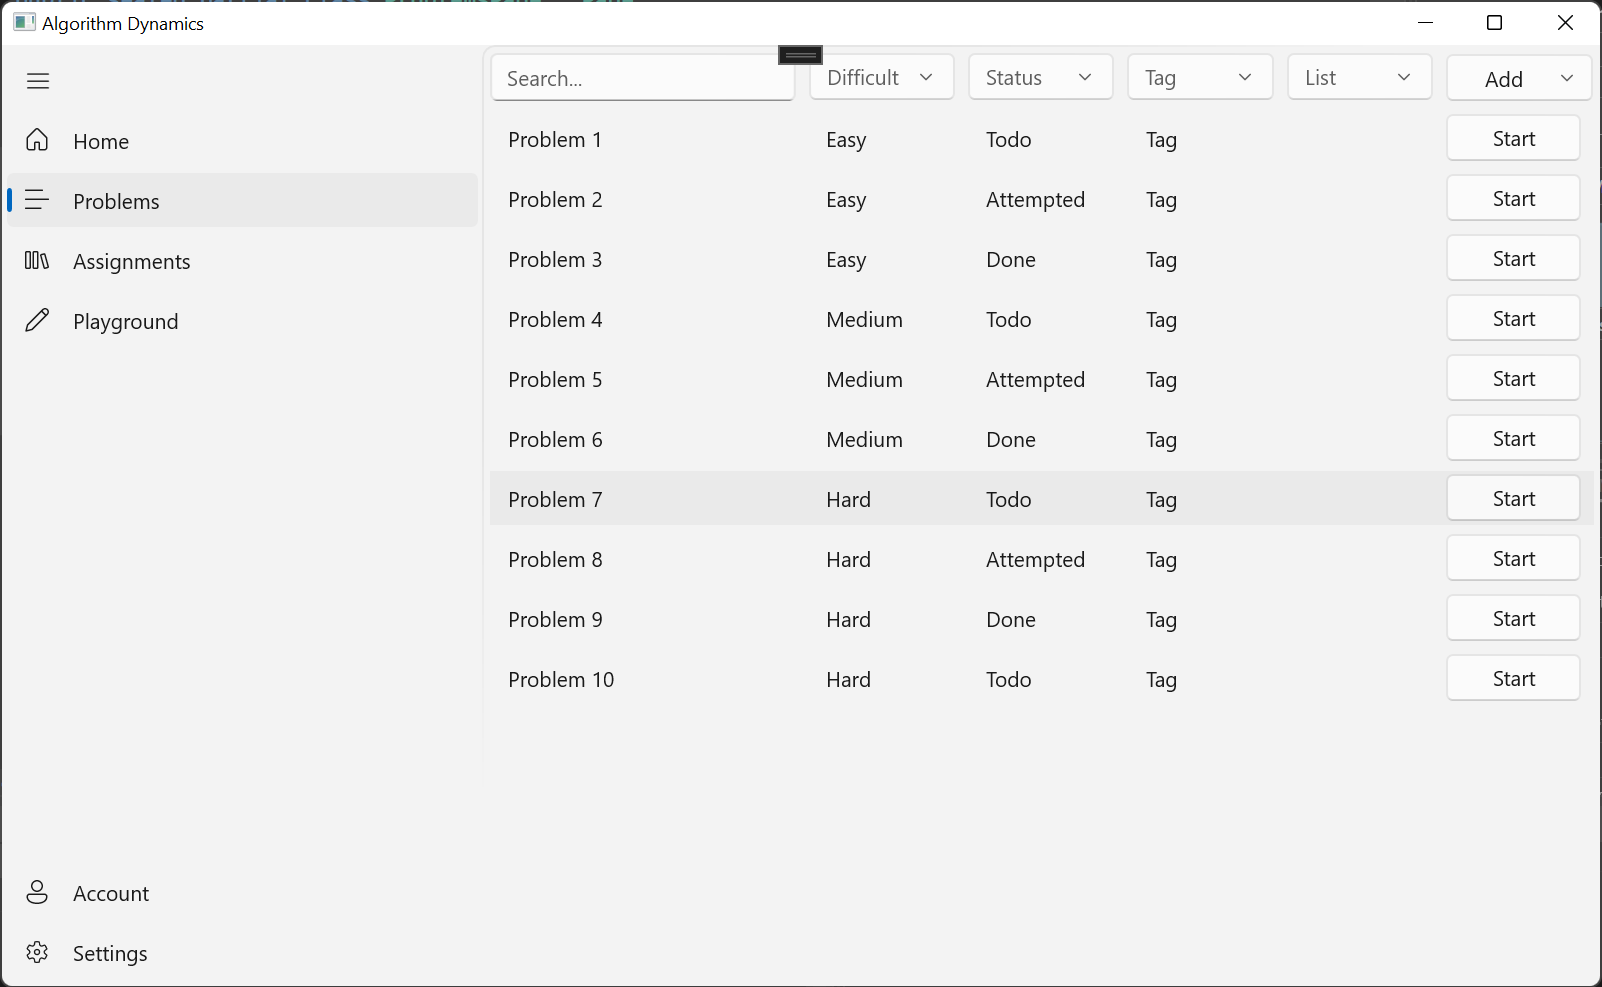
\includegraphics[width=\textwidth, height=\textheight, keepaspectratio]{ProblemsPage-ProblemList}

I need to add a flyout menu for the problem list to allow the user to edit and delete problems when right clicking the list. When only one problem is selected, the user can edit it or delete it. When multiple problems are selected, the user can delete all of them or create a problem list from them.

\begin{minted}{xml}
<ListView.Resources>
    <MenuFlyout x:Name="SingleSelectedMenuFlyout">
        <MenuFlyout.Items>
            <MenuFlyoutItem 
                Text="Edit"
                Icon="Edit"/>
            <MenuFlyoutItem 
                Text="Delete"
                Icon="Delete"/>
        </MenuFlyout.Items>
    </MenuFlyout>
    <MenuFlyout x:Name="MultipleSelectedMenuFlyout">
        <MenuFlyout.Items>
            <MenuFlyoutItem 
                Text="Create Problem List..."
                Icon="Add"/>
            <MenuFlyoutItem 
                Text="Delete"
                Icon="Delete"/>
        </MenuFlyout.Items>
    </MenuFlyout>
</ListView.Resources>
\end{minted}


\begin{minted}{csharp}
/// <summary>
/// Show flyout when the user right tapped the ProblemListView
/// When one problem is selected, show the SingleSelectedMenuFlyout
/// When mutiple problems are selected, show the MultipleSelectedMenuFlyout
/// </summary>
/// <param name="sender"></param>
/// <param name="e"></param>
private void ProblemsListView_RightTapped(object sender, RightTappedRoutedEventArgs e)
{
    ListView listView = (ListView)sender;
    if (listView.SelectedItems.Count == 1)
    {
        SingleSelectedMenuFlyout.ShowAt(listView, e.GetPosition(listView));
    }
    else if (listView.SelectedItems.Count > 1)
    {
        MultipleSelectedMenuFlyout.ShowAt(listView, e.GetPosition(listView));
    }
}
\end{minted}

The corresponding menu flyout can show up correctly based on the selection.

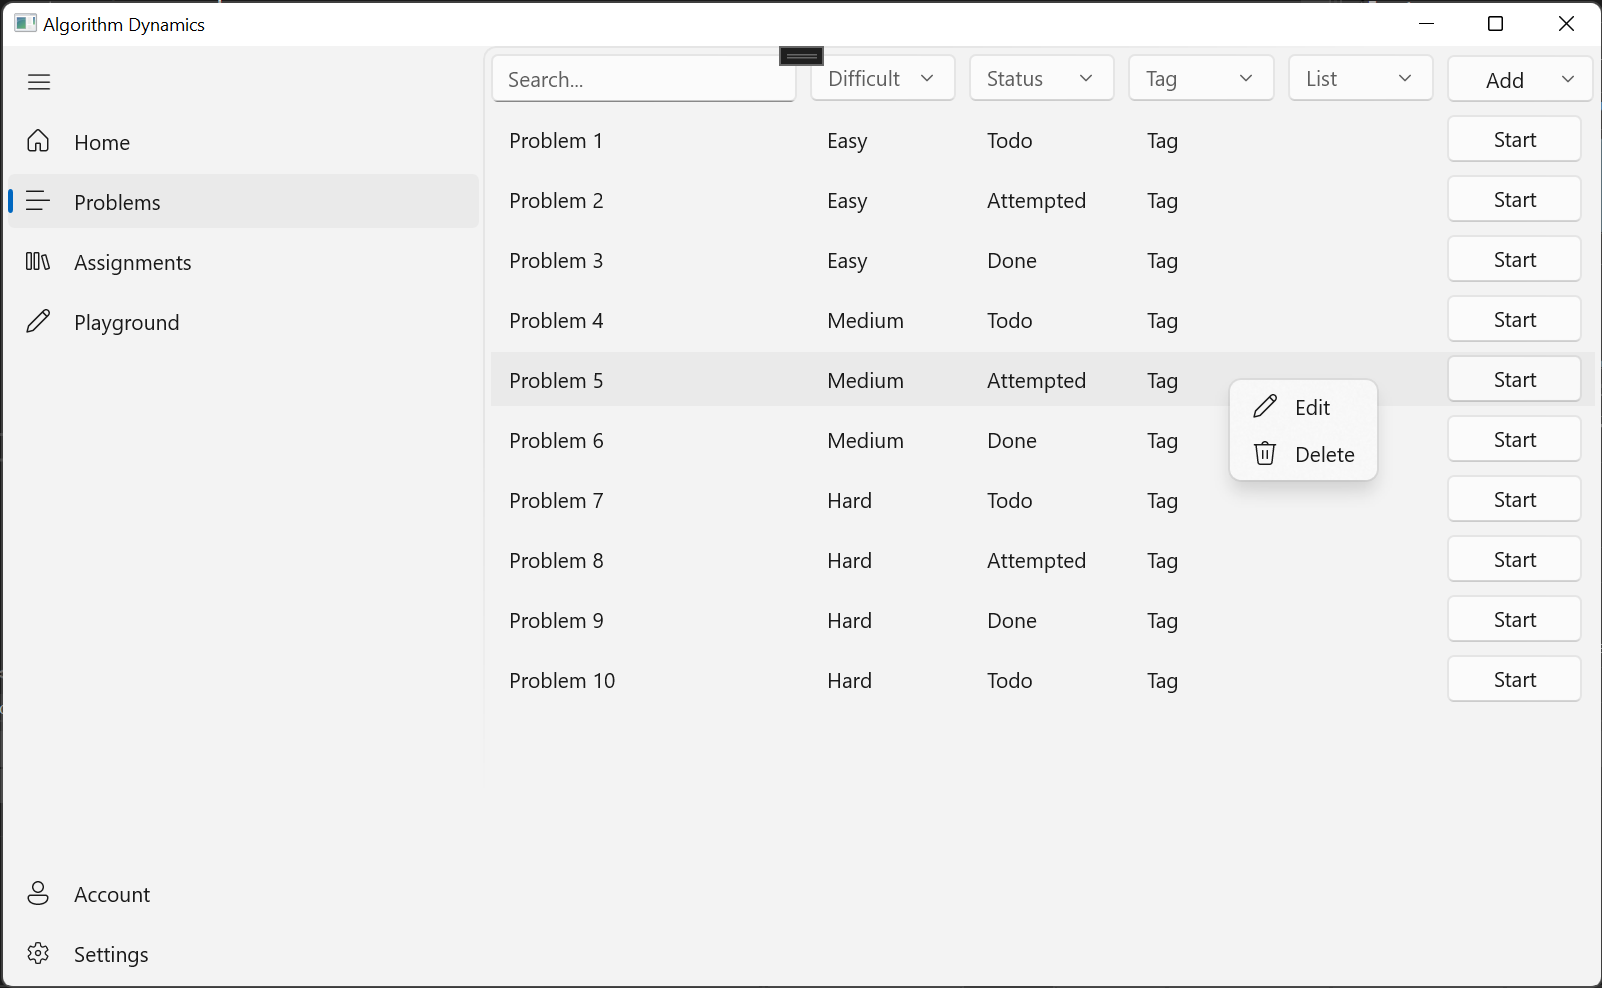
\includegraphics[width=\textwidth, height=\textheight, keepaspectratio]{ProblemsPage-SingleSelected-Flyout}

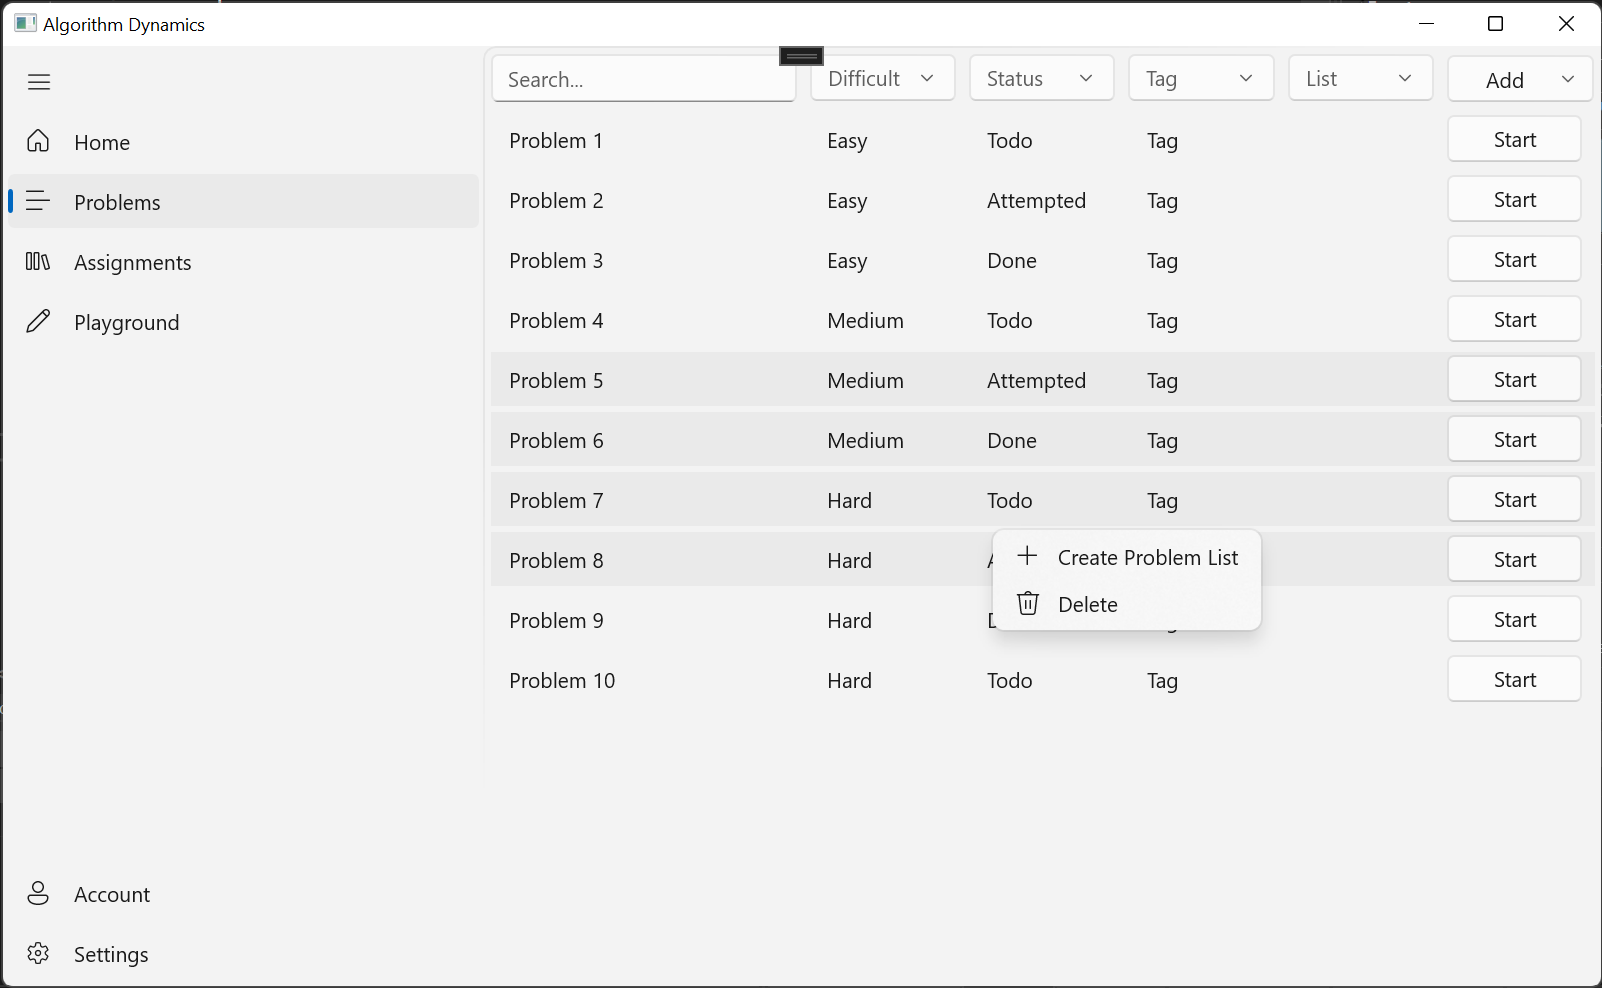
\includegraphics[width=\textwidth, height=\textheight, keepaspectratio]{ProblemsPage-MultipleSelected-Flyout}

Similarly, I can add the delete content dialog for these flyouts and leave the edit and create new problem list feature in the future.

\begin{minted}{csharp}
/// <summary>
/// Edit the selected Problem
/// Navigate to the EditProblemPage
/// </summary>
/// <param name="sender"></param>
/// <param name="e"></param>
private void EditProblem(object sender, RoutedEventArgs e)
{
    // TODO Navigate to the EditProblemPage
    throw new NotImplementedException();
}

/// <summary>
/// Show a content dialog to confirm the deletion of a Problem
/// </summary>
/// <param name="sender"></param>
/// <param name="e"></param>
/// <exception cref="NotImplementedException"></exception>
private async void DeleteProblem(object sender, RoutedEventArgs e)
{
    ContentDialog dialog = new ContentDialog();
    dialog.Title = "Delete Problem";
    dialog.PrimaryButtonText = "Delete";
    dialog.CloseButtonText = "Cancel";
    dialog.Content = $"Are you sure that you want to permanently delete {(ProblemsListView.SelectedItem as Problem).Name}?";
    dialog.DefaultButton = ContentDialogButton.Close;
    dialog.XamlRoot = this.Content.XamlRoot;
    var result = await dialog.ShowAsync();
    if (result == ContentDialogResult.Primary)
    {
        // TODO Delete the selected problem
        throw new NotImplementedException();
    }
}

/// <summary>
/// Create a new ProblemList from multiple selected items
/// Navigate to the CreateProblemListPage
/// </summary>
/// <param name="sender"></param>
/// <param name="e"></param>
/// <exception cref="NotImplementedException"></exception>
private void CreateProblemList(object sender, RoutedEventArgs e)
{
    // TODO Navigate to the CreateProblemList
    throw new NotImplementedException();
}

/// <summary>
/// Show a content dialog to confirm the deletion of Problems
/// </summary>
/// <param name="sender"></param>
/// <param name="e"></param>
/// <exception cref="NotImplementedException"></exception>
private async void DeleteProblems(object sender, RoutedEventArgs e)
{
    ContentDialog dialog = new ContentDialog();
    dialog.Title = "Delete Problem";
    dialog.PrimaryButtonText = "Delete";
    dialog.CloseButtonText = "Cancel";
    dialog.Content = $"Are you sure that you want to permanently delete these {ProblemsListView.SelectedItems.Count} Problems?";
    dialog.DefaultButton = ContentDialogButton.Close;
    dialog.XamlRoot = this.Content.XamlRoot;
    var result = await dialog.ShowAsync();
    if (result == ContentDialogResult.Primary)
    {
        // TODO Delete the selected problems
        throw new NotImplementedException();
    }
}
\end{minted}

Finally, for the ProblemsPage, I need to handle the searh query. The ProblemListView needs to be updated when different search queries are entered in the toolbar. I create a \code{Search} procedure to handle the searc event. When the user select an option in the ComboBoxes, or enter the search box, the \code{Search} procedure will be called. All data will be passed to a \code{Query} function that returns searching result. For now, because the database is not implemented, I will just return the query. The \code{Query} function will be implemented in the future.

\begin{minted}{csharp}
/// <summary>
/// Search the problem lists that under conditions
/// </summary>
/// <param name="sender"></param>
/// <param name="args"></param>
private void Search(object sender, object args)
{
    var keywords = ProblemsSearchBox.Text;
    var difficulty = DifficultyComboBox.SelectedValue?.ToString();
    var status = StatusComboBox.SelectedValue?.ToString();
    var tag = TagComboBox.SelectedValue?.ToString();
    var list = ListComboBox.SelectedValue?.ToString();
    // TODO Query(keywords, difficulty, status, tag, list);
    Problems.Clear();
    Problems.Add(new Problem(keywords, difficulty, status, tag));
}
\end{minted}

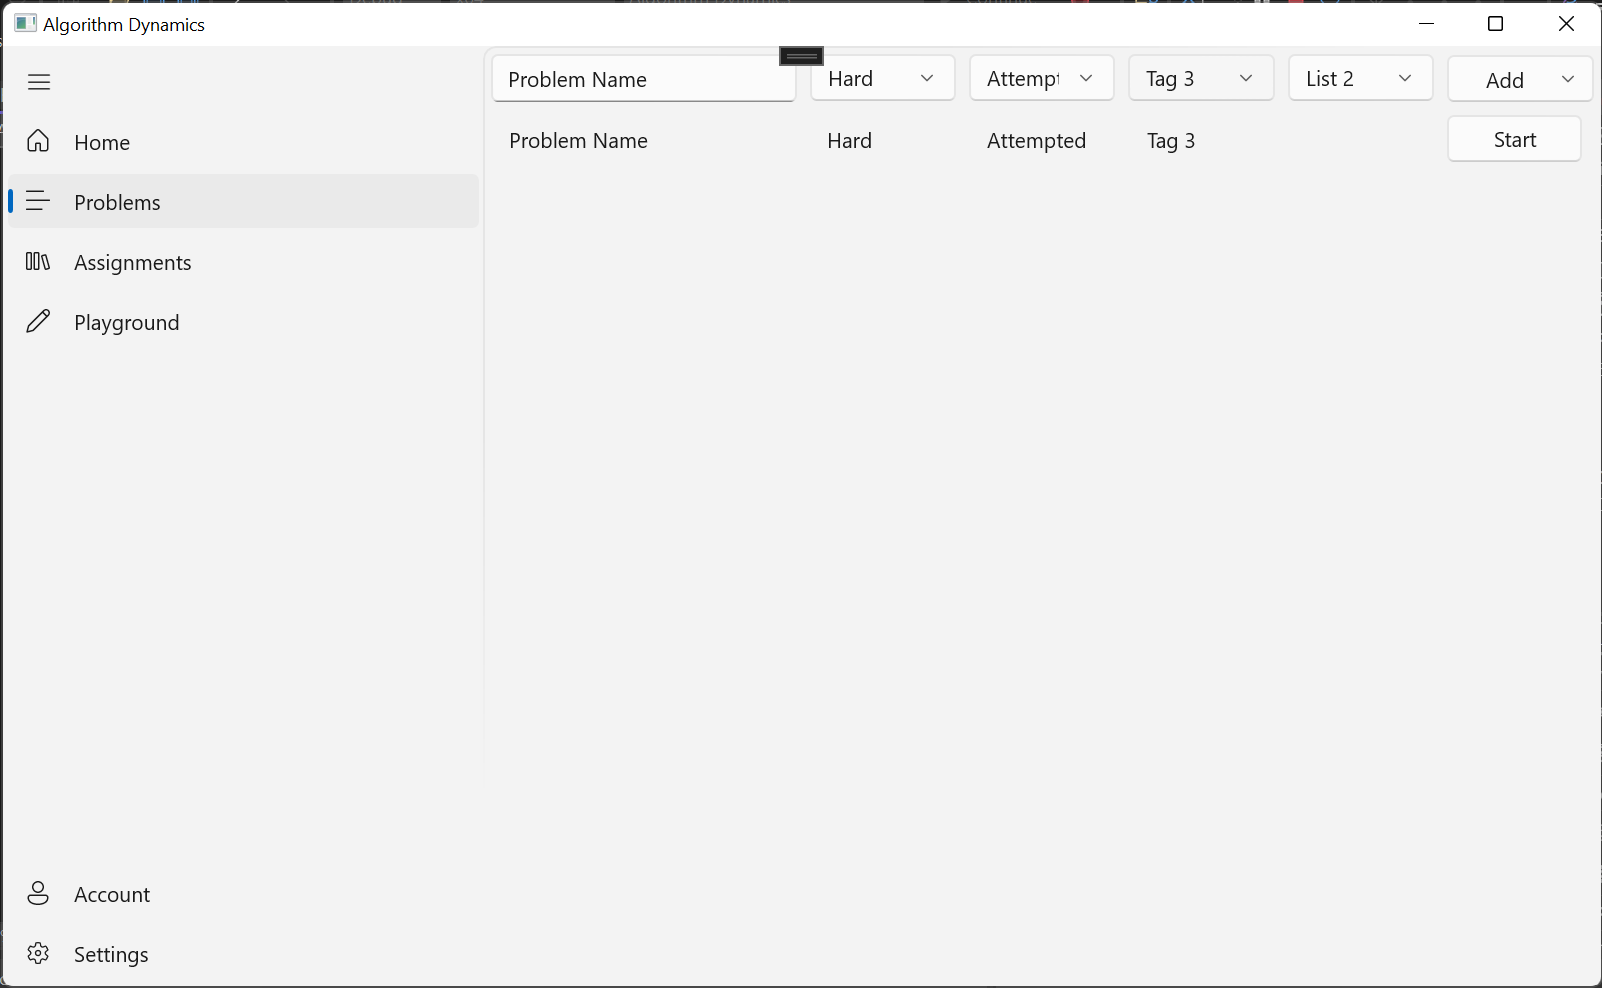
\includegraphics[width=\textwidth, height=\textheight, keepaspectratio]{ProblemsPage-Search}

The correct search result is returned and the search result is updated correctly when different search conditions are selected.

\subsubsection{Testing and validation}

\begin{tabulary}{\linewidth}{|L|l|L|}
    \hline
    Test & Result & Remark \\
    \hline
    Does it load & Pass & \\
    \hline
    Does the toolbar display correctly & Pass & \\
    \hline
    Does the toolbar interact correctly & Pass & \\
    \hline
    Does the toolbar return the correct search result & Failed & The search algorithm will be implemented after the database and data structure is ready in the future milestones. \\
    \hline
    Does the add button work & Failed & The data import and create new problem function will be implemented after the CreateNewProblemPage and the data import function is implemented. \\
    \hline
    Does the problem list show up correct & Pass & \\
    \hline
    Does the start button work & Failed & The start button will be implemented after the coding page is implemented. \\
    \hline
    Does the selection and menu flyout work & Failed & The delete and edit button will be implemented after the database is ready. \\
    \hline
\end{tabulary}

The ProblemsPage is partially implemented with many todos left for the future. But in this iteration, it is good to go as all UI elements are ready. I will move on to the PlaygroundPage and CodingPage next.

\subsubsection{Stakeholder feedback}

TODO: Copy problem

\subsection{Create the PlaygroundPage}

\subsubsection{Implementation}

The main component in the PlaygroundPage is the Code Editor. Because the CodingPage will need to use the Code Editor as well, so I will set the Code Editor as a custom control so it can be reused later.

The Code Editor needs to support line number, syntax highlighting, and other editing features. It is too complex for this project to implement all of these by hand. So I will use a third-party library to achieve that. I am using the \href{https://microsoft.github.io/monaco-editor/}{Monaco Editor} for this purpose.

I create a custom control for the editor so I can reuse it later in different pages easily.

\begin{minted}{xml}
<UserControl
    x:Class="Algorithm_Dynamics.Controls.CodeEditor"
    xmlns="http://schemas.microsoft.com/winfx/2006/xaml/presentation"
    xmlns:x="http://schemas.microsoft.com/winfx/2006/xaml"
    xmlns:local="using:Algorithm_Dynamics.Controls"
    xmlns:d="http://schemas.microsoft.com/expression/blend/2008"
    xmlns:mc="http://schemas.openxmlformats.org/markup-compatibility/2006"
    mc:Ignorable="d">

    <TextBlock Text="CodeEditor"/>
</UserControl>
\end{minted}

\begin{minted}{csharp}
using Microsoft.UI.Xaml.Controls;

namespace Algorithm_Dynamics.Controls
{
    public sealed partial class CodeEditor : UserControl
    {
        public CodeEditor()
        {
            InitializeComponent();
        }
    }
}
\end{minted}

I import the control in the PlaygroundPage to verify its working.

\begin{minted}{xml}
<Page
    x:Class="Algorithm_Dynamics.Pages.PlaygroundPage"
    xmlns="http://schemas.microsoft.com/winfx/2006/xaml/presentation"
    xmlns:x="http://schemas.microsoft.com/winfx/2006/xaml"
    xmlns:local="using:Algorithm_Dynamics.Pages"
    xmlns:controls="using:Algorithm_Dynamics.Controls"
    xmlns:d="http://schemas.microsoft.com/expression/blend/2008"
    xmlns:mc="http://schemas.openxmlformats.org/markup-compatibility/2006"
    mc:Ignorable="d"
    Background="{ThemeResource ApplicationPageBackgroundThemeBrush}">

    <Grid>
        <controls:CodeEditor/>
    </Grid>
</Page>
\end{minted}

Now, when I run the application and navigate to the PlaygroundPage I can see the Code Editor is displayed correctly.

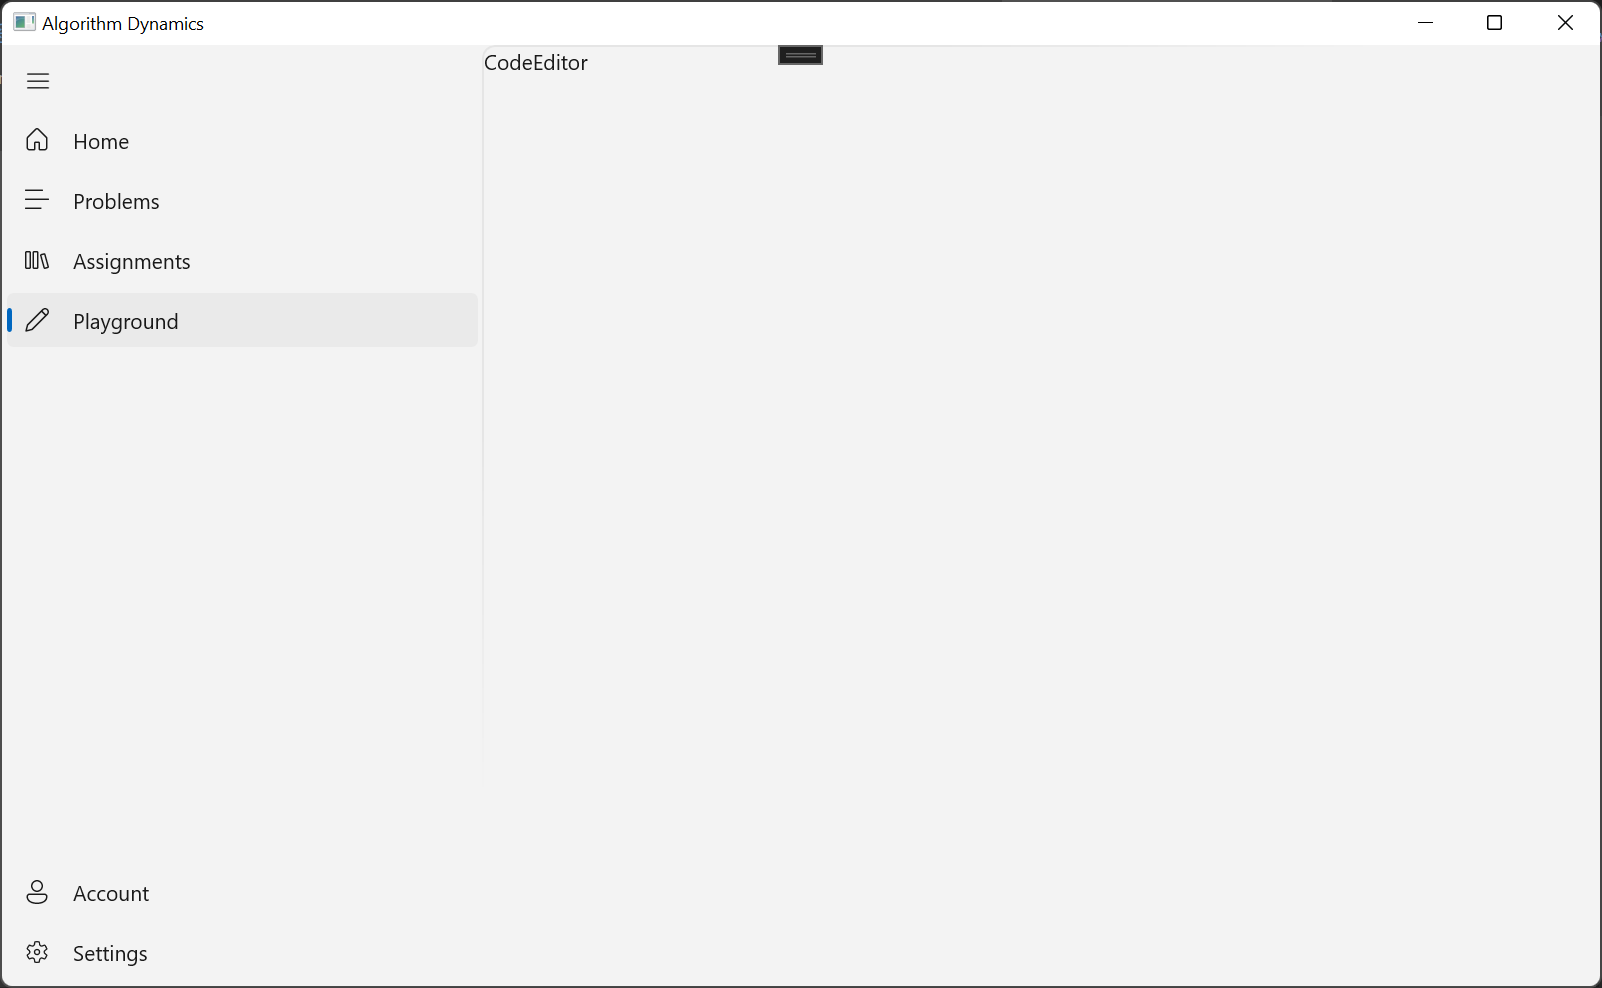
\includegraphics[width=\textwidth, height=\textheight, keepaspectratio]{CodeEditorControl}

The Monaco Editor is a web application, which means it needs to run in a browser. To use it, I need to use WebView2 component to load a HTML file, and initialize the Monaco Editor inside that webpage. The WebView2 control launches a Chromium instance and allows me to integrate webpages inside my app. I use the WebView2 control to load the HTML file. Before I create the webpage for the Monaco Editor, I place the WebView2 control and test it out.

\begin{minted}{xml}
<WebView2 
    x:Name="WebView"
    HorizontalAlignment="Stretch"
    VerticalAlignment="Stretch"
    Source="https://ocr.org.uk"/>
\end{minted}

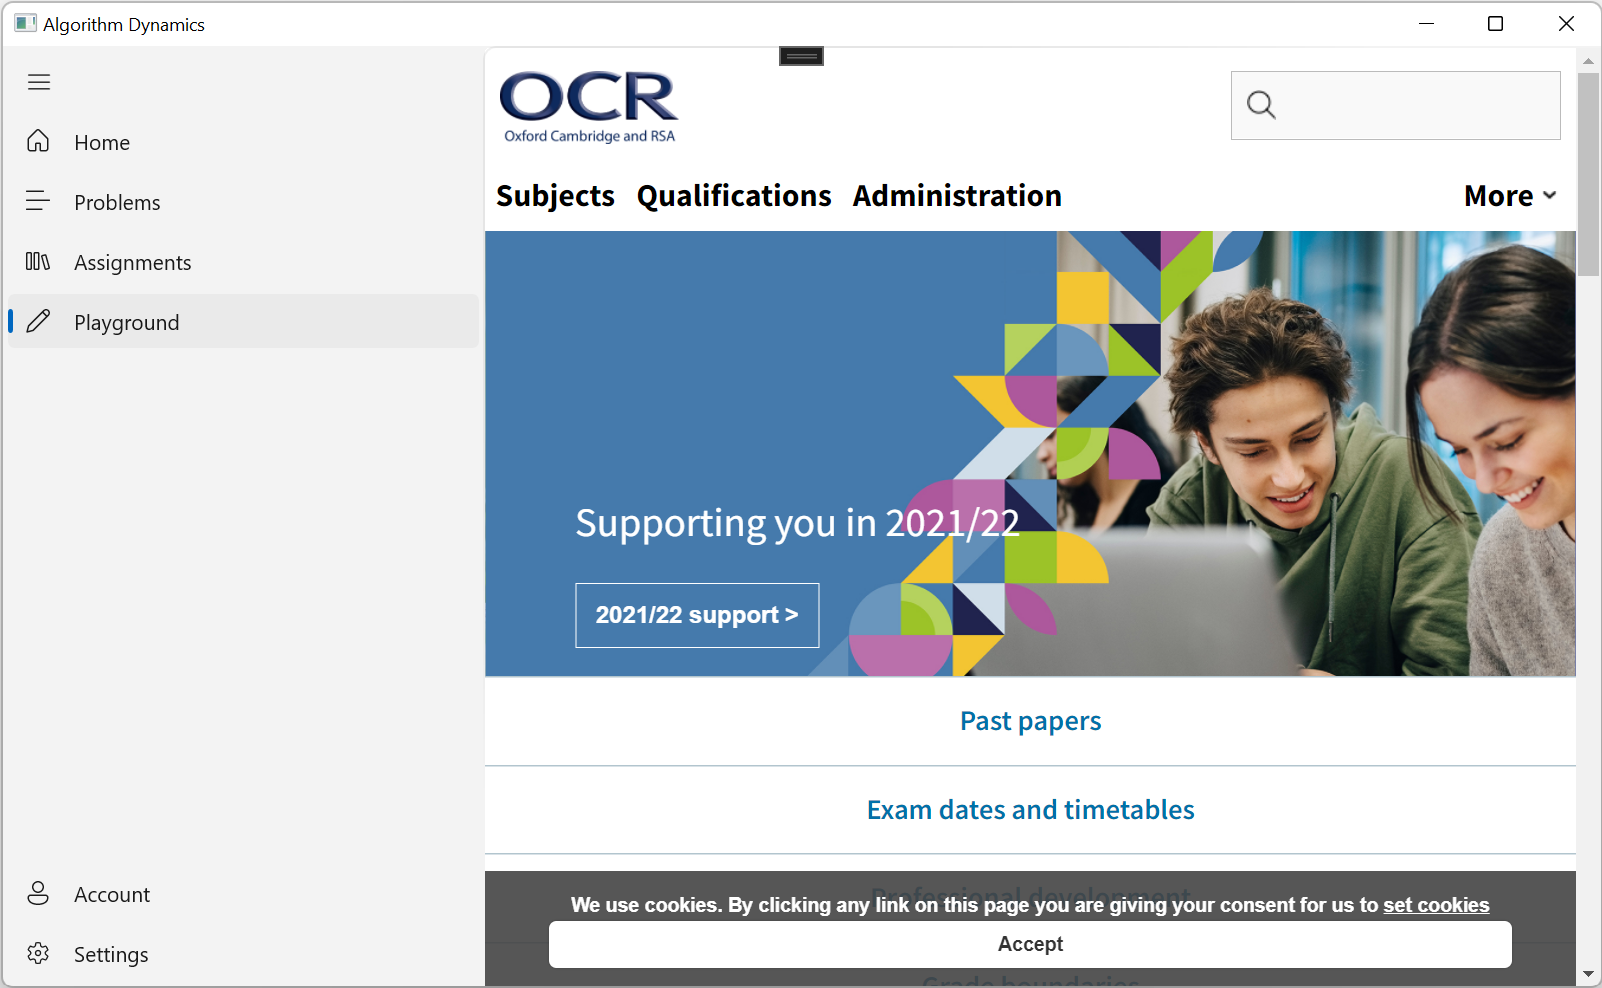
\includegraphics[width=\textwidth, height=\textheight, keepaspectratio]{PlaygroundPage-WebView2-Webpage}

I set the source of the WebView2 control to the offcial website of OCR, and it loads up correctly. Now I can start working on the webpage for the editor. To load a local HTML file, I need to set a mapping relationship between a URL space and a local folder.

\begin{minted}{csharp}
/// <summary>
/// Initialize the WebView control and load Editor.html
/// </summary>
async void InitializeWebViewAsync()
{
    // Ensure the CoreWebView2 is loaded
    await WebView.EnsureCoreWebView2Async();

    // Set the mapping
    StorageFolder AssetsDirectory = await Package.Current.InstalledLocation.GetFolderAsync(@"Assets");
    WebView.CoreWebView2.SetVirtualHostNameToFolderMapping(
        "localeditor.algorithmdynamics.com",
        AssetsDirectory.Path,
        CoreWebView2HostResourceAccessKind.Allow
    );

    // Load Editor.html
    WebView.Source = new Uri("http://localeditor.algorithmdynamics.com/Editor.html");
}
\end{minted}

Now I can load Editor.html under the Assets folder. I use a sample HTML file to test it out.

\begin{minted}{html}
<!DOCTYPE html>
<html lang="en">
<head>
    <meta charset="UTF-8">
    <meta http-equiv="X-UA-Compatible" content="IE=edge">
    <meta name="viewport" content="width=device-width, initial-scale=1.0">
    <title>Document</title>
</head>
<body>
    <h1>Hello Editor!</h1>
</body>
</html>
\end{minted}

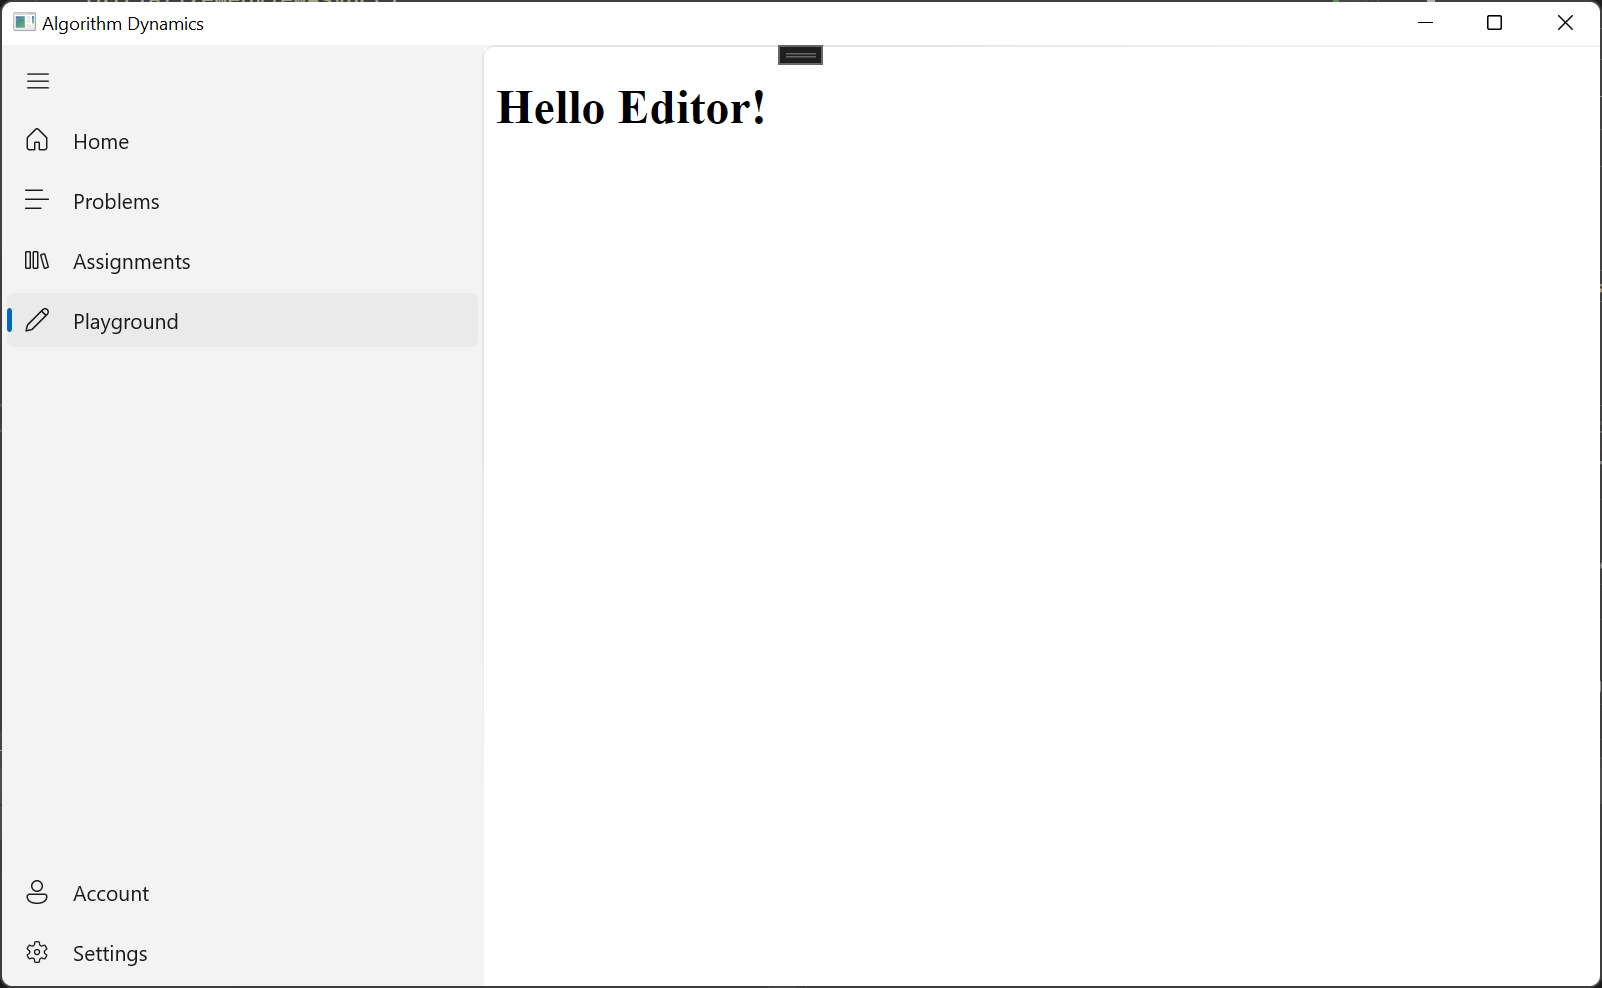
\includegraphics[width=\textwidth, height=\textheight, keepaspectratio]{PlaygroundPage-WebView2-HelloEditor}

The h1 title ``Hello Editor!'' is displayed correctly, which means the local file is loaded as expected. Now I can import the Monaco Editor to the WebView2 control.

\begin{minted}{html}
<body>
    <div id="container" style="width:800px;height:600px;border:1px solid grey"></div>

    <script src="monaco-editor/min/vs/loader.js"></script>
    <script>
        require.config({ paths: { vs: 'monaco-editor/min/vs' } });
        require(['vs/editor/editor.main'], () => {
            window.editor = monaco.editor.create(document.getElementById('container'), {
                value: ['function x() {', '\tconsole.log("Hello Editor!");', '}'].join('\n'),
                language: 'javascript'
            });
        });
    </script>
</body>
\end{minted}

I add a container in the body to host the instance of the editor. Then I write some JavaScript code to import the editor and initialize it with a sample code.

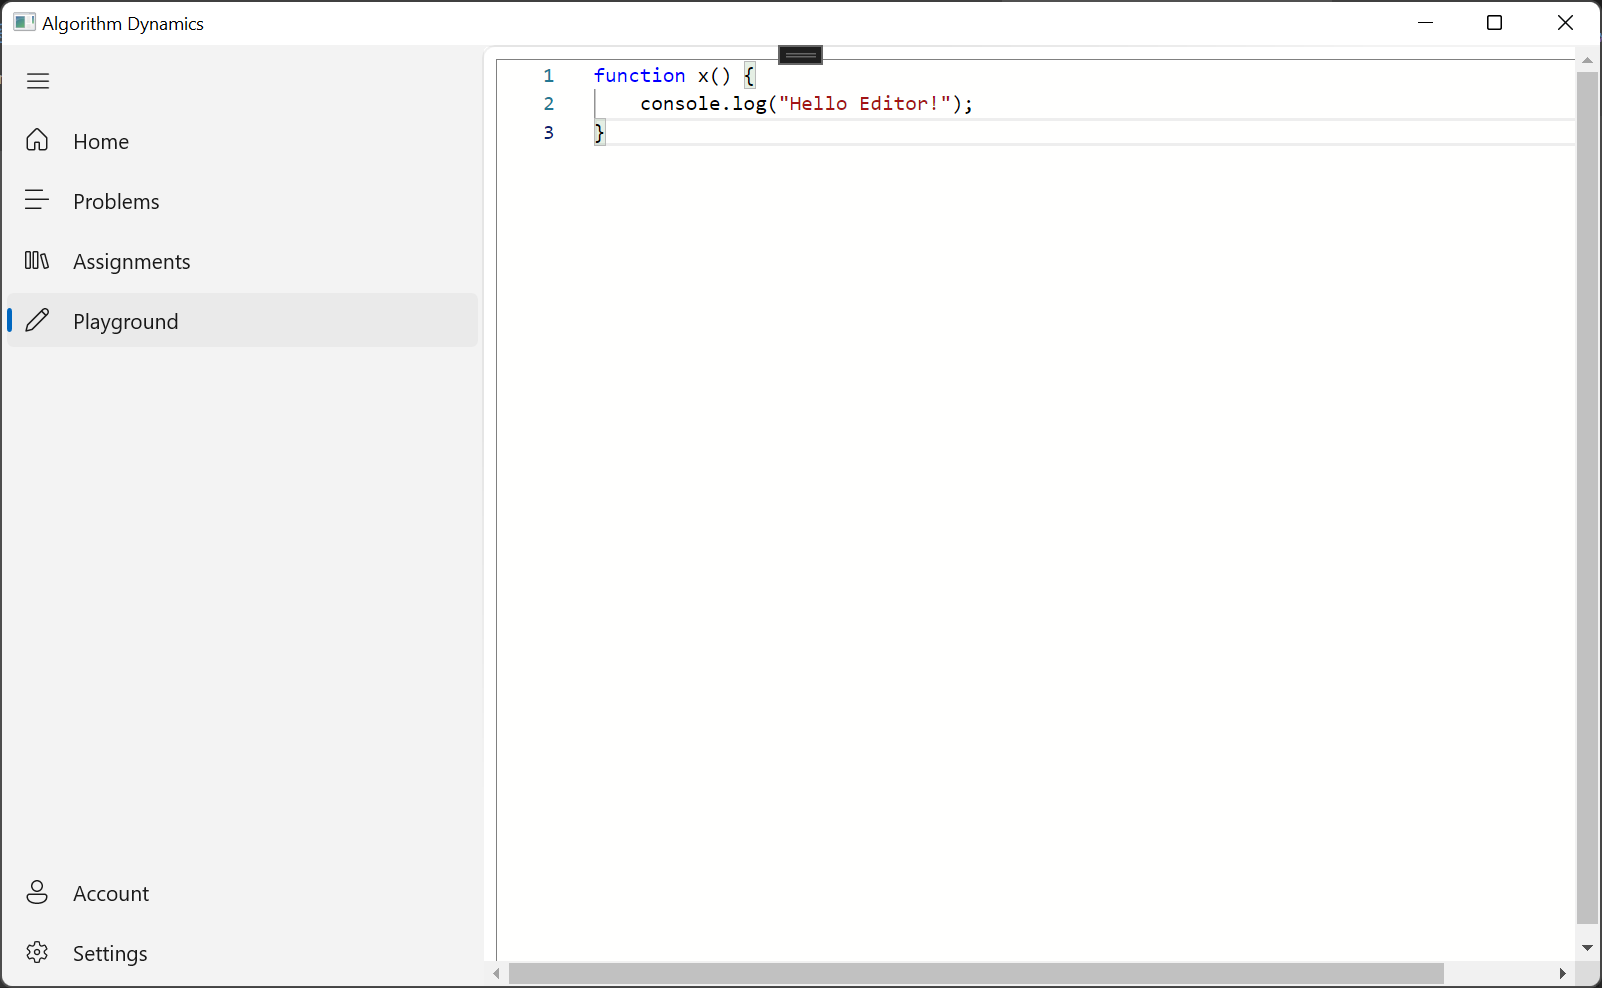
\includegraphics[width=\textwidth, height=\textheight, keepaspectratio]{PlaygroundPage-WebView2-EditorLoaded}

The editor is now loaded correctly with the sample code. I can type in the editor and utlize all powerful functions of the Monaco Editor.

But I find that the editor has a fixed height and width. On a small screen like the screen shot, you can see the scroll bars. And on a larger display, the editor will not occupy the entire screen. I need to adjust its style to make it responsive.

I add some CSS code to set the height and width of the editor to 100\%.

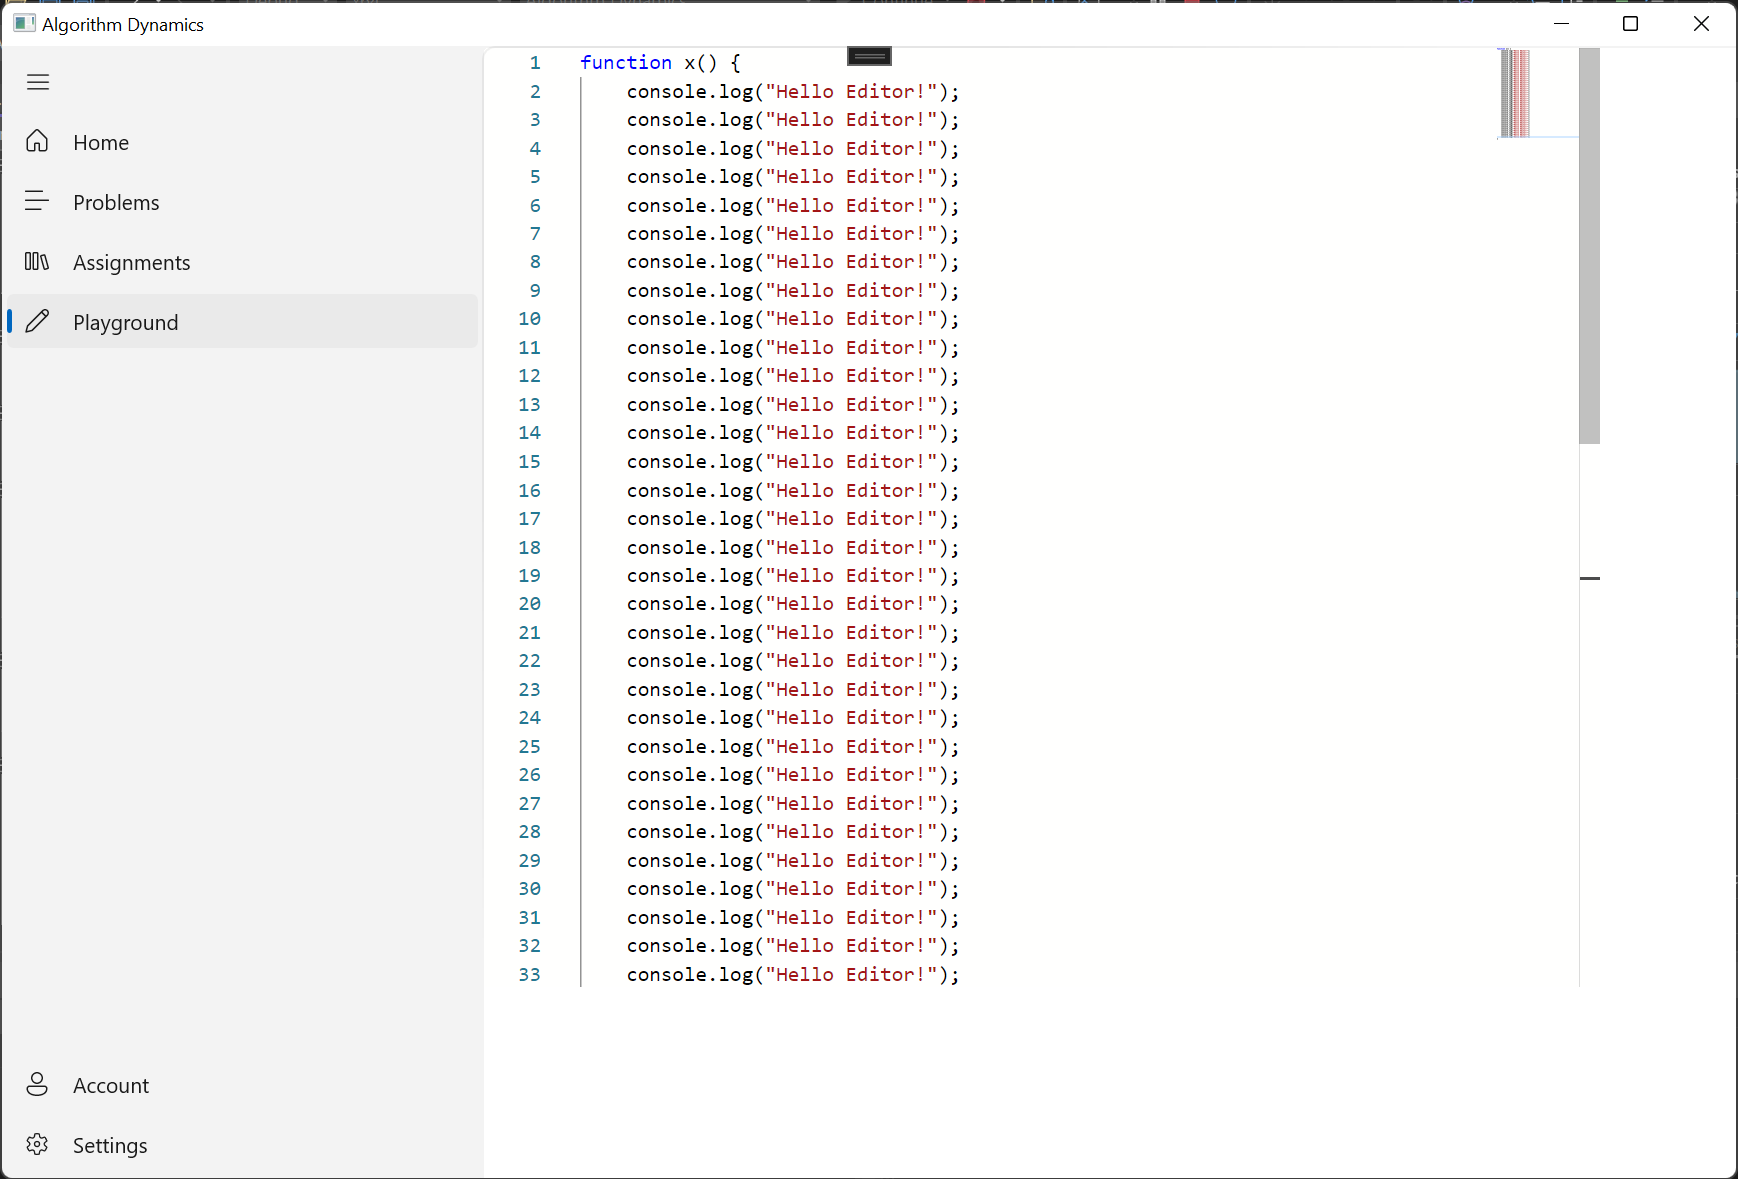
\includegraphics[width=\textwidth, height=\textheight, keepaspectratio]{PlaygroundPage-WebView2-ResizeFailed}

Now, the scroll bars are gone. But when I resize the window, the editor still does not follow the window size. After reading the documentation of the Monaco Editor, I find out that I need to manually call the \code{editor.layout()} function to recalculate the editor size.

\begin{minted}{html}
<script>
    window.addEventListener("resize", () => editor.layout());
</script>
\end{minted}

By adding the event handler for the window resize event and call the layout function, the editor can now resize correctly according to the window size.

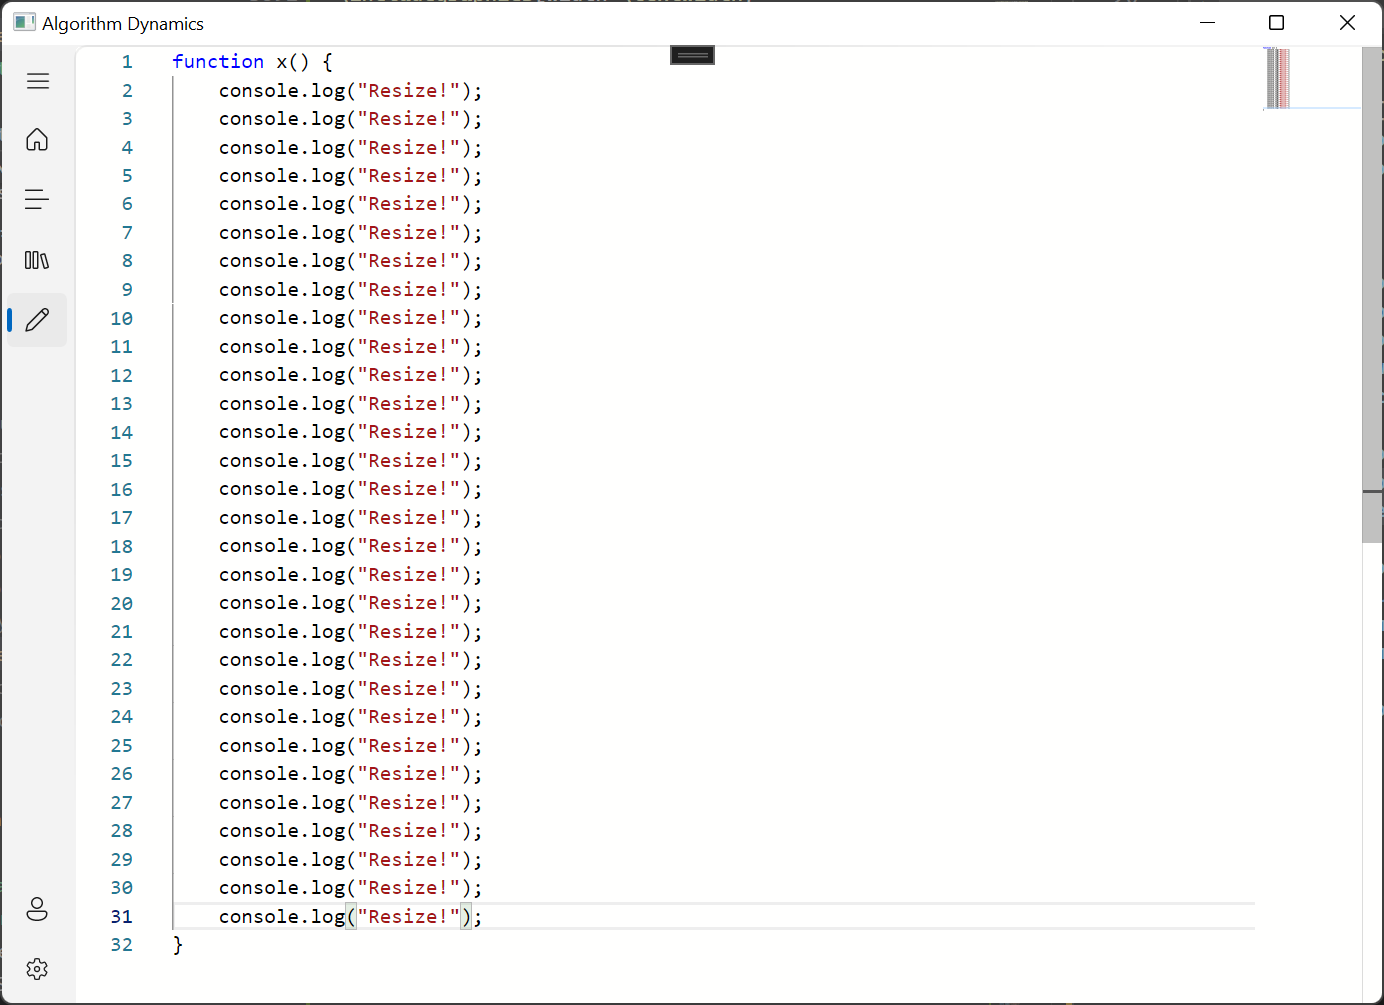
\includegraphics[width=\textwidth, height=\textheight, keepaspectratio]{PlaygroundPage-WebView2-ResizeSuccess}

Before I go any further, I need to first implement the PlaygroundPage, so I have a working environment to test the editor out.

\begin{minted}{xml}
<Page
    x:Class="Algorithm_Dynamics.Pages.PlaygroundPage"
    xmlns="http://schemas.microsoft.com/winfx/2006/xaml/presentation"
    xmlns:x="http://schemas.microsoft.com/winfx/2006/xaml"
    xmlns:local="using:Algorithm_Dynamics.Controls"
    xmlns:controls="using:CommunityToolkit.WinUI.UI.Controls"

    xmlns:d="http://schemas.microsoft.com/expression/blend/2008"
    xmlns:mc="http://schemas.openxmlformats.org/markup-compatibility/2006"
    mc:Ignorable="d"
    Background="{ThemeResource ApplicationPageBackgroundThemeBrush}">

    <Grid>
        <Grid.RowDefinitions>
            <RowDefinition Height="*"/>
            <RowDefinition Height="*"/>
            <RowDefinition Height="auto"/>
        </Grid.RowDefinitions>

        <Grid.ColumnDefinitions>
            <ColumnDefinition Width="*"/>
            <ColumnDefinition Width="*"/>
        </Grid.ColumnDefinitions>

        <!-- ... -->
    </Grid> 
</Page>
\end{minted}

I will use a grid with 3 rows and 2 columns to hold all controls.

\begin{minted}{xml}
<local:CodeEditor
    x:Name="CodeEditor"
    Grid.Row="0"
    Grid.Column="0"
    Grid.RowSpan="2"
    Margin="0 0 8 0"/>

<TextBox
    x:Name="OutputBox"
    Grid.Row="0"
    Grid.Column="1"
    Margin="8 0 0 8"
    PlaceholderText="Output"
    IsSpellCheckEnabled="False"
    AcceptsReturn="True"/>

<TextBox
    x:Name="InputBox"
    Grid.Row="1"
    Grid.Column="1"
    Margin="8 8 0 0"
    PlaceholderText="Input"
    IsSpellCheckEnabled="False"
    AcceptsReturn="True"/>

<Grid
    Grid.Row="2"
    Grid.Column="0">
    <ComboBox
        x:Name="LanguageComboBox"
        SelectedIndex="0"
        VerticalAlignment="Stretch">
        <x:String>Python</x:String>
        <x:String>C</x:String>
        <x:String>C++</x:String>
    </ComboBox>
</Grid>

<Grid
    Grid.Row="2"
    Grid.Column="1"
    Margin="8 0 0 0">
    <Grid.RowDefinitions>
        <RowDefinition Height="auto"/>
        <RowDefinition Height="*"/>
    </Grid.RowDefinitions>
    <Grid.ColumnDefinitions>
        <ColumnDefinition Width="*"/>
        <ColumnDefinition Width="*"/>
    </Grid.ColumnDefinitions>
    <ProgressBar
        Grid.Row="0"
        Grid.Column="0"
        Grid.ColumnSpan="2"
        HorizontalAlignment="Stretch"
        VerticalAlignment="Stretch"
        IsIndeterminate="True"
        ShowPaused="False"
        ShowError="False" />
    <TextBlock
        x:Name="StatusTextBlock"
        Grid.Row="1"
        Grid.Column="0"
        HorizontalAlignment="Left"
        VerticalAlignment="Center"
        Text="Pending"/>
    <Button
        x:Name="RunCodeButton"
        Grid.Row="1"
        Grid.Column="1"
        HorizontalAlignment="Right"
        VerticalAlignment="Stretch"
        Content="Run Code"
        Click="RunCodeButton_Click"/>
</Grid>
\end{minted}

To allow different sections to be resizeable, I add two grid splitters to the grid.

\begin{minted}{xml}
<controls:GridSplitter
    HorizontalAlignment="Left"
    Grid.Column="1"
    Grid.RowSpan="2"
    Width="16">
    <controls:GridSplitter.RenderTransform>
        <TranslateTransform X="-8" />
    </controls:GridSplitter.RenderTransform>
</controls:GridSplitter>

<controls:GridSplitter
    VerticalAlignment="Top"
    Grid.Row="1"
    Grid.Column="1"
    Grid.ColumnSpan="1"
    Margin="8 0 0 0"
    Height="16">
    <controls:GridSplitter.RenderTransform>
        <TranslateTransform Y="-8"/>
    </controls:GridSplitter.RenderTransform>
</controls:GridSplitter>
\end{minted}

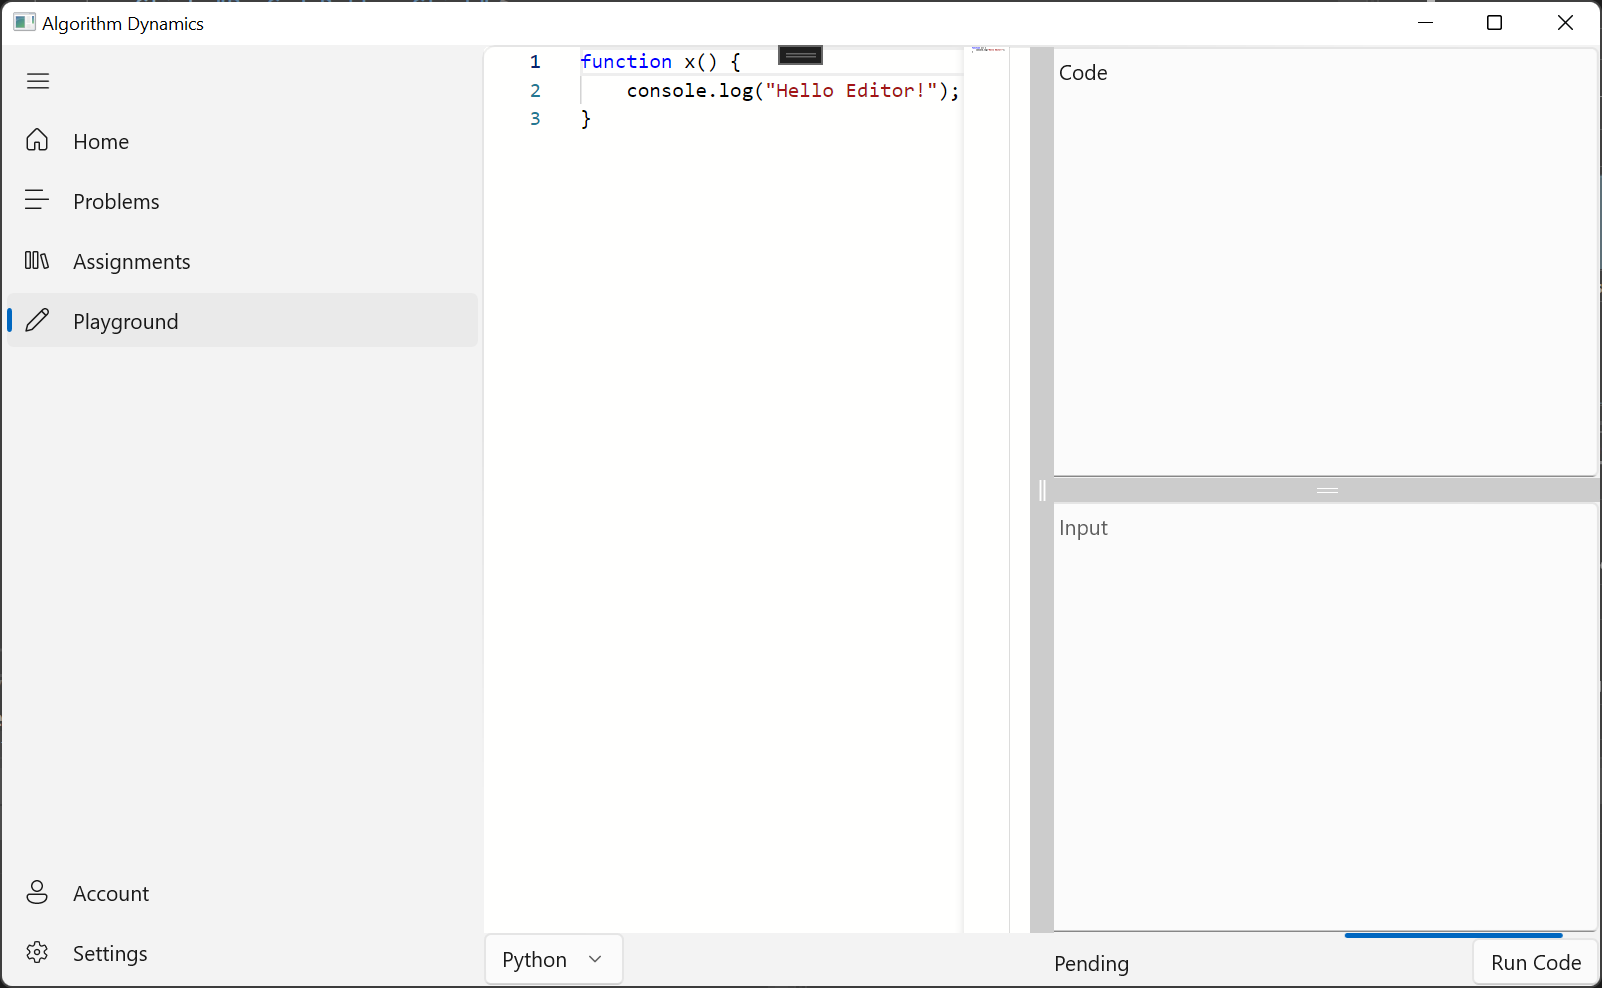
\includegraphics[width=\textwidth, height=\textheight, keepaspectratio]{PlaygroundPage-Layout}

All controls work correctly and they can be resized by the grid splitter. Now I need to interact with the code editer. I need to be able to get the code inside, set its programming language and color theme. To pass the config data to the editor, I will need to serialize the data into a JSON string and send it through web message. To avoid hand crafting the JSON string, I create a new class \code{EditorConfig} and use the \code{System.Text.Json} library to serialize the data.

\begin{minted}{csharp}
public class EditorConfig
{
    public EditorConfig(string theme, string language, string code)
    {
        Theme = theme;
        Language = language;
        Code = code;
    }
    public string? Theme { get; set; } = null;
    public string? Language { get; set; } = null;
    public string? Code { get; set; } = null;
}
\end{minted}

I then create a helper function to send the config data to the editor. It takes in an instance of the EditorConfig and serializes it into a JSON string, then send it through a web message. And for the testing purpose, I send the message when initializing the editor.

\begin{minted}{csharp}
/// <summary>
/// Update the editor config of the Monaco Editor
/// </summary>
/// <param name="editorConfig"></param>
private void UpdateEditorConfig(EditorConfig editorConfig)
{
    WebView.CoreWebView2.PostWebMessageAsJson(JsonSerializer.Serialize(editorConfig));
}


async void InitializeWebViewAsync()
{
    // ...
    UpdateEditorConfig(new EditorConfig("vs-dark", "python", "print(1)"));
}
\end{minted}

On the web end, I need to listen to the web message and process the data received.

\begin{minted}{javascript}
// Receive and set theme/language/code
window.chrome.webview.addEventListener('message', (e) => {
    console.log(e)
    let data = e.data
    if (data.Theme) monaco.editor.setTheme(data.Theme)
    if (data.Language) monaco.editor.setModelLanguage(window.editor.getModel(), data.Language)
    if (data.Code) window.editor.getModel().setValue(data.Code)
})
\end{minted}

Now, when I open the PlaygroundPage, a code editor with dark theme and syntax highlighting for Python should be loaded.

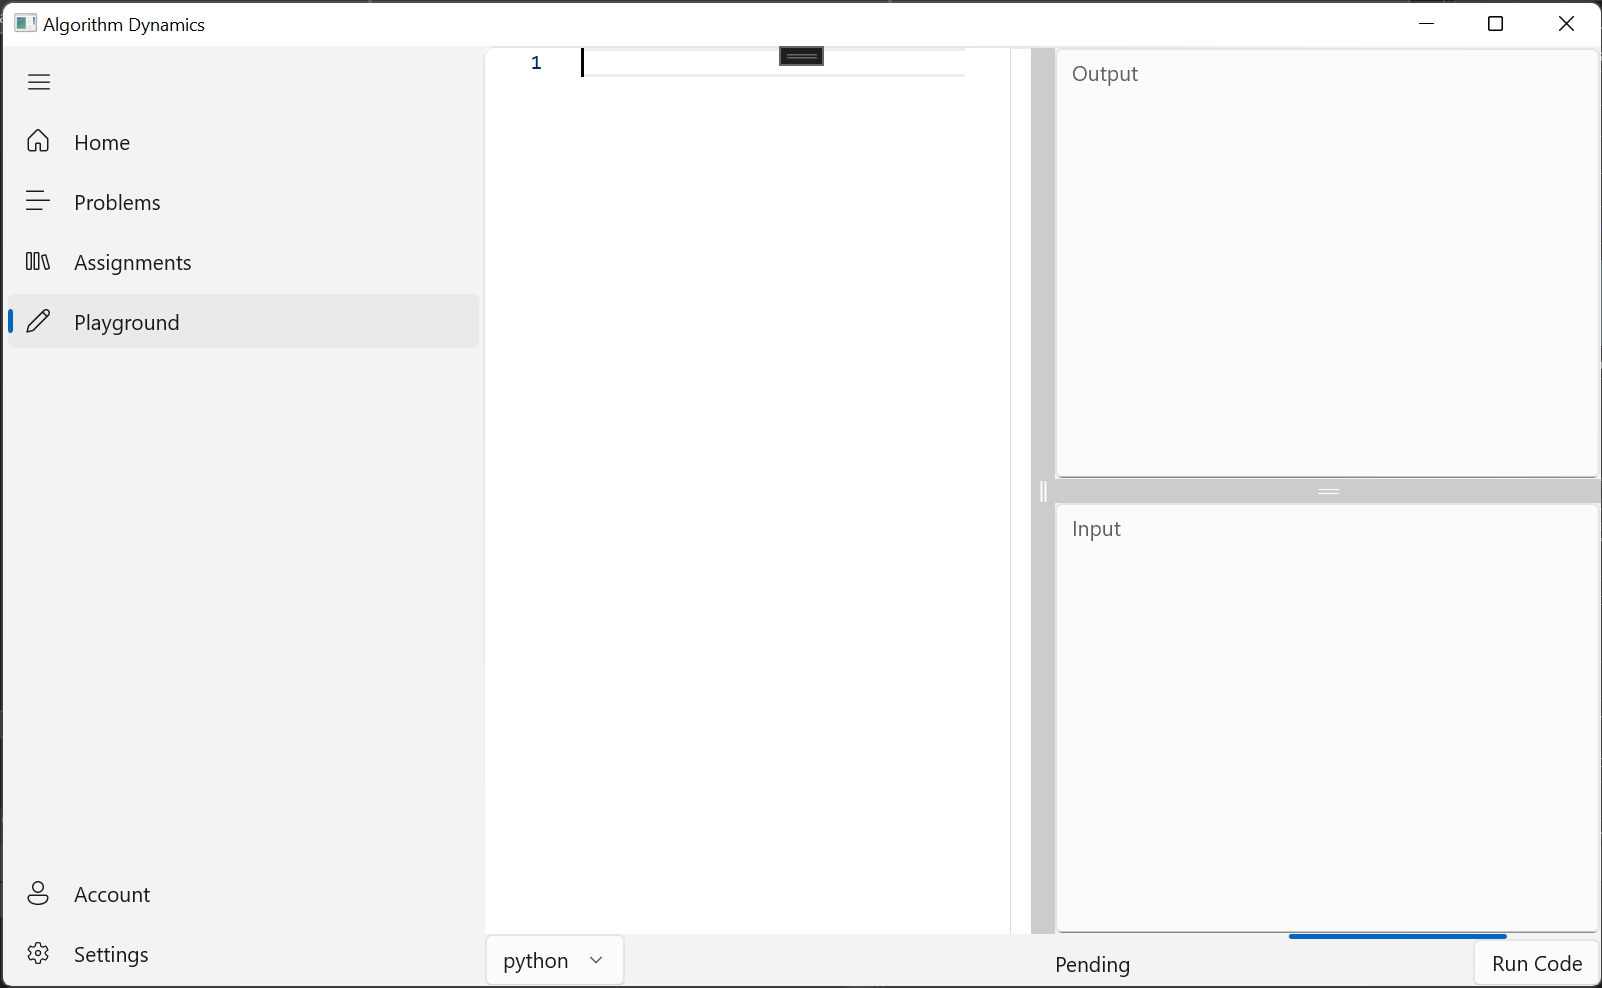
\includegraphics[width=\textwidth, height=\textheight, keepaspectratio]{PlaygroundPage-EditorConfig-NotLoading}

However, it is clearly not loading. Neither the theme, the syntax highlighting nor the code is set. It is clear that the config has not been passed correctly. When I open the devtool, nothing is in the output, which means that \code{console.log(e)} has not been called.

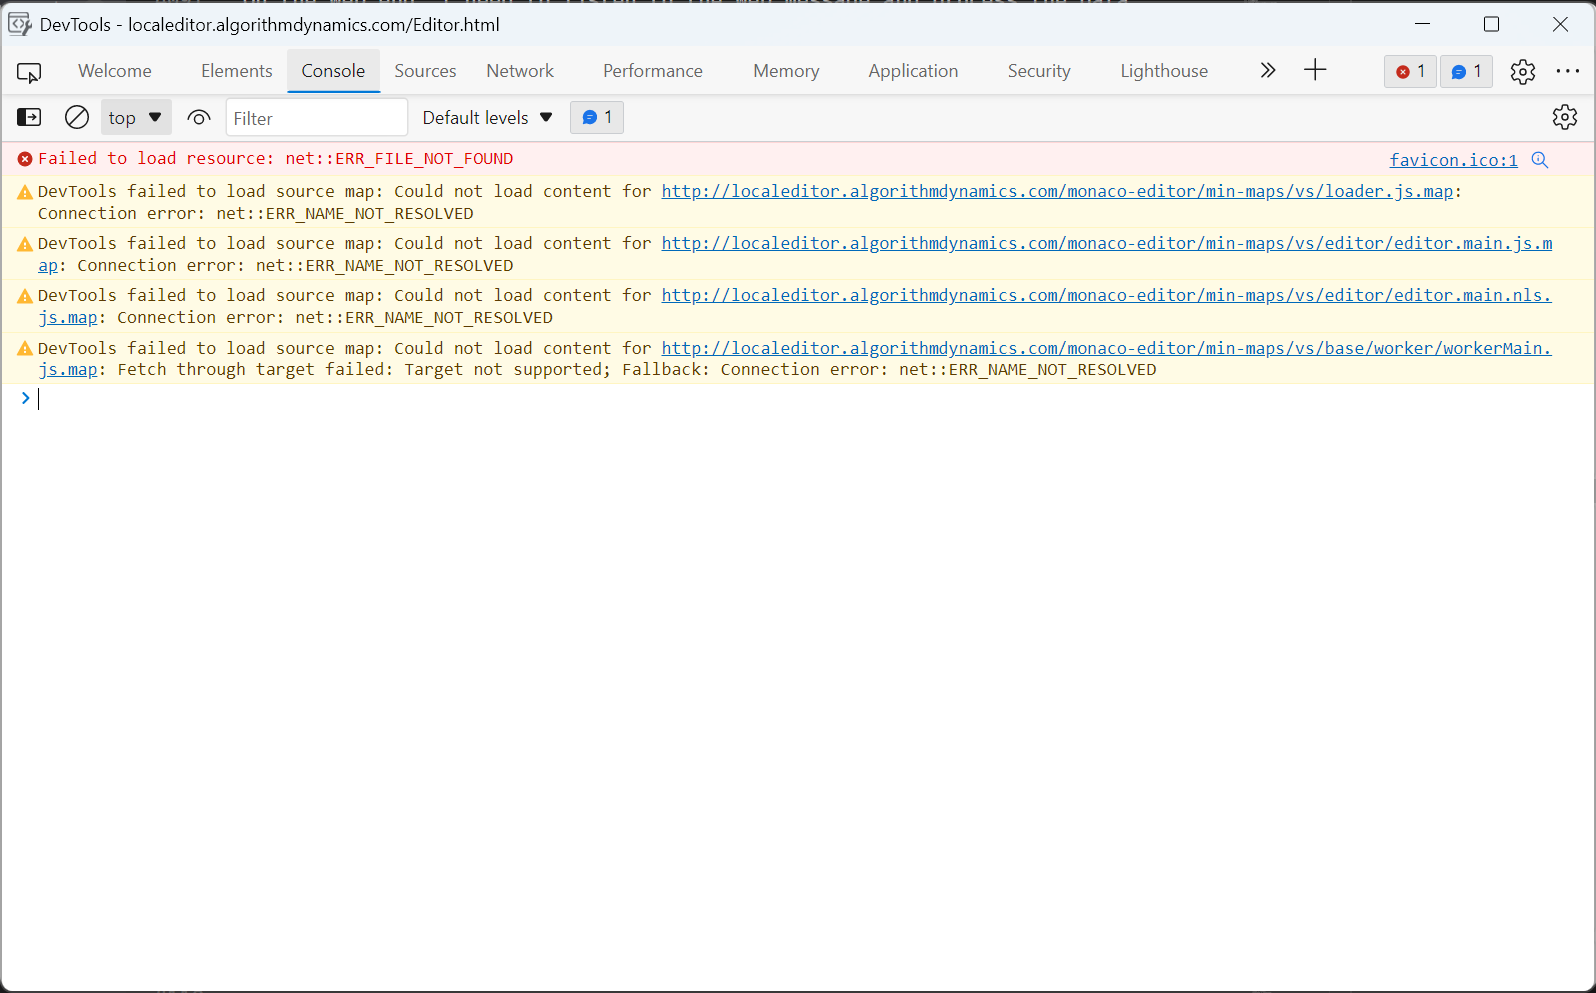
\includegraphics[width=\textwidth, height=\textheight, keepaspectratio]{PlaygroundPage-EditorConfig-NotLoading-Devtool}

I suspect this is caused by the fact that at the time the web message is sent, the Monaco Editor is not fully loaded, therefore it has not started listening for the message. To test my hypothesis, instead of sending a message, I will inject a JavaScript script to pass the value through the global window object.

\begin{minted}{csharp}
async void InitializeWebViewAsync()
{
    // ...
    var editorConfig = new EditorConfig("vs-dark", "python", "print(1)");
    await WebView.ExecuteScriptAsync($"window.config={JsonSerializer.Serialize(editorConfig)}");
}
\end{minted}

And on the web end, I initialize the editor with the config data.

\begin{minted}{javascript}
window.editor = monaco.editor.create(document.getElementById('container'), {
    value: window.config?.Code,
    language: window.config?.Language,
    theme: window.config?.Theme
})
\end{minted}

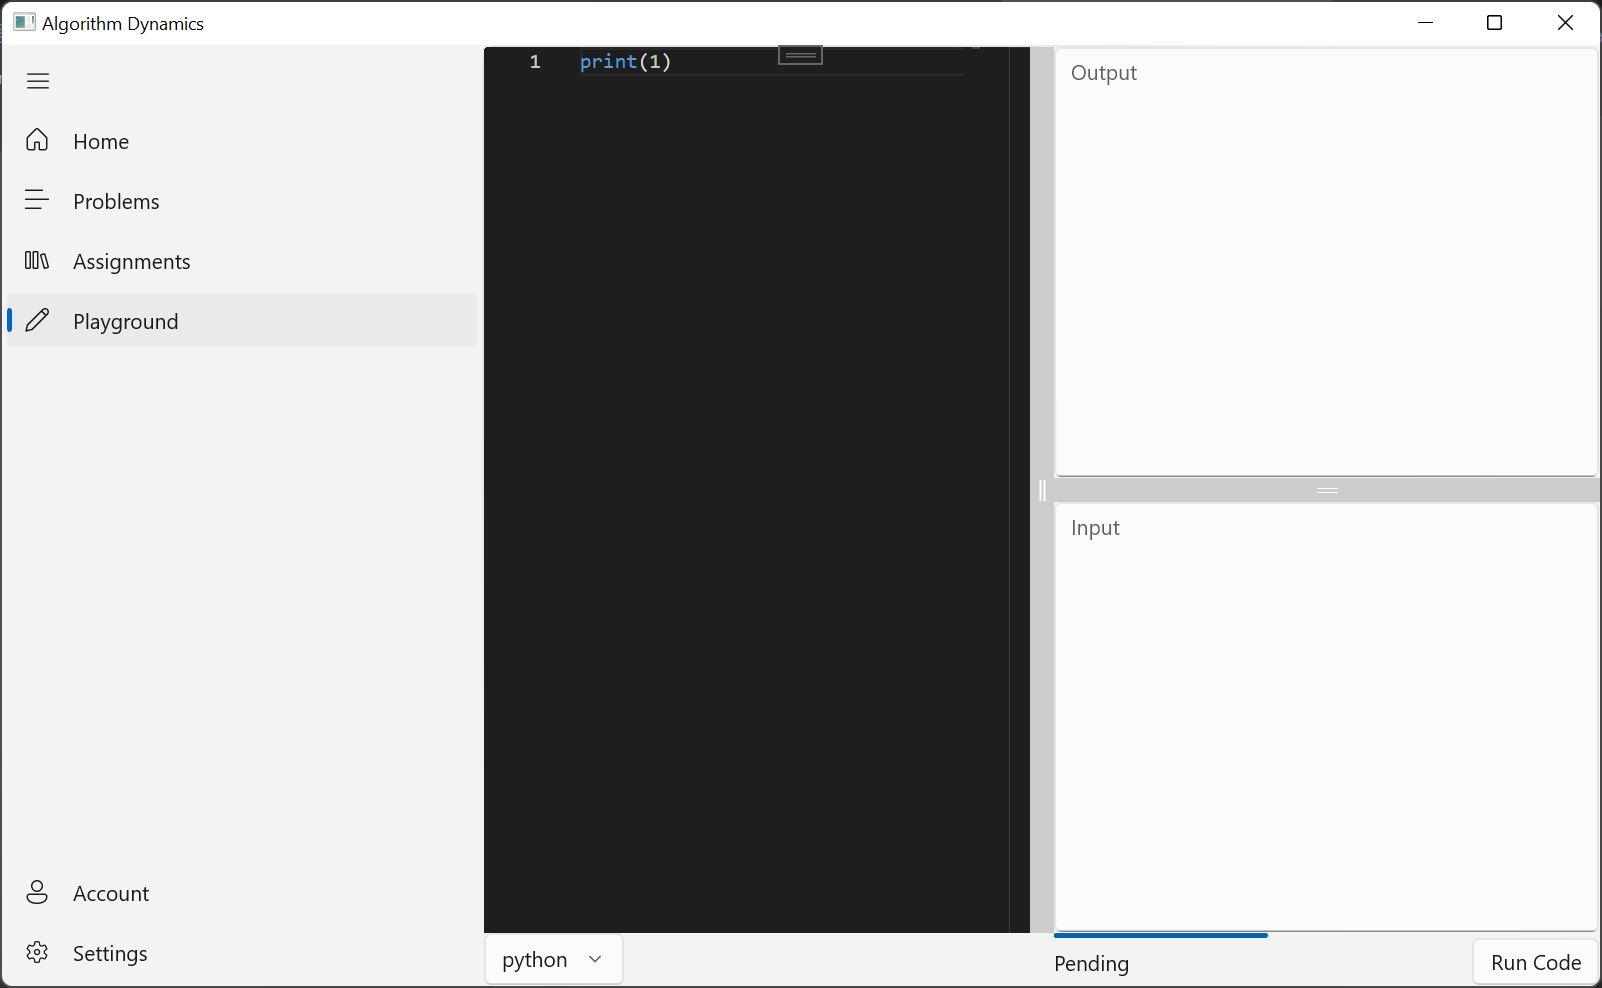
\includegraphics[width=\textwidth, height=\textheight, keepaspectratio]{PlaygroundPage-EditorConfig-Loading}

Now the theme, code, and language config is passed correctly, which also proves my hypothesis is correct. This problem should only occur at the initializing stage. Once the editor is loaded, passing config through web message should work fine.

In order to allow other pages to set the config, I need to expose these three fields by registering them as properties.

\begin{minted}{csharp}
/// <summary>
/// Return the editor theme based on current requested theme
/// </summary>
/// <param name="theme"></param>
/// <returns></returns>
private static string GetTheme(ElementTheme theme)
{
    if (theme == ElementTheme.Dark) return "vs-dark";
    else if (theme == ElementTheme.Light) return "vs";
    return "vs";
}
public string Code
{
    get { return (string)GetValue(CodeProperty); }
    set { SetValue(CodeProperty, value); }
}

public static readonly DependencyProperty CodeProperty =
    DependencyProperty.Register(
        "Code",
        typeof(string),
        typeof(CodeEditor),
        new PropertyMetadata("")
    );

public string Lang
{
    get { return (string)GetValue(LangProperty); }
    set 
    {
        UpdateEditorConfig(new EditorConfig(null, value, null));
        SetValue(LangProperty, value);
    }
}

public static readonly DependencyProperty LangProperty =
    DependencyProperty.Register(
        "Lang",
        typeof(string),
        typeof(CodeEditor),
        new PropertyMetadata("")
    );

public new ElementTheme RequestedTheme
{
    get { return base.RequestedTheme; }
    set
    {
        UpdateEditorConfig(new EditorConfig(GetTheme(value), null, null));
        base.RequestedTheme = value;
    }
}
\end{minted}

Note that \code{UpdateEditorConfig} is called when the language or the requested theme is changed to update the settings. To convert the theme code used in my app into the format of the Monaco Editor, I create a custom helper \code{GetTheme} to do the conversion. And I update the initializing process to use the value from these variables.

\begin{minted}{csharp}
async void InitializeWebViewAsync()
{
    // ...
    var editorConfig = new EditorConfig(GetTheme(RequestedTheme), Lang, Code);
    await WebView.ExecuteScriptAsync($"window.config={JsonSerializer.Serialize(editorConfig)}");
}
\end{minted}

Now, in the PlaygroundPage, I can use the CodeEditor in this way.

\begin{minted}{xml}
<local:CodeEditor
    x:Name="CodeEditor"
    Grid.Row="0"
    Grid.Column="0"
    Grid.RowSpan="2"
    Margin="0 0 8 0"
    Code="hello world!"
    Lang="cpp"
    RequestedTheme="Dark"/>
\end{minted}

Now when I run the app, it should work just like before, but this time with its config exposed and set by the PlaygroundPage. However, I encounter the following exception.

\begin{minted}{text}
System.NullReferenceException
  HResult=0x80004003
  Message=Object reference not set to an instance of an object.
  Source=Algorithm Dynamics
  StackTrace:
   at Algorithm_Dynamics.Controls.CodeEditor.UpdateEditorConfig(EditorConfig editorConfig) in C:\Algorithm-Dynamics\src\Algorithm Dynamics\Controls\CodeEditor.xaml.cs:line 74
\end{minted}

The exception is caused by the \code{UpdateEditorConfig}. And after searching the documentation of the WebView2, the \code{WebView.CoreWebView2} object will be null before it is fully initialized. I can not use the \code{EnsureCoreWebView2Async} method before to ensure it is loaded because it is an async function while \code{UpdateEditorConfig} needs to be called in the setter. So I decide to ignore the null object because it only exists in the initializing stage, and I have passed the config through the global window object anyway.

\begin{minted}{csharp}
private void UpdateEditorConfig(EditorConfig editorConfig)
{
    WebView.CoreWebView2?.PostWebMessageAsJson(JsonSerializer.Serialize(editorConfig));
}
\end{minted}

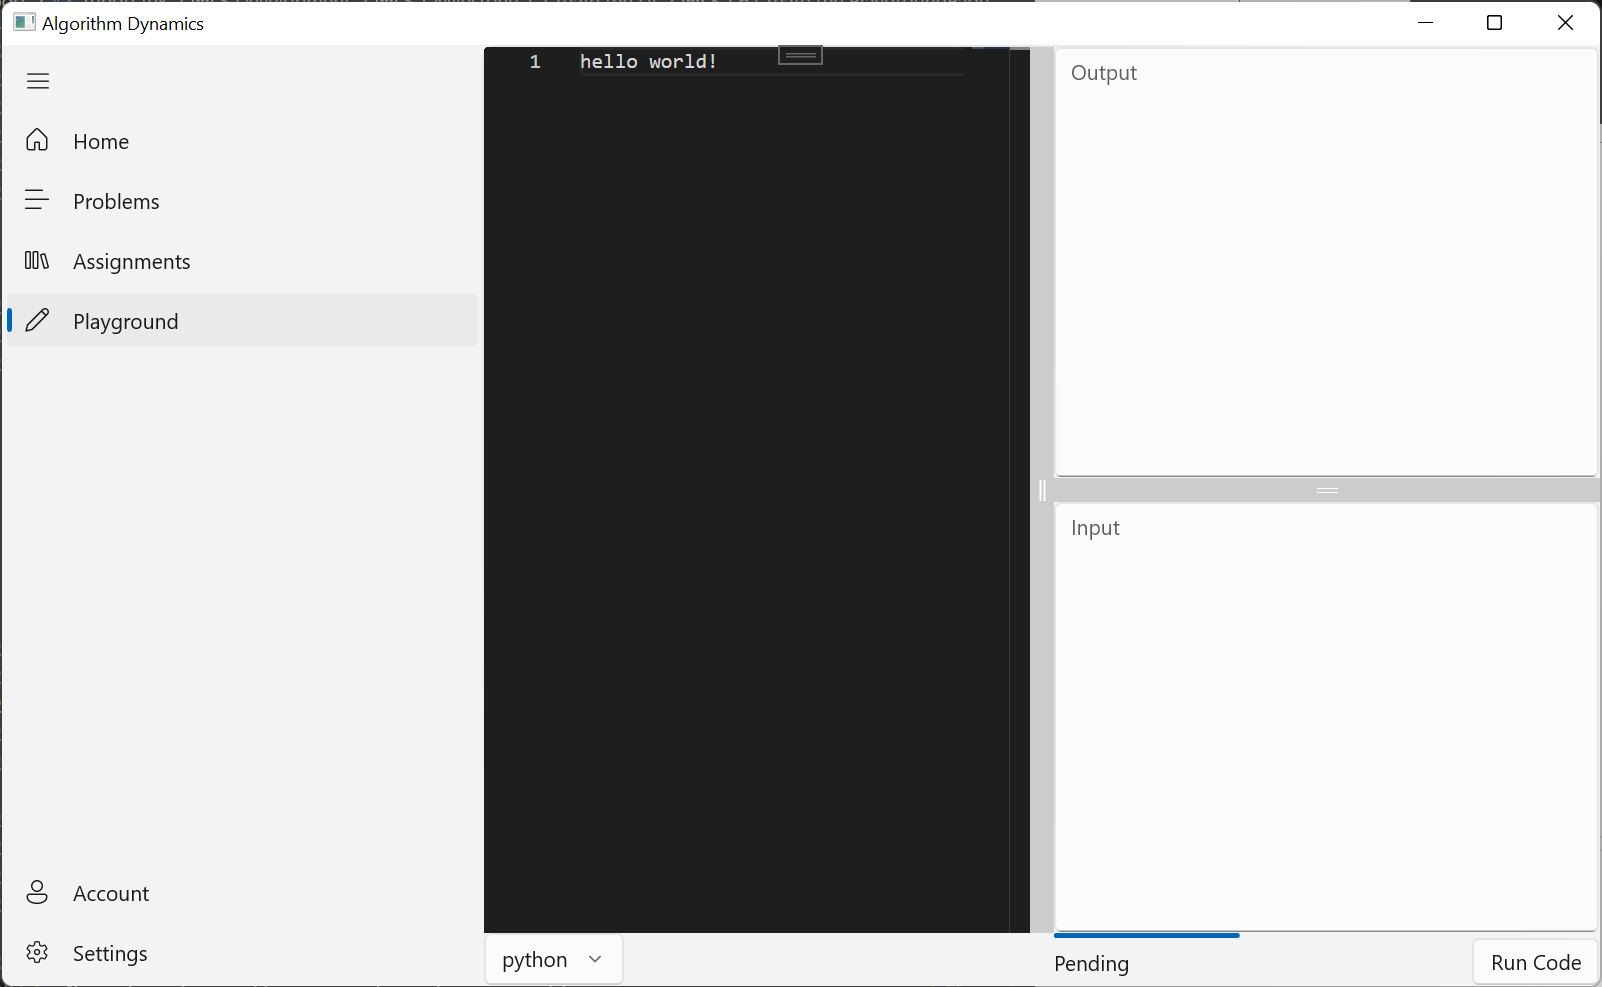
\includegraphics[width=\textwidth, height=\textheight, keepaspectratio]{PlaygroundPage-EditorConfig-Exposed}

Now when I run the app, it works correctly again.

I can pass config to the Monaco Editor now, but I also need to be able to retrieve the code input from the editor. To do this, I add an event listener to the editor, and post a web message when the code is changed.

\begin{minted}{javascript}
// Send code when the code is changed
window.editor.getModel().onDidChangeContent((e) => window.chrome.webview.postMessage(window.editor.getValue()))
\end{minted}

And on the app end, when I receive a new web message, I update the internal Code variable.

\begin{minted}{csharp}
/// <summary>
/// Update the Code when receive the value send by the Monaco Editor
/// </summary>
/// <param name="sender"></param>
/// <param name="args"></param>
private void CoreWebView2_WebMessageReceived(CoreWebView2 sender, CoreWebView2WebMessageReceivedEventArgs args)
{
    string data = args.TryGetWebMessageAsString();
    Code = data;
}

async void InitializeWebViewAsync()
{
    // ...
    WebView.CoreWebView2.WebMessageReceived += CoreWebView2_WebMessageReceived;
    // ...
}
\end{minted}

To test it is working, I bind the output box on the PlaygroundPage to CodeEditor.Code variable. When I type in the code editor, I should see the code in the output box updated with my typing.

\begin{minted}{xml}
<TextBox
    x:Name="OutputBox"
    Grid.Row="0"
    Grid.Column="1"
    Margin="8 0 0 8"
    PlaceholderText="Output"
    IsSpellCheckEnabled="False"
    AcceptsReturn="True"
    Text="{x:Bind CodeEditor.Code, Mode=OneWay}"/>
\end{minted}

When I run the app and start typing in the code editor, the output panel updates as expected, which means I have retrieved the code from the Monaco Editor successfully.

\includegraphics[width=\textwidth, height=\textheight, keepaspectratio]{PlaygroundPage-Editor-CodeSync}

I am not able to implement the full function of the PlaygroundPage right now since the Judger has not been implemented yet. But there is one last thing, I need to make the language ComboBox working. When the user selects a different programming, the syntax highlighting should adjust accordingly. This should be very easy to do since I have already implemented the config updaing function.

I add a new event handler to process the selection change event.

\begin{minted}{xml}
<ComboBox
    x:Name="LanguageComboBox"
    SelectedIndex="0"
    VerticalAlignment="Stretch"
    SelectionChanged="LanguageComboBox_SelectionChanged">
    <x:String>python</x:String>
    <x:String>c</x:String>
    <x:String>cpp</x:String>
    <x:String>javascript</x:String>
</ComboBox>
\end{minted}

And when I update the Lang variable, everything should just work.

\begin{minted}{csharp}
private void LanguageComboBox_SelectionChanged(object sender, SelectionChangedEventArgs e)
{
    CodeEditor.Lang = LanguageComboBox.SelectedItem.ToString();
}
\end{minted}

\includegraphics[width=\textwidth, height=\textheight, keepaspectratio]{PlaygroundPage-Editor-SyntaxHighlighting-Python}

\includegraphics[width=\textwidth, height=\textheight, keepaspectratio]{PlaygroundPage-Editor-SyntaxHighlighting-Cpp}

\includegraphics[width=\textwidth, height=\textheight, keepaspectratio]{PlaygroundPage-Editor-SyntaxHighlighting-JavaScript}

And it turns out to work perfectly as I expected. I can change the syntax highlighting in runtime smoothly.

I have finished the PlaygroundPage in this iteration. I will move on to the CodingPage next, which should be relatively simple because I have encapsulated the code editor into a user control and it can be easily reused.

Just before I plan to start the CodingPage, I find another bug with the Editor control. When the user navigate from the PlaygroundPage to another page, and then navigate back, the editor config cannot be loaded correctly. After some more research, it turns out that the WebView2 component is not destroyed after the page is unloaded, so when the next time it is loaded, it initialize much faster and load before \code{window.config} is set. I decide to design a three-way handshake protocol to solve this problem once and for all.

\includegraphics[width=\linewidth]{webviewHandshake}

At first, the WebView starts loading, and sends a message to request the initial configuration for the Monaco Editor when it is ready. The CodeEditor will keep listening until it receives the request. Then it will send the request and starts listening again. When the Monaco Editor is fully loaded, another message is sent to tell the CodeEditor it is ready. Then the initialization procedure is completed.

\begin{minted}{javascript}
require.config({ paths: { vs: 'monaco-editor/min/vs' } })
require(['vs/editor/editor.main'], () => {
    window.chrome.webview.postMessage('[Status] Request Configuration')
    window.chrome.webview.addEventListener('message', init)
})
function init() {
    // Remove the event listener
    window.chrome.webview.removeEventListener('message', init)
    // Initialize the code editor
    window.editor = monaco.editor.create(document.getElementById('container'), {
        value: window.config.Code,
        language: window.config.Language,
        theme: window.config.Theme
    })
    // Process resize event
    window.addEventListener("resize", () => window.editor.layout())
    // Send code when the code is changed
    window.editor.getModel().onDidChangeContent((e) => 
        window.chrome.webview.postMessage('[Data] ' + window.editor.getValue()))
    // Receive and set theme/language/code
    window.chrome.webview.addEventListener('message', (e) => {
        let data = e.data
        if (data.Theme) monaco.editor.setTheme(data.Theme)
        if (data.Language) monaco.editor.setModelLanguage(window.editor.getModel(), data.Language)
        if (data.Code) window.editor.getModel().setValue(data.Code)
    })
    // Ready
    window.chrome.webview.postMessage('[Status] Ready')
}
\end{minted}

For the CodeEditor control, I add a progress ring to display when it is going through the initilazation process.

\begin{minted}{xml}
<Grid>
    <WebView2 
        x:Name="WebView"
        HorizontalAlignment="Stretch"
        VerticalAlignment="Stretch"
        Visibility="Collapsed"/>
    <ProgressRing
        x:Name="ProgressRing"
        IsActive="True"
        HorizontalAlignment="Center"
        VerticalAlignment="Center"
        Visibility="Visible"/>
</Grid>
\end{minted}

\begin{minted}{csharp}
/// <summary>
/// Process the initialization process
/// Update the Code when receive the value send by the Monaco Editor
/// </summary>
/// <param name="sender"></param>
/// <param name="args"></param>
private async void CoreWebView2_WebMessageReceived(CoreWebView2 sender, CoreWebView2WebMessageReceivedEventArgs args)
{
    string data = args.TryGetWebMessageAsString();
    if (data == "[Status] Request Configuration")
    {
        EditorConfig editorConfig = new (GetTheme(RequestedTheme), Lang, Code);
        await WebView.ExecuteScriptAsync($"window.config={JsonSerializer.Serialize(editorConfig)}");
        WebView.CoreWebView2.PostWebMessageAsString("Configuration Sent");
    }
    else if (data == "[Status] Ready")
    {
        ProgressRing.Visibility = Visibility.Collapsed;
        WebView.Visibility = Visibility.Visible;
    } 
    else
    {
        // [Data] actual code
        Code = data.Substring("[Data] ".Length, data.Length - "[Data] ".Length);
        return;
    }
}
\end{minted}

Now, it is ok to navigate around different pages, and the editor will always be initialized correctly.

After testing the PlaygroundPage for a longer time, I find another issue. The memory usage of the app keep increasing each time when I navigate to and away from the PlaygroundPage. The memory garbage collection does not seem to work as expected. I suspect that is caused by the WebView2 control not being destroyed correctly. To verify my hypothesis, I use the Porcess Explorer \cite{microsoft:docs:process-explorer} to examine the process tree of the app.

\includegraphics[width=\textwidth, height=\textheight, keepaspectratio]{Process-Explorer-WebView2}

As I expected, the WebView2 process is created not destroyed when I navigate away from the PlaygroundPage. And each time a new instance is create, which is causing the memory leak. After some researching on the lifecycle of the WebView2 component \cite{github:microsoft-ui-xaml:4752}, I found that I can call \code{WebView2.Close()} to manually dispose it. So I add a new procedure to handle the control unload event.

\begin{minted}{csharp}
private void CodeEditor_Unloaded(object sender, RoutedEventArgs e)
{
    // Close the WebView when unloaded
    // https://github.com/microsoft/microsoft-ui-xaml/issues/4752
    WebView.Close();
}
\end{minted}

Now, when I navigate away from the PlaygroundPage, I can see from the Process Explorer that all WebView2 processes are killed. And the memory usage fall back to the initial state correctly.

\includegraphics[width=\textwidth, height=\textheight, keepaspectratio]{Process-Explorer-WebView2-Destroyed}

\subsubsection{Testing and validation}

\begin{tabulary}{\linewidth}{|L|l|L|}
    \hline
    Test & Result & Remark \\
    \hline
    Does it load & Pass & \\
    \hline
    Can each section be resized correctly & Pass & \\
    \hline
    Does the CodeEditor work correctly & Pass & \\
    \hline
    Does the language ComboBox work correctly & Pass & \\
    \hline
    Does the input output box work correctly & Pass & \\
    \hline
    Does the Run Code button work & Failed & The Run Code function will be implemented after the Judger is ready. \\
    \hline
    Is the CodeEditor unloaded correctly on close & Pass & \\
    \hline
\end{tabulary}

\subsection{Create the CodingPage}

\subsubsection{Implementation}

I use a grid with 4 rows and 2 columns to organize all elements in the CodingPage.

\begin{minted}{xml}
<Page
    x:Class="Algorithm_Dynamics.Pages.CodingPage"
    xmlns="http://schemas.microsoft.com/winfx/2006/xaml/presentation"
    xmlns:x="http://schemas.microsoft.com/winfx/2006/xaml"
    xmlns:local="using:Algorithm_Dynamics.Controls"
    xmlns:controls="using:CommunityToolkit.WinUI.UI.Controls"
    xmlns:d="http://schemas.microsoft.com/expression/blend/2008"
    xmlns:mc="http://schemas.openxmlformats.org/markup-compatibility/2006"
    mc:Ignorable="d"
    Background="{ThemeResource ApplicationPageBackgroundThemeBrush}">
    <Grid>
        <Grid.RowDefinitions>
            <RowDefinition Height="auto"/>
            <RowDefinition Height="2*"/>
            <RowDefinition Height="*"/>
            <RowDefinition Height="auto"/>
        </Grid.RowDefinitions>

        <Grid.ColumnDefinitions>
            <ColumnDefinition Width="*"/>
            <ColumnDefinition Width="*"/>
        </Grid.ColumnDefinitions>

        <!-- ...  -->
</Page>
\end{minted}

I put a pivot on the top left, which holds two components, the MarkdownTextBlock for the description of the problem and the submission grid. The user can switch between them by clicking the pivot header.

\begin{minted}{xml}
<Pivot
    Grid.Row="0"
    Grid.RowSpan="3"
    Grid.Column="0"
    Margin="0 0 8 0">
    <PivotItem Header="Problem">
        <ScrollViewer
            HorizontalScrollBarVisibility="Disabled"
            VerticalScrollBarVisibility="Auto">
            <controls:MarkdownTextBlock
                x:Name="ProblemMarkdownTextBlock"
                Margin="8"
                Background="{ThemeResource ApplicationPageBackgroundThemeBrush}"
                Text="{x:Bind CodeEditor.Code, Mode=OneWay}"/>
        </ScrollViewer>
    </PivotItem>
    <PivotItem Header="Submissions">
        <controls:DataGrid
            x:Name="SubmissionsDataGrid"
            AutoGenerateColumns="True"
            ItemsSource="{x:Bind Submissions, Mode=OneWay}">
        </controls:DataGrid>
    </PivotItem>
</Pivot>
\end{minted}

I place the language selection box and the fullscreen button on the top right.

\begin{minted}{xml}
<Grid
    Grid.Row="0"
    Grid.Column="1"
    Margin="8">
    <Grid.ColumnDefinitions>
        <ColumnDefinition Width="*"/>
        <ColumnDefinition Width="*"/>
    </Grid.ColumnDefinitions>
    <ComboBox
        Grid.Column="0"
        x:Name="LanguageComboBox"
        SelectedIndex="0"
        VerticalAlignment="Stretch"
        SelectionChanged="LanguageComboBox_SelectionChanged">
        <x:String>python</x:String>
        <x:String>c</x:String>
        <x:String>cpp</x:String>
        <x:String>javascript</x:String>
    </ComboBox>
    <Button
        x:Name="FullScreenButton"
        Grid.Column="1"
        HorizontalAlignment="Right"
        Click="FullScreenButton_Click"
        ToolTipService.ToolTip="Fullscreen (F11)">
        <FontIcon
            x:Name="FullScreenIcon"
            FontFamily="Segoe Fluent Icons"
            Glyph="&#xE740;"/>
        <Button.KeyboardAccelerators>
            <KeyboardAccelerator Key="F11"/>
        </Button.KeyboardAccelerators>
    </Button>
</Grid>
\end{minted}

On the button right, I place the code editor and  Input/Output/Error panel inside another pivot so the user can navigate between them. Because the code editor has been encapsulated as a user control before, I can easily import it here.

\begin{minted}{xml}
<local:CodeEditor
    x:Name="CodeEditor"
    Grid.Column="1"
    Grid.Row="1"
    Margin="8 0 0 8"/>
<Pivot
    Grid.Row="2"
    Grid.Column="1"
    Margin="8 8 0 0">
    <PivotItem Header="Input">
        <TextBox
            x:Name="InputTextBox"
            x:FieldModifier="public"
            PlaceholderText="Input Panel"
            AcceptsReturn="True"/>
    </PivotItem>
    <PivotItem Header="Output">
        <TextBox
            x:Name="OutputTextBox"
            x:FieldModifier="public"
            PlaceholderText="Output Panel"
            AcceptsReturn="True"/>
    </PivotItem>
    <PivotItem Header="Error">
        <TextBox
            x:Name="ErrorTextBox"
            x:FieldModifier="public"
            PlaceholderText="Error Panel"
            AcceptsReturn="True"/>
    </PivotItem>
</Pivot>
\end{minted}

At the bottom, I place the problem navigation buttons, the status text block, a progress bar and the run code and submission button.

\begin{minted}{xml}
<Grid
    Grid.Row="3"
    Grid.Column="1">
    <Grid.RowDefinitions>
        <RowDefinition Height="auto"/>
        <RowDefinition Height="*"/>
    </Grid.RowDefinitions>
    
    <Grid.ColumnDefinitions>
        <ColumnDefinition Width="*"/>
        <ColumnDefinition Width="auto"/>
        <ColumnDefinition Width="auto"/>
    </Grid.ColumnDefinitions>

    <ProgressBar
        Grid.Row="0"
        Grid.Column="0"
        Grid.ColumnSpan="3"
        IsIndeterminate="True"
        ShowPaused="False"
        ShowError="False"/>
    <TextBlock
        Grid.Row="1"
        Grid.Column="0"
        Text="Status"
        VerticalAlignment="Center"/>
    <Button
        Grid.Row="1"
        Grid.Column="2"
        x:Name="SubmitCodeButton"
        Content="Submit"
        Style="{StaticResource AccentButtonStyle}"/>
    <Button
        Grid.Row="1"
        Grid.Column="1"
        Content="Run Code"/>
</Grid>

<Grid
    Grid.Row="3"
    Grid.Column="0">
    <Grid.ColumnDefinitions>
        <ColumnDefinition Width="auto"/>
        <ColumnDefinition Width="auto"/>
        <ColumnDefinition Width="auto"/>
    </Grid.ColumnDefinitions>
    <Button
        Grid.Column="0"
        VerticalAlignment="Stretch">
        <Button.Content>
            <FontIcon FontFamily="Segoe Fluent Icons" Glyph="&#xE76B;"/>
        </Button.Content>
    </Button>
    <DropDownButton
        Grid.Column="1"
        Content="Problem 0"
        VerticalAlignment="Stretch">
        <DropDownButton.Flyout>
            <MenuFlyout Placement="Top">
                <MenuFlyoutItem Text="Problem 1"/>
                <MenuFlyoutItem Text="Problem 2"/>
                <MenuFlyoutItem Text="Problem 3"/>
            </MenuFlyout>
        </DropDownButton.Flyout>

    </DropDownButton>
    <Button
        Grid.Column="2"
        VerticalAlignment="Stretch">
        <Button.Content>
            <FontIcon FontFamily="Segoe Fluent Icons" Glyph="&#xE76C;"/>
        </Button.Content>
    </Button>
</Grid>
\end{minted}

At the end, I add two grid splitters between the problem panel and the editor, the editor and the panel so users can resize each window to fit their needs.

When I build and run the app, I encounter a problem - I cannot navigate to the CodingPage. Unlike the previous pages, the CodingPage is not a top-level page, it is opened when the user select a problem or an assignment. So I need to link the start problem button to the CodingPage. So for the Start button on the ProblemsPage, I add a StartProblem function to handle the click event.

\begin{minted}{xml}
<Button
    Content="Start"
    Grid.Column="4"
    HorizontalAlignment="Stretch"
    Margin="12 0 0 0"
    Click="StartProblem"/>
\end{minted}

\begin{minted}{csharp}
/// <summary>
/// Navigate to the CodingPage, pass the current Problem and ProblemList
/// </summary>
/// <param name="sender"></param>
/// <param name="e"></param>
private void StartProblem(object sender, RoutedEventArgs e)
{
    App app = (App)Application.Current;
    // TODO pass the selected problem to the CodingPage
    app.ContentFrame.Navigate(typeof(CodingPage));
    app.MainNavView.SelectedItem = null;
}
\end{minted}

The function should also pass the selected problem and the problem list through the Navigate function. But since the data structure is not implemented, for now, it just navigates to the page without passing any data.

Now when I run the app, I can navigate to the CodingPage through the ProblemsPage and see all the layout I defined before.

\includegraphics[width=\textwidth, height=\textheight, keepaspectratio]{CodingPage-Layout}

When I provide the screenshot to my stakeholder PCloud, he says that the controls are quite ugly, especially the pivot and the grid splitter, the font and color theme does not seem to match the overall design. I agree with him, so I decide to add some style to the pivot and the grid splitter.

I create a new file Generic.xaml to store all the styles. In App.xaml, I import the Generic.xaml file.

\begin{minted}{xml}
<Application.Resources>
    <ResourceDictionary>
        <ResourceDictionary.MergedDictionaries>
            <XamlControlsResources xmlns="using:Microsoft.UI.Xaml.Controls" />
            <ResourceDictionary Source="/Themes/Generic.xaml"/>
            <!-- Other merged dictionaries here -->
        </ResourceDictionary.MergedDictionaries>
        <!-- Other app resources here -->
    </ResourceDictionary>
</Application.Resources>
\end{minted}

For the GridSplitter, I reference the design in DevToys\cite{github:DevToys:Generic.xaml} by setting the background color to transparent which makes the GridSplitter less significant.

For the Pivot, I reference the design from the Windows Calculator\cite{github:calculator:Calculator.xaml}, which modifies the Pivot to make it look like the modern NavigationView.

\includegraphics[width=\textwidth, height=\textheight, keepaspectratio]{CodingPage-Theme}

After applying the custom theme, the interface looks much more modern and consistent.

Next I will implement the full screen button. It will be a toggle, when clicking in the window mode, it set the window to full screen. When clicking in the full screen mode, it sets the window back to a window. I also assigned a keyboard accelerator F11 to the button, so the user can toggle it by keyboard.

\begin{minted}{xml}
<Button
    x:Name="FullScreenButton"
    Grid.Column="1"
    HorizontalAlignment="Right"
    Click="FullScreenButton_Click"
    ToolTipService.ToolTip="Fullscreen (F11)">
    <FontIcon
        x:Name="FullScreenIcon"
        FontFamily="Segoe Fluent Icons"
        Glyph="&#xE740;"/>
    <Button.KeyboardAccelerators>
        <KeyboardAccelerator Key="F11"/>
    </Button.KeyboardAccelerators>
</Button>
\end{minted}

In the \code{FullScreenButton_Click} function, I implement the logic of the toggle button. It sets the \code{AppWindowPresent} property\cite{microsoft:docs:windowing-overview} to the opposite value and assign the correct icon\cite{microsoft:docs:segoe-fluent-icons-font}.

\begin{minted}{csharp}
/// <summary>
/// Toggle the fullscreen mode for the app
/// Toggle the <see cref="AppWindowPresenterKind"/> and <see cref="FullScreenIcon.Glyph"/>
/// </summary>
/// <param name="sender"></param>
/// <param name="e"></param>
private void FullScreenButton_Click(object sender, RoutedEventArgs e)
{
    AppWindow window = MainWindow.AppWindow;
    if (window.Presenter.Kind == AppWindowPresenterKind.Overlapped)
    {
        window.SetPresenter(AppWindowPresenterKind.FullScreen);
        FullScreenIcon.Glyph = "\xE73F";
    }
    else
    {
        window.SetPresenter(AppWindowPresenterKind.Overlapped);
        FullScreenIcon.Glyph = "\xE740";
    }
}
\end{minted}

Now when I click the button, it does go into the fullscreen mode with the correct button icon set. But I notice that the system taskbar is blank instead of filled with the app window. After doing some research, it turns out that this is caused by an internal bug of the WindowsAppSDK\cite{github:WindowsAppSDK:1853} and I cannot fix it on my side. I will just leave it like this until a new version of the SDK is released.

\includegraphics[width=\textwidth, height=\textheight, keepaspectratio]{CodingPage-FullScreen-Bug.png}

For the other parts, the submission records depend on the database, and the run code and submit function depends on the Judger, so in this iteration, I will leave the page like this.

\subsubsection{Testing and validation}

\begin{tabulary}{\linewidth}{|L|l|L|}
    \hline
    Test & Result & Remark \\
    \hline
    Does it load & Failed & This feature is not fully implemented. When the CodingPage loads, it should take in two parameter, the current problem and a problem list for navigation. The main page can load correctly, but the support for these two parameters are not yet implemented because the data structure is not implemented yet. \\
    \hline
    Does the full screen button work & Pass & \\
    \hline
    Does the markdown text block work & Pass & \\
    \hline
    Does the code editor work & Pass & \\
    \hline
    Does the input panel work & Pass & \\
    \hline
    Does the output panel work & Pass & \\
    \hline
    Does the error panel work & Pass & \\
    \hline
    Does the language selection box work & Pass & \\
    \hline
    Does the Run Code button work & Failed & Not implemented because the Judger is not ready. \\
    \hline
    Does the Submit button work & Failed & Not implemented because the Judger is not ready. \\
    \hline
    Does the Submit problem navigation & Failed & Not implemented because the data structure is not ready. \\
    \hline
    Does the submission history table work & Failed & Not implemented because the database is not ready. \\
    \hline
\end{tabulary}

\subsection{Create the AccountPage}

\subsubsection{Implementation}

For the AccountPage, I use a grid of two row to divide the two sections for the account information and the statistics data. For the account information, I decide to use the RelativePanel to construct the layout to make it responsive to different sizes of the window. For the statistics data, I use the AdaptiveGridView which is used for the HomePage as well, so the data can be dynamically added in the code behind and make it a lot easier to add custom statistics later.

\begin{minted}{xml}
<Grid>
    <Grid.RowDefinitions>
        <RowDefinition Height="*"/>
        <RowDefinition Height="*"/>
    </Grid.RowDefinitions>

    <RelativePanel
        Grid.Row="0"
        HorizontalAlignment="Stretch"
        VerticalAlignment="Stretch">
        <PersonPicture
            x:Name="AvatarPicture"
            Margin="32"
            RelativePanel.AlignLeftWithPanel="True"
            RelativePanel.AlignVerticalCenterWithPanel="True"
            ProfilePicture="https://docs.microsoft.com/windows/uwp/contacts-and-calendar/images/shoulder-tap-static-payload.png" />
        <StackPanel
            RelativePanel.RightOf="AvatarPicture"
            RelativePanel.AlignVerticalCenterWithPanel="True">
            <TextBlock
                Margin="2"
                Text="Name"
                Style="{ThemeResource SubtitleTextBlockStyle}"/>
            <TextBlock
                Margin="2"
                Text="Email"
                Style="{ThemeResource BodyTextBlockStyle}"/>
            <TextBlock
                Margin="2"
                Text="Role"
                Style="{ThemeResource BodyTextBlockStyle}"/>
        </StackPanel>
        <StackPanel
            Margin="32"
            RelativePanel.AlignRightWithPanel="True"
            RelativePanel.AlignVerticalCenterWithPanel="True">
            <Button
                Margin="2"
                HorizontalAlignment="Stretch"
                Content="Edit"/>
            <Button
                Margin="2"
                HorizontalAlignment="Stretch"
                Content="Login"/>
        </StackPanel>
    </RelativePanel>

    <controls:AdaptiveGridView
        x:Name="StatsGridView"
        Grid.Row="1"
        Margin="0"
        ItemsSource="{x:Bind StatsItems}"
        StretchContentForSingleRow="False"
        OneRowModeEnabled="False"
        ItemHeight="120"
        DesiredWidth="240"
        SelectionMode="None"
        IsItemClickEnabled="False"
        Background="{ThemeResource AcrylicBackgroundFillColorDefaultBrush}">
        <GridView.ItemTemplate>
            <DataTemplate x:DataType="models:StatisticsItem">
                <Grid HorizontalAlignment="Stretch">
                    <StackPanel 
                        VerticalAlignment="Center"
                        HorizontalAlignment="Center"
                        Orientation="Vertical"
                        Margin="8">
                        <TextBlock
                            Text="{x:Bind Title}"
                            Margin="2"
                            Style="{ThemeResource BodyStrongTextBlockStyle}"
                            HorizontalAlignment="Center"/>
                        <TextBlock 
                            Text="{x:Bind Data}"
                            Margin="2"
                            HorizontalAlignment="Center"/>
                    </StackPanel>
                </Grid>
            </DataTemplate>
        </GridView.ItemTemplate>
    </controls:AdaptiveGridView>

</Grid>
\end{minted}

Similar to the HomePage, I create a model \code{StatisticsItem} for the statistics data and binds it to the grid. For now, I just add some sample data in for display purpose.

\begin{minted}{csharp}
public class StatisticsItem
{
    public StatisticsItem(string title, string data)
    {
        Title = title;
        Data = data;
    }

    public string Title { get; set; }
    public string Data { get; set; }
}
\end{minted}

\begin{minted}{csharp}
public AccountPage()
{
    InitializeComponent();
    StatsItems.Add(new StatisticsItem("Problem Solved", "10"));
    StatsItems.Add(new StatisticsItem("Problem Attempted", "3"));
    StatsItems.Add(new StatisticsItem("Problem Unsolved", "1100"));
    StatsItems.Add(new StatisticsItem("Correct Rate", "10%"));
    StatsItems.Add(new StatisticsItem("Favourite Topic", "Data structure"));
    StatsItems.Add(new StatisticsItem("Favourite Language", "Python"));
}
public ObservableCollection<StatisticsItem> StatsItems { get; } = new ObservableCollection<StatisticsItem>();
\end{minted}

\includegraphics[width=\textwidth, height=\textheight, keepaspectratio]{AccountPage-Layout}

Next, I want to implement the edit function, which allows the user to change their user name, email address and role. To achieve this, I decide to replace the TextBlocks with TextBoxes for the user to edit the data when the Edit button is clicked. This can be achieved by setting the visibility of the controls. Instead of directly setting the visibility, I decide to bind the visibility property to a public variable named \code{IsEditMode} to determine whether it should display. In order to notify the binded control, I implement the \code{PropertyChanged} event\cite{microsoft:docs:data-binding-in-depth}.

\begin{minted}{csharp}
/// <summary>
/// Invoke when the property is changed.
/// </summary>
public event PropertyChangedEventHandler PropertyChanged = delegate { };

/// <summary>
/// Invoke a new <see cref="PropertyChanged"/> event.
/// </summary>
/// <param name="propertyName">Use <see cref="nameof"/> to get the name of the property.</param>
public void OnPropertyChanged([CallerMemberName] string propertyName = null)
{
    // Raise the PropertyChanged event, passing the name of the property whose value has changed.
    PropertyChanged?.Invoke(this, new PropertyChangedEventArgs(propertyName));
}
\end{minted}

I create a private variable \code{_isEditMode} to record the current state. A public variable \code{IsEditMode} to encapsulated the private variable so I can call the \code{OnPropertyChanged} function I just implemented in the setter. I also create the \code{IsNotEditMode} attribute to handle the boolean inversion.

\begin{minted}{csharp}
private bool _isEditMode = false;
public bool IsEditMode
{
    get => _isEditMode;
    set
    {
        _isEditMode = value;
        OnPropertyChanged(nameof(IsEditMode));
        OnPropertyChanged(nameof(IsNotEditMode));
    }
}
public bool IsNotEditMode
{
    get => !_isEditMode;
}
\end{minted}

Finally, I edit the XAML markup to add the TextBoxes and add the bindings.


\begin{minted}{xml}
<StackPanel
    RelativePanel.RightOf="AvatarPicture"
    RelativePanel.AlignVerticalCenterWithPanel="True">
    <TextBlock
        x:Name="NameTextBlock"
        Margin="2"
        Text="{x:Bind EditNameTextBox.Text, Mode=OneWay}"
        Visibility="{x:Bind IsNotEditMode, Mode=OneWay"
        Style="{ThemeResource SubtitleTextBlockStyle}"/>
    <TextBox
        x:Name="EditNameTextBox"
        PlaceholderText="Name"
        Margin="2"
        Text="Name"
        HorizontalAlignment="Stretch"
        Visibility="{x:Bind IsEditMode, Mode=OneWay"/>
    <TextBlock
        x:Name="EmailTextBlock"
        Margin="2"
        Text="{x:Bind EditEmailTextBox.Text, Mode=OneWay}"
        Visibility="{x:Bind IsNotEditMode, Mode=OneWay"
        Style="{ThemeResource BodyTextBlockStyle}"/>
    <TextBox
        x:Name="EditEmailTextBox"
        PlaceholderText="Email"
        Text="Email"
        Margin="2"
        HorizontalAlignment="Stretch"
        Visibility="{x:Bind IsEditMode, Mode=OneWay"/>
    <TextBlock
        x:Name="RoleTextBlock"
        Margin="2"
        Text="{x:Bind EditRoleComboBox.SelectedValue, Mode=OneWay}"
        Visibility="{x:Bind IsNotEditMode, Mode=OneWay"
        Style="{ThemeResource BodyTextBlockStyle}"/>
    <ComboBox
        x:Name="EditRoleComboBox"
        Visibility="{x:Bind IsEditMode, Mode=OneWay"
        HorizontalAlignment="Stretch"
        Margin="2"
        SelectedIndex="0">
        <x:String>Student</x:String>
        <x:String>Teacher</x:String>
    </ComboBox>
</StackPanel>
\end{minted}

Now when I run the program, I can edit all fields successfully after clicking the Edit button. All the changes are preserved after clicking the Done button.

\includegraphics[width=\textwidth, height=\textheight, keepaspectratio]{AccountPage-Edit}

\includegraphics[width=\textwidth, height=\textheight, keepaspectratio]{AccountPage-Saved}

\subsubsection{Testing and validation}

\begin{tabulary}{\linewidth}{|L|l|L|}
    \hline
    Test & Result & Remark \\
    \hline
    Does it load & Pass & \\
    \hline
    Does the Edit button work & Pass & Note that the changes are not actually saved to the disk, since the settings module will not be implemented in this iteration. \\
    \hline
    Does the login button work & Failed & The login button depends on the API module, which will not be implemented in this iteration. \\
    \hline
    Does the statistics data show up correctly & Pass & Note that the actual data depends on the database module, which is not implemented yet. \\
    \hline
\end{tabulary}

\subsection{Create the CreatePage}

\subsubsection{Implementation}

For the CreateNewProblemPage, it contains a form for the user to input data to create new problems. I use a ScrollViewer to wrap everything up so the user can scroll in the page when the elements overflow. Inside the ScrollViewer, I place a StackPanel as the root panel to organize everything.

\begin{minted}{xml}
<ScrollViewer x:Name="scrollViewer">
    <StackPanel
        Margin="32"
        x:Name="FormStackPanel">
        <!-- Form controls -->
    </StackPanel>
</ScrollViewer>
\end{minted}

I use TextBoxes to allow the user to input problem name, a TokenizingTextBox for the tag, ComboBox for difficult, and NumberBox for time limit and memory limit.

\begin{minted}{xml}
<TextBlock
    Text="Create Problem"
    Style="{ThemeResource TitleTextBlockStyle}"/>
<TextBox
    Margin="0 22 0 0"
    Header="Problem Name"
    MaxLength="64"
    Width="400"
    HorizontalAlignment="Left"/>
<controls:TokenizingTextBox
    Header="Tags"
    Margin="0 22 0 0" 
    Width="400"
    MaximumTokens="3"
    PlaceholderText="Add Tags"
    SelectionMode="Extended"
    HorizontalAlignment="Left"/>
<ComboBox
    Header="Difficulty"
    SelectedIndex="0"
    Margin="0 22 0 0"
    Width="400"
    HorizontalAlignment="Left">
    <x:String>Easy</x:String>
    <x:String>Medium</x:String>
    <x:String>Hard</x:String>
</ComboBox>
<NumberBox
    Header="Time Limit (ms)"
    Value="1000"
    Width="400"
    Minimum="100"
    Margin="0 22 0 0"
    HorizontalAlignment="Left"
    SpinButtonPlacementMode="Inline"
    SmallChange="100"
    LargeChange="500"/>
<NumberBox
    Header="Memory Limit (MB)"
    Value="64"
    Width="400"
    Margin="0 22 0 0"
    Minimum="16"
    HorizontalAlignment="Left"
    SpinButtonPlacementMode="Inline"
    SmallChange="64"
    LargeChange="256"/>
\end{minted}

For the description, I use a Pivot to organize the input TextBox and the preview MarkdownRenderer.

\begin{minted}{xml}
<Pivot
    x:Name="DescriptionPivot">
    <PivotItem
        Header="Description">
        <TextBox
            x:Name="DescriptionTextBox"
            HorizontalAlignment="Stretch"
            VerticalAlignment="Stretch"
            TextWrapping="Wrap" 
            AcceptsReturn="True" 
            IsSpellCheckEnabled="True"
            MinHeight="200"
            MaxHeight="840"/>
    </PivotItem>
    <PivotItem
        Header="Preview">
        <controls:MarkdownTextBlock
            x:Name="ProblemMarkdownTextBlock"
            Margin="8"
            Background="{ThemeResource ApplicationPageBackgroundThemeBrush}"
            Text="{x:Bind DescriptionTextBox.Text, Mode=OneWay}"/>
    </PivotItem>
</Pivot>
\end{minted}

Next, I implement the TestCase list. Similarly as the ProblemList before, I use a ListView and bind the TestCases collection to it.

\begin{minted}{xml}
<ListView
    x:Name="TestCasesListView"
    Margin="0 22 0 0"
    Header="Test Cases"
    SelectionMode="None"
    ItemsSource="{x:Bind TestCases, Mode=OneWay}">
    <ListView.ItemTemplate>
        <DataTemplate x:DataType="local:TestCase">
            <Grid
                Margin="0 10 0 0">
                <Grid.ColumnDefinitions>
                    <ColumnDefinition Width="*"/>
                    <ColumnDefinition Width="*"/>
                    <ColumnDefinition Width="auto"/>
                    <ColumnDefinition Width="auto"/>
                </Grid.ColumnDefinitions>
                <TextBox
                    Grid.Column="0"
                    Margin="4"
                    AcceptsReturn="True"
                    MaxHeight="100"
                    VerticalAlignment="Center"
                    PlaceholderText="Input Data"
                    Text="{x:Bind Input, Mode=TwoWay}"/>
                <TextBox
                    Grid.Column="1"
                    Margin="4"
                    AcceptsReturn="True"
                    MaxHeight="100"
                    VerticalAlignment="Center"
                    PlaceholderText="Output Data"
                    Text="{x:Bind Output, Mode=TwoWay}"/>
                <CheckBox
                    Grid.Column="2"
                    Margin="40 0 0 0"
                    Content="Example"
                    HorizontalAlignment="Center"
                    VerticalAlignment="Center"
                    IsChecked="{x:Bind IsExample, Mode=TwoWay}"/>
                <Button
                    x:Name="DeleteSingleTestCaseButton"
                    Grid.Column="3"
                    Margin="0"
                    VerticalAlignment="Center"
                    HorizontalAlignment="Center"
                    Click="DeleteSingleTestCase">
                    <Button.Content>
                        <SymbolIcon Symbol="Delete"/>
                    </Button.Content>
                </Button>
            </Grid>
        </DataTemplate>
    </ListView.ItemTemplate>
</ListView>
\end{minted}

\begin{minted}{csharp}
public ObservableCollection<TestCase> TestCases = new() { new TestCase("", "", true) };
\end{minted}


I implement a simple TestCase class for this iteration, so the UI can be tested. A more detailed one will be implemented in the later iteration.

\begin{minted}{csharp}
public class TestCase
{
    public string Input { get; set; }
    public string Output { get; set; }
    public bool IsExample { get; set; }
    public TestCase(string input, string output, bool isExample)
    {
        Input = input;
        Output = output;
        IsExample = isExample;
    }
}
\end{minted}

I add another StackPanel to organize the buttons to add new test cases and delete all test cases.

\begin{minted}{xml}
<StackPanel 
    Margin="0 12 0 0"
    HorizontalAlignment="Right"
    Orientation="Horizontal">
    <Button
        x:Name="AddTestCaseButton"
        Click="AddTestCase">
        <Button.Content>
            <SymbolIcon Symbol="Add"/>
        </Button.Content>
    </Button>
    <Button 
        Margin="4 0 12 0">
        <Button.Content>
            <SymbolIcon Symbol="Delete"/>
        </Button.Content>
        <Button.Flyout>
            <Flyout x:Name="DeleteConfirmFlyout">
                <StackPanel>
                    <TextBlock Style="{ThemeResource BaseTextBlockStyle}" Text="All test cases will be deleted. Do you want to continue?" Margin="0,0,0,12" />
                    <Button HorizontalAlignment="Right" Click="DeleteAllTestCases"  Content="Yes" />
                </StackPanel>
            </Flyout>
        </Button.Flyout>
    </Button>
</StackPanel>
\end{minted}

At the bottom of the page, a StackPanel is used to organize the save and cancel button. Flyouts are added to all delete and cancel buttons to confirm before actually performing the action.

\begin{minted}{xml}
<StackPanel 
    Margin="0 12 12 0"
    HorizontalAlignment="Left"
    Orientation="Horizontal">
    <Button 
        Margin="0 0 4 0"
        Content="Save"
        Width="100"
        Click="CreateProblem"
        Style="{ThemeResource AccentButtonStyle}"/>
    <Button 
        Width="100"
        Content="Cancel">
        <Button.Flyout>
            <Flyout x:Name="CancelConfirmFlyout">
                <StackPanel>
                    <TextBlock
                        Style="{ThemeResource BaseTextBlockStyle}"
                        Text="All changes will be lost. Do you want to continue?" Margin="0 0 0 12" />
                    <Button 
                        HorizontalAlignment="Right" 
                        Click="CancelCreation"  
                        Content="Yes" />
                </StackPanel>
            </Flyout>
        </Button.Flyout>
    </Button>
</StackPanel>
</StackPanel>
\end{minted}

The CreateNewProblemPage can be navigated to from the ProblemsPage. I connect the add problem in the ProblemsPage to the navigation function. Instead of manually navigate through the ContentFrame, I decide to encapsulate the management of the NavigationView through an App.NavigateTo function. Which enables me to reuse this part of code, and make it less likely for me to get the navigation wrong in the future. I expose the \code{m_window} and the \code{MainNavView} as global static variables, so the can be accessed easily in the App level.

\begin{minted}{csharp}
public static MainWindow m_window;
public static NavigationView MainNavView { get => m_window.MainNavView; }
public static Frame ContentFrame { get => m_window.ContentFrame; }

\end{minted}

\begin{minted}{csharp}
/// <summary>
/// Navigate to the <see cref="CreateNewProblemPage"/> to create a new <see cref="Problem"/>.
/// </summary>
/// <param name="sender"></param>
/// <param name="e"></param>
private void CreateNewProblem(object sender, RoutedEventArgs e)
{
    App.NavigateTo(typeof(CreateNewProblemPage));
}
/// <summary>
/// Handle the navigation of the main <see cref="ContentFrame"/>
/// When the page is listed in the <see cref="MainNavView"/>, 
/// change the <see cref="MainNavView.SelectedItem"/> directly.
/// Otherwise, set the <see cref="MainNavView.SelectedItem"/> to null and 
/// apply the navigation on the Frame directly.
/// </summary>
/// <param name="type"></param>
/// <param name="parameter"></param>
public static void NavigateTo(Type type, object parameter = null)
{
    if (type == typeof(HomePage))
        MainNavView.SelectedItem = MainNavView.MenuItems[0];
    else if (type == typeof(ProblemsPage))
        MainNavView.SelectedItem = MainNavView.MenuItems[1];
    else if (type == typeof(AssignmentsPage))
        MainNavView.SelectedItem = MainNavView.MenuItems[2];
    else if (type == typeof(PlaygroundPage))
        MainNavView.SelectedItem = MainNavView.MenuItems[3];
    else if (type == typeof(AccountPage))
        MainNavView.SelectedItem = MainNavView.FooterMenuItems[0];
    else if (type == typeof(SettingsPage))
        MainNavView.SelectedItem = MainNavView.SettingsItem;
    else
    {
        ContentFrame.Navigate(type, parameter);
        MainNavView.SelectedItem = null;
    }
}
\end{minted}

Now I can easily navigate to the CreateNewProblemPage with the \code{NavigateTo} function.

\begin{minted}{csharp}
/// <summary>
/// Navigate to the <see cref="CreateNewProblemPage"/> to create a new <see cref="Problem"/>.
/// </summary>
/// <param name="sender"></param>
/// <param name="e"></param>
private void CreateNewProblem(object sender, RoutedEventArgs e)
{
    App.NavigateTo(typeof(CreateNewProblemPage));
}
\end{minted}

When I click the Add Problem button in the ProblemsPage, the ContentFrame navigates to the CreateNew Page successfully. The MainNavView is deselected correctly as well.

\includegraphics[width=\textwidth, height=\textheight, keepaspectratio]{CreateNewProblemPage-Layout}

I can input all data for a new problem. The length validation for the problem name and the tag box is working as intended. The time limit field and memory limit field also rejecte any non-numerical input as intended. However, when I try to delete a token in the TokenizingTextBox, an exception is thrown and the app crashes.

\begin{minted}{text}
Unhandled exception at 0x00007FFCDA3E6328 (Microsoft.ui.xaml.dll) in Algorithm Dynamics.exe: 0xC000027B: An application-internal exception has occurred (parameters: 0x000001DCA9C47860, 0x0000000000000006).
\end{minted}

It seems to be an internal issue with Microsoft.ui.xaml.dll. After some research, I found that this is caused by an internal bug with the TokenizingTextBox\cite{github:WindowsCommunityToolkit:4437}. I will keep an eye on the issue and update the dependency as soon as it gets fixed. For now, I will just leave it as this and mark this as a known issue.

Next, I implement a series of functions in the code behind to handle the add delete test case function, and the save cancel function.

\begin{minted}{csharp}
/// <summary>
/// Add a new <see cref="TestCase"/> to the list.
/// Scroll the <see cref="scrollViewer"/> to the new position.
/// </summary>
/// <param name="sender"></param>
/// <param name="e"></param>
private void AddTestCase(object sender, RoutedEventArgs e)
{
    TestCases.Add(new TestCase("", "", false));
    GeneralTransform transform = AddTestCaseButton.TransformToVisual((UIElement)scrollViewer.Content);
    Point position = transform.TransformPoint(new Point(0, 0));
    scrollViewer.ChangeView(null, position.Y, null, false);
}

/// <summary>
/// Delete the selected <see cref="TestCase"/>. Update the <see cref="TestCase.Id"/>.
/// </summary>
/// <param name="sender"></param>
/// <param name="e"></param>
private void DeleteSingleTestCase(object sender, RoutedEventArgs e)
{
    TestCase selectedItem = ((FrameworkElement)sender).DataContext as TestCase;
    TestCases.Remove(selectedItem);
}

/// <summary>
/// Delete all <see cref="TestCase"/>, hide the <see cref="DeleteConfirmFlyout"/>.
/// </summary>
/// <param name="sender"></param>
/// <param name="e"></param>
private void DeleteAllTestCases(object sender, RoutedEventArgs e)
{
    TestCases.Clear();
    DeleteConfirmFlyout.Hide();
}

/// <summary>
/// Cancel the creation, navigate back to the <see cref="ProblemsPage"/>.
/// </summary>
/// <param name="sender"></param>
/// <param name="e"></param>
private void CancelCreation(object sender, RoutedEventArgs e)
{
    CancelConfirmFlyout.Hide();
    App.NavigateTo(typeof(ProblemsPage));
}

/// <summary>
/// Create the problem and save it into the database.
/// Navigate back to the <see cref="ProblemsPage"/> afterwards.
/// </summary>
/// <param name="sender"></param>
/// <param name="e"></param>
private void CreateProblem(object sender, RoutedEventArgs e)
{
    // TODO save the Problem to database
    App.NavigateTo(typeof(ProblemsPage));
}
\end{minted}

For the edit problem page, I find that there is not much difference from the create page. The edit problem page is just a create problem page with a different title, and some pre-loaded problem data. I think I can reuse most of the existing code to implement the edit page.

I add an enumeration of \code{Mode} to the page to specify whether it is a create page or an edit page.

\begin{minted}{csharp}
public enum Mode
{
    Create,
    Edit
}
private Mode PageMode = Mode.Create;
\end{minted}

I use a private readonly variable \code{_title} to store the string of the title of the page. It determines the correct title for the page based on the page mode.

\begin{minted}{csharp}
private string _title
{
    get
    {
        if (PageMode == Mode.Create)
            return "Create Problem";
        else
            return "Edit Problem";
    }
}
\end{minted}

I bind the title TextBox to the \code{_title} variable. Each time when the page is loaded, its value is recalculated and the correct one will be displayed.

\begin{minted}{xml}
<TextBlock
    Text="{x:Bind _title, Mode=OneTime}"
    Style="{ThemeResource TitleTextBlockStyle}"/>
\end{minted}

To allow the page mode to be set, I need to handle the OnNavigatedTo event and process the arguments correctly to retrieve the page mode.

\begin{minted}{csharp}
/// <summary>
/// Handle the Navigation Arguments
/// Set the <see cref="PageMode"/> if the Parameter is not <see cref="null"/>.
/// </summary>
/// <param name="e"></param>
protected override void OnNavigatedTo(NavigationEventArgs e)
{
    if (e.Parameter != null)
    {
        PageMode = ((Tuple<Mode, int>)e.Parameter).Item1;
    }
    base.OnNavigatedTo(e);
}
\end{minted}

Now, I can connect the edit button in the ProblemsPage to the edit page mode, so the correct title is displayed.

\begin{minted}{csharp}
private Problem _problem;
/// <summary>
/// Handle the Navigation Arguments
/// Set the <see cref="_pageMode"/> if the Parameter is not <see cref="null"/>.
/// </summary>
/// <param name="e"></param>
protected override void OnNavigatedTo(NavigationEventArgs e)
{
    if (e.Parameter != null)
    {
        var parameter = (Tuple<Mode, Problem>)e.Parameter;
        _pageMode = parameter.Item1;
        _problem = parameter.Item2;
    }
    base.OnNavigatedTo(e);
}
\end{minted}

Now when I right click a problem in the ProblemsPage and click the edit button in the flyout, the edit page mode is loaded correctly with the problem data being filled for me.

\includegraphics[width=\textwidth, height=\textheight, keepaspectratio]{CreateNewProblemPage-Edit}

For the CreateNewProblemListPage, I create it in a very similar way - but with different fields and options.

\begin{minted}{xml}
<ScrollViewer x:Name="scrollViewer">
    <StackPanel
        Margin="32"
        x:Name="FormStackPanel">
        <TextBlock
            Text="{x:Bind _title, Mode=OneTime}"
            Style="{ThemeResource TitleTextBlockStyle}"/>
        <TextBox
            Margin="0 22 0 0"
            Header="Title"
            MaxLength="64"
            Width="400"
            HorizontalAlignment="Left"/>
        <CalendarDatePicker 
            Margin="0 22 0 0"
            Visibility="{x:Bind _isAssignmentMode, Mode=OneTime}"
            PlaceholderText="Set the due date" 
            Header="Due Date"/>
        <TextBox
            Margin="0 22 0 0"
            Header="Description"
            HorizontalAlignment="Left"
            TextWrapping="Wrap" 
            AcceptsReturn="True" 
            IsSpellCheckEnabled="True"
            MinWidth="400"
            MinHeight="200"
            MaxHeight="840"/>
        <AutoSuggestBox
            x:Name="AddProblemBox"
            Header="Add Problems"
            Margin="0 22 0 0"
            HorizontalAlignment="Left"
            QueryIcon="Find"
            Width="400"
            TextChanged="AddProblemBox_TextChanged"
            SuggestionChosen="AddProblemBox_SuggestionChosen"/>
        <ListView
            Margin="0 22 0 0"
            SelectionMode="None"
            ItemsSource="{x:Bind Problems, Mode=OneWay}">
            <ListView.ItemTemplate>
                <DataTemplate x:DataType="local:Problem">
                    <Grid
                        Margin="0 10 0 0">
                        <Grid.ColumnDefinitions>
                            <ColumnDefinition Width="*"/>
                            <ColumnDefinition Width="*"/>
                            <ColumnDefinition Width="*"/>
                            <ColumnDefinition Width="*"/>
                        </Grid.ColumnDefinitions>
                        <TextBlock
                            Grid.Column="0"
                            VerticalAlignment="Center"
                            Text="{x:Bind Name}"/>
                        <TextBlock
                            Grid.Column="1"
                            VerticalAlignment="Center"
                            Text="{x:Bind Difficulty}"/>
                        <TextBlock
                            Grid.Column="2"
                            VerticalAlignment="Center"
                            Text="{x:Bind Tags}"/>
                        <Button
                            x:Name="DeleteButton"
                            Grid.Column="3"
                            HorizontalAlignment="Right"
                            Click="DeleteSingleTestCase">
                            <Button.Content>
                                <SymbolIcon Symbol="Delete"/>
                            </Button.Content>
                        </Button>
                    </Grid>
                </DataTemplate>
            </ListView.ItemTemplate>
        </ListView>
        <StackPanel 
            Margin="0 22 12 0"
            HorizontalAlignment="Left"
            Orientation="Horizontal">
            <Button
                x:Name="SaveButton"
                Content="Save"
                Width="100"
                Margin="0 0 4 0"
                Click="SaveButton_Click"
                Style="{ThemeResource AccentButtonStyle}">
                <Button.Flyout>
                    <Flyout
                        x:Name="SaveFlyout">
                        <StackPanel>
                            <TextBlock 
                                x:Name="TestTextBlock"
                                Style="{ThemeResource BaseTextBlockStyle}"
                                Text="The Problem List is not saved." 
                                Margin="0 0 0 12" />
                            <StackPanel 
                                Orientation="Horizontal"
                                HorizontalAlignment="Right">
                                <Button
                                    x:Name="DoneButton"
                                    Margin="0 0 4 0"
                                    Content="Done"
                                    Click="Finish"/>
                                <Button 
                                    x:Name="ExportButton"
                                    Click="ExportAndFinish"
                                    Style="{ThemeResource AccentButtonStyle}"
                                    Content="Export"/>
                            </StackPanel>
                        </StackPanel>
                    </Flyout>
                </Button.Flyout>
            </Button>
            <Button
                Content="Cancel"
                Width="100">
                <Button.Flyout>
                    <Flyout>
                        <StackPanel>
                            <TextBlock
                                Style="{ThemeResource BaseTextBlockStyle}"
                                Text="All changes will be lost. Do you want to continue?" Margin="0 0 0 12" />
                            <Button 
                                HorizontalAlignment="Right" 
                                Click="Finish"
                                Content="Yes" />
                        </StackPanel>
                    </Flyout>
                </Button.Flyout>
            </Button>
        </StackPanel>
    </StackPanel>
</ScrollViewer>
\end{minted}

Similarly, I reuse the same page for create/edit ProblemList and Assignments by managing different page mode.

\begin{minted}{csharp}
public enum Mode
{
    CreateProblemList,
    EditProblemList,
    CreateAssignment,
    EditAssignment
}
private Mode _pageMode = Mode.CreateProblemList;
private bool _isAssignmentMode { get => _pageMode == Mode.CreateAssignment || _pageMode == Mode.EditAssignment; }
private string _title
{
    get
    {
        if (_pageMode == Mode.CreateProblemList)
            return "Create Problem List";
        else if (_pageMode == Mode.EditProblemList)
            return "Edit Problem List";
        else if (_pageMode == Mode.CreateAssignment)
            return "Create Assignment";
        else
            return "Edit Assignment";
    }
}

/// <summary>
/// Handle the Navigation Arguments
/// Set the <see cref="_pageMode"/> if the Parameter is not <see cref="null"/>.
/// </summary>
/// <param name="e"></param>
protected override void OnNavigatedTo(NavigationEventArgs e)
{
    if (e.Parameter != null)
    {
        _pageMode = ((Tuple<Mode>)e.Parameter).Item1;
    }
    base.OnNavigatedTo(e);
}
\end{minted}


Differently, instead of asking the user to create new test cases, the user is required to search and select problems from the existing database. I use a procedure to handle the event when the user is inputing in the search box.

\begin{minted}{csharp}
/// <summary>
/// When the text is changed in the search box, search in the database and create suggestion items. 
/// </summary>
/// <param name="sender"></param>
/// <param name="args"></param>
private void AddProblemBox_TextChanged(AutoSuggestBox sender, AutoSuggestBoxTextChangedEventArgs args)
{
    if (args.Reason == AutoSuggestionBoxTextChangeReason.UserInput)
    {
        var suitableItems = new List<string>();
        suitableItems.Add(sender.Text);
        // TODO search the actual problem from the database
        if (suitableItems.Count == 0)
        {
            suitableItems.Add("No results found");
        }
        sender.ItemsSource = suitableItems;
    }

}
/// <summary>
/// When a suggestion is chosen, add it in to the list.
/// </summary>
/// <param name="sender"></param>
/// <param name="args"></param>
private void AddProblemBox_SuggestionChosen(AutoSuggestBox sender, AutoSuggestBoxSuggestionChosenEventArgs args)
{
    Problems.Add(new Problem(sender.Text, "Easy", "ToDo", "Data structure"));
}
\end{minted}

When the user clicks the delete button on a problem, I use a procedure to delete the problem from the list.

\begin{minted}{csharp}
/// <summary>
/// Delete the selected problem from the list.
/// </summary>
/// <param name="sender"></param>
/// <param name="e"></param>
private void DeleteSingleProblem(object sender, RoutedEventArgs e)
{
    Problem selectedItem = ((FrameworkElement)sender).DataContext as Problem;
    Problems.Remove(selectedItem);
}
\end{minted}

When the user click the save button, I use a procedure to save the problem to the database.

\begin{minted}{csharp}
/// <summary>
/// When the save button is clicked, save the problem list and change the description test.
/// </summary>
/// <param name="sender"></param>
/// <param name="e"></param>
private void SaveButton_Click(object sender, RoutedEventArgs e)
{
    // TODO actually save the problem to the database.
    TestTextBlock.Text = "The Problem List is saved.";
}
\end{minted}

When the user has finished editing, a procedure will hide all the flyouts and navigate the user back to the ProblemsPage.

\begin{minted}{csharp}
/// <summary>
/// Finish create or edit the ProblemList or Assignment.
/// Go back to <see cref="ProblemsPage"/> or <see cref="AssignmentsPage"/> based on <see cref="_pageMode"/>.
/// </summary>
/// <param name="sender"></param>
/// <param name="e"></param>
private void Finish(object sender, RoutedEventArgs e)
{
    SaveFlyout.Hide();
    if (_pageMode == Mode.CreateProblemList || _pageMode == Mode.EditProblemList)
        App.NavigateTo(typeof(ProblemsPage));
    else
        App.NavigateTo(typeof(AssignmentsPage));
}
\end{minted}

When the user clicks the export button, a dialog is shown allowing the user to save the file at a desired location\cite{microsoft:docs:quickstart-using-file-and-folder-pickers}. Then the file is saved to that path.

\begin{minted}{csharp}
/// <summary>
/// Display the <see cref="FileSavePicker"/> to get the file path.
/// Save the file and finish.
/// </summary>
/// <param name="sender"></param>
/// <param name="e"></param>
private async void ExportAndFinish(object sender, RoutedEventArgs e)
{
    var savePicker = new FileSavePicker();
    savePicker.SuggestedStartLocation = PickerLocationId.DocumentsLibrary;
    savePicker.FileTypeChoices.Add("JSON file", new List<string>() { ".json" });
    savePicker.SuggestedFileName = "Assignment Name";
    StorageFile file = await savePicker.PickSaveFileAsync();

    if (file != null)
    {
        // Prevent updates to the remote version of the file until
        // we finish making changes and call CompleteUpdatesAsync.
        CachedFileManager.DeferUpdates(file);
        // write to file
        await FileIO.WriteTextAsync(file, "TODO export the Problem List/Assignment");
        // Let Windows know that we're finished changing the file so
        // the other app can update the remote version of the file.
        // Completing updates may require Windows to ask for user input.
        FileUpdateStatus status = await CachedFileManager.CompleteUpdatesAsync(file);
        if (status == FileUpdateStatus.Complete)
        {
            SaveFlyout.Hide();
            if (_pageMode == Mode.CreateProblemList || _pageMode == Mode.EditProblemList)
                App.NavigateTo(typeof(ProblemsPage));
            else
                App.NavigateTo(typeof(AssignmentsPage));
        }
        else
        {
            // TODO handle saved failed
        }
    }
    else
    {
        // TODO handle cancelled
    }
}
\end{minted}

Similarly, I go back to the ProblemsPage and link the buttons to the CreateNewProblemListPage.

\begin{minted}{csharp}
/// <summary>
/// Navigate to the edit ProblemList page
/// </summary>
/// <param name="sender"></param>
/// <param name="e"></param>
/// <exception cref="NotImplementedException"></exception>
private void EditProblemList(object sender, RoutedEventArgs e)
{
    App.NavigateTo(typeof(CreateNewProblemListPage), Tuple.Create(CreateNewProblemListPage.Mode.EditProblemList));
}
private void CreateNewProblemList(object sender, RoutedEventArgs e)
{
    App.NavigateTo(typeof(CreateNewProblemListPage));
}
\end{minted}

Now, when I run the app, I can visit the CreateNewProblemListPage from the CodingPage.

\includegraphics[width=\textwidth, height=\textheight, keepaspectratio]{CreateNewProblemListPage-CreateList}

The title displays correctly, and all fields and the search box is working as intended. I can add and delete problems. When I click the cancel button, I can navigate back to the ProblemsPage correctly. However, when I click the export button, the app crashes.

\begin{minted}{text}
Unhandled exception at 0x00007FFB617D5B2C (CoreMessagingXP.dll) in Algorithm Dynamics.exe: 0xC000027B: An application-internal exception has occurred (parameters: 0x00000281960E3F70, 0x0000000000000001).
\end{minted}

The CoreMessagingXP.dll suggests that this might caused by another internal bug. After doing some research, there is a way around it. I need to obtain the current HWND and set the HWND on the picker\cite{github:WindowsAppSDK:1188}.

\begin{minted}{csharp}
// Get the current window's HWND by passing in the Window object
var hwnd = WinRT.Interop.WindowNative.GetWindowHandle(this);

// Associate the HWND with the file picker
WinRT.Interop.InitializeWithWindow.Initialize(filePicker, hwnd);
\end{minted}

After adding these two lines, the save file picker can work correctly.

\includegraphics[width=\textwidth, height=\textheight, keepaspectratio]{CreateNewProblemListPage-FilePicker}

\subsubsection{Testing and validation}

\begin{tabulary}{\linewidth}{|L|l|L|}
    \hline
    Test & Result & Remark \\
    \hline
    Does it load & Pass & \\
    \hline
    Does the title field work & Pass &  \\
    \hline
    Does the tags field work & Failed & Marked as a known issue, waiting to be fixed by upstream. \\
    \hline
    Does the difficulty field work & Pass & \\
    \hline
    Does the time limit field work and validate the data & Pass & \\
    \hline
    Does the memory limit field work and validate the data & Pass & \\
    \hline
    Does the description field work & Pass & \\
    \hline
    Does the preview block work & Pass & \\
    \hline
    Is it possible to add or remove test cases & Pass & \\
    \hline
    Does the cancel button work & Pass & \\
    \hline
    Does the save button work & Failed & The save button depends on the database and export function. Which will not be implemented in this iteration. \\
    \hline
\end{tabulary}

\subsubsection{Stakeholder feedback}

TODO: Spell check

\begin{tabulary}{\linewidth}{|L|l|L|}
    \hline
    Does it load & Pass & \\
    \hline
    Does the title field work & Pass & \\
    \hline
    Does the description field work & Pass & \\
    \hline
    Does the search box work & Pass & \\
    \hline
    Does the cancel button work & Pass & \\
    \hline
    Does the save button work & Failed & The save button depends on the database and export function. Which will not be implemented in this iteration. \\
    \hline
    Does the export button work & Pass & The file picker shows up correctly. But similarly, the actual content is not saved to the disk. \\
    \hline
\end{tabulary}

\subsection{Create the AssignmentsPage}

\subsubsection{Implementation}

I first implement the AssignmentsPage, which allows the user to broswe existing assignments. I decide to use a grid of two rows to organize the navigation bar and the assignment list.

\begin{minted}{xml}
<Grid>
    <Grid.RowDefinitions>
        <RowDefinition Height="auto"/>
        <RowDefinition Height="*"/>
    </Grid.RowDefinitions>

    <NavigationView>
        <!-- Navigation Menu -->
    </NavigationView>

    <ListView>
        <!-- Assignment List -->
    </ListView>
</Grid>
\end{minted}

For the navigation panel, it has three tabs, assigned, completed and created. It also has a ComboBox, which allows the user to create or import assignments.

\begin{minted}{xml}
<NavigationView 
    x:Name="AssignmentsNavView"
    IsSettingsVisible="False"
    IsBackButtonVisible="Collapsed"
    IsBackEnabled="False"
    SelectionChanged="AssignmentsNavView_SelectionChanged"
    Header="Header"
    AlwaysShowHeader="False"
    PaneDisplayMode="Top"
    ExpandedModeThresholdWidth="500"
    SelectionFollowsFocus="Disabled"
    IsTabStop="False">
    <NavigationView.MenuItems>
        <NavigationViewItem Content="Assigned" x:Name="AssignedItem"/>
        <NavigationViewItem Content="Completed" x:Name="CompletedItem"/>
        <NavigationViewItem Content="Created" x:Name="CreatedItem"/>
    </NavigationView.MenuItems>

    <NavigationView.PaneFooter>
        <DropDownButton Content="Add">
            <DropDownButton.Flyout>
                <MenuFlyout Placement="Bottom">
                    <MenuFlyoutItem 
                        Text="Create"
                        Click="CreateAssignment"/>
                    <MenuFlyoutItem 
                        Text="Import"
                        Click="ImportAssignment"/>
                </MenuFlyout>
            </DropDownButton.Flyout>
        </DropDownButton>
    </NavigationView.PaneFooter>
</NavigationView>
\end{minted}

I bind the selection changed event to a procedure to switch between different assignment lists.

\begin{minted}{csharp}
/// <summary>
/// Set the <see cref="Assignments"/> based on different SelectedItem
/// </summary>
/// <param name="sender"></param>
/// <param name="args"></param>
private void AssignmentsNavView_SelectionChanged(NavigationView sender, NavigationViewSelectionChangedEventArgs args)
{
    if (AssignmentsNavView.SelectedItem == AssignmentsNavView.MenuItems[0])
    {
        // TODO Query the database and retrieve the assigned assignments
    }
    else if (AssignmentsNavView.SelectedItem == AssignmentsNavView.MenuItems[1])
    {
        // TODO Query the database and retrieve the completed assignments
    }
    else
    {
        // TODO Query the database and retrieve the created assignments
    }
}
\end{minted}

For the CreateAssignment button, when the user clicks it, the App will navigate to the CreateNewProblemListPage with the correct argument so the assignment mode is loaded.

\begin{minted}{csharp}
/// <summary>
/// Navigate to the <see cref="CreateNewProblemListPage"/> with <see cref="CreateNewProblemListPage.Mode.CreateAssignment"/>.
/// </summary>
/// <param name="sender"></param>
/// <param name="e"></param>
private void CreateAssignment(object sender, RoutedEventArgs e)
{
    App.NavigateTo(typeof(CreateNewProblemListPage), Tuple.Create(CreateNewProblemListPage.Mode.CreateAssignment));
}
\end{minted}

For the ImportAssignment button, it shows a similar file picker for the user to pick a file to import.

\begin{minted}{csharp}
/// <summary>
/// Display a <see cref="FileOpenPicker"/> and load the assignment from the file
/// </summary>
/// <param name="sender"></param>
/// <param name="e"></param>
private async void ImportAssignment(object sender, RoutedEventArgs e)
{
    FileOpenPicker filePicker = new FileOpenPicker();

    // Get the current window's HWND by passing in the Window object
    IntPtr hwnd = WindowNative.GetWindowHandle(App.m_window);

    // Associate the HWND with the file picker
    InitializeWithWindow.Initialize(filePicker, hwnd);

    // Use file picker
    filePicker.FileTypeFilter.Add("*");
    StorageFile file = await filePicker.PickSingleFileAsync();
    // TODO Import file into the Database.
}
\end{minted}

For the assignment list, I bind it to an ObserableCollection and display its name and DueDate.

\begin{minted}{xml}
<ListView
    Grid.Row="1"
    SelectionMode="None"
    IsItemClickEnabled="True"
    ItemClick="ListView_ItemClick"
    ItemsSource="{x:Bind Assignments, Mode=OneWay}">
    <ListView.ItemTemplate>
        <DataTemplate x:DataType="local:Assignment">
            <Grid
                Height="50">
                <Grid.ColumnDefinitions>
                    <ColumnDefinition Width="*"/>
                    <ColumnDefinition Width="*"/>
                </Grid.ColumnDefinitions>
                <TextBlock 
                    Grid.Column="0"
                    VerticalAlignment="Center"
                    Text="{x:Bind Name}"/>
                <TextBlock
                    Grid.Column="1"
                    VerticalAlignment="Center"
                    Text="{x:Bind DueDate}"/>
            </Grid>
        </DataTemplate>
    </ListView.ItemTemplate>
</ListView>
\end{minted}

\begin{minted}{csharp}
public ObservableCollection<Assignment> Assignments = new();
\end{minted}

And when an item is clicked, it should navigate to the AssignmentDetailsPage.

\begin{minted}{csharp}
/// <summary>
/// Navigate the the <see cref="AssignmentDetailsPage"/> when an assignment is clicked in the list.
/// </summary>
/// <param name="sender"></param>
/// <param name="e"></param>
private void ListView_ItemClick(object sender, ItemClickEventArgs e)
{
    App.NavigateTo(typeof(AssignmentDetailsPage));
}
\end{minted}

Now, when I run the App, the assignment page is loaded correctly.

\includegraphics[width=\textwidth, height=\textheight, keepaspectratio]{AssignmentsPage-Layout}

The create button navigates to the CreateProblemListPage with the correct page mode.

\includegraphics[width=\textwidth, height=\textheight, keepaspectratio]{AssignmentsPage-Create}

The file picker also shows up correctly.

\includegraphics[width=\textwidth, height=\textheight, keepaspectratio]{AssignmentsPage-FilePicker}

Now, I need to create the AssignmentDetailsPage to display the detailed information about each assignment. The AssignmentDetailsPage will be different for the student or the teacher, but I will use the same page mode idea here to reuse as much code as possible.

I wrap everything in a ScrollViewer so all components will be responsive on different screen sizes. In the ScrollViewer, I use a StackPanel to group all components together.

\begin{minted}{xml}
<ScrollViewer>
    <StackPanel
        Margin="32">
        <!-- Main components -->
    </StackPanel>
</ScrollViewer>
\end{minted}

I place a header at the top.

\begin{minted}{xml}
<TextBlock
        Text="Assignment 1"
        Style="{ThemeResource TitleTextBlockStyle}"/>
\end{minted}

Then, a RelativePanel to display all basic information of the assignment.

\begin{minted}{xml}
<RelativePanel>
    <TextBlock 
        Margin="4"
        RelativePanel.AlignLeftWithPanel="True"
        Text="Due 01/01/2022"/>
    <Button
        x:Name="StartButton"
        Margin="4"
        Visibility="{x:Bind _isStudentMode, Mode=OneTime}"
        RelativePanel.LeftOf="SubmitButton"
        Content="Start"/>
    <Button
        x:Name="SubmitButton"
        Content="Submit"
        Margin="4"
        Visibility="{x:Bind _isStudentMode, Mode=OneTime}"
        RelativePanel.AlignRightWithPanel="True"
        Style="{ThemeResource AccentButtonStyle}"/>
    <Button
        x:Name="EditButton"
        Content="Edit"
        Margin="4"
        Click="EditAssignment"
        Visibility="{x:Bind _isTeacherMode, Mode=OneTime}"
        RelativePanel.LeftOf="ImportSubmissionButton"/>
    <Button
        x:Name="ImportSubmissionButton"
        Content="Import Submission"
        Margin="4"
        Visibility="{x:Bind _isTeacherMode, Mode=OneTime}"
        RelativePanel.AlignRightWithPanel="True"
        Style="{ThemeResource AccentButtonStyle}"/>
</RelativePanel>
\end{minted}

A two by two grid to put the description of the assignment, the problem list and the submission list.

\begin{minted}{xml}
<Grid>
    <Grid.RowDefinitions>
        <RowDefinition Height="auto"/>
        <RowDefinition Height="*"/>
    </Grid.RowDefinitions>
    <Grid.ColumnDefinitions>
        <ColumnDefinition Width="*"/>
        <ColumnDefinition Width="*"/>
    </Grid.ColumnDefinitions>
    <TextBlock 
        Grid.Row="0"
        Grid.Column="0"
        TextWrapping="Wrap"
        Margin="4"
        Text="Description."/>
    <ListView
        x:Name="ProblemListView"
        Grid.Row="1"
        Grid.Column="0"
        Header="Problems"
        IsItemClickEnabled="True"
        ItemClick="ProblemListView_ItemClick"
        ItemsSource="{x:Bind Problems, Mode=OneWay}"
        Margin="4">
        <ListView.ItemTemplate>
            <DataTemplate x:DataType="local:Problem">
                <TextBlock Text="{x:Bind Name, Mode=OneWay}"/>
            </DataTemplate>
        </ListView.ItemTemplate>
    </ListView>
    <ListView
        Grid.Row="0"
        Grid.RowSpan="2"
        Grid.Column="1"
        Margin="4"
        Visibility="{x:Bind _isTeacherMode, Mode=OneTime}"
        ItemsSource="{x:Bind Submissions, Mode=OneWay}"
        Header="Submissions">
        <ListView.ItemTemplate>
            <DataTemplate x:DataType="local:Submission">
                <TextBlock Text="{x:Bind Status, Mode=OneWay}"/>
            </DataTemplate>
        </ListView.ItemTemplate>
    </ListView>
</Grid>
\end{minted}

Similarly, I use the PageMode to manage visibility for different components, therefore display a different page for students and teachers.

\begin{minted}{csharp}
public enum Mode
{
    Student,
    Teacher
}
private Mode _pageMode = Mode.Student;
private bool _isStudentMode { get => _pageMode == Mode.Student; }
private bool _isTeacherMode { get => _pageMode == Mode.Teacher; }

/// <summary>
/// Handle the Navigation Arguments
/// Set the <see cref="_pageMode"/> if the Parameter is not <see cref="null"/>.
/// </summary>
/// <param name="e"></param>
protected override void OnNavigatedTo(NavigationEventArgs e)
{
    if (e.Parameter != null)
    {
        _pageMode = ((Tuple<Mode>)e.Parameter).Item1;
    }
    base.OnNavigatedTo(e);
}
\end{minted}

I can modify the navigate function in the AssignmentsPage to pass the correct argument for corresponding assignment.

\begin{minted}{csharp}
/// <summary>
/// Navigate the the <see cref="AssignmentDetailsPage"/> when an assignment is clicked in the list.
/// </summary>
/// <param name="sender"></param>
/// <param name="e"></param>
private void ListView_ItemClick(object sender, ItemClickEventArgs e)
{
    // TODO use logged in user information to determine which page to display 
    var assignment = e.ClickedItem as Assignment;
    if (assignment.Description == "Created Assignment")
    {
        App.NavigateTo(typeof(AssignmentDetailsPage), Tuple.Create(AssignmentDetailsPage.Mode.Teacher));
    }
    else
    {
        App.NavigateTo(typeof(AssignmentDetailsPage), Tuple.Create(AssignmentDetailsPage.Mode.Student));
    }
}
\end{minted}

When I click the assignments under the Assigned panel, the student view with the correct submit button shows up correctly.

\includegraphics[width=\textwidth, height=\textheight, keepaspectratio]{AssignmentDetailsPage-Student}

When I click the assignments under the Created panel, the teacher view with the correct buttons and submissions shows up correctly.

\includegraphics[width=\textwidth, height=\textheight, keepaspectratio]{AssignmentDetailsPage-Teacher}

All these buttons are not working right now, since the UI is the only thing that will be implemented in this iteration.

\subsubsection{Testing and validation}

\begin{tabulary}{\linewidth}{|L|l|L|}
    \hline
    Test & Result & Remark \\
    \hline
    Does it load & Pass & \\
    \hline
    Does the navigation panel work & Pass &  \\
    \hline
    Does the import button work & Failed & The import function will not be implemented in this iteration.  \\
    \hline
    Does the create button work & Pass & \\
    \hline
    Does the assignment details navigation work & Pass & \\
    \hline
    Does different page modes work & Pass & \\
    \hline
    Does the description show up correctly & Pass & \\
    \hline
    Does the problem list show up correctly & Pass & \\
    \hline
    Does the submission list show up correctly & Pass & \\
    \hline
    Does the due date show up correctly & Pass & \\
    \hline
    Does the start button work & Pass & \\
    \hline
    Does the submit button work & Failed & The export function will not be implemented in this iteration. \\
    \hline
    Does the edit button work & Pass & \\
    \hline
    Does the judge button work & Failed & The Judger will not be implemented in this iteration. \\
    \hline
    Does the export button work & Failed & The export function will not be implemented in this iteration. \\
    \hline
\end{tabulary}

\subsubsection{Stakeholder feedback}

When I show the assignment pages to Mr Grimwood, he asked me that how the student's submission is graded? Is it send to a server or is it graded locally. I explained that the code submission will be compiled and run locally against test cases. He then expressed concerns of the security of the grading system. Allowing any external code to be run on the teacher's computer may not be a good idea.

He showed this example to me:

\begin{minted}{python}
import os
os.system("calc")
\end{minted}

When executing this Python code, the system calculator will be launched. The \code{calc} command can be replaced with any other commands, such as deleting files or shutting down the computer.

After some research, there is no easy way on Windows to restrictive the priviliges for certain code. Since this security issue is very serious, we both agree that implementing the assignment feature in this way is not ideal.

For now, I will discontinue all the assignment related feature in the prototype. I will continue researching and discuss some potintial solutions in the Evaluation chapter.

\subsection{Create the SettingsPage}

\subsubsection{Implementation}

Similarly, I wrap a ScrollViewer around all the components so they can be responsive to different screen size.

\begin{minted}{xml}
<ScrollViewer>
    <StackPanel
        Margin="32">
        <!-- ... -->
    </StackPanel>
</ScrollViewer>
\end{minted}

For the theme selection, I use three radio buttons so the user can select between different themes easily.

\begin{minted}{xml}
<TextBlock
    Style="{ThemeResource SubtitleTextBlockStyle}"
    Margin="0 12 0 0"
    FontWeight="Normal"
    Text="Theme Mode" />
<StackPanel x:Name="ThemePanel" Margin="0 10 0 0">
    <RadioButton 
        Tag="Light" 
        Content="Light"
        Checked="ThemeRadioButton_Checked"/>
    <RadioButton 
        Tag="Dark" 
        Content="Dark"
        Checked="ThemeRadioButton_Checked"/>
    <RadioButton 
        Tag="Default" 
        Content="Use system settings"
        Checked="ThemeRadioButton_Checked"/>
</StackPanel>
\end{minted}

The radio buttons are bind to a procedure, so when they are checked, the subroutine gets executed.

\begin{minted}{csharp}
/// <summary>
/// Change the application request theme to the selected theme when the radio button is clicked
/// </summary>
/// <param name="sender"></param>
/// <param name="e"></param>
private void ThemeRadioButton_Checked(object sender, RoutedEventArgs e)
{
    var selectedTheme = ((RadioButton)sender)?.Tag?.ToString();

    if (selectedTheme != null && App.m_window.Content is FrameworkElement rootElement)
    {
        rootElement.RequestedTheme = GetEnum<ElementTheme>(selectedTheme);
    }
}
\end{minted}

The run code time limit and memory limit are two simple number box, which automatically validate the input.

\begin{minted}{xml}
<TextBlock
    Style="{ThemeResource SubtitleTextBlockStyle}"
    Margin="0 20 0 0"
    FontWeight="Normal"
    Text="Run Code Time Limit" />
<StackPanel 
    Margin="0 10 0 0"
    Orientation="Horizontal">
    <NumberBox
        SpinButtonPlacementMode="Inline"
        Value="1000"
        Minimum="100"
        SmallChange="100"
        LargeChange="500" />
    <TextBlock 
        Margin="8"
        Text="ms"
        VerticalAlignment="Center"/>
</StackPanel>
<TextBlock
    Style="{ThemeResource SubtitleTextBlockStyle}"
    Margin="0 20 0 0"
    FontWeight="Normal"
    Text="Run Code Memory Limit" />
<StackPanel 
    Margin="0 10 0 0"
    Orientation="Horizontal">
    <NumberBox
        Value="64"
        Minimum="16"
        SpinButtonPlacementMode="Inline"
        SmallChange="64"
        LargeChange="256" />
    <TextBlock
        Margin="8"
        Text="MB"
        VerticalAlignment="Center"/>
</StackPanel>
\end{minted}

I use an expander to hold the programming language configuration editor. It expands when the user clicks it, which makes the interface looks simple when the user does not want to modify this part of settings.

\begin{minted}{xml}
<TextBlock
    Style="{ThemeResource SubtitleTextBlockStyle}"
    Margin="0 20 0 0"
    FontWeight="Normal"
    Text="Preferred Programming Language" />
<Expander
    Margin="0 20 0 0"
    IsExpanded="False">
    <Expander.Header>
        <StackPanel 
            Orientation="Horizontal">
            <ComboBox
                VerticalAlignment="Stretch"
                Margin="2"
                SelectedIndex="0">
                <x:String>C</x:String>
                <x:String>C++</x:String>
                <x:String>Python</x:String>
            </ComboBox>
            <Button 
                x:Name="AddLangButton"
                ToolTipService.ToolTip="Add a new Programming Language configuration"
                Margin="2"
                Click="AddLangButton_Click">
                <Button.Content>
                    <SymbolIcon Symbol="Add"/>
                </Button.Content>
            </Button>
            <Button 
                ToolTipService.ToolTip="Delete the selected configuration"
                Margin="2">
                <Button.Content>
                    <SymbolIcon Symbol="Delete"/>
                </Button.Content>
                <Button.Flyout>
                    <Flyout>
                        <StackPanel>
                            <TextBlock 
                                Style="{ThemeResource BaseTextBlockStyle}"
                                Text="The selected language configuration will be deleted. Do you want to continue?" Margin="0 0 0 12" />
                            <Button 
                                HorizontalAlignment="Right"
                                Content="Yes" />
                        </StackPanel>
                    </Flyout>
                </Button.Flyout>
            </Button>
        </StackPanel>
    </Expander.Header>
    <Expander.Content>
        <StackPanel
            HorizontalAlignment="Stretch"
            MinWidth="400">
            <TextBox
                x:Name="DisplayNameTextBox"
                Header="Display Name"/>
            <TextBox
                x:Name="LanguageCodeTextBox"
                Header="Language Code"
                Margin="0 4 0 0"/>
            <CheckBox
                x:Name="NeedCompileCheckBox"
                Content="Need Compile"
                Margin="0 4 0 0"/>
            <TextBox
                x:Name="CompileCommandTextBox"
                Visibility="{x:Bind NeedCompileCheckBox.IsChecked, Mode=OneWay}"
                Header="Compile Command"
                Margin="0 4 0 0"/>
            <TextBox
                x:Name="CompileArgumentTextBox"
                Visibility="{x:Bind NeedCompileCheckBox.IsChecked, Mode=OneWay}"
                Header="Compile Argument"
                Margin="0 4 0 0"/>
            <TextBox
                x:Name="RunCommandTextBox"
                Header="Run Command"
                Margin="0 4 0 0"/>
            <TextBox
                x:Name="RunArgumentsTextBox"
                Header="Run Arguments"
                Margin="0 4 0 0"/>
            <TextBox
                x:Name="FileExtensionTextBox"
                PlaceholderText=".*"
                Header="File Extension"
                Margin="0 4 0 0"/>
            <StackPanel 
                Margin="0 16 0 0"
                Orientation="Horizontal">
                <Button
                    Content="Save"
                    Style="{ThemeResource AccentButtonStyle}">
                </Button>
            </StackPanel>
        </StackPanel>
    </Expander.Content>
</Expander>
\end{minted}

At the bottom, I put up some links about the project and a disclaimer.

\begin{minted}{xml}
<TextBlock
    Style="{ThemeResource SubtitleTextBlockStyle}"
    Margin="0 20 0 0"
    FontWeight="Normal"
    Text="About" />
<HyperlinkButton 
    Margin="0 4 0 0"
    Content="GitHub"
    NavigateUri="https://github.com/HEIGE-PCloud/Algorithm-Dynamics"/>
<HyperlinkButton 
    Margin="0 4 0 0"
    Content="Website"
    NavigateUri="https://algorithmdynamics.com/"/>
<HyperlinkButton 
    Margin="0 4 0 0"
    Content="Report"
    NavigateUri="https://algorithmdynamics.com/report.pdf"/>
<TextBlock
    Style="{ThemeResource SubtitleTextBlockStyle}"
    Margin="0 20 0 0"
    FontWeight="Normal"
    Text="Disclaimer" />
<RichTextBlock>
    <Paragraph>THIS CODE AND INFORMATION IS PROVIDED 'AS IS' WITHOUT WARRANTY OF ANY KIND, EITHER EXPRESSED OR IMPLIED, INCLUDING BUT NOT LIMITED TO THE IMPLIED WARRANTIES OF MERCHANTABILITY AND/OR FITNESS FOR A PARTICULAR PURPOSE.</Paragraph>
</RichTextBlock>
\end{minted}

All the data should be immediately saved to the disk after the user changes a value. For now, the data will not be saved to the disk as the settings module will not be implemented in this iteration.

\includegraphics[width=\textwidth, height=\textheight, keepaspectratio]{SettingsPage-Light}

\includegraphics[width=\textwidth, height=\textheight, keepaspectratio]{SettingsPage-Dark}

\subsubsection{Testing and validation}

\begin{tabulary}{\linewidth}{|L|l|L|}
    \hline
    Does it load & Pass & \\
    \hline
    Does theme switch work & Pass & \\
    \hline
    Does the run code time limit field work and validate the data & Pass & \\
    \hline
    Does the run code memory limit field work and validate the data & Pass & \\
    \hline
    Does the language configuration editor works & Pass & \\
    \hline
    Does the about buttons work & Pass & \\
    \hline
    Does the settings get loaded and saved correctly & Failed & The core of the settings module will be implemented in a later iteration. \\
    \hline
\end{tabulary}

\subsubsection{Stakeholder feedback}

TODO: Clear data

\subsection{Stakeholder feedback}



\section{Milestone 2: Implement the data structures and database}

I decide to create a second project called Algorithm Dynamics.Core to separate the UI code and the core code. This allows me to organize the code base in a cleaner way, and allows me to run unit tests on the core code.

When developing the core code, I decide not to integrate it with the UI right away, since it is very inefficient in testing and debugging. Instead, I will write unit tests for each functions, test everything in isolation, and then integrate the core code with the UI when it is ready.

I decided to create the model and the database structure at the same time, so that I can make sure any change to the data model will be saved correctly into the database, preventing any data inconsistency between the runtime and the database.

I decide to use SQLite\cite{sqlite} as the database since it is a small, fast and light weight database suitable for local data storage. In order to access the database, I use the Microsoft.Data.Sqlite\cite{microsoft:docs:sqlite} database to send my query commands to the local database.

First, I create a test table to test the workflow. Under Algorithm Dynamics.Core.Helpers namespace, I create a class DataAccess. I decide to make it public since it needs to be accessed in order to set the physical location of the database. I decide to make it static since it is essentially a collection of helper functions that depend on each other, but no instance needs to be created in order to call them. I decide to set it to a partial class, since I intend to split functions which handle different data models into different files, so each file only contains a partial of the class.

\begin{minted}{csharp}
using Microsoft.Data.Sqlite;
using System.IO;

namespace Algorithm_Dynamics.Core.Helpers
{
    public static partial class DataAccess
    {
    }
}
\end{minted}

I set up a private attribute \code{DbPath}, which stores the physical location of the database. And a function \code{InitDatabase}, which takes in a string, and init the database at that location.

\begin{minted}{csharp}
/// <summary>
/// Store the physical loaction of the database.
/// Use <see cref="InitializeDatabase(string)"/> to initialize the value.
/// </summary>
private static string DbPath;

/// <summary>
/// Initialize the database at the <see cref="dbPath"/> given.
/// Execute CREATE TABLE commands.
/// </summary>
/// <param name="dbPath"></param>
public static void InitializeDatabase(string dbPath)
{
}
\end{minted}



\begin{minted}{csharp}
public static void InitializeDatabase(string dbPath)
{
    // Save the DbPath
    DbPath = dbPath;

    // Create a new database if not exist
    if (!File.Exists(dbPath))
    {
        File.CreateText(dbPath).Dispose();
    }

    // Create tables
    using (SqliteConnection db = new(ConnectionString))
    {
        db.Open();

        string tableCommand =
            @"CREATE TABLE IF NOT EXISTS MyTable 
            (
                Primary_Key INTEGER PRIMARY KEY,
                Text_Entry TEXT
            );";
        SqliteCommand createTable = new(tableCommand, db);

        createTable.ExecuteNonQuery();
    }
}
\end{minted}

\section{Milestone 3: Implement the Judger}

\subsection{Implementation and testing}

The Judger needs to be initialized with a working directory path for it to store all the temporary files. A folder path and the file name of the source code is taken as arguments.

\begin{minted}{csharp}
/// <summary>
/// Set the SourceCode File with its folder path and its name.
/// </summary>
/// <param name="FolderPath"></param>
/// <param name="FileName"></param>
public static void SetSourceCodeFilePath(string FolderPath, string FileName = "main")
{
    _SourceCodeFolderPath = FolderPath;
    _SourceCodeFilePath = Path.Combine(FolderPath, FileName) + "{SourceCodeFileExtension}";
    _ExecutableFilePath = Path.Combine(FolderPath, FileName) + ".exe";
}
\end{minted}

Next, I started implementing the \code{Compile} function. It is a static function, so it can be called without creating an instance of the class. It is also an async function, so when it is executing, it will not block the main UI thread. This is particularly important as the user interface should stay responsive when the judger is working. It returns a \code{Task<int>} value, which containts the exit code of the compiler.

To allow the user customize the behavior of different compiler, the compile command supports magic variables SourceCodeFileExtension, SourceCodeFilePath and ExecutableFilePath. These variables need to be replaced with the real value before executing.

\begin{minted}{csharp}
/// <summary>
/// Compile the source code in <see cref="_SourceCodeFilePath"/>.
/// </summary>
/// <param name="language">
/// The <see cref="Language.CompileCommand"/> and 
/// <see cref="Language.CompileArguments"/> are used for compilation.
/// Note that the <see cref="Language.NeedCompile"/> is not checked.
/// </param>
/// <returns>The exit code of the compiler is returned.</returns>
private async static Task<int> Compile(Language language)
{
    // Clear old output
    _CompilationOutput = "";
    _CompilationError = "";

    // Set file extension
    string sourceFilePath = _SourceCodeFilePath.Replace("{SourceCodeFileExtension}", language.FileExtension);

    // Create compile process
    Process CompileProcess = new()
    {
        StartInfo = new ProcessStartInfo
        {
            FileName = language.CompileCommand
                .Replace("{SourceCodeFilePath}", sourceFilePath)
                .Replace("{ExecutableFilePath}", _ExecutableFilePath),
            Arguments = language.CompileArguments
                .Replace("{SourceCodeFilePath}", sourceFilePath)
                .Replace("{ExecutableFilePath}", _ExecutableFilePath),
            UseShellExecute = false,
            CreateNoWindow = true,
            RedirectStandardOutput = true,
            RedirectStandardError = true,
            WorkingDirectory = _SourceCodeFolderPath
        },
        EnableRaisingEvents = true
    };

    // Bind event handler
    CompileProcess.OutputDataReceived +=
        new DataReceivedEventHandler(CompileProcess_OutputDataReceived);
    CompileProcess.ErrorDataReceived +=
        new DataReceivedEventHandler(CompileProcess_ErrorDataReceived);

    // Start the process
    CompileProcess.Start();
    CompileProcess.BeginOutputReadLine();
    CompileProcess.BeginErrorReadLine();

    // Wait for exit
    await CompileProcess.WaitForExitAsync();
    return CompileProcess.ExitCode;
}
\end{minted}

Two event handlers are bind to the \code{CompileProcess}. They are simply used to receive the output from the compiler. They are bost set to private to encapsulate from the main program.

\begin{minted}{csharp}
private static void CompileProcess_ErrorDataReceived(object sender, DataReceivedEventArgs e)
{
    if (!string.IsNullOrEmpty(e.Data))
    {
        _CompilationError += e.Data + '\n';
    }
}

private static void CompileProcess_OutputDataReceived(object sender, DataReceivedEventArgs e)
{
    if (!string.IsNullOrEmpty(e.Data))
    {
        _CompilationOutput += e.Data + '\n';
    }
}
\end{minted}

The \code{Execute} procedure follows the same pattern.

\begin{minted}{csharp}
/// <summary>
/// Execute the executable in <see cref="_ExecutableFilePath"/>.
/// </summary>
/// <param name="stdin">The standard input gets feeded to the program.</param>
/// <param name="language">The language config contains the running config.</param>
/// <param name="timeLimit">The time limit for the process.</param>
/// <param name="memoryLimit">The memory limit for the process.</param>
/// <returns></returns>
private async static Task<int> Execute(string stdin, Language language, int timeLimit, long memoryLimit)
{
    // Clear the old data
    _StandardOutput = "";
    _StandardError = "";
    _StatusCode = StatusCode.PENDING;
    _WorkingSet64 = 0;

    // Set file extension
    string sourceFilePath = _SourceCodeFilePath.Replace("{SourceCodeFileExtension}", language.FileExtension);

    // Create the execute process
    Process ExecuteProcess = new()
    {
        StartInfo = new ProcessStartInfo
        {
            FileName = language.RunCommand
                .Replace("{SourceCodeFilePath}", sourceFilePath)
                .Replace("{ExecutableFilePath}", _ExecutableFilePath),
            Arguments = language.RunArguments
                .Replace("{SourceCodeFilePath}", sourceFilePath)
                .Replace("{ExecutableFilePath}", _ExecutableFilePath),
            UseShellExecute = false,
            RedirectStandardInput = true,
            RedirectStandardOutput = true,
            RedirectStandardError = true,
            CreateNoWindow = true,
            WorkingDirectory = _SourceCodeFolderPath
        },
        EnableRaisingEvents = true
    };

    // Bind the event handler
    ExecuteProcess.OutputDataReceived +=
        new DataReceivedEventHandler(ExecuteProcess_OutputDataReceived);
    ExecuteProcess.ErrorDataReceived +=
        new DataReceivedEventHandler(ExecuteProcess_ErrorDataReceived);
    ExecuteProcess.Exited +=
        new EventHandler(ExecuteProcess_Exited);

    // Start running
    ExecuteProcess.Start();
    ExecuteProcess.BeginOutputReadLine();
    ExecuteProcess.BeginErrorReadLine();
    ExecuteProcess.StandardInput.WriteLine(stdin);
    _StatusCode = StatusCode.RUNNING;

    // Wait for exit
    await ExecuteProcess.WaitForExitAsync();
    return ExecuteProcess.ExitCode;
}
\end{minted}

On top of the running procedure, I also need to monitor the memory and time usage, and kill the process when the limit is exceeded.

\begin{minted}{csharp}
// Start the time monitor
Timer timer = new((e) =>
{
    if (_StatusCode == StatusCode.RUNNING && ExecuteProcess.HasExited == false)
    {
        ExecuteProcess.Kill();
        _StatusCode = StatusCode.TIME_LIMIT_EXCEEDED;
    }
}, null, timeLimit, Timeout.Infinite);
\end{minted}

This is a count down timer, it runs on a separate thread, once the time limit is reached, it executes the kill command and record the time limit exceed error.

\begin{minted}{csharp}
// Create the memory monitor
Thread MemoryMonitor = new(() =>
{
    while (ExecuteProcess.HasExited == false)
    {
        ExecuteProcess.Refresh();
        _WorkingSet64 = ExecuteProcess.PeakWorkingSet64;
        if (_WorkingSet64 > memoryLimit)
        {
            ExecuteProcess.Kill();
            _StatusCode = StatusCode.MEMORY_LIMIT_EXCEEDED;
        }
    }
});
\end{minted}

This is a memory monitor, it runs on a separate thread too. It keeps refreshing the process information, and check the memory usage. If the memory usage exceeds the limit, it kills the process and record the memory limit exceed error.

I use a \code{RunCode} function to combime these two steps together, and returns a \code{RunCodeResult} containing all data.

\begin{minted}{csharp}
/// <summary>
/// Run the UserCode with the given data.
/// Use the Progress for reporting progress.
/// </summary>
/// <param name="UserCode"></param>
/// <param name="Input"></param>
/// <param name="language"></param>
/// <param name="TimeLimit"></param>
/// <param name="MemoryLimit"></param>
/// <param name="Progress"></param>
/// <returns></returns>
public async static Task<RunCodeResult> RunCode(string UserCode, string Input, Language language, int TimeLimit, long MemoryLimit, IProgress<int> Progress)
{
    Progress.Report(0);

    // Set file extension
    string sourceFilePath = _SourceCodeFilePath.Replace("{SourceCodeFileExtension}", language.FileExtension);

    // Save the code to the disk
    RunCodeResult result = new();
    Directory.CreateDirectory(_SourceCodeFolderPath);
    await File.WriteAllTextAsync(sourceFilePath, UserCode);

    // Compile if needed
    if (language.NeedCompile)
    {
        // Compile and report any error
        if (await Compile(language) != 0)
        {
            Progress.Report(100);
            result.StandardOutput = _CompilationOutput;
            result.StandardError = FilterErrorMessage(_CompilationError);
            result.ResultCode = ResultCode.COMPILE_ERROR;
            return result;
        }
    }
    // Finish compilation
    Progress.Report(10);

    // Setup watch
    var watch = new Stopwatch();
    watch.Start();

    // Execute the code
    result.ExitCode = await Execute(Input, language, TimeLimit, MemoryLimit);
    
    // Save the results
    watch.Stop();
    result.StandardOutput = _StandardOutput;
    result.StandardError = FilterErrorMessage(_StandardError);
    result.CPUTime = watch.ElapsedMilliseconds;
    result.MemoryUsage = _WorkingSet64;

    // Report complete
    Progress.Report(100);

    return result;
}
\end{minted}

Before the result is returned, its status needs to be determined. I use a series of branching to convert the internal state to a final status code.

\begin{minted}{csharp}
// Handle TLE
if (_StatusCode == StatusCode.TIME_LIMIT_EXCEEDED)
{
    result.ResultCode = ResultCode.TIME_LIMIT_EXCEEDED;
    return result;
}

// Handle MLE
if (_StatusCode == StatusCode.MEMORY_LIMIT_EXCEEDED)
{
    result.ResultCode = ResultCode.MEMORY_LIMIT_EXCEEDED;
    return result;
}

// Handle RE
if (!string.IsNullOrEmpty(result.StandardError) || result.ExitCode != 0)
{
    result.ResultCode = ResultCode.RUNTIME_ERROR;
    return result;
}

// Success
result.ResultCode = ResultCode.SUCCESS;
\end{minted}

To test the basic functionality, I set up two test cases. The code simply outputs hello world and the Judger asserts whether the output is correct. I choose to test on two different programming languages, Python and C++, since Python is an interpreting language and C++ is a compiled language, which tests the Judger's full functionality.

\begin{minted}{csharp}
[TestClass]
public class TestJudger
{
    const int MB = 1024 * 1024;
    const int S = 1000;
    const string helloWorldPy = "print('hello world')";
    const string helloWorldCpp = "#include <iostream>\nusing namespace std;\nint main(){cout << \"hello world\" << endl;}";
    
    [TestInitialize]
    public void SetCodeFilePath()
    {
        Judger.SetSourceCodeFilePath(".", "main");
    }

    /// <summary>
    /// Test running a simple hello world Python program
    /// </summary>
    /// <returns></returns>
    [TestMethod, TestCategory("TestRunCode")]
    public async Task TestRunCodePython()
    {
        RunCodeResult result = await Judger.RunCode(helloWorldPy, "", LanguageConfig.Python, 1 * S, 64 * MB);
        Assert.AreEqual("hello world\n", result.StandardOutput);
        Assert.AreEqual("", result.StandardError);
        Assert.AreEqual(0, result.ExitCode);
        Assert.IsTrue(result.CPUTime < 2 * ms && result.CPUTime > 0);
        Assert.IsTrue(result.MemoryUsage < 128 * MB && result.MemoryUsage > 0);
        Assert.AreEqual(ResultCode.SUCCESS, result.ResultCode);
    }

    /// <summary>
    /// Test running a simple hello world C++ program
    /// </summary>
    /// <returns></returns>
    [TestMethod, TestCategory("TestRunCode")]
    public async Task TestRunCodeCpp()
    {
        RunCodeResult result = await Judger.RunCode(helloWorldCpp, "", LanguageConfig.Cpp, 1 * S, 64 * MB);
        Assert.AreEqual("hello world\n", result.StandardOutput);
        Assert.AreEqual("", result.StandardError);
        Assert.AreEqual(0, result.ExitCode);
        Assert.IsTrue(result.CPUTime < 2 * ms && result.CPUTime > 0);
        Assert.IsTrue(result.MemoryUsage < 128 * MB && result.MemoryUsage > 0);
        Assert.AreEqual(ResultCode.SUCCESS, result.ResultCode);
    }
}
\end{minted}

These tests passed without an issue.

\begin{minted}{text}
> dotnet test --filter TestCategory=TestRunCode
  Determining projects to restore...
  All projects are up-to-date for restore.
  Algorithm Dynamics.Core -> C:\Algorithm-Dynamics\src\Algorithm Dynamics.Core\bin\Debug\net6.0\Algorithm Dynamics.Core.dll
  Algorithm Dynamics.Test -> C:\Algorithm-Dynamics\src\Algorithm Dynamics.Test\bin\Debug\net6.0\Algorithm Dynamics.Test.dll
Test run for C:\Algorithm-Dynamics\src\Algorithm Dynamics.Test\bin\Debug\net6.0\Algorithm Dynamics.Test.dll (.NETCoreApp,Version=v6.0)
Microsoft (R) Test Execution Command Line Tool Version 17.0.0
Copyright (c) Microsoft Corporation.  All rights reserved.

Starting test execution, please wait...
A total of 1 test files matched the specified pattern.

Passed!  - Failed:     0, Passed:     2, Skipped:     0, Total:     2, Duration: 651 ms - Algorithm Dynamics.Test.dll (net6.0)
\end{minted}

Next I tested input. I use the simple A + B problem, two integers will be feed to the test code by the judger, and a correct sum should be output.

\begin{minted}{csharp}
const string APlusBPy = "a=int(input())\nb=int(input())\nprint(a+b)";
const string APlusBCpp = "#include <iostream>\nusing namespace std;\nint main(){int a,b;cin>>a>>b;cout<<a+b;}";

/// <summary>
/// Test input processing
/// </summary>
/// <returns></returns>
[TestMethod, TestCategory("TestRunCodeInput")]
public async Task TestRunCodeInputPy()
{
    RunCodeResult result = await Judger.RunCode(APlusBPy, "3\n4", LanguageConfig.Python, 1 * S, 64 * MB);
    Assert.AreEqual("7\n", result.StandardOutput);
    Assert.AreEqual("", result.StandardError);
    Assert.AreEqual(0, result.ExitCode);
    Assert.IsTrue(result.CPUTime < 2 * ms && result.CPUTime > 0);
    Assert.IsTrue(result.MemoryUsage < 128 * MB && result.MemoryUsage > 0);
    Assert.AreEqual(ResultCode.SUCCESS, result.ResultCode);
}

/// <summary>
/// Test input processing
/// </summary>
/// <returns></returns>
[TestMethod, TestCategory("TestRunCodeInput")]
public async Task TestRunCodeInputCpp()
{
    RunCodeResult result = await Judger.RunCode(APlusBCpp, "3\n4", LanguageConfig.Cpp, 1 * S, 64 * MB);
    Assert.AreEqual("7\n", result.StandardOutput);
    Assert.AreEqual("", result.StandardError);
    Assert.AreEqual(0, result.ExitCode);
    Assert.IsTrue(result.CPUTime < 2 * ms && result.CPUTime > 0);
    Assert.IsTrue(result.MemoryUsage < 128 * MB && result.MemoryUsage > 0);
    Assert.AreEqual(ResultCode.SUCCESS, result.ResultCode);
}
\end{minted}

Both tests passed successfully.

\begin{minted}{text}
> dotnet test --filter TestCategory=TestRunCodeInput
  Determining projects to restore...
  All projects are up-to-date for restore.
  Algorithm Dynamics.Core -> C:\Algorithm-Dynamics\src\Algorithm Dynamics.Core\bin\Debug\net6.0\Algorithm Dynamics.Core.dll
  Algorithm Dynamics.Test -> C:\Algorithm-Dynamics\src\Algorithm Dynamics.Test\bin\Debug\net6.0\Algorithm Dynamics.Test.dll
Test run for C:\Algorithm-Dynamics\src\Algorithm Dynamics.Test\bin\Debug\net6.0\Algorithm Dynamics.Test.dll (.NETCoreApp,Version=v6.0)
Microsoft (R) Test Execution Command Line Tool Version 17.0.0
Copyright (c) Microsoft Corporation.  All rights reserved.

Starting test execution, please wait...
A total of 1 test files matched the specified pattern.

Passed!  - Failed:     0, Passed:     2, Skipped:     0, Total:     2, Duration: 796 ms - Algorithm Dynamics.Test.dll (net6.0)
\end{minted}

Next, I test the time limit. I input a piece of code that will run an infinite loop. The Judger is expected to kill the process after 1 second and report the correct error.

\begin{minted}{csharp}
const string TLEPy = "while True:\n    pass";
const string TLECpp = "int main(){while(1){}}";

/// <summary>
/// Test time limit exceed
/// </summary>
/// <returns></returns>
[TestMethod, TestCategory("TestTLE")]
public async Task TestTLEPy()
{
    RunCodeResult result = await Judger.RunCode(TLEPy, "", LanguageConfig.Python, 1 * S, 64 * MB);
    Assert.AreEqual("", result.StandardOutput);
    Assert.AreEqual("", result.StandardError);
    Assert.AreNotEqual(0, result.ExitCode);
    Assert.IsTrue(result.CPUTime >= 1 * S);
    Assert.IsTrue(result.MemoryUsage < 128 * MB && result.MemoryUsage > 0);
    Assert.AreEqual(ResultCode.TIME_LIMIT_EXCEEDED, result.ResultCode);
}

/// <summary>
/// Test time limit exceed
/// </summary>
/// <returns></returns>
[TestMethod, TestCategory("TestTLE")]
public async Task TestTLECpp()
{
    RunCodeResult result = await Judger.RunCode(TLECpp, "", LanguageConfig.Cpp, 1 * S, 64 * MB);
    Assert.AreEqual("", result.StandardOutput);
    Assert.AreEqual("", result.StandardError);
    Assert.AreNotEqual(0, result.ExitCode);
    Assert.IsTrue(result.CPUTime >= 1 * S);
    Assert.IsTrue(result.MemoryUsage < 128 * MB && result.MemoryUsage > 0);
    Assert.AreEqual(ResultCode.TIME_LIMIT_EXCEEDED, result.ResultCode);
}
\end{minted}

Both tests passed successfully.

\begin{minted}{text}
> dotnet test --filter TestCategory=TestTLE
  Determining projects to restore...
  All projects are up-to-date for restore.
  Algorithm Dynamics.Core -> C:\Algorithm-Dynamics\src\Algorithm Dynamics.Core\bin\Debug\net6.0\Algorithm Dynamics.Core.dll
  Algorithm Dynamics.Test -> C:\Algorithm-Dynamics\src\Algorithm Dynamics.Test\bin\Debug\net6.0\Algorithm Dynamics.Test.dll
Test run for C:\Algorithm-Dynamics\src\Algorithm Dynamics.Test\bin\Debug\net6.0\Algorithm Dynamics.Test.dll (.NETCoreApp,Version=v6.0)
Microsoft (R) Test Execution Command Line Tool Version 17.0.0
Copyright (c) Microsoft Corporation.  All rights reserved.

Starting test execution, please wait...
A total of 1 test files matched the specified pattern.

Passed!  - Failed:     0, Passed:     2, Skipped:     0, Total:     2, Duration: 2 s - Algorithm Dynamics.Test.dll (net6.0)
\end{minted}

Next, I test the memory limit. I input a piece of code that will use a large amount of memory. The Judger is expected to kill the process when the actual memory usage is more than 64 MB.

\begin{minted}{csharp}
const string MLEPy = "a=[1]\nwhile True:\n    a+=a";
const string MLECpp = "const int N = 100000000;int a[N];int main(){for(int i = 0;i<N;i++)a[i]= i;}";

/// <summary>
/// Test memory limit exceed
/// </summary>
/// <returns></returns>
[TestMethod, TestCategory("TestMLE")]
public async Task TestMLEPy()
{
    RunCodeResult result = await Judger.RunCode(MLEPy, "", LanguageConfig.Python, 1 * S, 64 * MB);
    Assert.AreEqual("", result.StandardOutput);
    Assert.AreEqual("", result.StandardError);
    Assert.AreNotEqual(0, result.ExitCode);
    Assert.IsTrue(result.CPUTime < 2 * ms && result.CPUTime > 0);
    Assert.IsTrue(result.MemoryUsage > 64 * MB);
    Assert.AreEqual(ResultCode.MEMORY_LIMIT_EXCEEDED, result.ResultCode);
}

/// <summary>
/// Test memory limit exceed
/// </summary>
/// <returns></returns>
[TestMethod, TestCategory("TestMLE")]
public async Task TestMLECpp()
{
    RunCodeResult result = await Judger.RunCode(MLECpp, "", LanguageConfig.Cpp, 1 * S, 64 * MB, null, true);
    Assert.AreEqual("", result.StandardOutput);
    Assert.AreEqual("", result.StandardError);
    Assert.AreNotEqual(0, result.ExitCode);
    Assert.IsTrue(result.CPUTime < 2 * ms && result.CPUTime > 0);
    Assert.IsTrue(result.MemoryUsage > 64 * MB);
    Assert.AreEqual(ResultCode.MEMORY_LIMIT_EXCEEDED, result.ResultCode);
}
\end{minted}

Next, I test the compile error. I input a piece of code that will not compile. The Judger is expected to collect the error message from the compiler and report it in the result.

\begin{minted}{csharp}
const string CECpp = "ce";

/// <summary>
/// Test compile error
/// </summary>
/// <returns></returns>
[TestMethod, TestCategory("TestCE")]
public async Task TestCE()
{
    RunCodeResult result = await Judger.RunCode(CECpp, "", LanguageConfig.Cpp, 1 * S, 64 * MB);
    Assert.AreEqual("", result.StandardOutput);
    Assert.AreNotEqual("", result.StandardError);
    Assert.AreEqual(0, result.ExitCode);
    Assert.AreEqual(0, result.CPUTime);
    Assert.AreEqual(0, result.MemoryUsage);
    Assert.AreEqual(ResultCode.COMPILE_ERROR, result.ResultCode);
}
\end{minted}

The test passes successfully.

\begin{minted}{text}
> dotnet test --filter TestCategory=TestCE
  Determining projects to restore...
  All projects are up-to-date for restore.
  Algorithm Dynamics.Core -> C:\Algorithm-Dynamics\src\Algorithm Dynamics.Core\bin\Debug\net6.0\Algorithm Dynamics.Core.dll
  Algorithm Dynamics.Test -> C:\Algorithm-Dynamics\src\Algorithm Dynamics.Test\bin\Debug\net6.0\Algorithm Dynamics.Test.dll
Test run for C:\Algorithm-Dynamics\src\Algorithm Dynamics.Test\bin\Debug\net6.0\Algorithm Dynamics.Test.dll (.NETCoreApp,Version=v6.0)
Microsoft (R) Test Execution Command Line Tool Version 17.0.0
Copyright (c) Microsoft Corporation.  All rights reserved.

Starting test execution, please wait...
A total of 1 test files matched the specified pattern.

Passed!  - Failed:     0, Passed:     1, Skipped:     0, Total:     1, Duration: 104 ms - Algorithm Dynamics.Test.dll (net6.0)
\end{minted}

Next, I test the runtime error. For interpreting language like Python, the syntax is checked during runtime. The Judger is expected to collect the error message from the intrepreter and report it in the result.

\begin{minted}{csharp}
const string REPy = "re";

/// <summary>
/// Test runtime error
/// </summary>
/// <returns></returns>
[TestMethod, TestCategory("TestRE")]
public async Task TestRE()
{
    RunCodeResult result = await Judger.RunCode(REPy, "", LanguageConfig.Python, 1 * S, 64 * MB);
    Assert.AreEqual("", result.StandardOutput);
    Assert.AreNotEqual("", result.StandardError);
    Assert.AreNotEqual(0, result.ExitCode);
    Assert.IsTrue(result.CPUTime > 0 && result.CPUTime < 2 * S);
    Assert.IsTrue(result.MemoryUsage > 0 && result.MemoryUsage < 64 * MB);
    Assert.AreEqual(ResultCode.RUNTIME_ERROR, result.ResultCode);
}
\end{minted}

The test passed successfully.

\begin{minted}{text}
> dotnet test --filter TestCategory=TestRE
  Determining projects to restore...
  All projects are up-to-date for restore.
  Algorithm Dynamics.Core -> C:\Algorithm-Dynamics\src\Algorithm Dynamics.Core\bin\Debug\net6.0\Algorithm Dynamics.Core.dll
  Algorithm Dynamics.Test -> C:\Algorithm-Dynamics\src\Algorithm Dynamics.Test\bin\Debug\net6.0\Algorithm Dynamics.Test.dll
Test run for C:\Algorithm-Dynamics\src\Algorithm Dynamics.Test\bin\Debug\net6.0\Algorithm Dynamics.Test.dll (.NETCoreApp,Version=v6.0)
Microsoft (R) Test Execution Command Line Tool Version 17.0.0
Copyright (c) Microsoft Corporation.  All rights reserved.

Starting test execution, please wait...
A total of 1 test files matched the specified pattern.

Passed!  - Failed:     0, Passed:     1, Skipped:     0, Total:     1, Duration: 100 ms - Algorithm Dynamics.Test.dll (net6.0)
\end{minted}

I then implement the judge test case and judge problem function. This is a pretty straightforward task because I can reuse the entire \code{RunCode} function. On top of the result given by the \code{RunCode} function, I add branch to determine whether the result is correct, and report a wrong answer when the output does not match.

\begin{minted}{csharp}
/// <summary>
/// Judge a TestCase
/// </summary>
/// <param name="UserCode"></param>
/// <param name="TestCase"></param>
/// <param name="Language"></param>
/// <param name="TimeLimit"></param>
/// <param name="MemoryLimit"></param>
/// <returns></returns>
public async static Task<TestCaseResult> JudgeTestCase(string UserCode, TestCase TestCase, Language Language, int TimeLimit, long MemoryLimit)
{
    RunCodeResult runCodeResult = await RunCode(UserCode, TestCase.Input, Language, TimeLimit, MemoryLimit, new Progress<int>());
    
    // Handle WA
    if (runCodeResult.ResultCode == ResultCode.SUCCESS)
    {
        if (runCodeResult.StandardOutput.Trim() != TestCase.Output.Trim())
        {
            runCodeResult.ResultCode = ResultCode.WRONG_ANSWER;
        }
    }

    // Not implemented edit result so must create it at the end
    TestCaseResult result = TestCaseResult.Create(runCodeResult);
    return result;
}
\end{minted}

I set up 2 sets of tests to test the \code{JudgeTestCase} function. The first one test it with a simple hello world code to make sure it is working as intended. The second test it with a wrong answer code, to see whether it reports the correct error.

\begin{minted}{csharp}
/// <summary>
/// Test judge <see cref="TestCase"/>
/// </summary>
/// <returns></returns>
[TestMethod, TestCategory("TestTestCase")]
public async Task TestTestCaseCpp()
{
    DataAccess.InitializeDatabase($"{Guid.NewGuid()}.db");
    TestCase testCase = TestCase.Create("", "hello world\n", false);
    TestCaseResult result = await Judger.JudgeTestCase(helloWorldCpp, testCase, LanguageConfig.Cpp, 1 * S, 64 * MB);
    Assert.AreEqual("hello world\n", result.StandardOutput);
    Assert.AreEqual("", result.StandardError);
    Assert.AreEqual(0, result.ExitCode);
    Assert.IsTrue(result.CPUTime < 2 * S && result.CPUTime > 0);
    Assert.IsTrue(result.MemoryUsage < 128 * MB && result.MemoryUsage > 0);
    Assert.AreEqual(ResultCode.SUCCESS, result.ResultCode);
}

/// <summary>
/// Test Wrong Answer
/// </summary>
/// <returns></returns>
[TestMethod, TestCategory("TestWrongAnswer")]
public async Task TestWrongAnswerPy()
{
    DataAccess.InitializeDatabase($"{Guid.NewGuid()}.db");
    TestCase testCase = TestCase.Create("3\n4\n", "7", false);
    TestCaseResult result = await Judger.JudgeTestCase(WAPy, testCase, LanguageConfig.Python, 1 * S, 64 * MB);
    Assert.AreEqual(0, result.ExitCode);
    Assert.IsTrue(result.CPUTime > 0 && result.CPUTime < 2 * S);
    Assert.IsTrue(result.MemoryUsage > 0 && result.MemoryUsage < 128 * MB);
    Assert.AreEqual(ResultCode.WRONG_ANSWER, result.ResultCode);
    Assert.AreNotEqual("7", result.StandardOutput);
    Assert.AreEqual("", result.StandardError);
}

/// <summary>
/// Test Wrong Answer
/// </summary>
/// <returns></returns>
[TestMethod, TestCategory("TestWrongAnswer")]
public async Task TestWrongAnswerCpp()
{
    DataAccess.InitializeDatabase($"{Guid.NewGuid()}.db");
    TestCase testCase = TestCase.Create("3\n4\n", "7", false);
    TestCaseResult result = await Judger.JudgeTestCase(WACpp, testCase, LanguageConfig.Cpp, 1 * S, 64 * MB);
    Assert.AreEqual(0, result.ExitCode);
    Assert.IsTrue(result.CPUTime > 0 && result.CPUTime < 2 * S);
    Assert.IsTrue(result.MemoryUsage > 0 && result.MemoryUsage < 128 * MB);
    Assert.AreEqual(ResultCode.WRONG_ANSWER, result.ResultCode);
    Assert.AreNotEqual("7", result.StandardOutput);
    Assert.AreEqual("", result.StandardError);
}
\end{minted}

All tests passed successfully.

\begin{minted}{text}
> dotnet test --filter TestCategory="TestWrongAnswer|TestTestCase"
  Determining projects to restore...
  All projects are up-to-date for restore.
  Algorithm Dynamics.Core -> C:\Algorithm-Dynamics\src\Algorithm Dynamics.Core\bin\Debug\net6.0\Algorithm Dynamics.Core.dll
  Algorithm Dynamics.Test -> C:\Algorithm-Dynamics\src\Algorithm Dynamics.Test\bin\Debug\net6.0\Algorithm Dynamics.Test.dll
Test run for C:\Algorithm-Dynamics\src\Algorithm Dynamics.Test\bin\Debug\net6.0\Algorithm Dynamics.Test.dll (.NETCoreApp,Version=v6.0)
Microsoft (R) Test Execution Command Line Tool Version 17.0.0
Copyright (c) Microsoft Corporation.  All rights reserved.

Starting test execution, please wait...
A total of 1 test files matched the specified pattern.

Passed!  - Failed:     0, Passed:     4, Skipped:     0, Total:     4, Duration: 2 s - Algorithm Dynamics.Test.dll (net6.0)
\end{minted}

To judge a problem, I set up a queue of test cases, judge them one by one, and compose the result at the end.

\begin{minted}{csharp}
/// <summary>
/// Judge a problem submission
/// </summary>
/// <param name="Submission"></param>
/// <param name="Progress"></param>
/// <returns></returns>
public async static Task<SubmissionResult> JudgeProblem(Submission Submission, IProgress<int> Progress)
{
    // Create SubmissionResult
    SubmissionResult Result = SubmissionResult.Create(Submission, new());

    // Set up Judge Queue
    Queue<TestCase> JudgeQueue = new(Submission.Problem.TestCases);

    // Ready to judge, report progress
    Progress.Report(0);

    int testCasesCount = Submission.Problem.TestCases.Count;
    while (JudgeQueue.Count > 0)
    {
        TestCaseResult result = await JudgeTestCase(
            Submission.Code,
            JudgeQueue.Dequeue(),
            Submission.Language,
            Submission.Problem.TimeLimit,
            Submission.Problem.MemoryLimit);

        // Add result
        Result.AddTestCaseResult(result);

        // Report progress
        Progress.Report(100 * (testCasesCount - JudgeQueue.Count) / testCasesCount);
    }

    //Finish Judging
    Progress.Report(100);

    // Update problem status
    if (Result.ResultCode == ResultCode.SUCCESS)
    {
        Submission.Problem.Status = ProblemStatus.Solved;
    }
    else
    {
        if (Submission.Problem.Status == ProblemStatus.Todo)
        {
            Submission.Problem.Status = ProblemStatus.Attempted;
        }
    }

    return Result;
}
\end{minted}

I add a set of simple tests just to see \code{JudgeProblem} is working correctly. I generate 100 test cases for the A + B problem and test it on both Python and C++.

\begin{minted}{csharp}
/// <summary>
/// Test Judge Problem
/// </summary>
/// <returns></returns>
[TestMethod, TestCategory("TestJudgeProblem")]
public async Task TestJudgeProblemPy()
{
    DataAccess.InitializeDatabase($"{Guid.NewGuid()}.db");

    // Generate 1000 A + B test cases
    Random rnd = new();
    List<TestCase> testCases = new();
    for (int i = 0; i < 100; i ++)
    {
        int a = rnd.Next(1000);
        int b = rnd.Next(1000);
        testCases.Add(TestCase.Create($"{a}\n{b}\n", $"{a + b}\n", false));
    }
    
    // Generate problem
    Problem problem = Problem.Create(Guid.NewGuid(), "", "", 1 * S, 64 * MB, Difficulty.Easy, testCases);

    // Generate submission
    User user = DatabaseHelper.CreateNewUser();
    Language language = DatabaseHelper.CreateLanguage("python");
    Submission submission = Submission.Create(APlusBPy, language, user, problem);
    SubmissionResult result = await Judger.JudgeProblem(submission, new Progress<int>());

    // Run tests
    Assert.AreEqual("Success", result.Result);
    Assert.AreEqual(ResultCode.SUCCESS, result.ResultCode);
    Assert.IsTrue(0 < result.CPUTime && result.CPUTime < 1 * S);
    Assert.IsTrue(0 < result.MemoryUsage && result.MemoryUsage < 128 * MB);
}
\end{minted}

Both tests passed successfully.

\begin{minted}{text}
❯ dotnet test --filter TestCategory="TestJudgeProblem"
  Determining projects to restore...
  All projects are up-to-date for restore.
  Algorithm Dynamics.Core -> C:\Algorithm-Dynamics\src\Algorithm Dynamics.Core\bin\Debug\net6.0\Algorithm Dynamics.Core.dll
  Algorithm Dynamics.Test -> C:\Algorithm-Dynamics\src\Algorithm Dynamics.Test\bin\Debug\net6.0\Algorithm Dynamics.Test.dll
Test run for C:\Algorithm-Dynamics\src\Algorithm Dynamics.Test\bin\Debug\net6.0\Algorithm Dynamics.Test.dll (.NETCoreApp,Version=v6.0)
Microsoft (R) Test Execution Command Line Tool Version 17.0.0
Copyright (c) Microsoft Corporation.  All rights reserved.

Starting test execution, please wait...
A total of 1 test files matched the specified pattern.

Passed!  - Failed:     0, Passed:     2, Skipped:     0, Total:     2, Duration: 11 s - Algorithm Dynamics.Test.dll (net6.0)
\end{minted}

After all the testing, I am confident that the Judger module is bug free and ready to be integrated into the main program.

\subsection{Integration}

There are two pages that will use the Judger module, the playground page and the coding page.

For the PlaygroundPage, I only need to handle the run code button. \code{RunCode} is called to run the user's code and the result is returned and displayed in the UI.

\begin{minted}{csharp}
/// <summary>
/// RunCode using <see cref="Judger.RunCode"/>
/// </summary>
/// <param name="sender"></param>
/// <param name="e"></param>
private async void RunCodeButton_Click(object sender, RoutedEventArgs e)
{
    // Set the progress bar and button
    var progress = new Progress<int>(percent 
        => { RunCodeProgressBar.Value = percent; });
    RunCodeButton.IsEnabled = false;

    // Run Code
    RunCodeResult result = await Judger.RunCode(
        CodeEditor.Code,
        Input,
        Languages[LanguageComboBox.SelectedIndex],
        _timeLimit,
        _memoryLimit,
        progress);

    // Restore the button and display result
    RunCodeButton.IsEnabled = true;
    StatusTextBlock.Text 
        = $"{result.Result} Time: {result.CPUTime} ms Memory: {result.MemoryUsage / MB} MB";
    OutputBox.Text = result.StandardOutput + result.StandardError;
}
\end{minted}

The PlaygroundPage is workding correctly.

\includegraphics[width=\textwidth, height=\textheight, keepaspectratio]{PlaygroundPage-RunCode}

The RunCode function in the CodingPage is similar. Please reference to the source code for the detailed implementation.

\includegraphics[width=\textwidth, height=\textheight, keepaspectratio]{CodingPage-RunCode}

The submission button creates a formal submission and commit the result to the database.

\begin{minted}{csharp}
/// <summary>
/// Submit the user's code for formal judging
/// </summary>
/// <param name="sender"></param>
/// <param name="e"></param>
private async void SubmitCodeButton_Click(object sender, RoutedEventArgs e)
{
    // Create submission
    Submission submission = Submission.Create(CodeEditor.Code, (Language)LanguageComboBox.SelectedItem, App.CurrentUser, _currentProblem);
    
    // Prepare progerss bar and button
    var progress = new Progress<int>(percent => { RunCodeProgressBar.Value = percent; });
    RunCodeButton.IsEnabled = false;
    SubmitCodeButton.IsEnabled = false;

    // Judge problem
    SubmissionResult result = await Judger.JudgeProblem(submission, progress);

    // Restore button
    RunCodeButton.IsEnabled = true;
    SubmitCodeButton.IsEnabled = true;

    // Display the result
    StatusTextBlock.Text = $"{result.Result} Time: {result.CPUTime} ms Memory: {result.MemoryUsage / 1024 / 1024} MB";
    ErrorTextBox.Text = result.StandardError;
    
    // Navigate to stderr
    if (!string.IsNullOrWhiteSpace(result.StandardError))
    {
        IOPivot.SelectedIndex = 2;
    }
    OnPropertyChanged(nameof(Submissions));
    OnPropertyChanged(nameof(ReverseSubmissions));
}
\end{minted}

The submission is graded correctly.

\includegraphics[width=\textwidth, height=\textheight, keepaspectratio]{CodingPage-Submit}

The Judger is implemented and fully tested, I will hand this to the stakeholders for their feedback.

\subsection{Stakeholder feedback}

PCloud reported that the Judger will panic when the language config is not correct. This is a very serious issue, the Judger should not crash in any circumstances. I am able to reproduce it in my environment.

\begin{minted}{text}
Message:
Test method Algorithm_Dynamics.Test.TestJudger.TestRunCodeCpp threw exception:
System.ComponentModel.Win32Exception: An error occurred trying to start process 'g--' with working directory '.'. The system cannot find the file specified.

Stack Trace:
Process.StartWithCreateProcess(ProcessStartInfo startInfo)
Process.Start()
Judger.Compile(Language language) line 66
Judger.RunCode(String UserCode, String Input, Language language, Int32 TimeLimit, Int64 MemoryLimit, IProgress`1 Progress) line 218
TestJudger.TestRunCodeCpp() line 34
ThreadOperations.ExecuteWithAbortSafety(Action action)
\end{minted}

If the compiler does not exist on the path, the Judger will panic directly. This should be handled more gracefully and a proper error should be reported. I can add a check for the compiler existence before running.

I set up a function \code{GetFullPath} to search the local folder and environment variable path for a given file. It returns null if the file is not found.

\begin{minted}{csharp}
/// <summary>
/// Search local and environment variable to get the full path of a file.
/// Return <see cref="null"/> if the file does not exist.
/// </summary>
/// <param name="fileName"></param>
/// <returns></returns>
private static string GetFullPath(string fileName)
{
    // Check whether the file exists in the local folder
    if (File.Exists(fileName))
        return Path.GetFullPath(fileName);

    // Check the environment variable
    var values = Environment.GetEnvironmentVariable("PATH");
    foreach (var path in values.Split(Path.PathSeparator))
    {
        var fullPath = Path.Combine(path, fileName);
        if (File.Exists(fullPath))
            return fullPath;
    }
    return null;
}
\end{minted}

Then I set up another function \code{ExistsOnPath} which returns a boolean value to check whether the compiler exists.

\begin{minted}{csharp}
/// <summary>
/// Check whether a file exist in the local folder or in the environment variable path.
/// </summary>
/// <param name="fileName"></param>
/// <returns></returns>
private static bool ExistsOnPath(string fileName)
{
    return GetFullPath(fileName) != null;
}
\end{minted}

Both method are set to private as they are only intended to be used inside the \code{Judger} class.

Now, I can check whether the compile exists before compiling. A system error will be reported if it encounters error.

\begin{minted}{csharp}
// Compile if needed
if (language.NeedCompile)
{
    // Check if the compiler exists before compiling
    if (!ExistsOnPath(language.CompileCommand.Replace("{SourceCodeFilePath}", sourceFilePath).Replace("{ExecutableFilePath}", _ExecutableFilePath)))
    {
        Progress.Report(100);
        result.StandardError = $"The CompileCommand {language.CompileCommand} cannot be found.\nPlease check the programming language configuration.";
        result.ResultCode = ResultCode.SYSTEM_ERROR;
        return result;
    }

    // Compile and report any error
    if (await Compile(language) != 0)
    {
        Progress.Report(100);
        result.StandardOutput = _CompilationOutput;
        result.StandardError = FilterErrorMessage(_CompilationError);
        result.ResultCode = ResultCode.COMPILE_ERROR;
        return result;
    }
}
\end{minted}

I also add a unit test to verify this error is fixed. It sets up an invalid compiler command and checks whether the Judger will report the correct error message.

\begin{minted}{csharp}
[TestMethod, TestCategory("TestSystemError")]
public async Task TestCompileSystemError()
{
    // Set up a non-exsiting compiler g--
    RunCodeResult result = await Judger.RunCode(
        helloWorldCpp,
        "",
        new("C++", "cpp", ".cpp", true, "g--", "-x c++ {SourceCodeFilePath} -o {ExecutableFilePath}", "{ExecutableFilePath}", ""),
        1 * S,
        64 * MB,
        new Progress<int>()
    );
    // Check the result code and error message
    Assert.AreEqual(result.ResultCode, ResultCode.SYSTEM_ERROR);
    Assert.AreEqual(result.StandardError, $"The CompileCommand g-- cannot be found.\nPlease check the programming language configuration.");
}
\end{minted}

I noticed another issue, the Judger can encounter the same issue when executing as well. For interpreting language like Python, the interpreter is called during execution, so its path must be check before executing as well. Since I have written the function for \code{ExistsOnPath} it is easy to set up another check before executing.

\begin{minted}{csharp}
// Check run command before running
if (!ExistsOnPath(language.RunCommand.Replace("{SourceCodeFilePath}", sourceFilePath).Replace("{ExecutableFilePath}", _ExecutableFilePath)))
{
    Progress.Report(100);
    result.StandardError = $"The RunCommand {language.RunCommand} cannot be found.\nPlease check the programming language configuration.";
    result.ResultCode = ResultCode.SYSTEM_ERROR;
    return result;
}
\end{minted}

I also add the unit test for the execution case.

\begin{minted}{csharp}
[TestMethod, TestCategory("TestSystemError")]
public async Task TestExecuteSystemError()
{
    // Set up a non-exsiting interpreter p
    RunCodeResult result = await Judger.RunCode(
        helloWorldCpp,
        "",
        new("Python", "python", ".py", "p", "{SourceCodeFilePath}"),
        1 * S,
        64 * MB,
        new Progress<int>()
    );
    // Check the result code and error message
    Assert.AreEqual(result.ResultCode, ResultCode.SYSTEM_ERROR);
    Assert.AreEqual(result.StandardError, $"The RunCommand p cannot be found.\nPlease check the programming language configuration.");
}
\end{minted}

Both tests passed successfully.

\begin{minted}{text}
> dotnet test --filter TestCategory=TestSystemError
  Determining projects to restore...
  All projects are up-to-date for restore.
  Algorithm Dynamics.Core -> C:\Algorithm-Dynamics\src\Algorithm Dynamics.Core\bin\Debug\net6.0\Algorithm Dynamics.Core.dll
  Algorithm Dynamics.Test -> C:\Algorithm-Dynamics\src\Algorithm Dynamics.Test\bin\Debug\net6.0\Algorithm Dynamics.Test.dll
Test run for C:\Algorithm-Dynamics\src\Algorithm Dynamics.Test\bin\Debug\net6.0\Algorithm Dynamics.Test.dll (.NETCoreApp,Version=v6.0)
Microsoft (R) Test Execution Command Line Tool Version 17.0.0
Copyright (c) Microsoft Corporation.  All rights reserved.

Starting test execution, please wait...
A total of 1 test files matched the specified pattern.

Passed!  - Failed:     0, Passed:     2, Skipped:     0, Total:     2, Duration: 49 ms - Algorithm Dynamics.Test.dll (net6.0)
\end{minted}

I then test it in the integration environment, the error message is displayed correctly and so is the error code.

\includegraphics[width=\textwidth, height=\textheight, keepaspectratio]{SystemErrorReport}

I show this result back to the stakeholder, and he is happy with how I handle this error.

Timofei reports that the judging speed is very slow with multiple test cases on compiling language. After some investigate, I found that the reason is that the same source code gets compiled every time when a teset case is evaludated. I can optimize the \code{RunCode} function to skip compile after the first test case.

\begin{minted}{csharp}
public async static Task<RunCodeResult> RunCode(string UserCode, string Input, Language language, int TimeLimit, long MemoryLimit, IProgress<int> Progress = null, bool skipCompile = false)
{
    // ...

    // Compile if needed
    if (language.NeedCompile && (!skipCompile))
    {
        // ...
    }

    // ...
}
\end{minted}


\begin{minted}{csharp}
public async static Task<SubmissionResult> JudgeProblem(Submission Submission, IProgress<int> Progress)
{
    // ...

    bool skipCompile = false;
    while (JudgeQueue.Count > 0)
    {
        TestCaseResult result = await JudgeTestCase(
            Submission.Code,
            JudgeQueue.Dequeue(),
            Submission.Language,
            Submission.Problem.TimeLimit,
            Submission.Problem.MemoryLimit,
            skipCompile);

        // ...

        // Skip compile
        skipCompile = true;
    }

    // ...
}
\end{minted}

Now each code submission will only get compiled once, and therefore the total judging time is shortened significantly. Timofei is satisfied with this result.

\section{Milestone 4: Handle data import/export}

\subsection{Implementation and testing}

I created public static class in the Algorithm Dynamics.Core project, so it is separated from the main UI logic and can be tested by the unit test framework. I set it as a static class since it is a collection of methods and no need of creating instance.

I first created an ExportObject to wrap any data I am exporting, so the exported data can be validated before importing.

\begin{minted}{csharp}
/// <summary>
/// The base Object container that holds all the other data objects
/// It adds <see cref="FileType"/> and <see cref="DataType"/> info to the data.
/// </summary>
private class ExportObject
{
    public ExportObject(string dataType, object data)
    {
        DataType = dataType;
        Data = data;
    }

    public string FileType { get; set; } = "Algorithm Dynamics Exported Data";
    public string DataType { get; set; }
    public object Data { get; set; }
}
\end{minted}

The \code{ExportObject} adds \code{FileType} and \code{DataType} to the object, and store the actual instance in \code{Data}.

To export a problem, it is converted into an \code{ExportObject}, and gets converted into a JSON string.

\begin{minted}{csharp}
/// <summary>
/// Convert a problem instance into a JSON string ready to be exported.
/// </summary>
/// <param name="problem"></param>
/// <returns></returns>
public static string SerializeProblem(Problem problem)
{
    return JsonSerializer.Serialize(new ExportObject("Problem", problem));
}
\end{minted}

Now I can add tests to Algorithm Dynamics.Test. The data serialization requires the database for the data model, so a new database is initialized for each test case at the beginning.

\begin{minted}{csharp}
using Algorithm_Dynamics.Core.Helpers;
using Algorithm_Dynamics.Core.Models;
using Microsoft.VisualStudio.TestTools.UnitTesting;
using System;
using System.IO;

namespace Algorithm_Dynamics.Test
{
    [TestClass]
    public class TestDataSerialization
    {
        [TestInitialize]
        public void InitDb()
        {
            string path = $"{Guid.NewGuid()}.db";
            File.Delete(path);
            DataAccess.InitializeDatabase(path);
        }

        [TestMethod]
        public void TestSerializeProblem()
        {
            Problem problem = DatabaseHelper.CreateFullProblem();
            
            // Serialize problem
            string str = DataSerialization.SerializeProblem(problem);

            Debug.WriteLine(str);
        }
    }
}
\end{minted}

When executing the test case, the following data is generated.

\begin{minted}{json}
{
    "FileType": "Algorithm Dynamics Exported Data",
    "DataType": "Problem",
    "Data": {
        "Id": 1,
        "Uid": "82a1ac35-f5bb-478f-8a36-50ffc03eab16",
        "Name": "Test Problem 1",
        "Description": "Description 1",
        "TimeLimit": 1000,
        "MemoryLimit": 16777216,
        "Status": 0,
        "StatusAsString": "Todo",
        "Difficulty": 0,
        "DifficultyAsString": "Easy",
        "TestCases": [
            {
                "Id": 1,
                "Input": "Input 3",
                "Output": "Output 3",
                "IsExample": true
            },
            {
                "Id": 2,
                "Input": "Input 5",
                "Output": "Output 5",
                "IsExample": true
            },
            {
                "Id": 3,
                "Input": "Input 7",
                "Output": "Output 7",
                "IsExample": true
            },
            {
                "Id": 4,
                "Input": "Input 9",
                "Output": "Output 9",
                "IsExample": true
            },
            {
                "Id": 5,
                "Input": "Input 11",
                "Output": "Output 11",
                "IsExample": true
            }
        ],
        "Tags": [
            {
                "Id": 1,
                "Name": "Tag 2"
            },
            {
                "Id": 2,
                "Name": "Tag 4"
            },
            {
                "Id": 3,
                "Name": "Tag 6"
            },
            {
                "Id": 4,
                "Name": "Tag 8"
            },
            {
                "Id": 5,
                "Name": "Tag 10"
            }
        ],
        "TagsAsString": "Tag 2, Tag 4, Tag 6, Tag 8, Tag 10",
        "TagAsString": "Tag 2"
    }
}
\end{minted}

The problem with all its metadata and all test cases and tags are exported correctly. However, there are some fields that should not get exported. Such as \code{Id} and \code{Status}. Because when importing the data, all these fields will be regenerated any way, exporting them is just a waste of space.

I can add the \code{[JsonIgnore]} attribute to the fields that should not be exported.

Now when I test it again, only the necessary fields are exported.

\begin{minted}{json}
{
    "FileType": "Algorithm Dynamics Exported Data",
    "DataType": "Problem",
    "Data": {
        "Uid": "425f417f-0a9b-44e5-9e78-6c15d76ee4f2",
        "Name": "Test Problem 1",
        "Description": "Description 1",
        "TimeLimit": 1000,
        "MemoryLimit": 16777216,
        "Difficulty": 0,
        "TestCases": [
            {
                "Input": "Input 3",
                "Output": "Output 3",
                "IsExample": true
            },
            {
                "Input": "Input 5",
                "Output": "Output 5",
                "IsExample": true
            },
            {
                "Input": "Input 7",
                "Output": "Output 7",
                "IsExample": true
            },
            {
                "Input": "Input 9",
                "Output": "Output 9",
                "IsExample": true
            },
            {
                "Input": "Input 11",
                "Output": "Output 11",
                "IsExample": true
            }
        ],
        "Tags": [
            {
                "Name": "Tag 2"
            },
            {
                "Name": "Tag 4"
            },
            {
                "Name": "Tag 6"
            },
            {
                "Name": "Tag 8"
            },
            {
                "Name": "Tag 10"
            }
        ]
    }
}
\end{minted}

I implemented a similar export function for exporting a problem list.

\begin{minted}{csharp}
/// <summary>
/// Convert a problem list instance into a JSON string ready to be exported.
/// </summary>
/// <param name="problemList"></param>
/// <returns></returns>
public static string SerializeProblemList(ProblemList problemList)
{
    return JsonSerializer.Serialize(new ExportObject("ProblemList", problemList));
}
\end{minted}

And similarly, I add a test case for the problem list.

\begin{minted}{csharp}
[TestMethod]
public void TestSerializeProblemList()
{
    ProblemList problemList = DatabaseHelper.CreateFullProblemList();
    
    // Serialize problem list
    string str = DataSerialization.SerializeProblemList(problemList);

    Debug.WriteLine(str);
}
\end{minted}

When running the test, the problem list is exported correctly, with only necessary fields.

\begin{minted}{json}
{
    "FileType": "Algorithm Dynamics Exported Data",
    "DataType": "ProblemList",
    "Data": {
        "Name": "Problem List 1",
        "Description": "Description 1",
        "Problems": [
            {
                "Uid": "cd6edee3-479c-4833-b8b3-7aa955514cba",
                "Name": "Test Problem 2",
                "Description": "Description 2",
                "TimeLimit": 2000,
                "MemoryLimit": 33554432,
                "Difficulty": 0,
                "TestCases": [
                    {
                        "Input": "Input 4",
                        "Output": "Output 4",
                        "IsExample": true
                    },
                    {
                        "Input": "Input 6",
                        "Output": "Output 6",
                        "IsExample": true
                    }
                ],
                "Tags": [
                    {
                        "Name": "Tag 3"
                    },
                    {
                        "Name": "Tag 5"
                    }
                ]
            },
            {
                "Uid": "e207230d-a10d-4f76-bf5c-08273687dacc",
                "Name": "Test Problem 13",
                "Description": "Description 13",
                "TimeLimit": 13000,
                "MemoryLimit": 218103808,
                "Difficulty": 0,
                "TestCases": [
                    {
                        "Input": "Input 15",
                        "Output": "Output 15",
                        "IsExample": true
                    },
                    {
                        "Input": "Input 17",
                        "Output": "Output 17",
                        "IsExample": true
                    }
                ],
                "Tags": [
                    {
                        "Name": "Tag 14"
                    },
                    {
                        "Name": "Tag 16"
                    }
                ]
            }
        ]
    }
}
\end{minted}

Now, the export function is implemented and tested. To import the data, is data type is first checked and validated, then it is passed to the corresponding function to deserialize into an instance of the object.

I create a \code{GetDataType} function to retrieve the data type and validate the file format.

\begin{minted}{csharp}
/// <summary>
/// Get data type (problem/problem list) of an import data file.
/// </summary>
/// <param name="str"></param>
/// <returns></returns>
/// <exception cref="FormatException">The data format is invalid</exception>
public static string GetDataType(string str)
{
    var @base = JsonSerializer.Deserialize<ExportObject>(str);
    if (@base.FileType != "Algorithm Dynamics Exported Data")
        throw new FormatException($"The FileType {@base.FileType} is invalid.");

    if (@base.DataType != "Problem" && @base.DataType != "ProblemList")
        throw new FormatException($"The DataType {@base.DataType} is invalid.");
    return @base.DataType;
}
\end{minted}

\code{GetDataType} should throw \code{FormatException} whenever the file format is invalid. I added two tests to test the exceptions.

\begin{minted}{csharp}
[TestMethod, TestCategory("TestFormatException")]
[ExpectedException(typeof(FormatException))]
public void TestInvalidFileType()
{
    DataSerialization.GetDataType("{\"FileType\":\"Wrong Data\",\"DataType\":\"Problem\",\"Data\":{}}");
}

[TestMethod, TestCategory("TestFormatException")]
[ExpectedException(typeof(FormatException))]
public void TestInvalidDataType()
{
    DataSerialization.GetDataType("{\"FileType\":\"Algorithm Dynamics Exported Data\",\"DataType\":\"Wrong Data Type\",\"Data\":{}}");
}
\end{minted}

They each has incorrect data type or file type, and a \code{FormatException} is thrown.

\begin{minted}{text}
> dotnet test --filter TestCategory=TestFormatException
  Determining projects to restore...
  All projects are up-to-date for restore.
  Algorithm Dynamics.Core -> C:\Algorithm-Dynamics\src\Algorithm Dynamics.Core\bin\Debug\net6.0\Algorithm Dynamics.Core.dll
  Algorithm Dynamics.Test -> C:\Algorithm-Dynamics\src\Algorithm Dynamics.Test\bin\Debug\net6.0\Algorithm Dynamics.Test.dll
Test run for C:\Algorithm-Dynamics\src\Algorithm Dynamics.Test\bin\Debug\net6.0\Algorithm Dynamics.Test.dll (.NETCoreApp,Version=v6.0)
Microsoft (R) Test Execution Command Line Tool Version 17.0.0
Copyright (c) Microsoft Corporation.  All rights reserved.

Starting test execution, please wait...
A total of 1 test files matched the specified pattern.

Passed!  - Failed:     0, Passed:     2, Skipped:     0, Total:     2, Duration: 204 ms - Algorithm Dynamics.Test.dll (net6.0)
\end{minted}

Both tests are passed successfully.

To deserialize the data, I need to first retrieve the data from the \code{ExportObject} instance, and return it to the caller.

\begin{minted}{csharp}
/// <summary>
/// Convert a valid JSON string into a problem
/// </summary>
/// <param name="str"></param>
/// <returns></returns>
public static Problem DeserializeProblem(string str)
{
    // Convert the string into the base model
    var @base = JsonSerializer.Deserialize<ExportObject>(str);

    // Read the problem data from the base data
    var problem = JsonSerializer.Deserialize<Problem>(@base.Data.ToString());

    return problem;
}
\end{minted}

Next, I add a full test case for serializing and deserializing a problem.

\begin{minted}{csharp}
[TestMethod]
public void TestSerializeProblem()
{
    Problem problem = DatabaseHelper.CreateFullProblem();
    
    // Serialize problem
    string str = DataSerialization.SerializeProblem(problem);

    // Check data type
    Assert.AreEqual("Problem", DataSerialization.GetDataType(str));

    // Deserialize problem
    Problem result = DataSerialization.DeserializeProblem(str);
    
    // Check properties
    Assert.AreNotEqual(result.Id, problem.Id);
    Assert.AreEqual(result.Uid, problem.Uid);
    Assert.AreEqual(problem.Name, result.Name);
    Assert.AreEqual(problem.Description, result.Description);
    Assert.AreEqual(problem.TimeLimit, result.TimeLimit);
    Assert.AreEqual(problem.MemoryLimit, result.MemoryLimit);
    Assert.AreEqual(problem.Difficulty, result.Difficulty);
    
    // Check tags
    Assert.AreEqual(problem.Tags.Count, result.Tags.Count);
    for (int i = 0; i < problem.Tags.Count; i++)
    {
        Assert.AreEqual(problem.Tags[i].Name, result.Tags[i].Name);
    }
    
    // Check test cases
    Assert.AreEqual(problem.TestCases.Count, result.TestCases.Count);
    for (int i = 0; i < problem.TestCases.Count; i++)
    {
        Assert.AreEqual(problem.TestCases[i].Input, result.TestCases[i].Input);
        Assert.AreEqual(problem.TestCases[i].Output, result.TestCases[i].Output);
    }
}
\end{minted}

It generates a new problem, serialize it into a JSON string, deserialize from the JSON string into an instance, and compare the new instance and the original instance. The test passes when they are the same.

However, when I run the test, it fails with the following error.

\begin{minted}{text}
Message: 
Test method Algorithm_Dynamics.Test.TestDataSerialization.TestSerializeProblem threw exception: 
System.NotSupportedException: Deserialization of types without a parameterless constructor, a singular parameterized constructor, or a parameterized constructor annotated with 'JsonConstructorAttribute' is not supported. Type 'Algorithm_Dynamics.Core.Models.Problem'. Path: $ | LineNumber: 0 | BytePositionInLine: 1. ---> System.NotSupportedException: Deserialization of types without a parameterless constructor, a singular parameterized constructor, or a parameterized constructor annotated with 'JsonConstructorAttribute' is not supported. Type 'Algorithm_Dynamics.Core.Models.Problem'.

Stack Trace: 
ThrowHelper.ThrowNotSupportedException(ReadStack& state, Utf8JsonReader& reader, NotSupportedException ex)
ThrowHelper.ThrowNotSupportedException_DeserializeNoConstructor(Type type, Utf8JsonReader& reader, ReadStack& state)
ObjectDefaultConverter`1.OnTryRead(Utf8JsonReader& reader, Type typeToConvert, JsonSerializerOptions options, ReadStack& state, T& value)
JsonConverter`1.TryRead(Utf8JsonReader& reader, Type typeToConvert, JsonSerializerOptions options, ReadStack& state, T& value)
JsonConverter`1.ReadCore(Utf8JsonReader& reader, JsonSerializerOptions options, ReadStack& state)
JsonSerializer.ReadFromSpan[TValue](ReadOnlySpan`1 utf8Json, JsonTypeInfo jsonTypeInfo, Nullable`1 actualByteCount)
JsonSerializer.ReadFromSpan[TValue](ReadOnlySpan`1 json, JsonTypeInfo jsonTypeInfo)
JsonSerializer.Deserialize[TValue](String json, JsonSerializerOptions options)
DataSerialization.DeserializeProblem(String str) line 117
TestDataSerialization.TestSerializeProblem() line 32
\end{minted}

The deserializer requires a custom constructor to create an object. Instead of changing the existing design of the Problem model. I decide to create a base problem model to retrieve the data, and then convert the base mode into a full problem model.

\begin{minted}{csharp}
/// <summary>
/// The base test case model to hold the import data.
/// </summary>
private class BaseTestCase
{
    public string Input { get; set; }
    public string Output { get; set; }
    public bool IsExample { get; set; }
}

/// <summary>
/// The base tag model to hold the import data.
/// </summary>
private class BaseTag
{
    public string Name { get; set; }
}

/// <summary>
/// The base problem model to hold the import data
/// </summary>
private class BaseProblem
{
    public string Uid { get; set; }
    public string Name { get; set; }
    public string Description { get; set; }
    public int TimeLimit { get; set; }
    public int MemoryLimit { get; set; }
    public int Difficulty { get; set; }
    public List<BaseTestCase> TestCases { get; set; }
    public List<BaseTag> Tags { get; set; }
}
\end{minted}

These base models only have the fields that gets exported. I decide to set them as private classes since it is only used for the deserializer internally, other classes do not need to access it .The deserializer first saves the data into the base problem model.

\begin{minted}{csharp}
public static Problem DeserializeProblem(string str)
{
    // Convert the string into the base model
    var @base = JsonSerializer.Deserialize<ExportObject>(str);

    // Read the problem data from the base data
    var baseProblem = JsonSerializer.Deserialize<BaseProblem>(@base.Data.ToString());
}
\end{minted}

Next, the data in the base model is used to create actual problem model.

\begin{minted}{csharp}
// Create test cases and tags first
List<TestCase> testCases = new();
List<Tag> tags = new();
foreach (BaseTestCase t in baseProblem.TestCases)
{
    testCases.Add(TestCase.Create(t.Input, t.Output, t.IsExample));
}
foreach (BaseTag t in baseProblem.Tags)
{
    tags.Add(Tag.Create(t.Name));
}

// Create the problem next and return it
return Problem.Create(
    Guid.Parse(baseProblem.Uid),
    baseProblem.Name,
    baseProblem.Description,
    baseProblem.TimeLimit,
    baseProblem.MemoryLimit,
    (Difficulty)baseProblem.Difficulty,
    testCases,
    tags);
\end{minted}

Now I run the tests again, the test passed successfully.

\begin{minted}{text}
> dotnet test --filter TestCategory=TestSerialize
  Determining projects to restore...
  All projects are up-to-date for restore.
  Algorithm Dynamics.Core -> C:\Algorithm-Dynamics\src\Algorithm Dynamics.Core\bin\Debug\net6.0\Algorithm Dynamics.Core.dll
  Algorithm Dynamics.Test -> C:\Algorithm-Dynamics\src\Algorithm Dynamics.Test\bin\Debug\net6.0\Algorithm Dynamics.Test.dll
Test run for C:\Algorithm-Dynamics\src\Algorithm Dynamics.Test\bin\Debug\net6.0\Algorithm Dynamics.Test.dll (.NETCoreApp,Version=v6.0)
Microsoft (R) Test Execution Command Line Tool Version 17.0.0
Copyright (c) Microsoft Corporation.  All rights reserved.

Starting test execution, please wait...
A total of 1 test files matched the specified pattern.

Passed!  - Failed:     0, Passed:     1, Skipped:     0, Total:     1, Duration: 569 ms - Algorithm Dynamics.Test.dll (net6.0)
\end{minted}

I used a similar approach to handle the problem list. First create the base problem list model.

\begin{minted}{csharp}
/// <summary>
/// The base problem list 
/// </summary>
private class BaseProblemList
{
    public string Name { get; set; }
    public string Description { get; set; }
    public List<BaseProblem> Problems { get; set; }
}
\end{minted}

Next deserialize to the base model and then create the actual model from the base model.

\begin{minted}{csharp}
/// <summary>
/// Convert a valid JSON string into a problem list
/// </summary>
/// <param name="str"></param>
/// <returns></returns>
public static ProblemList DeserializeProblemList(string str)
{
    // Convert the string into the base model
    var @base = JsonSerializer.Deserialize<ExportObject>(str);

    // Read the problem list data from the base data
    var baseProblemList = JsonSerializer.Deserialize<BaseProblemList>(@base.Data.ToString());
    List<Problem> problems = new();
    foreach (BaseProblem p in baseProblemList.Problems)
    {
        // Create problem from the problem list data
        List<TestCase> testCases = new();
        List<Tag> tags = new();
        foreach (BaseTestCase t in p.TestCases)
        {
            testCases.Add(TestCase.Create(t.Input, t.Output, t.IsExample));
        }
        foreach (BaseTag t in p.Tags)
        {
            tags.Add(Tag.Create(t.Name));
        }

        // Add to the problem list
        problems.Add(
            Problem.Create(
                Guid.Parse(p.Uid),
                p.Name,
                p.Description,
                p.TimeLimit,
                p.MemoryLimit,
                (Difficulty)p.Difficulty,
                testCases,
                tags
            )
        );
    }
    return ProblemList.Create(baseProblemList.Name, baseProblemList.Description, problems);
}
\end{minted}

Finally add tests for the problem list.

\begin{minted}{csharp}
[TestMethod, TestCategory("TestSerialize")]
public void TestSerializeProblemList()
{
    ProblemList problemList = DatabaseHelper.CreateFullProblemList();
    
    // Serialize problem list
    string str = DataSerialization.SerializeProblemList(problemList);
    
    // Check data type
    Assert.AreEqual("ProblemList", DataSerialization.GetDataType(str));

    // Deserialize problem list
    ProblemList result = DataSerialization.DeserializeProblemList(str);
    
    // Check problem list metadata
    Assert.AreNotEqual(result.Id, problemList.Id);
    Assert.AreEqual(problemList.Name, result.Name);
    Assert.AreEqual(problemList.Description, result.Description);
    Assert.AreEqual(problemList.Problems.Count, result.Problems.Count);
    
    // Check problem data
    for (int i = 0; i < problemList.Problems.Count; i++)
    {
        var expected = problemList.Problems[i];
        var actual = result.Problems[i];
        Assert.AreNotEqual(expected.Id, actual.Id);
        Assert.AreEqual(expected.Uid, actual.Uid);
        Assert.AreEqual(expected.Name, actual.Name);
        Assert.AreEqual(expected.Description, actual.Description);
        Assert.AreEqual(expected.TimeLimit, actual.TimeLimit);
        Assert.AreEqual(expected.MemoryLimit, actual.MemoryLimit);
        Assert.AreEqual(expected.Difficulty, actual.Difficulty);
        
        // Check tag data
        Assert.AreEqual(expected.Tags.Count, actual.Tags.Count);
        for (int j = 0; j < expected.Tags.Count; j++)
        {
            Assert.AreEqual(expected.Tags[j].Name, actual.Tags[j].Name);
        }

        // Check test case data
        Assert.AreEqual(expected.TestCases.Count, actual.TestCases.Count);
        for (int j = 0; j < expected.TestCases.Count; j++)
        {
            Assert.AreEqual(expected.TestCases[j].Input, actual.TestCases[j].Input);
            Assert.AreEqual(expected.TestCases[j].Output, actual.TestCases[j].Output);
        }
    }
}
\end{minted}

Now when I run the tests, both of them passed successfully.

\begin{minted}{text}
> dotnet test --filter TestCategory=TestSerialize
  Determining projects to restore...
  All projects are up-to-date for restore.
  Algorithm Dynamics.Core -> C:\Algorithm-Dynamics\src\Algorithm Dynamics.Core\bin\Debug\net6.0\Algorithm Dynamics.Core.dll
  Algorithm Dynamics.Test -> C:\Algorithm-Dynamics\src\Algorithm Dynamics.Test\bin\Debug\net6.0\Algorithm Dynamics.Test.dll
Test run for C:\Algorithm-Dynamics\src\Algorithm Dynamics.Test\bin\Debug\net6.0\Algorithm Dynamics.Test.dll (.NETCoreApp,Version=v6.0)
Microsoft (R) Test Execution Command Line Tool Version 17.0.0
Copyright (c) Microsoft Corporation.  All rights reserved.

Starting test execution, please wait...
A total of 1 test files matched the specified pattern.

Passed!  - Failed:     0, Passed:     2, Skipped:     0, Total:     2, Duration: 1 s - Algorithm Dynamics.Test.dll (net6.0)
\end{minted}

\subsection{Integration}

Since the data serialization helper passes all the unit tests successfully, I am confident that it contains no issue and I can integrate them directly into the main project.

The user can import data from either the homepage or the problems page.

On the homepage, I add an action for the quick access item, which will be invoked when the user click the grid item.

\begin{minted}{csharp}
QAItems.Add(new QuickAccessItem("Import", Symbol.Import, async () =>
{
    IReadOnlyList<StorageFile> files = await FileHelper.FileOpenPicker(".json");
    if (files.Count > 0)
    {
        foreach (StorageFile file in files)
        {
            // Read data
            string data = await FileIO.ReadTextAsync(file);

            // Get data type
            string dataType = DataSerialization.GetDataType(data);

            // Deserialize the data and save to the database
            if (dataType == "Problem")
            {
                DataSerialization.DeserializeProblem(data);
            }
            else if (dataType == "ProblemList")
            {
                DataSerialization.DeserializeProblemList(data);
            }
        }
    }
\end{minted}

The \code{FileOpenPicker} is a helper function to open a Windows dialog allowing the user to pick multiple JSON files.

\begin{minted}{csharp}
internal async static Task<IReadOnlyList<StorageFile>> FileOpenPicker(string fileTypeFilter = "*")
{
    // https://github.com/microsoft/WindowsAppSDK/issues/1188
    // https://docs.microsoft.com/en-us/windows/uwp/files/quickstart-using-file-and-folder-pickers
    var filePicker = new FileOpenPicker();

    // Get the current window's HWND by passing in the Window object
    var hwnd = WindowNative.GetWindowHandle(App.m_window);

    // Associate the HWND with the file picker
    InitializeWithWindow.Initialize(filePicker, hwnd);

    // Use file picker like normal!
    filePicker.FileTypeFilter.Add(fileTypeFilter);
    IReadOnlyList<StorageFile> files = await filePicker.PickMultipleFilesAsync();
    return files;
}
\end{minted}

Now when I click the import button on the HomePage, a dialog shows up correctly.

\includegraphics[width=\textwidth, height=\textheight, keepaspectratio]{HomePage-Import}

When I click open, the three problems are imported correctly.

\includegraphics[width=\textwidth, height=\textheight, keepaspectratio]{ProblemsPage-Import}

However, when I try to import an invalid problem, the app crashes. This is an expected behavior since I have not handled the exception properly yet. I use a try catch block to handle the exception. If any exception happens, a dialog will show up and display the reason why the import is unsuccessful.

\begin{minted}{csharp}
try
{
    // Read data
    string data = await FileIO.ReadTextAsync(file);
    
    // Get data type
    string dataType = DataSerialization.GetDataType(data);

    // Deserialize the data and save to the database
    if (dataType == "Problem")
    {
        DataSerialization.DeserializeProblem(data);
    }
    else if (dataType == "ProblemList")
    {
        DataSerialization.DeserializeProblemList(data);
    }
}
catch (Exception e)
{
    // Show an dialog with the error message
    ContentDialog dialog = new()
    {
        Title = $"An error was encountered while importing {file.DisplayName}",
        PrimaryButtonText = "Ok",
        Content = $"The following error is encountered:\n\n{e.Message}",
        DefaultButton = ContentDialogButton.Primary,
        XamlRoot = Content.XamlRoot
    };
    await dialog.ShowAsync();
}
\end{minted}

Now, if I attempted to import something invalid, this dialog will show up and abort the import.

\includegraphics[width=\textwidth, height=\textheight, keepaspectratio]{HomePage-Import-Error}

I connect the same function to the import button on the ProblemsPage. The actual code is very similar so check out the \hyperref[subsubsec:problemspage]{source code} for details.

The user can export a problem or a problem list from the ProblemsPage.

\begin{minted}{csharp}
/// <summary>
/// Export problem to a JSON file
/// </summary>
/// <param name="sender"></param>
/// <param name="e"></param>
private async void ExportProblem(object sender, RoutedEventArgs e)
{
    // Get selected problem
    Problem problem = ProblemsListView.SelectedItem as Problem;
    
    // Set file name
    string fileName = $"{problem.Name} Export";
    
    // Serialize problem
    string serializedProblem = DataSerialization.SerializeProblem(problem);
    
    // Save problem
    await FileHelper.FileSavePicker("Algorithm Dynamics Export File", new() { ".json" }, fileName, serializedProblem);
}

/// <summary>
/// Export problem list to a JSON file
/// </summary>
/// <param name="sender"></param>
/// <param name="e"></param>
private async void ExportProblemList(object sender, RoutedEventArgs e)
{
    // Get selected problem list
    ProblemList problemList = ListComboBox.SelectedItem as ProblemList;
    
    // Set file name
    string fileName = $"{problemList.Name} Export";
    
    // Serialize problem
    string serializedProblem = DataSerialization.SerializeProblemList(problemList);
    
    // Save problem list
    await FileHelper.FileSavePicker("Algorithm Dynamics Export File", new() { ".json" }, fileName, serializedProblem);
}
\end{minted}

It is very easy to serialize the data, since the data serialization helper I wrote before has done most of the work. I only need to read the selected problem, seralize it and save it to the disk.

\includegraphics[width=\textwidth, height=\textheight, keepaspectratio]{ProblemsPage-Export}

The data is saved to the disk correctly after I clicking the save button.

The user can export problem list directly from the CreateNewProblemListPage as well. The implementation is very similar, check out the source code for details.

\subsection{Stakeholder feedback}

I asked my stakeholders to test the data import/export function. They are pretty happy about its implementation. PCloud says that he is particularly satisfied because the speed of the import/export is very fast. He can import a large amount of data instantly. Timofei says he is happy about how the import is abort and a useful error message is dispalyed when the data is invalid. Mr Grimwood gives a suggestion that the app should navigate to the ProblemsPage once the import on the homepage is completed, so he can check out the data he imports right away. I think this is a very sensible feature, and it is easy to implement.

\begin{minted}{csharp}
// Deserialize the data and save to the database
if (dataType == "Problem")
{
    DataSerialization.DeserializeProblem(data);
}
else if (dataType == "ProblemList")
{
    DataSerialization.DeserializeProblemList(data);
}

// Navigate to ProblemsPage on success
App.NavigateTo(typeof(ProblemsPage));
\end{minted}

Now the app will navigate the problem page when the import is completed. Mr Grimwood is satisfied about this feature.

\section{Milestone 5: Handle settings}

I designed a JSON schema to store the settings in a file in the design section, but after looking through some documentation, I found a better way of storing settings on Windows. I can use local app data store\cite{microsoft:docs:store-and-retrieve-app-data} to store the settings. Comparing to store the settings in JSON, this brings several advantages: the lifecycle of the settings files are managed by Windows, so when the app gets uninstalled, there will not be garbage settings file flying around the user's disk; the user also can't mess around the settings file directly, which reduces the risk of invalid settings; the data is stored in binary instead of plain text file, which saves disk space. Consider all these benefits, I decide to use \code{LocalSettings} container to store the settings.

\subsection{Theme settings}

The color theme of the app needs to be loaded when the app starts. So in App.xaml.cs, I added logic to handle this in \code{OnLaunched}.

\begin{minted}{csharp}
protected override async void OnLaunched(LaunchActivatedEventArgs args)
{
    // ...
    InitializeTheme();
}

private static void InitializeTheme()
{
    // Load theme
    ApplicationDataContainer localSettings = ApplicationData.Current.LocalSettings;
    var CurrentThemeValue = localSettings.Values["Theme"];

    // if there exists a theme setting, use the theme setting
    // otherwise set the default theme and save it to the setting
    ElementTheme theme;
    if (CurrentThemeValue != null)
    {
        theme = (ElementTheme)CurrentThemeValue;
    }
    else
    {
        theme = ElementTheme.Default;
        localSettings.Values["Theme"] = (int)theme;
    }

    // Apply theme to rootElement
    if (m_window.Content is FrameworkElement rootElement)
    {
        rootElement.RequestedTheme = theme;
    }
}
\end{minted}

In SettingsPage, I need to initialize the current theme on load, and save the selected theme to the setting when the check boxes are checked.

\begin{minted}{csharp}
public SettingsPage()
{
    InitializeComponent();
    // Init theme settings on load
    GetCurrentTheme();
    // ...
}

/// <summary>
/// Get the current theme and set the check box
/// </summary>
private void GetCurrentTheme()
{
    if (App.m_window.Content is FrameworkElement rootElement)
    {
        string currentTheme = rootElement.RequestedTheme.ToString();
        ThemePanel
            .Children
            .Cast<RadioButton>()
            .FirstOrDefault(c => c?.Tag?.ToString() == currentTheme)
            .IsChecked = true;
    }
}

/// <summary>
/// Change the application request theme to the selected theme when the radio button is clicked
/// Save the theme into settings
/// </summary>
/// <param name="sender"></param>
/// <param name="e"></param>
private void ThemeRadioButton_Checked(object sender, RoutedEventArgs e)
{
    var selectedTheme = ((RadioButton)sender)?.Tag?.ToString();

    if (selectedTheme != null && App.m_window.Content is FrameworkElement rootElement)
    {
        rootElement.RequestedTheme = GetEnum<ElementTheme>(selectedTheme);
        ApplicationDataContainer localSettings = ApplicationData.Current.LocalSettings;
        localSettings.Values["Theme"] = (int)rootElement.RequestedTheme;
    }
}
\end{minted}

When I navigate to the settings page, the check box is checked on the current theme correctly.

\includegraphics[width=\textwidth, height=\textheight, keepaspectratio]{SettingsPage-InitTheme}

After I change the setting and relaunch the app, the setting is saved correctly.

\includegraphics[width=\textwidth, height=\textheight, keepaspectratio]{SettingsPage-SaveTheme}

\subsection{TimeLimit settings}

In the SettingsPage, I add a public attribute \code{TimeLimit}, its setter and getter reads and saves its value directly to the local setting container. After the user input the number, it is first validated by the number box control, then it gets saved directly to the setting, which makes the user experience seemless.

\begin{minted}{csharp}
/// <summary>
/// The RunCode TimeLimit value
/// </summary>
public int TimeLimit
{
    get
    {
        // Read time limit from settings
        // If does not exist, store the default time limit
        ApplicationDataContainer localSettings = ApplicationData.Current.LocalSettings;
        var CurrentValue = localSettings.Values[TIMELIMIT_KEY];
        if (CurrentValue != null)
        {
            return (int)CurrentValue;
        }
        else
        {
            localSettings.Values[TIMELIMIT_KEY] = DEFAULT_RUN_CODE_TIMELIMIT;
            return DEFAULT_RUN_CODE_TIMELIMIT;
        }
    }
    set
    {
        // Update the setting
        ApplicationDataContainer localSettings = ApplicationData.Current.LocalSettings;
        localSettings.Values[TIMELIMIT_KEY] = value;
    }
}
\end{minted}

If an invalid input is receive, it is automatically rejected and the value is unchanged.

\includegraphics[width=\textwidth, height=\textheight, keepaspectratio]{SettingsPage-TimeLimit-InvalidInput}

\includegraphics[width=\textwidth, height=\textheight, keepaspectratio]{SettingsPage-TimeLimit-Save}

In the PlaygroundPage, the value for the TimeLimit setting is read and applied.

\begin{minted}{csharp}
/// <summary>
/// RunCode using <see cref="Judger.RunCode"/>
/// </summary>
/// <param name="sender"></param>
/// <param name="e"></param>
private async void RunCodeButton_Click(object sender, RoutedEventArgs e)
{
    ApplicationDataContainer localSettings 
        = ApplicationData.Current.LocalSettings;
    // Read RunCode TimeLimit from settings
    var CurrentTimeLimit = localSettings.Values[TIMELIMIT_KEY];
    if (CurrentTimeLimit != null)
    {
        _timeLimit = (int)CurrentTimeLimit;
    }
    else
    {
        localSettings.Values[TIMELIMIT_KEY] 
            = DEFAULT_RUN_CODE_TIMELIMIT;
    }

    // ... RunCode logic
}
\end{minted}

The process is killed after 2000ms in the PlaygroundPage.

\includegraphics[width=\textwidth, height=\textheight, keepaspectratio]{PlaygroundPage-RunCodeTimeLimit}

\subsection{MemoryLimit settings}

Similar to the TimeLimit setting, I first add \code{MemoryLimit} to the SettingsPage.

\begin{minted}{csharp}
/// <summary>
/// The RunCode MemoryLimit value
/// </summary>
public int MemoryLimit
{
    get
    {
        // Read memory limit from settings
        // If does not exist, store the default memory limit
        ApplicationDataContainer localSettings = ApplicationData.Current.LocalSettings;
        var CurrentValue = localSettings.Values[MEMORYLIMIT_KEY];
        if (CurrentValue != null)
        {
            return (int)CurrentValue / MB;
        }
        else
        {
            localSettings.Values[MEMORYLIMIT_KEY] = DEFAULT_RUN_CODE_MEMORYLIMIT;
            return DEFAULT_RUN_CODE_MEMORYLIMIT / MB;
        }
    }
    set
    {
        // Update the setting
        ApplicationDataContainer localSettings = ApplicationData.Current.LocalSettings;
        localSettings.Values[MEMORYLIMIT_KEY] = value * MB;
    }
}
\end{minted}

Then load it from the PlaygroundPage.

\begin{minted}{csharp}
// Read RunCode MemoryLimit from settings
var CurrentMemoryLimit = localSettings.Values[MEMORYLIMIT_KEY];
if (CurrentMemoryLimit != null)
{
    _memoryLimit = (int)CurrentMemoryLimit;
}
else
{
    localSettings.Values[MEMORYLIMIT_KEY] 
        = DEFAULT_RUN_CODE_MEMORYLIMIT;
}

// Run Code
RunCodeResult result = await Judger.RunCode(
    CodeEditor.Code,
    Input,
    Languages[LanguageComboBox.SelectedIndex],
    _timeLimit,
    _memoryLimit,
    progress);
\end{minted}

The process is killed after exceeding 32 MB memory usage, which means the memory limit setting is working correctly.

\includegraphics[width=\textwidth, height=\textheight, keepaspectratio]{PlaygroundPage-RunCodeMemoryLimit}

\subsection{Current User settings}

The settings also store an item that cannot be edited directly, the current user id. All user data is stored in the database, the current user id in the settings determines what gets recorded to the code submissions record and the greeting meesage on HomePage.

In App.xaml.cs, I created a global method to get the current id, so it can be used easily anywhere in the app.

\begin{minted}{csharp}
/// <summary>
/// Get the current user.
/// </summary>
public static User CurrentUser
{
    get
    {
        ApplicationDataContainer localSettings = ApplicationData.Current.LocalSettings;
        Guid uid = (Guid)localSettings.Values["CurrentUser"];
        return User.Get(uid);
    }
}
\end{minted}

In HomePage.xaml.cs, I get the current user name and display it on the screen.

\begin{minted}{csharp}
private void SetWelcomeMessage()
{
    // Get current user name
    string userName = "User";
    if (App.CurrentUser != null)
    {
        userName = App.CurrentUser.Name;
    }

    // Set WelcomeMessage
}
\end{minted}

The currect user value is only set on the first startup. When creating the user in the welcome page, the user id should also be stored into the settings.

\begin{minted}{csharp}
/// <summary>
/// Create a new user and store <see cref="User.Uid"/> into settings
/// </summary>
/// <param name="sender"></param>
/// <param name="e"></param>
private void CreateUserButton_Click(object sender, RoutedEventArgs e)
{
    // Create user
    User user = User.Create(UserName, Email, Role);

    // Set current user
    ApplicationDataContainer localSettings = ApplicationData.Current.LocalSettings;
    localSettings.Values["CurrentUser"] = user.Uid;

    // Navigate to HomePage
    WelcomeGrid.Visibility = Visibility.Collapsed;
    MainNavView.SelectedItem = MainNavView.MenuItems[0];
}
\end{minted}

Hence, all functions related to the local settings are implemented and tested.

\subsection{Stakeholder feedback}

The stakeholders are very satisfied about all the settings options and how they can be changed and loaded seemlessly.

\section{Milestone 6: Handle API calls}

By following the instructions of the Microsoft Graph API documentation\cite{microsoft:docs:education-overview}, I login the Graph Explorer\cite{microsoft:graph-explorer} and run a \code{GET} query over the \code{/education/schools} endpoint. However, I received a 400 bad request.

\begin{minted}{json}
{
    "error": {
        "code": "Request_UnsupportedQuery",
        "message": "Property 'extension_fe2174665583431c953114ff7268b7b3_Education_ObjectType' does not exist as a declared property or extension property.",
        "innerError": {
            "date": "2022-03-16T23:57:05",
            "request-id": "1bc8bdfa-ee27-48fd-9e89-7d2a3c5352f6",
            "client-request-id": "76d647a4-e41c-7da1-02e6-77bd39398e72"
        }
    }
}
\end{minted}

\includegraphics[width=\textwidth, height=\textheight, keepaspectratio]{GraphExplorerBadRequest}

After some investigation, I must have an admin account of an education organization in order to call these education APIs.

I then tried my school account, which belongs to an education organization.

\includegraphics[width=\textwidth, height=\textheight, keepaspectratio]{EducationAPINeedApproval}

But unfortunately, my student account is not an admin, and therefore has no permission to call these APIs as well.

Consider that it is impossible for me to register as an education organization, and it is impossible for me to ask for an admin account from my school, the integration with Microsoft Teams for Education is not possible to implement.

Even if I can use these API, the Judging security issue which I mentioned before still applies. Therefore I decide not implement this part of the project. All of my stakeholders express that they understand this limitation and they agree with my decision.

\chapter{Evaluation}

\section{Alpha testing}

\subsection{Unit test and code coverage}

TODO: Unit test

\subsection{Code Metrics}

TODO: Code Metrics

% run code analysis
% evaluate whatever index it gives

\subsection{Usability testing}

TODO: Usability testing
% run integration testing
% go through each function

\subsection{Robustness testing}

TODO: Robustness testing
% Function: The program being used with a comprehensive selection of its features.
% • Robustness: Demonstrating that the majority of syntax, logic and run-time errors are handled.
% This includes validation checks and error messages.
% • Usability: That the product can be used with the interfaces designed and that the on-screen
% text and messages are useful.

\section{Beta testing and review from stakeholders}

- Animation on the WelcomePage
- Teachingtip on first use
- More keyboard shortcuts for navigation
- Remember selected programming language
- Global fullscreen shortcut/button
- More background picture(bing wallpaper)
- Search for multiple tags
- Display the description of problem list somehow
- Export submission result into CSV
- Slow Code Editor speed
- Auto generate test case
- RunCode Run Example Input automatically
- Submission Grid sort by time/ status/language
- Export multiple problems at once without creating problem list
- Allow custom account avatar
- Heatmap in stats
- Documentation (how to config language configuration)
- i18n multi language support
- Can go back button does not update the navigation bar
- Better random problem algorithm
- Better recommended problem algorithm
- Want assignment

+ Nice homepage, looks beautiful
+ Love Quick Access, Random problem especially useful, nice usability
+ NavigationView is very useful for quick navigation between different function
+ Import/export function is useful for sharing data
+ Really quick Import/export, no waiting time
+ Easy to search problem, nice usability, fuzzy search works well
+ Nice validation when creating new problem/problem list, impossible to create invalid data
+ Nice markdown preview, really useful when writing problem description
+ Allow select multiple problem, create problem list from them and delete them is really useful.
+ SubmissionGrid is really useful, especially I can load code from it, good for revision.
+ Fullscreen button works well and immersive experience
+ Nice Markdown problem
+ RunCode being very useful
+ Progressbar suki
+ Really professional code editor, everything I need is inside.
+ Really useful playground page.
+ Interesting stats, feeling myself making progress.
+ The overall experience of data interaction is very great and professional. NumberBox for number, code editor for code. Everything is validate seemlessly.
+ Dark mode!!
+ Cool to add custom programming language.
+ Clear data is very useful.

\subsection{Beta testing feedback from Mr Grimwood}


\subsection{Beta testing feedback from PCloud}

TODO: beta test

\subsection{Beta testing feedback from Timofei}

TODO: beta test


\subsection{Reviews of the feedback}

TODO: Review of the feedback

\section{Success criteria}

TODO: Success criteria

\subsection{Usability}

\subsubsection{Easy navigation}

The design of the quick access menu in the HomePage enables a one-click access to all core functionalities. The recommendations on the HomePage also allows the user to get into working faster.

The design of the navigate panel on the left enables the user to navigate through different pages at any time. The panel can also expand or collapse so the user can get focused when they are working. This criteria is fully met.

\includegraphics[width=\textwidth, height=\textheight, keepaspectratio]{HomePage-Final}

\subsubsection{Easy to find problems}

An advanced search bar is provided for the user to search through the database easily. The user can search based on the difficulty, the tag, the status and the list of the problem. The search box also supports fuzzy search so the user does not need to remember the exact name of the problem. This criteria is fully met.

\includegraphics[width=\textwidth, height=\textheight, keepaspectratio]{ProblemsPage-Final}

\subsubsection{Easy to create new problems and problem lists}

TODO:

\subsubsection{Easy to import and export data}

TODO:

\subsubsection{Easy to create and distribute assignments}

TODO:

\subsubsection{Integration with Microsoft Teams API}

TODO:

\subsubsection{Easy to mark submissions}

TODO:

\subsubsection{Easy experimenting with the playground}

TODO:

\subsection{Validation}

\subsubsection{Validate the search query}

TODO:

\subsubsection{Validate when creating new problems}

TODO:

\subsubsection{Validate the settings options}

TODO:

\subsubsection{Validate the import data}

TODO:

\subsection{Maintainability}

\subsubsection{Modular design}

The entire app is split into 3 small projects. Algorithm Dynamics contains all code for user interface logic, Algorithm Dynamics.Core contains all the code for database and the judger, Algorithm Dynamics.Test contains all the unit tests for core functionalities. I use OOP design throughout the developement, each page, window, data model are all abstracted into a class. Thus I can conclude that the code is modular and easy to maintain. This criteria is fully met.

\subsubsection{Use sensible variable
names and add comments to each function}

Each function is named under a camel case name. I have also added comments above each function to describe what it does. Every variable is named with a sensible name. This criteria is fully met.

\subsubsection{CI/CD pipeline}

I have set up a CI/CD pipeline from the beginning, each time when I modify the source code, the CI/CD tasks are run automatically to build and test the code. When I release a new version of the app, a release is automatically created and send to the Microsoft Store. This criteria is fully met.

\includegraphics[width=\textwidth, height=\textheight, keepaspectratio]{CICD}


\subsubsection{Unit test for core functions}

TODO:

\section{Limitations, further maintaince and developement}

\subsection{Cross platform}

The current app only runs on Windows by design, so Linux or macOS users will not be able to use it. It is okay for all my stakeholders, but in real life, there are a lof of users who do not work on a Windows device. It will be really useful for the app to support multiple platforms, so it can reach more users and help more students and teachers.

The current code base is heavily depend on the dotnet runtime and the WinUI 3 library and there is no easy way to make it cross platform in one click.

One possible solution is the new .NET MAUI framework\cite{microsoft:docs:what-is-maui}, which is currently in its beta developement phase. It also depends on the dotnet runtime, which means I can reuse most of my existing codebase. But since it is still in beta testing phase, and there are a lot of bugs and unsupported features, currently it is not possible to migrate to this framework.

The other solution is to completely rewrite the app using web technologies, which can run on any browsers, and therefore any devices. I can also use technologies like ElectronJS\cite{electron} to pack the webpages into a desktop app for offline use. I personally do not agree with this approach, since I need to rewrite the entire codebase, and the end result will probably have a much worse performance and more limitations.

In conclusion, it is a very difficult challenge to support mulitple platforms, and it will be a long term task.

\subsection{A more flexible Judger}

The current Judger is not very smart, it only takes in pre-generated test cases and make direct comparasion. There are a lot of ways to make the Judger smarter and provide more useful outputs.

One simple improvement is to allow the user to set up different scores for each test case. For example, passing a simple and small test case is awarded 1 point, while passing a complex test case is awarded 5 points. At the end, instead of passing or not, a numerical score is presented. This allows the teacher to get more information about students.

Another improvement is to support custom special judge. For some cases, there might be more than one possible solution. For example, when there are multiple answers and the order of them does not matter. Instead of simply compare the outputs, the user can write a custom special judger to determine whether the output is correct.

TODO: Multiple threading

These tasks are fairly simple to implement, since the underlying architecture is designed to be modular and flexible and easy to maintain.

\subsection{A better code editor}

The current code editor is based on the web view and the Monaco Editor. Comparing to a native editor, it is fairly slow. Some upstream bugs of the web view component also causes many inconvenient issues in the implementation. A native code editor, supporting line number, syntax highlighting, find and replace is desirable.

Implementing a code editor from scratch is very difficult. There is no similar project written in C\#, I can implement is as a standalone library so other people can benefit from it as well. This will be a long term task.

\subsection{Unit test for UI}

I added unit tests for Algorithm Dynamics.Core throughout its developement. And I have clearly seen how useful unit test is to eliminate bugs during developement stage. It will be very helpful if I can add unit tests for the UI code as well.

One possible way is to refactor the UI code into the MVVM\cite{microsoft:docs:mvvm-introduction} pattern, which abstracts a view model out of the UI and decouple the UI logic with its markup using data binding\cite{microsoft:docs:data-binding-and-mvvm}. I have heavily used data binding throughout the development and the refactor will take a lot of work but it should be pretty straightforward. After the abstraction of the view model, I can write test cases in the Algorithm Dynamics.Test project to test the behavior of the view models just like testing the DataAccess and Judger class. However, currently it is not possible to connect a MSTest project to a WinUI 3 project due to some upstream limitations\cite{github:microsoft-ui-xaml:6258}. But I can start refactoring, which also makes the code easier to be maintained, and start writting unit test once this feature is supported.

\subsection{Stakeholder suggestions}

On top of everything mentained aboved, my stakeholders have given me a lot of suggestions that I can work on as well. See beta testing review for details.

\chapter{Source Code}

\section{Algorithm Dynamics}

\subsection{Main}

\subsubsection{App.xaml}

\inputminted{xml}{"../src/Algorithm Dynamics/App.xaml"}

\subsubsection{App.xaml.cs}

\inputminted{csharp}{"../src/Algorithm Dynamics/App.xaml.cs"}

\subsubsection{MainWindow.xaml}

\inputminted{xml}{"../src/Algorithm Dynamics/MainWindow.xaml"}

\subsubsection{MainWindow.cs}

\inputminted{csharp}{"../src/Algorithm Dynamics/MainWindow.xaml.cs"}

\subsection{Themes}

\subsubsection{Themes/FlyoutPresenter.xaml}

\inputminted{xml}{"../src/Algorithm Dynamics/Themes/FlyoutPresenter.xaml"}

\subsubsection{Themes/GridSplitter.xaml}

\inputminted{xml}{"../src/Algorithm Dynamics/Themes/GridSplitter.xaml"}

\subsubsection{Themes/Pivot.xaml}

\inputminted{xml}{"../src/Algorithm Dynamics/Themes/Pivot.xaml"}

\subsection{Controls}

\subsubsection{Controls/CodeEditor.xaml}

\inputminted{xml}{"../src/Algorithm Dynamics/Controls/CodeEditor.xaml"}

\subsubsection{Controls/CodeEditor.xaml.cs}

\inputminted{csharp}{"../src/Algorithm Dynamics/Controls/CodeEditor.xaml.cs"}

\subsubsection{Controls/TitleBar.xaml}

\inputminted{xml}{"../src/Algorithm Dynamics/Controls/TitleBar.xaml"}

\subsubsection{Controls/TitleBar.xaml.cs}

\inputminted{csharp}{"../src/Algorithm Dynamics/Controls/TitleBar.xaml.cs"}

\subsection{Helpers}

\subsubsection{Helpers/AppWindowExtensions.cs}

\inputminted{csharp}{"../src/Algorithm Dynamics/Helpers/AppWindowExtensions.cs"}

\subsubsection{Helpers/BoolToVisibilityConverter.cs}

\inputminted{csharp}{"../src/Algorithm Dynamics/Helpers/BoolToVisibilityConverter.cs"}

\subsubsection{Helpers/FileHelper.cs}

\inputminted{csharp}{"../src/Algorithm Dynamics/Helpers/FileHelper.cs"}

\subsubsection{Helpers/IntToEnumConverter.cs}

\inputminted{csharp}{"../src/Algorithm Dynamics/Helpers/IntToEnumConverter.cs"}

\subsection{Models}

\subsubsection{Models/QuickAccessItem.cs}

\inputminted{csharp}{"../src/Algorithm Dynamics/Models/QuickAccessItem.cs"}

\subsubsection{Models/RecommendItem.cs}

\inputminted{csharp}{"../src/Algorithm Dynamics/Models/RecommendItem.cs"}

\subsubsection{Models/StatisticsItem.cs}

\inputminted{csharp}{"../src/Algorithm Dynamics/Models/StatisticsItem.cs"}

\subsection{Pages}

\subsubsection{Pages/AccountPage.xaml}

\inputminted{xml}{"../src/Algorithm Dynamics/Pages/AccountPage.xaml"}

\subsubsection{Pages/AccountPage.xaml.cs}

\inputminted{csharp}{"../src/Algorithm Dynamics/Pages/AccountPage.xaml.cs"}

\subsubsection{Pages/AssignmentDetailsPage.xaml}

\inputminted{xml}{"../src/Algorithm Dynamics/Pages/AssignmentDetailsPage.xaml"}

\subsubsection{Pages/AssignmentDetailsPage.xaml.cs}

\inputminted{csharp}{"../src/Algorithm Dynamics/Pages/AssignmentDetailsPage.xaml.cs"}

\subsubsection{Pages/AssignmentsPage.xaml}

\inputminted{xml}{"../src/Algorithm Dynamics/Pages/AssignmentsPage.xaml"}

\subsubsection{Pages/AssignmentsPage.xaml.cs}

\inputminted{csharp}{"../src/Algorithm Dynamics/Pages/AssignmentsPage.xaml.cs"}

\subsubsection{Pages/CodingPage.xaml}

\inputminted{xml}{"../src/Algorithm Dynamics/Pages/CodingPage.xaml"}

\subsubsection{Pages/CodingPage.xaml.cs}

\inputminted{csharp}{"../src/Algorithm Dynamics/Pages/CodingPage.xaml.cs"}

\subsubsection{Pages/CreateNewProblemListPage.xaml}

\inputminted{xml}{"../src/Algorithm Dynamics/Pages/CreateNewProblemListPage.xaml"}

\subsubsection{Pages/CreateNewProblemListPage.xaml.cs}
\label{subsubsec:createnewproblemlistpage
}

\inputminted{csharp}{"../src/Algorithm Dynamics/Pages/CreateNewProblemListPage.xaml.cs"}

\subsubsection{Pages/CreateNewProblemPage.xaml}

\inputminted{xml}{"../src/Algorithm Dynamics/Pages/CreateNewProblemPage.xaml"}

\subsubsection{Pages/CreateNewProblemPage.xaml.cs}

\inputminted{csharp}{"../src/Algorithm Dynamics/Pages/CreateNewProblemPage.xaml.cs"}

\subsubsection{Pages/HomePage.xaml}

\inputminted{xml}{"../src/Algorithm Dynamics/Pages/HomePage.xaml"}

\subsubsection{Pages/HomePage.xaml.cs}

\inputminted{csharp}{"../src/Algorithm Dynamics/Pages/HomePage.xaml.cs"}

\subsubsection{Pages/PlaygroundPage.xaml}

\inputminted{xml}{"../src/Algorithm Dynamics/Pages/PlaygroundPage.xaml"}

\subsubsection{Pages/PlaygroundPage.xaml.cs}

\inputminted{csharp}{"../src/Algorithm Dynamics/Pages/PlaygroundPage.xaml.cs"}

\subsubsection{Pages/ProblemsPage.xaml}
\label{subsubsec:problemspage}

\inputminted{xml}{"../src/Algorithm Dynamics/Pages/ProblemsPage.xaml"}

\subsubsection{Pages/ProblemsPage.xaml.cs}

\inputminted{csharp}{"../src/Algorithm Dynamics/Pages/ProblemsPage.xaml.cs"}

\subsubsection{Pages/SettingsPage.xaml}

\inputminted{xml}{"../src/Algorithm Dynamics/Pages/SettingsPage.xaml"}

\subsubsection{Pages/SettingsPage.xaml.cs}

\inputminted{csharp}{"../src/Algorithm Dynamics/Pages/SettingsPage.xaml.cs"}

\section{Algorithm Dynamics.Core}

\subsection{Helpers}

\subsubsection{Helpers/DataSerialization.cs}

\inputminted{csharp}{"../src/Algorithm Dynamics.Core/Helpers/DataSerialization.cs"}

\subsubsection{Helpers/DataAccess/DataAccess.cs}

\inputminted{csharp}{"../src/Algorithm Dynamics.Core/Helpers/DataAccess/DataAccess.cs"}

\subsubsection{Helpers/DataAccess/Language.cs}

\inputminted{csharp}{"../src/Algorithm Dynamics.Core/Helpers/DataAccess/Language.cs"}

\subsubsection{Helpers/DataAccess/Problem.cs}

\inputminted{csharp}{"../src/Algorithm Dynamics.Core/Helpers/DataAccess/Problem.cs"}

\subsubsection{Helpers/DataAccess/ProblemList.cs}

\inputminted{csharp}{"../src/Algorithm Dynamics.Core/Helpers/DataAccess/ProblemList.cs"}

\subsubsection{Helpers/DataAccess/Submission.cs}

\inputminted{csharp}{"../src/Algorithm Dynamics.Core/Helpers/DataAccess/Submission.cs"}

\subsubsection{Helpers/DataAccess/SubmissionResult.cs}

\inputminted{csharp}{"../src/Algorithm Dynamics.Core/Helpers/DataAccess/SubmissionResult.cs"}

\subsubsection{Helpers/DataAccess/Tag.cs}

\inputminted{csharp}{"../src/Algorithm Dynamics.Core/Helpers/DataAccess/Tag.cs"}

\subsubsection{Helpers/DataAccess/TestCase.cs}

\inputminted{csharp}{"../src/Algorithm Dynamics.Core/Helpers/DataAccess/TestCase.cs"}

\subsubsection{Helpers/DataAccess/TestCaseResult.cs}

\inputminted{csharp}{"../src/Algorithm Dynamics.Core/Helpers/DataAccess/TestCaseResult.cs"}

\subsubsection{Helpers/DataAccess/TestData.cs}

\inputminted{csharp}{"../src/Algorithm Dynamics.Core/Helpers/DataAccess/TestData.cs"}

\subsubsection{Helpers/DataAccess/User.cs}

\inputminted{csharp}{"../src/Algorithm Dynamics.Core/Helpers/DataAccess/User.cs"}

\subsection{Models}

\subsubsection{Models/Difficulty.cs}

\inputminted{csharp}{"../src/Algorithm Dynamics.Core/Models/Difficulty.cs"}

\subsubsection{Models/Judger.cs}

\inputminted{csharp}{"../src/Algorithm Dynamics.Core/Models/Judger.cs"}

\subsubsection{Models/Language.cs}

\inputminted{csharp}{"../src/Algorithm Dynamics.Core/Models/Language.cs"}

\subsubsection{Models/Problem.cs}

\inputminted{csharp}{"../src/Algorithm Dynamics.Core/Models/Problem.cs"}

\subsubsection{Models/ProblemList.cs}

\inputminted{csharp}{"../src/Algorithm Dynamics.Core/Models/ProblemList.cs"}

\subsubsection{Models/ProblemStatus.cs}

\inputminted{csharp}{"../src/Algorithm Dynamics.Core/Models/ProblemStatus.cs"}

\subsubsection{Models/ResultCode.cs}

\inputminted{csharp}{"../src/Algorithm Dynamics.Core/Models/ResultCode.cs"}

\subsubsection{Models/Role.cs}

\inputminted{csharp}{"../src/Algorithm Dynamics.Core/Models/Role.cs"}

\subsubsection{Models/RunCodeResult.cs}

\inputminted{csharp}{"../src/Algorithm Dynamics.Core/Models/RunCodeResult.cs"}

\subsubsection{Models/StatusCode.cs}

\inputminted{csharp}{"../src/Algorithm Dynamics.Core/Models/StatusCode.cs"}

\subsubsection{Models/Submission.cs}

\inputminted{csharp}{"../src/Algorithm Dynamics.Core/Models/Submission.cs"}

\subsubsection{Models/SubmissionResult.cs}

\inputminted{csharp}{"../src/Algorithm Dynamics.Core/Models/SubmissionResult.cs"}

\subsubsection{Models/Tag.cs}

\inputminted{csharp}{"../src/Algorithm Dynamics.Core/Models/Tag.cs"}

\subsubsection{Models/TestCase.cs}

\inputminted{csharp}{"../src/Algorithm Dynamics.Core/Models/TestCase.cs"}

\subsubsection{Models/TestCaseResult.cs}

\inputminted{csharp}{"../src/Algorithm Dynamics.Core/Models/TestCaseResult.cs"}

\subsubsection{Models/User.cs}

\inputminted{csharp}{"../src/Algorithm Dynamics.Core/Models/User.cs"}

\section{Algorithm Dynamics.Test}

\subsection{DatabaseHelper.cs}

\inputminted{csharp}{"../src/Algorithm Dynamics.Test/DatabaseHelper.cs"}

\subsection{TestDataAccess.cs}

\inputminted{csharp}{"../src/Algorithm Dynamics.Test/TestDataAccess.cs"}

\subsection{TestDataSerialization.cs}

\inputminted{csharp}{"../src/Algorithm Dynamics.Test/TestDataSerialization.cs"}

\subsection{TestJudger.cs}

\inputminted{csharp}{"../src/Algorithm Dynamics.Test/TestJudger.cs"}

% break on URL numbers
\setcounter{biburlnumpenalty}{9000}
% break on URL lower case letters
\setcounter{biburllcpenalty}{9000}
% break on URL UPPER CASE letters
\setcounter{biburlucpenalty}{9000}

\printbibliography[
    heading=bibintoc,
    title={Bibliography}
]

\end{document}
